% Options for packages loaded elsewhere
\PassOptionsToPackage{unicode}{hyperref}
\PassOptionsToPackage{hyphens}{url}
\documentclass[
  italian,
  openany]{book}
\usepackage{xcolor}
\usepackage[margin=2.5cm]{geometry}
\usepackage{amsmath,amssymb}
\setcounter{secnumdepth}{5}
\usepackage{iftex}
\ifPDFTeX
  \usepackage[T1]{fontenc}
  \usepackage[utf8]{inputenc}
  \usepackage{textcomp} % provide euro and other symbols
\else % if luatex or xetex
  \usepackage{unicode-math} % this also loads fontspec
  \defaultfontfeatures{Scale=MatchLowercase}
  \defaultfontfeatures[\rmfamily]{Ligatures=TeX,Scale=1}
\fi
\usepackage{lmodern}
\ifPDFTeX\else
  % xetex/luatex font selection
\fi
% Use upquote if available, for straight quotes in verbatim environments
\IfFileExists{upquote.sty}{\usepackage{upquote}}{}
\IfFileExists{microtype.sty}{% use microtype if available
  \usepackage[]{microtype}
  \UseMicrotypeSet[protrusion]{basicmath} % disable protrusion for tt fonts
}{}
\makeatletter
\@ifundefined{KOMAClassName}{% if non-KOMA class
  \IfFileExists{parskip.sty}{%
    \usepackage{parskip}
  }{% else
    \setlength{\parindent}{0pt}
    \setlength{\parskip}{6pt plus 2pt minus 1pt}}
}{% if KOMA class
  \KOMAoptions{parskip=half}}
\makeatother
\usepackage{color}
\usepackage{fancyvrb}
\newcommand{\VerbBar}{|}
\newcommand{\VERB}{\Verb[commandchars=\\\{\}]}
\DefineVerbatimEnvironment{Highlighting}{Verbatim}{commandchars=\\\{\}}
% Add ',fontsize=\small' for more characters per line
\usepackage{framed}
\definecolor{shadecolor}{RGB}{248,248,248}
\newenvironment{Shaded}{\begin{snugshade}}{\end{snugshade}}
\newcommand{\AlertTok}[1]{\textcolor[rgb]{0.94,0.16,0.16}{#1}}
\newcommand{\AnnotationTok}[1]{\textcolor[rgb]{0.56,0.35,0.01}{\textbf{\textit{#1}}}}
\newcommand{\AttributeTok}[1]{\textcolor[rgb]{0.13,0.29,0.53}{#1}}
\newcommand{\BaseNTok}[1]{\textcolor[rgb]{0.00,0.00,0.81}{#1}}
\newcommand{\BuiltInTok}[1]{#1}
\newcommand{\CharTok}[1]{\textcolor[rgb]{0.31,0.60,0.02}{#1}}
\newcommand{\CommentTok}[1]{\textcolor[rgb]{0.56,0.35,0.01}{\textit{#1}}}
\newcommand{\CommentVarTok}[1]{\textcolor[rgb]{0.56,0.35,0.01}{\textbf{\textit{#1}}}}
\newcommand{\ConstantTok}[1]{\textcolor[rgb]{0.56,0.35,0.01}{#1}}
\newcommand{\ControlFlowTok}[1]{\textcolor[rgb]{0.13,0.29,0.53}{\textbf{#1}}}
\newcommand{\DataTypeTok}[1]{\textcolor[rgb]{0.13,0.29,0.53}{#1}}
\newcommand{\DecValTok}[1]{\textcolor[rgb]{0.00,0.00,0.81}{#1}}
\newcommand{\DocumentationTok}[1]{\textcolor[rgb]{0.56,0.35,0.01}{\textbf{\textit{#1}}}}
\newcommand{\ErrorTok}[1]{\textcolor[rgb]{0.64,0.00,0.00}{\textbf{#1}}}
\newcommand{\ExtensionTok}[1]{#1}
\newcommand{\FloatTok}[1]{\textcolor[rgb]{0.00,0.00,0.81}{#1}}
\newcommand{\FunctionTok}[1]{\textcolor[rgb]{0.13,0.29,0.53}{\textbf{#1}}}
\newcommand{\ImportTok}[1]{#1}
\newcommand{\InformationTok}[1]{\textcolor[rgb]{0.56,0.35,0.01}{\textbf{\textit{#1}}}}
\newcommand{\KeywordTok}[1]{\textcolor[rgb]{0.13,0.29,0.53}{\textbf{#1}}}
\newcommand{\NormalTok}[1]{#1}
\newcommand{\OperatorTok}[1]{\textcolor[rgb]{0.81,0.36,0.00}{\textbf{#1}}}
\newcommand{\OtherTok}[1]{\textcolor[rgb]{0.56,0.35,0.01}{#1}}
\newcommand{\PreprocessorTok}[1]{\textcolor[rgb]{0.56,0.35,0.01}{\textit{#1}}}
\newcommand{\RegionMarkerTok}[1]{#1}
\newcommand{\SpecialCharTok}[1]{\textcolor[rgb]{0.81,0.36,0.00}{\textbf{#1}}}
\newcommand{\SpecialStringTok}[1]{\textcolor[rgb]{0.31,0.60,0.02}{#1}}
\newcommand{\StringTok}[1]{\textcolor[rgb]{0.31,0.60,0.02}{#1}}
\newcommand{\VariableTok}[1]{\textcolor[rgb]{0.00,0.00,0.00}{#1}}
\newcommand{\VerbatimStringTok}[1]{\textcolor[rgb]{0.31,0.60,0.02}{#1}}
\newcommand{\WarningTok}[1]{\textcolor[rgb]{0.56,0.35,0.01}{\textbf{\textit{#1}}}}
\usepackage{longtable,booktabs,array}
\newcounter{none} % for unnumbered tables
\usepackage{calc} % for calculating minipage widths
% Correct order of tables after \paragraph or \subparagraph
\usepackage{etoolbox}
\makeatletter
\patchcmd\longtable{\par}{\if@noskipsec\mbox{}\fi\par}{}{}
\makeatother
% Allow footnotes in longtable head/foot
\IfFileExists{footnotehyper.sty}{\usepackage{footnotehyper}}{\usepackage{footnote}}
\makesavenoteenv{longtable}
\usepackage{graphicx}
\makeatletter
\newsavebox\pandoc@box
\newcommand*\pandocbounded[1]{% scales image to fit in text height/width
  \sbox\pandoc@box{#1}%
  \Gscale@div\@tempa{\textheight}{\dimexpr\ht\pandoc@box+\dp\pandoc@box\relax}%
  \Gscale@div\@tempb{\linewidth}{\wd\pandoc@box}%
  \ifdim\@tempb\p@<\@tempa\p@\let\@tempa\@tempb\fi% select the smaller of both
  \ifdim\@tempa\p@<\p@\scalebox{\@tempa}{\usebox\pandoc@box}%
  \else\usebox{\pandoc@box}%
  \fi%
}
% Set default figure placement to htbp
\def\fps@figure{htbp}
\makeatother
\ifLuaTeX
\usepackage[bidi=basic,shorthands=off]{babel}
\else
\usepackage[bidi=default,shorthands=off]{babel}
\fi
\ifLuaTeX
  \usepackage{selnolig} % disable illegal ligatures
\fi
\setlength{\emergencystretch}{3em} % prevent overfull lines
\providecommand{\tightlist}{%
  \setlength{\itemsep}{0pt}\setlength{\parskip}{0pt}}
% --- Immagini: size cap pi\`u stretto ---
\usepackage{graphicx}
\graphicspath{{images/}{./images/}}
% Ridefinisco \pandocbounded per limitare immagini a 0.78\linewidth x 0.42\textheight
\makeatletter
\AtBeginDocument{%
  \renewcommand*\pandocbounded[1]{%
    \sbox\pandoc@box{#1}%
    \Gscale@div\@tempa{\dimexpr 0.42\textheight\relax}{\dimexpr\ht\pandoc@box+\dp\pandoc@box\relax}%
    \Gscale@div\@tempb{\dimexpr 0.78\linewidth\relax}{\wd\pandoc@box}%
    \ifdim\@tempb\p@<\@tempa\p@\let\@tempa\@tempb\fi
    \ifdim\@tempa\p@<\p@\scalebox{\@tempa}{\usebox\pandoc@box}%
    \else\usebox{\pandoc@box}%
    \fi
  }%
}
\makeatother

% --- Layout / tipografia ---
\usepackage{microtype}
\usepackage{emptypage}
\usepackage{parskip}

% --- Tabelle ---
\usepackage{longtable,booktabs,array}
\usepackage{makecell}

% --- Colori e callout boxes ---
\usepackage{xcolor}
\usepackage[most]{tcolorbox}
\tcbuselibrary{breakable,skins}

\definecolor{calloutNoteBorder}{HTML}{2962FF}
\definecolor{calloutNoteBg}{HTML}{E8F0FE}
\definecolor{calloutTipBorder}{HTML}{00897B}
\definecolor{calloutTipBg}{HTML}{E0F2F1}
\definecolor{calloutWarnBorder}{HTML}{F57C00}
\definecolor{calloutWarnBg}{HTML}{FFF3E0}
\definecolor{calloutImpBorder}{HTML}{D32F2F}
\definecolor{calloutImpBg}{HTML}{FFEBEE}
\definecolor{calloutQuestBorder}{HTML}{7B1FA2}
\definecolor{calloutQuestBg}{HTML}{F3E5F5}
\definecolor{calloutDefBorder}{HTML}{1565C0}
\definecolor{calloutDefBg}{HTML}{E3F2FD}
\definecolor{calloutThmBorder}{HTML}{283593}
\definecolor{calloutThmBg}{HTML}{E8EAF6}

\newtcolorbox{calloutnote}[1]{
  enhanced, breakable, colback=calloutNoteBg, colframe=calloutNoteBorder,
  boxrule=0.4pt, leftrule=3pt, arc=2pt, left=8pt, right=8pt, top=4pt, bottom=4pt,
  title={\textbf{\textsf{Nota}\ifx\relax#1\relax\else\ -- #1\fi}}, fonttitle=\normalsize,
  coltitle=calloutNoteBorder, colbacktitle=calloutNoteBg, boxsep=2pt, before skip=8pt, after skip=8pt
}
\newtcolorbox{callouttip}[1]{
  enhanced, breakable, colback=calloutTipBg, colframe=calloutTipBorder,
  boxrule=0.4pt, leftrule=3pt, arc=2pt, left=8pt, right=8pt, top=4pt, bottom=4pt,
  title={\textbf{\textsf{Tip}\ifx\relax#1\relax\else\ -- #1\fi}}, fonttitle=\normalsize,
  coltitle=calloutTipBorder, colbacktitle=calloutTipBg, boxsep=2pt, before skip=8pt, after skip=8pt
}
\newtcolorbox{calloutwarning}[1]{
  enhanced, breakable, colback=calloutWarnBg, colframe=calloutWarnBorder,
  boxrule=0.4pt, leftrule=3pt, arc=2pt, left=8pt, right=8pt, top=4pt, bottom=4pt,
  title={\textbf{\textsf{Attenzione}\ifx\relax#1\relax\else\ -- #1\fi}}, fonttitle=\normalsize,
  coltitle=calloutWarnBorder, colbacktitle=calloutWarnBg, boxsep=2pt, before skip=8pt, after skip=8pt
}
\newtcolorbox{calloutimportant}[1]{
  enhanced, breakable, colback=calloutImpBg, colframe=calloutImpBorder,
  boxrule=0.4pt, leftrule=3pt, arc=2pt, left=8pt, right=8pt, top=4pt, bottom=4pt,
  title={\textbf{\textsf{Importante}\ifx\relax#1\relax\else\ -- #1\fi}}, fonttitle=\normalsize,
  coltitle=calloutImpBorder, colbacktitle=calloutImpBg, boxsep=2pt, before skip=8pt, after skip=8pt
}
\newtcolorbox{calloutquestion}[1]{
  enhanced, breakable, colback=calloutQuestBg, colframe=calloutQuestBorder,
  boxrule=0.4pt, leftrule=3pt, arc=2pt, left=8pt, right=8pt, top=4pt, bottom=4pt,
  title={\textbf{\textsf{Domanda}\ifx\relax#1\relax\else\ -- #1\fi}}, fonttitle=\normalsize,
  coltitle=calloutQuestBorder, colbacktitle=calloutQuestBg, boxsep=2pt, before skip=8pt, after skip=8pt
}
\newtcolorbox{calloutdefinition}[1]{
  enhanced, breakable, colback=calloutDefBg, colframe=calloutDefBorder,
  boxrule=0.4pt, leftrule=3pt, arc=2pt, left=8pt, right=8pt, top=4pt, bottom=4pt,
  title={\textbf{\textsf{Definizione}\ifx\relax#1\relax\else\ -- #1\fi}}, fonttitle=\normalsize,
  coltitle=calloutDefBorder, colbacktitle=calloutDefBg, boxsep=2pt, before skip=8pt, after skip=8pt
}
\newtcolorbox{callouttheorem}[1]{
  enhanced, breakable, colback=calloutThmBg, colframe=calloutThmBorder,
  boxrule=0.4pt, leftrule=3pt, arc=2pt, left=8pt, right=8pt, top=4pt, bottom=4pt,
  title={\textbf{\textsf{Teorema}\ifx\relax#1\relax\else\ -- #1\fi}}, fonttitle=\normalsize,
  coltitle=calloutThmBorder, colbacktitle=calloutThmBg, boxsep=2pt, before skip=8pt, after skip=8pt
}

% --- Hyperref: TOC cliccabile, link colorati ---
\usepackage[unicode,colorlinks=true,linkcolor=black,urlcolor=blue,citecolor=blue,bookmarksnumbered=true,bookmarksopen=true]{hyperref}

% --- Header pagine ---
\usepackage{fancyhdr}
\pagestyle{fancy}
\fancyhf{}
\fancyhead[LE,RO]{\thepage}
\fancyhead[RE]{\nouppercase{\leftmark}}
\fancyhead[LO]{\nouppercase{\rightmark}}
\renewcommand{\headrulewidth}{0.4pt}

% --- Profondit\`a TOC e numerazione ---
\setcounter{tocdepth}{2}
\setcounter{secnumdepth}{2}
\usepackage{bookmark}
\IfFileExists{xurl.sty}{\usepackage{xurl}}{} % add URL line breaks if available
\urlstyle{same}
\hypersetup{
  pdftitle={Datacenter Design and Operation --- Appunti},
  pdfauthor={Fabio Piscitelli},
  pdflang={it},
  hidelinks,
  pdfcreator={LaTeX via pandoc}}

\title{Datacenter Design and Operation --- Appunti}
\author{Fabio Piscitelli}
\date{2026}

\begin{document}
\frontmatter
\maketitle

{
\setcounter{tocdepth}{1}
\tableofcontents
}
\mainmatter
\chapter{Lezione 1 --- Introduzione ai Data
Center}\label{lezione-1-introduzione-ai-data-center}

\begin{quote}
Corso: \emph{Data Center Design and Operation} --- Prof.~\textbf{Antonio
Cisternino}, Università di Pisa Visione orizzontale dell'infrastruttura
dietro Cloud, VM e sistemi HPC.
\end{quote}

\begin{center}\rule{0.5\linewidth}{0.5pt}\end{center}

\section{Dalle Sale Server alle
Gigafactories}\label{dalle-sale-server-alle-gigafactories}

Venti anni fa un data center era una stanza con un condizionatore,
qualche rack e PC desktop senza monitor. Oggi è infrastruttura critica a
livello nazionale.

\begin{calloutnote}{Definizione legislativa}

Il parlamento italiano sta lavorando a una \textbf{legge delega} per
regolamentare i data center. Un impianto è considerato di
\textbf{rilevanza nazionale} quando supera \textbf{0,5 MW} di
assorbimento.

\end{calloutnote}

\textbf{Riferimenti storici (Università di Pisa):} - \textbf{2013} ---
Primo data center di Cisternino (vicino al bar d'ingresso): \textbf{80
kW} - \textbf{Oggi} --- Polo di San Piero: \textbf{250--300 kW}

Con l'esplosione delle \textbf{AI factories}, si entra nell'era delle
\textbf{Gigafactories}: esistono progetti per data center da \textbf{2,5
GW}, un valore che impone vincoli estremi sulla rete elettrica nazionale
(in Italia pochissimi siti possono erogare tale potenza in un unico
punto).

\begin{center}\rule{0.5\linewidth}{0.5pt}\end{center}

\section{Infrastruttura di Rete e
Switching}\label{infrastruttura-di-rete-e-switching}

{\def\LTcaptype{none} % do not increment counter
\begin{longtable}[]{@{}lll@{}}
\toprule\noalign{}
Contesto & Tecnologia & Velocità \\
\midrule\noalign{}
\endhead
\bottomrule\noalign{}
\endlastfoot
Campus / Management DC & Ethernet RJ45 & \textless{} 1 Gbps \\
Traffico principale DC & Fibra ottica & 10--25 Gbps \\
\end{longtable}
}

\textbf{Switch moderno (\textless{} \$10.000):} - 48 porte × 25 Gbps -
Architettura \textbf{non-blocking} → nessun overbooking, zero colli di
bottiglia - Capacità di switching: \textbf{1,2--2,4 Tbps} (fino a 24
Tbps in TX+RX)

\begin{calloutnote}{Non-Blocking Switch}

Tutti i nodi possono trasmettere e ricevere simultaneamente senza subire
rallentamenti. Lo switch diventa esso stesso un sistema di calcolo
intensivo.

\end{calloutnote}

\begin{center}\rule{0.5\linewidth}{0.5pt}\end{center}

\section{Il Paradigma Sconvolto
dall'IA}\label{il-paradigma-sconvolto-dallia}

\subsection{Prima dell'IA: virtualizzazione e
Cloud}\label{prima-dellia-virtualizzazione-e-cloud}

I laptop e i server moderni rimangono al \textbf{10\% del potenziale}
per il 90\% del tempo → a partire dal \textbf{2008} l'industria
enterprise ha sfruttato la \textbf{virtualizzazione} per recuperare
questa inattività, dando vita al \textbf{Cloud}.

\subsection{L'IA rompe l'equilibrio}\label{lia-rompe-lequilibrio}

L'IA è il \textbf{primo workload che satura integralmente l'hardware
fisico}. Conseguenze:

\begin{itemize}
\tightlist
\item
  La virtualizzazione non ha senso nello stack AI
\item
  Si usano architetture distribuite su \textbf{GPU multiple}
\item
  La \textbf{latenza di comunicazione} è un vincolo critico → i cavi
  devono essere i più corti possibile
\end{itemize}

\subsection{Costo computazionale dei
token}\label{costo-computazionale-dei-token}

\begin{callouttip}{Esempio: LLM da 7B parametri}

- 1 token (≈ 3 caratteri) → \textbf{7 miliardi di moltiplicazioni} -
1.000 token → \textbf{\textasciitilde7 trilioni di operazioni}

\end{callouttip}

Per modelli come \textbf{GPT-4} (stimato \textasciitilde600B parametri),
il costo sarebbe improponibile senza la tecnica \textbf{Mixture of
Experts}: la rete si divide in strati specialistici, limitando le
moltiplicazioni attive a \textbf{1--3 miliardi per esperto}.

\begin{calloutnote}{Mixture of Experts (MoE)}

Paradigma computazionale che attiva dinamicamente solo una piccola
porzione della matrice di parametri per ogni inferenza, abbattendo
drasticamente il costo del token.

\end{calloutnote}

\subsection{Hardware richiesto
(2024--2025)}\label{hardware-richiesto-20242025}

Per eseguire modelli open-source da \textbf{120B parametri} (es.
GPT-OSS, Deepseek R1): - 2× \textbf{Nvidia RTX 6000} →
\textasciitilde{}\textbf{€50.000 cadauna}

\begin{center}\rule{0.5\linewidth}{0.5pt}\end{center}

\section{Fisica dei Data Center: Alimentazione e
Cooling}\label{fisica-dei-data-center-alimentazione-e-cooling}

\subsection{Evoluzione della densità per
rack}\label{evoluzione-della-densituxe0-per-rack}

{\def\LTcaptype{none} % do not increment counter
\begin{longtable}[]{@{}ll@{}}
\toprule\noalign{}
Periodo & Potenza per rack \\
\midrule\noalign{}
\endhead
\bottomrule\noalign{}
\endlastfoot
Primi anni 2000 & 3 kW \\
2013--2016 (San Piero) & 15 kW \\
Oggi (AI hardware) & \textasciitilde200 kW \\
Previsione a breve & 500 kW -- 1 MW \\
\end{longtable}
}

\begin{calloutwarning}{Scala: 200 kW per rack}

Equivale alla potenza massima di \textbf{70 appartamenti} collegati
simultaneamente a un singolo armadio.

\end{calloutwarning}

\subsection{Implicazioni fisiche}\label{implicazioni-fisiche}

\begin{itemize}
\tightlist
\item
  \textbf{Cablaggio:} a 200 kW il rame classico è inutilizzabile → si
  usa un \textbf{power bar rigido} nella parete posteriore del rack
\item
  \textbf{Raffreddamento:} il \textbf{liquid cooling} è passato da
  opzione futuristica a \textbf{necessità obbligatoria} --- un sistema
  HPC non può essere acceso senza raffreddamento attivo a liquido
\end{itemize}

\begin{callouttip}{Perché i chip generano calore?}

L'algebra booleana è intrinsecamente dissipativa. Nelle porte logiche
(es. AND con due input \texttt{1}), la tensione in eccesso non può
accumularsi e viene disposta come \textbf{calore}. Le \textbf{Fredkin
Gates} (porte trinomiali invertibili, non dissipative) avrebbero risolto
il problema, ma non sono mai state realizzate commercialmente per limiti
manifatturieri.

\end{callouttip}

\begin{center}\rule{0.5\linewidth}{0.5pt}\end{center}

\section{Supercomputer e Tensioni
Geopolitiche}\label{supercomputer-e-tensioni-geopolitiche}

\subsection{Top500 \& Green500}\label{top500-green500}

\begin{itemize}
\tightlist
\item
  \textbf{Top500}: classifica semestrale (dal 1993) basata su benchmark
  di algebra lineare
\item
  \textbf{Green500}: efficienza in \textbf{petaflops/Watt}
\item
  La partecipazione non è obbligatoria (es. NSA, Ferrari nel 2003 non
  hanno certificato i propri sistemi)
\end{itemize}

\subsection{Sistemi di punta}\label{sistemi-di-punta}

{\def\LTcaptype{none} % do not increment counter
\begin{longtable}[]{@{}
  >{\raggedright\arraybackslash}p{(\linewidth - 2\tabcolsep) * \real{0.5000}}
  >{\raggedright\arraybackslash}p{(\linewidth - 2\tabcolsep) * \real{0.5000}}@{}}
\toprule\noalign{}
\begin{minipage}[b]{\linewidth}\raggedright
Sistema
\end{minipage} & \begin{minipage}[b]{\linewidth}\raggedright
Note
\end{minipage} \\
\midrule\noalign{}
\endhead
\bottomrule\noalign{}
\endlastfoot
Frontier & USA \\
Aurora & USA \\
Jupiter Boost & Europa \\
Fugaku & Giappone (ex campione) \\
\textbf{Eagle} (Microsoft Azure) & 2M core, AI-oriented,
\textbf{distribuito virtualmente} \\
\textbf{Leonardo} (CINECA) & 2M core, \textbf{10° posto}, Italia \\
\end{longtable}
}

\subsection{Geopolitica europea}\label{geopolitica-europea}

\begin{itemize}
\tightlist
\item
  \textbf{2019}: post-Brexit, la Commissione Europea (dir.
  \textbf{Roberto Viola}) ha investito \textbf{\textasciitilde2 miliardi
  €} in 7 anni per colmare il vuoto lasciato dal Regno Unito
\item
  L'Italia ha avviato una gara d'appalto (gestita dal CINECA) per
  un'\textbf{AI Factory nazionale}: \textbf{500 milioni €}
\end{itemize}

\begin{calloutnote}{Scala degli investimenti USA}

\textbf{Project Stargate} (Oracle/OpenAI/Ellison): \textbf{500 miliardi
di dollari} La capitalizzazione di \textbf{Nvidia} supera il PIL di
Italia, Francia e Germania.

\end{calloutnote}

\begin{center}\rule{0.5\linewidth}{0.5pt}\end{center}

\section{Localizzazione: Vincoli Geografici e
Fiscali}\label{localizzazione-vincoli-geografici-e-fiscali}

\subsection{L'Italia è un paese sfavorevole per i data
center}\label{litalia-uxe8-un-paese-sfavorevole-per-i-data-center}

\begin{calloutimportant}{Problemi strutturali italiani}

1. \textbf{Rischio sismico} --- Hardware delicato vulnerabile alle
scosse. Es: il data center della Regione Lazio è costruito al primo
piano su \textbf{pilastri ammortizzanti} antisismici. 2.
\textbf{Escursione termica} --- Oscillazioni fino a \textbf{50°C} tra
estate e inverno destabilizzano i sistemi di raffreddamento (stesso
fenomeno che crepa l'asfalto italiano).

\end{calloutimportant}

Stesso problema: sud della Spagna, Barcellona, Grecia.

\subsection{Soluzioni adottate nel
mondo}\label{soluzioni-adottate-nel-mondo}

{\def\LTcaptype{none} % do not increment counter
\begin{longtable}[]{@{}
  >{\raggedright\arraybackslash}p{(\linewidth - 2\tabcolsep) * \real{0.5000}}
  >{\raggedright\arraybackslash}p{(\linewidth - 2\tabcolsep) * \real{0.5000}}@{}}
\toprule\noalign{}
\begin{minipage}[b]{\linewidth}\raggedright
Approccio
\end{minipage} & \begin{minipage}[b]{\linewidth}\raggedright
Esempio
\end{minipage} \\
\midrule\noalign{}
\endhead
\bottomrule\noalign{}
\endlastfoot
Deserti freddi di notte & Nevada (ghiaccio notturno per raffreddamento
diurno) \\
Paesi nordici & Scandinavia, Islanda (ma: rischio eruzioni
vulcaniche) \\
Caverne alpine & ENI --- supercalcolatore nelle Alpi a temperatura
costante \\
Free cooling invernale & \textbf{Aruba} (Arezzo) --- turbina
reversibile: aria fredda d'inverno, estrazione d'estate \\
Fondale marino & \textbf{Microsoft Project Natick} --- cicli
quinquennali; rischi: corrosione salina, servicing difficile \\
\end{longtable}
}

\subsection{Vantaggi fiscali: l'esempio
irlandese}\label{vantaggi-fiscali-lesempio-irlandese}

Google, Apple, Microsoft e altri hanno scelto l'\textbf{Irlanda}
principalmente per gli \textbf{sconti fiscali} legati all'ingresso
nell'UE, non solo per il clima favorevole.

\begin{center}\rule{0.5\linewidth}{0.5pt}\end{center}

\section{Problematiche Acustiche, Fiscali e
Gestionali}\label{problematiche-acustiche-fiscali-e-gestionali}

\subsection{Impatto acustico}\label{impatto-acustico}

I \textbf{chiller} (pompe di raffreddamento) sono rumorosi e continui.
Il data center del dipartimento di Ingegneria di Pisa fu smantellato per
\textbf{sentenza di un giudice}: nonostante fosse sotto la soglia legale
di decibel, un professore vicino fece causa e vinse, costringendo al
trasferimento nel polo extra-cittadino (con ulteriori problemi
burocratici legati ad aree boschive vincolate).

\subsection{Infrastruttura elettrica}\label{infrastruttura-elettrica}

A Pisa, la cabina vicino al bar era predisposta fino a \textbf{2 MW}, ma
la rete urbana limitava l'impianto a \textbf{80 kW}.

\subsection{Gestione di larga scala}\label{gestione-di-larga-scala}

\begin{calloutimportant}{Documentazione e gestione}

In una server farm con \textbf{700+ macchine} interconnesse via fibra
ottica, non è ammissibile tracciare fisicamente un cavo in caso di
guasto. Ogni componente, porta logica e armadio deve essere catalogato e
rintracciabile via \textbf{software di gestione centralizzato}.
L'efficienza energetica si misura con il \textbf{PUE (Power Usage
Effectiveness)}.

\end{calloutimportant}

\begin{center}\rule{0.5\linewidth}{0.5pt}\end{center}

\section{Glossario}\label{glossario}

{\def\LTcaptype{none} % do not increment counter
\begin{longtable}[]{@{}
  >{\raggedright\arraybackslash}p{(\linewidth - 2\tabcolsep) * \real{0.5000}}
  >{\raggedright\arraybackslash}p{(\linewidth - 2\tabcolsep) * \real{0.5000}}@{}}
\toprule\noalign{}
\begin{minipage}[b]{\linewidth}\raggedright
Termine
\end{minipage} & \begin{minipage}[b]{\linewidth}\raggedright
Definizione
\end{minipage} \\
\midrule\noalign{}
\endhead
\bottomrule\noalign{}
\endlastfoot
\textbf{Legge Delega} & Iter normativo per regolamentare i data center
di rilevanza nazionale \\
\textbf{Non-Blocking Switch} & Switch senza overbooking: tutti i nodi
trasmettono/ricevono senza code \\
\textbf{Mixture of Experts (MoE)} & Paradigma AI che attiva
dinamicamente solo una frazione dei parametri per ridurre il costo
computazionale per token \\
\textbf{Top500 / Green500} & Classifiche semestrali di performance HPC
(dal 1993) e di efficienza energetica (petaflops/W) \\
\textbf{Fredkin Gates} & Porte logiche teoriche trinomiali e
invertibili, non dissipative termicamente --- mai realizzate
commercialmente \\
\textbf{PUE} & Power Usage Effectiveness: rapporto tra potenza totale
del DC e potenza consumata dall'IT \\
\textbf{Liquid Cooling} & Raffreddamento a liquido, oggi obbligatorio
per hardware HPC ad alta densità \\
\end{longtable}
}

\newpage

\chapter{Architettura e Gestione dei
Datacenter}\label{architettura-e-gestione-dei-datacenter}

La lezione esplora l'infrastruttura fondamentale dei datacenter moderni:
non solo i componenti tecnologici, ma le sfide ingegneristiche, fisiche
e legali legate alla loro progettazione. Il filo conduttore è la
tensione permanente tra due esigenze opposte --- la \textbf{ridondanza}
totale richiesta dall'utente e l'\textbf{efficienza} economica richiesta
dal fornitore --- che determina ogni scelta progettuale, dal pavimento
ai cavi di rame.

\section{Fondamenti e Vincoli della
Progettazione}\label{fondamenti-e-vincoli-della-progettazione}

\subsection{La Complessità del Datacenter e la Ricerca
dell'Efficienza}\label{la-complessituxe0-del-datacenter-e-la-ricerca-dellefficienza}

Un datacenter non è un ambiente complesso per l'elevato numero di
componenti diversi; alla base, gli ``ingredienti'' sono pochi: un
edificio che ospita un insieme di armadi di server (\textbf{rack}),
l'alimentazione elettrica, gli apparati di rete, il cablaggio e un
sistema di raffreddamento (\textbf{cooling}). La vera complessità deriva
dalle enormi risorse necessarie per farlo funzionare e dalla continua
ricerca dell'efficienza.

Fino a poco tempo fa, l'aria veniva usata come principale mezzo di
raffreddamento non perché fosse il più efficiente in assoluto, ma perché
era economica e immediatamente disponibile. Oggi questa scelta viene
messa in discussione man mano che la densità energetica dei rack cresce.

\begin{callouttip}{Efficienza come metrica economica}

Intel dimostrò che modificare la temperatura operativa di design delle
CPU di un solo grado Celsius poteva generare risparmi energetici per
milioni di dollari. Più di recente, Dell immette sul mercato \textbf{AI
rack} da 200 kW progettati per operare a 40°C: la soglia elevata riduce
drasticamente l'energia spesa per il raffreddamento, e poiché il rack è
fisicamente sigillato, gli operatori non devono lavorare in quelle
temperature.

\end{callouttip}

\subsection{Il Paradigma ``Always On'' e i Tre Pilastri della
Sicurezza}\label{il-paradigma-always-on-e-i-tre-pilastri-della-sicurezza}

I fornitori di servizi cloud non possono permettersi di spegnere i
datacenter per la manutenzione: gli utenti pretendono disponibilità
24/7. L'interruzione del servizio è percepita come un evento eccezionale
--- basti pensare che se i server Google vanno offline anche solo per
mezz'ora, la notizia finisce sui telegiornali di tutto il mondo.

Creare un datacenter perfetto e infallibile è però impossibile, perché
la ridondanza ha costi altissimi. Le aziende devono quindi valutare
quante copie dei dati siano necessarie in base al rischio che intendono
tollerare. Una disconnessione momentanea genera frustrazione ma è
tollerata; perdere anche un solo file nello storage è considerato un
errore imperdonabile.

\begin{calloutdefinition}{CIA Triad — Disponibilità, Integrità, Riservatezza}

La progettazione dei servizi si basa su tre pilastri normativi e
tecnici: - \textbf{Disponibilità} (\emph{Availability}): il servizio
deve essere sempre raggiungibile. - \textbf{Integrità}
(\emph{Integrity}): i dati non devono essere corrotti o alterati. -
\textbf{Riservatezza} (\emph{Confidentiality}): i dati non devono essere
accessibili a soggetti non autorizzati.

Il {[}{[}GDPR{]}{]} sanziona la violazione di \textbf{tutti e tre} i
pilastri: non solo le fughe di dati, ma anche la corruzione e la mancata
disponibilità.

\end{calloutdefinition}

\begin{callouttip}{Università La Sapienza — violazione senza furto di dati}

In seguito a un grave attacco informatico che ha bloccato i servizi per
una settimana senza sottrarre materialmente dati, La Sapienza ha dovuto
comunque segnalare la violazione alle autorità, proprio a causa della
mancata \textbf{disponibilità} dei propri sistemi. Nel mondo digitale,
l'incapacità di accedere ai propri dati o ai sistemi di pagamento
equivale a un danno economico tangibile.

\end{callouttip}

\subsection{Disastri, Ridondanza e Normative
Geografiche}\label{disastri-ridondanza-e-normative-geografiche}

Per garantire la continuità, le infrastrutture devono poter essere
aggiornate in ogni parte senza mai interrompere il servizio. Le
normative impongono vincoli fisici stringenti: i datacenter devono
essere mantenuti a una distanza di sicurezza di almeno \textbf{10
chilometri} l'uno dall'altro, per proteggersi da catastrofi che
colpiscono una specifica area.

\begin{calloutwarning}{Il caso di Bruxelles}

Un provider aveva collocato due datacenter ``distinti'' all'interno
della stessa piazza cittadina. Un vasto incendio li rase al suolo
entrambi, costringendo l'azienda a comunicare ai clienti la
\textbf{perdita totale} dei dati. La distanza geografica tra i siti non
è una preferenza di design, è un requisito di sopravvivenza.

\end{calloutwarning}

A questi vincoli si aggiungono obblighi legali di posizionamento: il
\textbf{GDPR} impone di mantenere i dati all'interno dei confini
dell'Unione Europea. Le grandi piattaforme cloud mitigano i rischi
investendo in infrastruttura propria: Microsoft, ad esempio, possiede
una rete globale di cavi oceanici privati, riducendo la dipendenza
tecnica da terzi. Per evitare \emph{single points of failure}, queste
aziende stipulano contratti con cinque diversi operatori di rete,
pretendendo che non condividano nemmeno un segmento di infrastruttura
tra di loro; analogamente, si interfacciano con fornitori di energia
che, per contratto, devono attingere da centrali elettriche
rigorosamente distinte.

\begin{callouttip}{Netflix e il tornado nel New Jersey}

Nonostante ogni precauzione, disastri su scala globale accadono. La
piattaforma Netflix è rimasta inaccessibile per quasi una settimana
quando un devastante tornado ha raso al suolo le strutture Amazon nel
New Jersey, privando l'intera macro-area di energia elettrica e
distruggendo le facility fisiche.

\end{callouttip}

\begin{center}\rule{0.5\linewidth}{0.5pt}\end{center}

\section{Vincoli Fisici e Legacy
Tecnologica}\label{vincoli-fisici-e-legacy-tecnologica}

\subsection{I Limiti Fisici della Progettazione (Hard
Thresholds)}\label{i-limiti-fisici-della-progettazione-hard-thresholds}

A differenza del lavoro di un informatico --- dove si applica il
principio dell'induzione matematica per scalare algoritmi all'infinito
--- il mondo dell'ingegneria comporta limitazioni intrinseche che non
possono essere scavalcate.

\begin{calloutdefinition}{Hard Threshold}

Soglia fisica oltre la quale un design non può essere semplicemente
``ingrandito'', ma è necessario riprogettare radicalmente la tecnologia
da zero usando approcci diversi.

\end{calloutdefinition}

Un esempio concreto: in elettronica un \textbf{relè} elettromagnetico è
utile per accendere o spegnere la corrente per dispositivi comuni, ma
non viene mai usato in sistemi pesanti come gli ascensori. L'enorme
quantità di ampere richiesta fonderebbe in pochi istanti la bobina di
rame del componente. Questa logica si ripete a ogni scala nella
progettazione di datacenter: il cablaggio elettrico, il raffreddamento,
la struttura portante --- ciascuno presenta soglie oltre le quali
occorre cambiare tecnologia.

\subsection{L'Eredità degli Standard e il Pavimento
Flottante}\label{leredituxe0-degli-standard-e-il-pavimento-flottante}

Molte soluzioni di ingegneria dei datacenter odierni si basano su
standard fisici vecchi di decenni, mantenuti in vita per evitare i costi
enormi di riprogettazione e sostituzione di massa. Nel mondo del
networking, avendo già posato oltre 70 miliardi di metri di cavo
Ethernet (RJ45), si è preferito forzare le vecchie architetture via cavo
a spingere 2.5 o 5 Gbps, invece di ricablare interi edifici in vista
delle moderne antenne Wi-Fi ad alta velocità. Questo stallo ha prodotto
una scissione: i ``campus network'' sono rimasti sull'Ethernet standard
(spesso alimentando i dispositivi tramite \textbf{PoE}, \emph{Power over
Ethernet}), mentre il cuore dei datacenter è migrato verso standard
specifici più veloci e stabili.

Tra i residui tecnologici adattati vi è il \textbf{pavimento flottante}
(\emph{floating floor}): una griglia rialzata su piedistalli metallici
incrociati, con mattonelle rimovibili posate sopra.

\begin{calloutdefinition}{Floating Floor (Pavimento Flottante)}

Struttura rialzata di un datacenter composta da piedistalli metallici e
mattonelle rimovibili. Nei vecchi uffici le mattonelle reggevano
\textasciitilde500 kg/m²; nei datacenter moderni, dove lo storage pesa
molto di più, si usano pannelli in polvere di marmo compattata
strutturati per reggere da \textbf{1 a 1,5 tonnellate per metro
quadrato}.

\end{calloutdefinition}

\pandocbounded{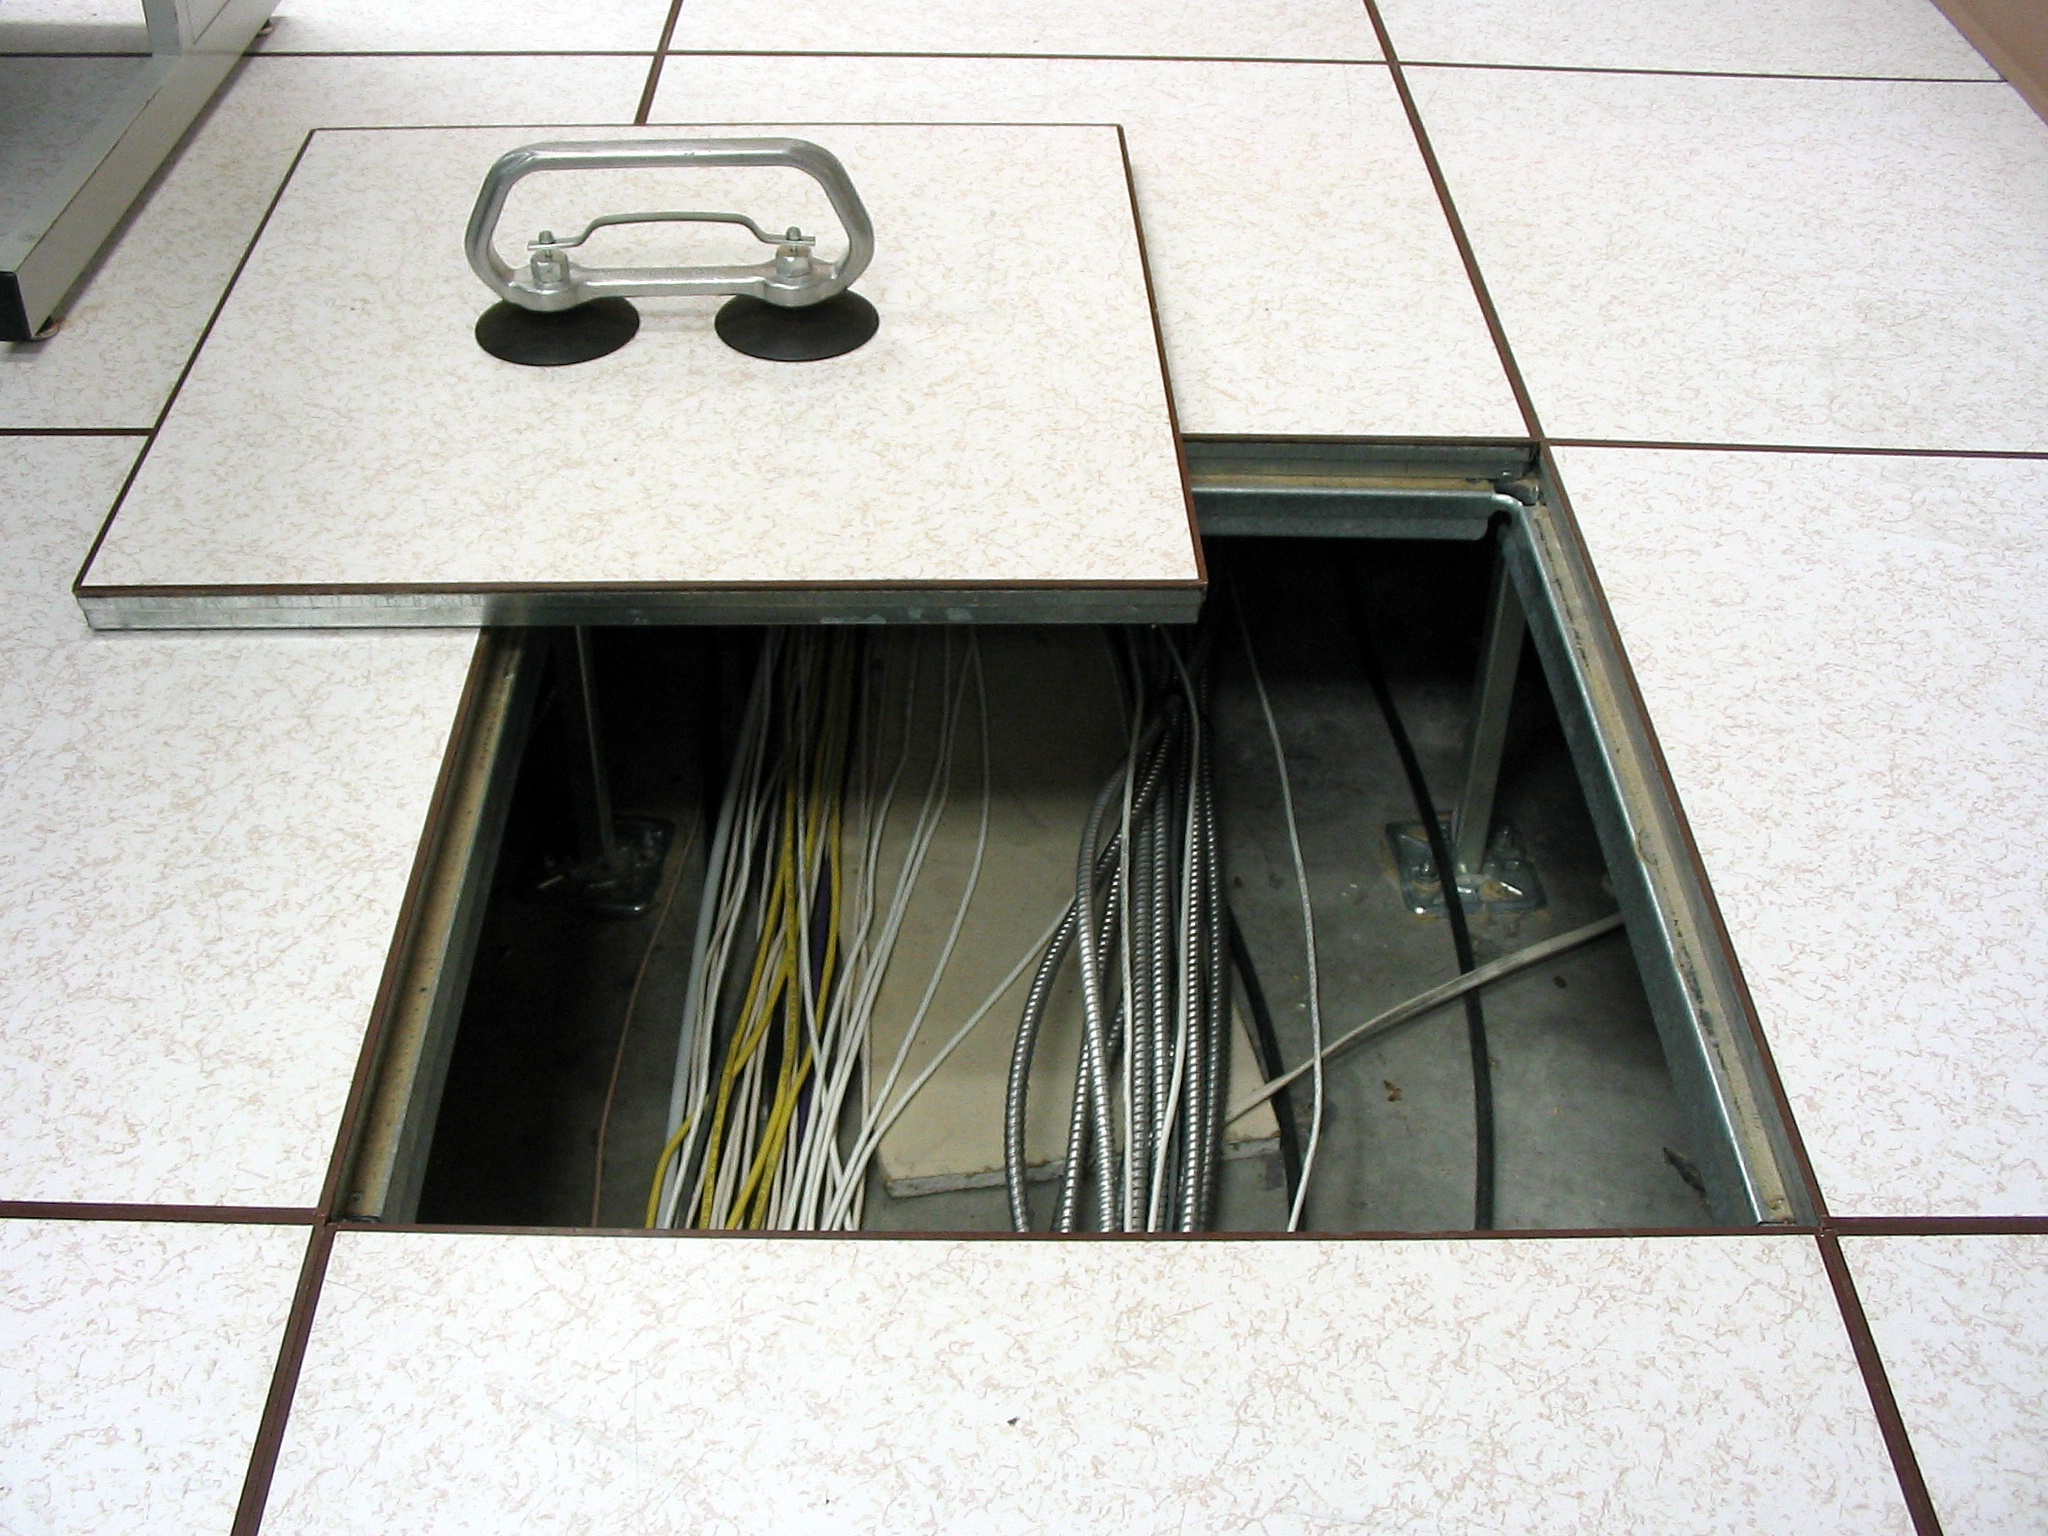
\includegraphics[keepaspectratio,alt={Pavimento flottante di un datacenter con mattonella sollevata}]{images/Tile-lifter-in-use-raised-floor-665fb3.jpg}}
\emph{Fonte: Wikimedia Commons (Jonathan Lamb, Public Domain) ---
Mattonella del pavimento flottante sollevata con ventosa; sotto sono
visibili cavi e condotte.}

Mantenere il pavimento flottante offre due vantaggi ingegneristici
fondamentali:

\begin{enumerate}
\def\labelenumi{\arabic{enumi}.}
\tightlist
\item
  \textbf{Accesso immediato} a tutta l'infrastruttura elettrica e
  idraulica nascosta sotto il pavimento, senza dover spostare i rack.
\item
  \textbf{Condotto di raffreddamento}: la cavità sotto il pavimento
  diventa un plenum isolato per spingere enormi quantità di aria fredda
  verso l'alto, attraverso mattonelle forate posizionate strategicamente
  davanti ai rack.
\end{enumerate}

Tenere i passaggi separati sotto il pavimento evita anche potenziali
cortocircuiti: il pericolo di innescare incendi è severo, specie in
presenza di batterie al litio --- notoriamente inestinguibili con le
procedure standard e severamente vietate nelle stive degli aerei proprio
per questo motivo.

\begin{center}\rule{0.5\linewidth}{0.5pt}\end{center}

\section{Strategie di Raffreddamento}\label{strategie-di-raffreddamento}

\subsection{Aria, Acqua e Olio}\label{aria-acqua-e-olio}

Per massimizzare l'efficienza termica, l'intero edificio del datacenter
viene isolato all'estremo dall'ambiente esterno. Non mancano eccezioni
creative: il complesso di Aruba, ad esempio, immette liberamente l'aria
gelida esterna in inverno ed espelle il flusso caldo verso fuori,
risparmiando energia.

Il principio fondamentale del raffreddamento a rack è la separazione
fisica tra \textbf{corridoio freddo} (\emph{cold aisle}) --- da cui i
server aspirano l'aria fresca --- e \textbf{corridoio caldo} (\emph{hot
aisle}) --- da cui espellono il calore. Questa separazione evita che
l'aria fredda e quella calda si mescolino prima di raggiungere i server,
massimizzando l'efficienza termica.

\pandocbounded{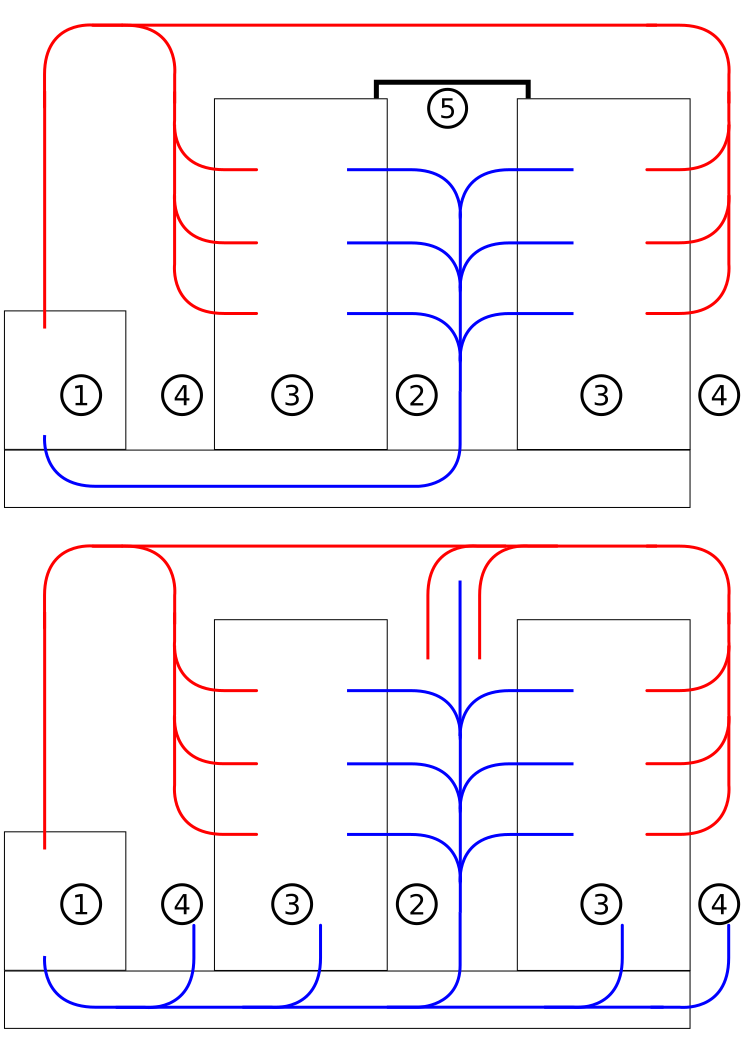
\includegraphics[keepaspectratio,alt={Diagramma hot aisle / cold aisle con contenimento del corridoio freddo}]{images/Cold-Aisle-Containment-e2b761.png}}
\emph{Fonte: Wikimedia Commons (CC BY-SA 3.0 DE) --- Schema di
contenimento del corridoio freddo: il flusso blu (aria fredda) entra dal
basso, attraversa i server e fuoriesce come flusso rosso (aria calda)
sul corridoio opposto.}

Dato che la logistica delle condotte idrauliche sta diventando
l'elemento centrale delle server farm moderne, si privilegia sempre di
più l'acqua per le sue eccezionali proprietà termiche. Ricalcando il
meccanismo biologico del sudore umano, i datacenter più grandi impiegano
attivamente la \textbf{dispersione tramite evaporazione}. Nonostante sia
una tecnica incredibilmente efficiente, il suo costo ambientale è
elevato: circa l'\textbf{80\% dell'acqua iniettata viene evaporata}.
Sebbene questa acqua ritorni nell'atmosfera come pioggia senza essere
distrutta, la dispersione massiccia locale crea sacche artificiali di
umidità che rischiano di alterare il microclima circostante.

\begin{calloutwarning}{Il problema idrico negli USA}

I massicci impieghi idrici agro-industriali combinati a quelli dei
datacenter hanno sostanzialmente prosciugato le risorse basate sul fiume
Colorado. Questo ha spinto alcune aziende a pianificare la migrazione
delle proprie sedi verso il Sud America --- Argentina in primis --- in
cerca di riserve idriche intoccate. L'acqua usata deve essere
desalinizzata e ripulita a fondo, il che aggiunge ulteriore complessità
logistica.

\end{calloutwarning}

Un'alternativa d'avanguardia è la \textbf{total immersion cooling}: i
server vengono immersi in vasche ricolme di olio minerale o vegetale. A
differenza dell'acqua, l'olio isola chimicamente i contatti e non
conduce elettricità, disperdendo il calore con grande efficacia ---
tecnica usata anche per overclock estremi nei PC da gaming.

\begin{calloutnote}{Limiti dell’immersion cooling}

\begin{itemize}
\tightlist
\item
  L'\textbf{olio vegetale} tende rapidamente a irrancidire, sprigionando
  odori acri.
\item
  L'\textbf{olio minerale} è molto costoso da approvvigionare in
  quantità industriali.
\item
  Ogni operazione di manutenzione su schede madri immerse diventa una
  procedura sporca e complessa.
\end{itemize}

Per queste ragioni, l'industria ha preferito affinare il raffreddamento
localizzato tramite tubazioni ad acqua pura anti-versamento,
accettandone la complessità tecnica.

\end{calloutnote}

\begin{center}\rule{0.5\linewidth}{0.5pt}\end{center}

\section{Infrastruttura Elettrica}\label{infrastruttura-elettrica-1}

\subsection{Scale Up vs Scale Out}\label{scale-up-vs-scale-out}

\begin{calloutdefinition}{Scale Up vs Scale Out}

\begin{itemize}
\tightlist
\item
  \textbf{Scale Up}: si aumenta la capacità di un singolo apparato (es.
  si aggiunge RAM a un server esistente).
\item
  \textbf{Scale Out}: si replica il numero di macchine separate per
  distribuire il carico (es. si aggiungono nuovi server al cluster).
\end{itemize}

\end{calloutdefinition}

Nel contesto dell'approvvigionamento elettrico, un intero edificio è
\textbf{costretto a operare in logica Scale Up}: all'aumentare del
consumo dell'infrastruttura, occorrono cavi di rame via via più
voluminosi e spessi. Scalare elettricamente è dolorosamente costoso,
soprattutto per il prezzo del rame. A titolo di esempio, il cablaggio
per supportare soli 80 kW di picco in un piccolo complesso accademico
--- trascinando il fascio dalla cabina esterna ai server --- è arrivato
a costare circa \textbf{25.000 €}. Per minimizzare la resistenza
elettrica intrinseca con correnti molto elevate, i tecnici sostituiscono
i fasci di cavi intrecciati con \textbf{sbarre di rame pieno}
(\emph{busbars}), singole e dritte.

\subsection{Fondamenti Elettrici: Potenza, Corrente Alternata e
Distribuzione}\label{fondamenti-elettrici-potenza-corrente-alternata-e-distribuzione}

Un datacenter richiede una concentrazione energetica enorme, che può
essere fornita da rinnovabili, combustibili fossili o nucleare. Nelle
logiche macro-aziendali americane in espansione, si intravede l'uso di
reattori di ultimissima generazione --- tecnologicamente più puri e
sicuri, con materiali radioattivi come il torio --- che generano circa
un decimo delle scorie rispetto all'uranio tradizionale.

Per gestire questo flusso, l'ingegnere deve dominare il concetto di
\textbf{potenza effettiva}, che non si ricava semplicemente dai Volt, ma
dal prodotto:

\[
P_{\text{apparente}} = V \times I \quad [\text{VA}]
\]

\[
P_{\text{reale}} = V \times I \times \cos\phi \quad [\text{W}]
\]

dove \(\cos\phi\) (\textbf{Cosfi}, o \emph{fattore di potenza}) è il
coseno dell'angolo di sfasamento tra tensione e corrente. I moderni
trasformatori \emph{switching} --- presenti sia nei server farm sia nel
piccolo alimentatore del laptop --- hanno un Cosfi variabile: scende a
circa \textbf{0.56} quando i componenti sono inattivi (\emph{idle}), ma
sale fino a \textbf{0.96} sotto carico computazionale intenso.

\begin{callouttip}{Perché il Cosfi è cruciale negli acquisti}

Durante le gare di acquisto per apparecchiature industriali, esigere
trasformatori con un elevato \emph{power factor} è una scelta
economicamente discriminante: apparecchi con basso Cosfi disperdono una
quota significativa dell'energia prelevata dalla rete, aumentando i
costi operativi nel lungo periodo.

\end{callouttip}

Nonostante l'elettronica digitale lavori esclusivamente in
\textbf{Corrente Continua} (\emph{DC --- Direct Current}), tutti i
datacenter globali ricevono energia in \textbf{Corrente Alternata
Trifase} (\emph{AC --- Alternating Current}), standardizzata a
\textbf{380 V} in Europa. Le ragioni sono storiche e fisiche: far
transitare enormi flussi di corrente continua scalda i conduttori in
modo molto più pericoloso, e le scosse in DC sono fisiologicamente più
letali di quelle in AC a parità di energia. Sarà ogni singolo server,
nell'ultima maglia della rete, a convertire la corrente alternata in
continua attraverso il proprio alimentatore interno.

\begin{calloutdefinition}{UPS (Uninterruptible Power Supply)}

Componente al vertice della piramide di distribuzione elettrica del
datacenter. Non si tratta dei piccoli dispositivi domestici
anti-blackout, ma di \textbf{interi armadi e batterie industriali}
destinati a stabilizzare la linea e garantire continuità in caso di
interruzione della rete esterna. Gli interruttori di sezionamento ---
talmente potenti da non poter essere azionati manualmente a mani nude
--- vengono commutati da \textbf{molle metalliche precompresse}, che il
meccanismo rilascia automaticamente per garantire la massima velocità di
intervento e proteggere il personale.

\end{calloutdefinition}

\begin{calloutdefinition}{PDU (Power Distribution Unit)}

Centraline di gestione che suddividono progressivamente il carico
elettrico lungo la gerarchia di distribuzione. La rete elettrica segue
un'architettura ad albero: dalla cabina esterna si scende attraverso PDU
di piano, fino ai \textbf{Rack PDU} dove ogni server inserisce il
proprio cavo di alimentazione.

\end{calloutdefinition}

L'architettura di distribuzione elettrica segue quindi questo percorso
gerarchico:

\textbf{Rete Trifase Esterna → UPS → PDU di edificio → PDU di piano →
Rack PDU → Server}

\begin{calloutnote}{Sintesi — Infrastruttura Elettrica}

La progettazione elettrica di un datacenter è vincolata da hard
threshold fisici non aggirabili: cavi più grossi, costosi e difficili da
gestire. La corrente arriva dall'esterno in AC trifase a 380 V, viene
stabilizzata dall'UPS e distribuita gerarchicamente tramite PDU fino ai
server, che la convertono in DC internamente. Il fattore di potenza è
una metrica economica critica da valutare in fase di acquisto delle
apparecchiature.

\end{calloutnote}

\begin{center}\rule{0.5\linewidth}{0.5pt}\end{center}

\section{Glossario}\label{glossario-1}

\begin{calloutdefinition}{Scale Up / Scale Out}

Tecniche per rispondere al fabbisogno crescente di risorse.
\textbf{Scale Up} aumenta la capacità di un singolo nodo (più RAM, CPU
più potente); \textbf{Scale Out} distribuisce il carico su un numero
maggiore di nodi separati. In ambito elettrico, i datacenter sono
forzati a operare in Scale Up, con tutti i costi che ne derivano.

\end{calloutdefinition}

\begin{calloutdefinition}{CIA Triad (Disponibilità, Integrità, Riservatezza)}

Il trittico fondamentale su cui si basa la progettazione protettiva dei
servizi digitali. Garantire \textbf{Disponibilità} significa che il
servizio è sempre raggiungibile; \textbf{Integrità} significa che i dati
sono corretti e non manomessi; \textbf{Riservatezza} significa che solo
i soggetti autorizzati possono accedervi. Il GDPR sanziona la violazione
di ciascuno dei tre pilastri.

\end{calloutdefinition}

\begin{calloutdefinition}{Fattore di Potenza (Cosfi, \\cos\\phi)}

Rapporto tra la potenza reale (W) e la potenza apparente (VA):
\(\cos\phi = P / S\). Quantifica quanto efficacemente l'energia
prelevata dalla rete viene effettivamente convertita in lavoro utile. Un
Cosfi basso indica dispersione energetica. Nei trasformatori switching
dei server, varia tra \textasciitilde0.56 (idle) e \textasciitilde0.96
(sotto carico).

\end{calloutdefinition}

\begin{calloutdefinition}{Floating Floor (Pavimento Flottante)}

Struttura rialzata del datacenter su piedistalli metallici, con
mattonelle rimovibili che reggono fino a 1--1,5 t/m². Serve un duplice
scopo: accesso facilitato all'infrastruttura nascosta sotto il
pavimento, e creazione di un plenum per la distribuzione dell'aria
fredda di raffreddamento verso i rack.

\end{calloutdefinition}

\begin{calloutdefinition}{UPS (Uninterruptible Power Supply)}

Primo stadio di ingresso della rete elettrica nel datacenter. Sistema
industriale di grosse dimensioni --- non il piccolo dispositivo
domestico --- composto da batterie e meccanismi di commutazione
automatica, progettato per garantire continuità di alimentazione e
proteggere l'intera infrastruttura da fluttuazioni e blackout della rete
esterna.

\end{calloutdefinition}

\newpage

\chapter{Gestione dell'Energia e del Raffreddamento nei Data
Center}\label{gestione-dellenergia-e-del-raffreddamento-nei-data-center}

L'infrastruttura di un Data Center moderno è un ecosistema estremamente
complesso, paragonabile a un'orchestra in cui ogni elemento ---
alimentazione, reti, raffreddamento e rack --- deve funzionare in
perfetta armonia con gli altri. In questo capitolo esploreremo le
dinamiche fisiche, economiche e gestionali che governano alimentazione e
raffreddamento: dal mercato dei fornitori e dalle criticità della
manutenzione, al rischio del surriscaldamento, ai parametri di
efficienza energetica come il \textbf{PUE} (\emph{Power Usage
Effectiveness}), fino all'evoluzione delle architetture di
condizionamento ad aria con i sistemi \textbf{CRAC}.

\begin{center}\rule{0.5\linewidth}{0.5pt}\end{center}

\section{Il Mercato dei Vendor e la Strategia di
Acquisizione}\label{il-mercato-dei-vendor-e-la-strategia-di-acquisizione}

Acquistare le singole parti di un Data Center per assemblarle
autonomamente è un errore strategico considerevole. Poiché ogni
componente influenza direttamente gli altri, è fondamentale affidarsi a
ecosistemi integrati forniti da vendor specializzati. Al giorno d'oggi
ogni parte del Data Center è considerabile ``attiva'': anche elementi
passivi come rack e schede di controllo sono dotati di display e
interfacce accessibili via protocollo HTTP.

Esistono pochi fornitori al mondo capaci di gestire le competenze
necessarie per installazioni ad alta potenza. \textbf{Schneider
Electric} domina le installazioni elettriche e ha acquisito \textbf{APC}
(storica azienda specializzata in rack e gruppi di continuità). Un altro
colosso è \textbf{Vertiv} (ex Emerson), nata come produttrice di
\emph{chiller} (refrigeratori industriali). In Italia il mercato è
presidiato da \textbf{Riello} per sistemi elettrici e UPS, e
\textbf{Climaveneta} per i chiller.

\begin{center}\rule{0.5\linewidth}{0.5pt}\end{center}

\section{La Manutenzione e il Ciclo di
Vita}\label{la-manutenzione-e-il-ciclo-di-vita}

Quando si acquista un Data Center, in realtà non si compra solo
hardware: si ``sposa'' il produttore attraverso un contratto di
manutenzione. Il modello di business è analogo a quello delle automobili
di fascia alta --- BMW o Mercedes --- dove l'accesso alle centraline e
la riparazione richiedono strumenti proprietari che solo il produttore
può fornire.

\begin{calloutwarning}{Costi dell’infrastruttura}

I costi sono imponenti: la ristrutturazione di un DC di piccole
dimensioni parte da circa \textbf{250.000--300.000 €}, mentre impianti
più grandi oscillano tra \textbf{2 e 5 milioni di €}. Acquistare un
pezzo di ricambio da tenere in magazzino --- per esempio un chiller da
\textbf{100.000 €} --- è economicamente insostenibile e logisticamente
impraticabile per via degli ingombri fisici.

\end{calloutwarning}

I contratti di manutenzione garantiscono interventi ``Next Business
Day'' o entro \textbf{4 ore}, con monitoraggio remoto 24/7. Il costo
annuo di questi contratti oscilla tra il \textbf{10\% e il 30\%}
dell'investimento originale. Se si decide di non rinnovare, dopo alcuni
anni i vendor non garantiscono più la disponibilità dei ricambi ---
specialmente per macchine con oltre \textbf{12 anni} di vita ---
costringendo di fatto l'operatore a un costoso aggiornamento totale. Il
ciclo di vita tipico di un intero Data Center si aggira intorno ai
\textbf{10 anni}.

\begin{center}\rule{0.5\linewidth}{0.5pt}\end{center}

\section{Surriscaldamento: Una Minaccia Critica per il
Silicio}\label{surriscaldamento-una-minaccia-critica-per-il-silicio}

Dal punto di vista concettuale, un Data Center richiede le stesse
risorse di un'abitazione domestica: rete, corrente, raffreddamento. La
differenza è nella scala: mentre un contatore domestico eroga
\textbf{3--5 kW}, un Data Center necessita facilmente di \textbf{1
Megawatt} per alimentare migliaia di server.

Questo fabbisogno energetico massiccio si traduce in un enorme rilascio
di calore. Se il sistema di raffreddamento si guasta, la situazione
degenera rapidamente: le ventole dei server, dotate di sensori termici,
percepiscono l'aumento di temperatura e accelerano per compensare. Ma
spostando aria già calda, il loro stesso attrito immette ulteriore
energia termica nella stanza. Si innesca un \textbf{effetto
esponenziale}: in assenza di aria fredda, la temperatura della sala può
raggiungere \textbf{60--70°C} in tempi brevissimi, a tal punto che
l'unica soluzione di emergenza è l'apertura fisica delle porte
dell'edificio.

\begin{calloutwarning}{Surriscaldamento vs. blackout}

Il surriscaldamento è storicamente più pericoloso di una semplice
interruzione di corrente. Un blackout tradizionale danneggiava i dischi
rigidi meccanici --- la testina rischiava di graffiare il piatto al
momento dello stop improvviso --- ma con la diffusione degli
\textbf{SSD} questa mortalità si è drasticamente ridotta. Il calore
estremo, invece, può sciogliere i componenti plastici e danneggiare
irreparabilmente il \textbf{silicio} delle componenti elettroniche,
rendendole inutilizzabili.

\end{calloutwarning}

\begin{callouttip}{La termodinamica del rack a 40°C}

Alcuni vendor certificano che i server, con vita utile media di
\textbf{5 anni}, possano operare per \textbf{40 giorni all'anno a 40°C}.
Sembra un limite elevato, ma bisogna considerare il \textbf{Delta T} del
rack: la differenza di temperatura tra l'aria fredda in ingresso
(\emph{inlet}) e l'aria espulsa sul retro è tipicamente di circa
\textbf{15°C}. Se l'aria in ingresso è a 40°C, sul retro del rack si
raggiungono facilmente 55--60°C. I dischi meccanici per \emph{cold
storage} (archiviazione economica) possono arrivare a temperature
superficiali operative di \textbf{100°C} --- letteralmente abbastanza
calde da cuocerci sopra.

\end{callouttip}

\begin{callouttip}{Il guasto dei chiller pisani}

Durante una settimana di luglio con temperature esterne superiori ai
\textbf{38°C}, i vecchi chiller del Data Center pisano --- progettati in
anni in cui quei picchi non si registravano --- sono andati in blocco
termico perché le loro dimensioni non consentivano di dissipare un tale
carico. In sole \textbf{due ore} la sala macchine ha raggiunto i
\textbf{50°C}, costringendo a spegnere tutto e a versare letteralmente
acqua fredda sulle scocche dei chiller per poterli riavviare. Questo
episodio dimostra quanto i servizi Internet siano vulnerabili alle
condizioni fisiche dell'ambiente.

\end{callouttip}

\begin{center}\rule{0.5\linewidth}{0.5pt}\end{center}

\section{Anomalie Elettriche e i
``Bug''}\label{anomalie-elettriche-e-i-bug}

Non solo il calore, ma anche le interruzioni elettriche causano gravi
disservizi. I \textbf{UPS} (\emph{Uninterruptible Power Supply}, gruppi
di continuità) intervengono durante le micro-interruzioni di rete per
dare il tempo ai generatori diesel di avviarsi. In un caso specifico,
continue micro-interruzioni da \textbf{10--15 secondi} non furono
tollerate dall'elettronica di controllo dei chiller --- non messi sotto
UPS per motivi di costo. I chiller, interpretando quel disturbo come un
pericolo, si spensero autonomamente, causando la caduta di tre impianti
di refrigerazione. La soluzione fu l'acquisto di un UPS dedicato
esclusivamente ai chiller per stabilizzarne l'alimentazione.

\begin{callouttip}{L’origine del termine “bug”}

Un serpente in cerca di calore durante l'inverno si infilò in una cabina
di distribuzione ad alta tensione, attaccandosi alle bobine e causando
un cortocircuito fatale che spense l'intero Data Center --- lasciando a
terra solo il proprio corpo carbonizzato. Il termine informatico
\textbf{``bug''} deriva proprio da questo tipo di incidenti: veri
insetti e roditori che causavano blackout masticando cavi o
cortocircuitando componenti.

\end{callouttip}

\begin{center}\rule{0.5\linewidth}{0.5pt}\end{center}

\section{L'Efficienza Energetica e il
PUE}\label{lefficienza-energetica-e-il-pue}

Sprecare energia non comporta solo perdite economiche dirette, ma impone
costi indiretti: componenti elettriche e cavi più spessi e costosi per
reggere i picchi. In uno scenario in cui i costi energetici sono passati
da \textbf{300.000 € a 1.000.000 € all'anno} --- complice il conflitto
in Ucraina --- misurare l'efficienza è diventato cruciale.

\begin{calloutdefinition}{PUE — Power Usage Effectiveness}

Il \textbf{PUE} è il parametro adimensionale standard per misurare
l'efficienza energetica di un Data Center. Si calcola come:

\[
\text{PUE} = \frac{\text{Total Facility Power}}{\text{IT Equipment Power}}
\]

Il \emph{Total Facility Power} è la somma del consumo IT,
dell'illuminazione e --- soprattutto --- del dispendio per il
raffreddamento. Poiché l'assorbimento IT compare sia al numeratore che
al denominatore, il valore ideale teorico in assenza di overhead è
\textbf{1}. Il PUE è sempre maggiore di 1: più alto è il valore,
peggiore è l'efficienza. Alcuni utilizzano l'inverso della formula per
ottenere un indice compreso tra 0 e 1, ma il concetto non muta.

\end{calloutdefinition}

{\def\LTcaptype{none} % do not increment counter
\begin{longtable}[]{@{}
  >{\raggedright\arraybackslash}p{(\linewidth - 2\tabcolsep) * \real{0.5000}}
  >{\raggedright\arraybackslash}p{(\linewidth - 2\tabcolsep) * \real{0.5000}}@{}}
\toprule\noalign{}
\begin{minipage}[b]{\linewidth}\raggedright
Valore PUE
\end{minipage} & \begin{minipage}[b]{\linewidth}\raggedright
Interpretazione
\end{minipage} \\
\midrule\noalign{}
\endhead
\bottomrule\noalign{}
\endlastfoot
≤ 1.2 & Eccellente --- standard moderno \\
\textless{} 1.3 & Raccomandato dall'UE per DC Hyperscale \\
1.15 & PUE annuo del Green DC Università di Pisa a pieno carico \\
1.8 -- 2.0 & Valore medio italiano --- molto negativo \\
\textgreater{} 2.0 & Per ogni kW di IT si spende più di 1 kW solo per
raffreddarlo \\
\end{longtable}
}

\subsection{Le Insidie del PUE}\label{le-insidie-del-pue}

Sebbene essenziale, il PUE può nascondere informazioni fuorvianti. La
prima domanda da porsi davanti a qualsiasi valore dichiarato è:
\emph{``Su quale arco temporale e a quali condizioni è stato
misurato?''}

\begin{calloutwarning}{Trappole nel confronto tra PUE}

\textbf{Impatto stagionale.} Refrigerare d'inverno costa molto meno che
d'estate. Esibire un PUE istantaneo misurato a gennaio (es. 1.05) è
``barare''. È necessario calcolare un \textbf{PUE annuo} (\emph{Yearly
PUE}), mediando la curva stagionale lungo l'intero anno. In Europa il
picco dei consumi è in estate; in Australia --- con le stagioni traslate
di sei mesi --- il picco cade tra dicembre e gennaio.

\textbf{Saturazione del Data Center.} Un DC quasi vuoto (es. con un solo
server) può mostrare un PUE pessimo perché il compressore dei chiller
gira ``a vuoto'' rispetto al carico IT. Al contrario, lo stesso DC pieno
lavorerà all'efficienza progettata.

\textbf{Dimensioni dell'impianto.} Per un piccolo rack di 5 server con
un budget di \textbf{1.000.000 € annui}, potrebbe essere economicamente
più vantaggioso installare un normale condizionatore domestico ---
accettando un PUE di 2.0 --- piuttosto che affrontare l'investimento
multimilionario di un impianto industriale ottimizzato.

\end{calloutwarning}

\begin{center}\rule{0.5\linewidth}{0.5pt}\end{center}

\section{Data Center Orbitali: il PUE
Perfetto}\label{data-center-orbitali-il-pue-perfetto}

L'ossessione per il PUE ha spinto aziende a progettare \textbf{Data
Center Orbitali nello spazio}. In assenza di atmosfera, lo smaltimento
del calore e l'assorbimento dell'energia solare sono enormemente
facilitati, permettendo di avvicinarsi a un PUE teorico di \textbf{1}
(valori realistici stimati: 1.01--1.07). Questi sistemi avrebbero un
ciclo di vita di \textbf{10--15 anni}, al termine del quale i moduli
verrebbero de-orbitati per bruciare nell'atmosfera o --- idealmente ---
recuperati e sostituiti.

\begin{calloutnote}{Latenza nelle comunicazioni orbitali}

Per comunicazioni \emph{point-to-point}, la latenza non sarebbe un
problema insormontabile: la luce percorre distanze nell'aria pressoché
istantaneamente, mentre viaggia a circa \textbf{0.6c} nei cavi in rame a
terra. La vera sfida attuale rimane la quantità di detriti in orbita
(\emph{orbital debris}), che rende pericolosa qualsiasi installazione
stabile.

\end{calloutnote}

\begin{center}\rule{0.5\linewidth}{0.5pt}\end{center}

\section{L'Architettura ad Aria: Sistemi
CRAC}\label{larchitettura-ad-aria-sistemi-crac}

Poiché l'acqua è un conduttore termico nettamente superiore all'aria ---
che funge anzi da ottimo isolante termico --- il raffreddamento ad aria
è economico ma decisamente non ottimale. Negli anni '90 si mantenevano
temperature di sala macchine di circa \textbf{17°C}; oggi lo standard
operativo si attesta a \textbf{26--27°C}. Nel 2000, nel data center
Tiscali in Sardegna, un rack consumava appena \textbf{3 kW} e lo si
raffreddava tenendo le finestre aperte. Con l'innalzamento delle potenze
(\emph{High Density Computing}), si sono rese necessarie architetture
più sofisticate.

\begin{calloutdefinition}{CRAC — Computer Room Air Conditioning}

Il \textbf{CRAC} è la prima architettura industriale di raffreddamento
ad aria, ancora in uso in strutture classiche --- come alcuni building
Aruba, con carichi web server prevedibili di circa 300 W per server.
Prevede macchinari verticali disposti nella stanza, un \textbf{pavimento
sopraelevato} (\emph{raised floor} o \emph{floating floor}) e piastrelle
forate (\emph{perforated tiles}) posizionate con cura di fronte ai rack.

\end{calloutdefinition}

Il principio fisico alla base è la \textbf{convezione}: l'aria calda
tende naturalmente a salire. Il ciclo di funzionamento è il seguente: il
macchinario CRAC aspira l'aria calda dalla parte alta della stanza,
genera aria fredda e la immette a pressione al di sotto del pavimento
flottante. L'aria fredda viaggia nel \emph{plenum} sottostante e risale
solo attraverso le piastrelle perforate poste di fronte ai rack.

\pandocbounded{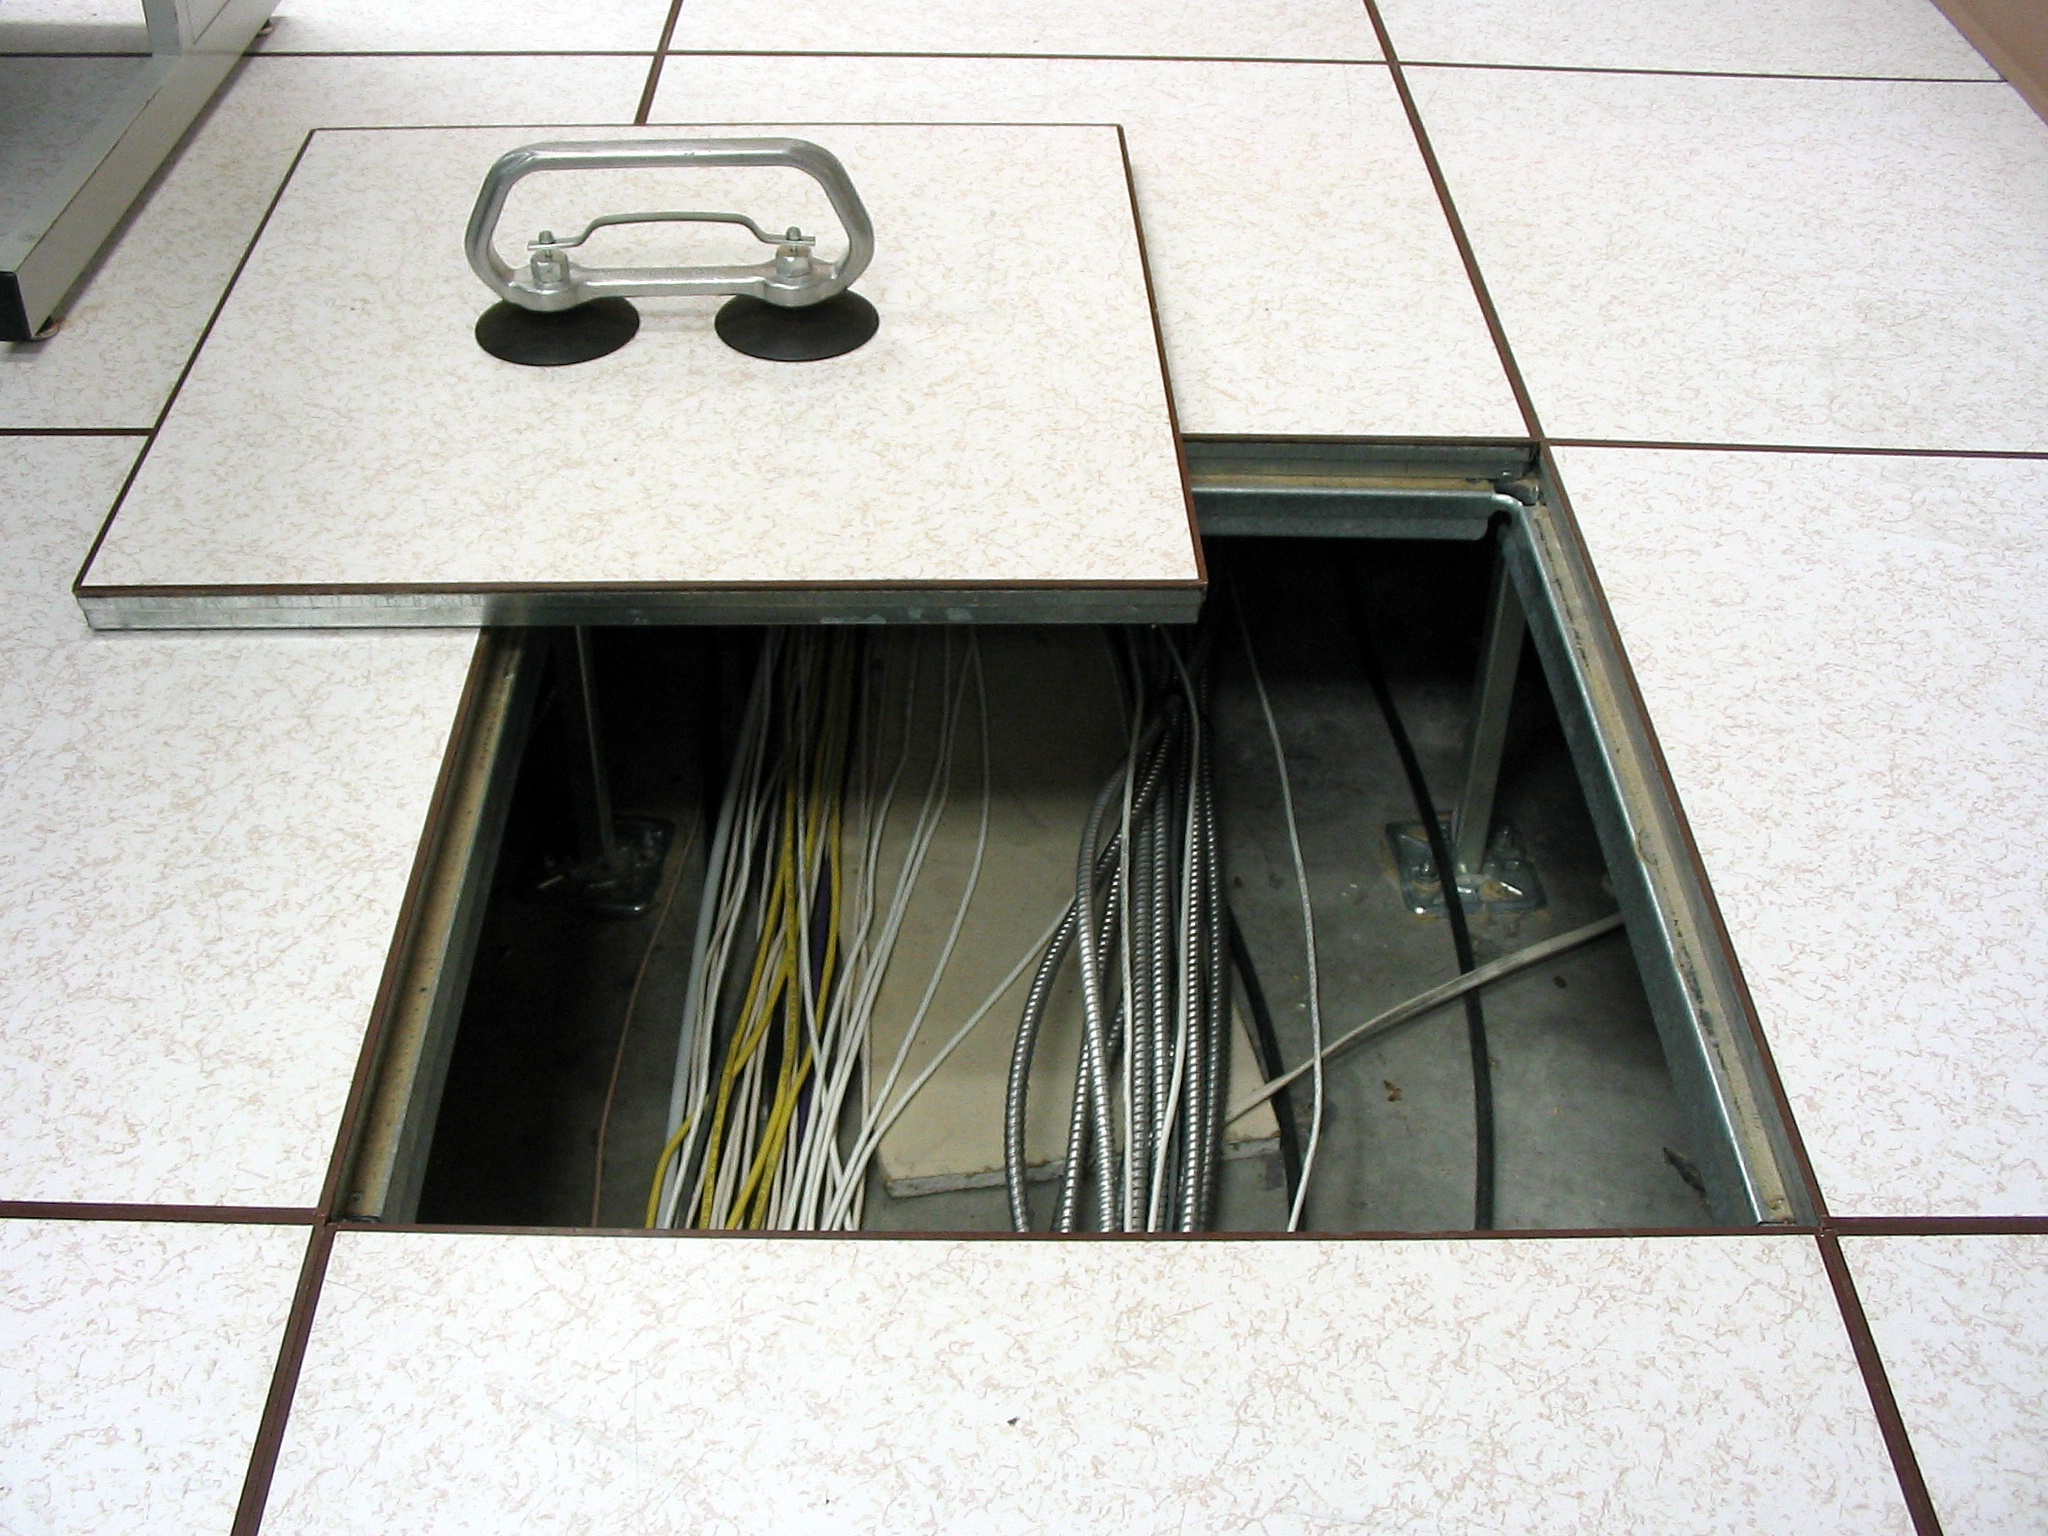
\includegraphics[keepaspectratio,alt={Sollevamento di una piastrella dal pavimento sopraelevato (raised floor) di un data center}]{images/Tile-lifter-in-use-raised-floor-878fd6.jpg}}
\emph{Fig. --- Il pavimento sopraelevato (}raised floor\emph{) è la
caratteristica strutturale che rende possibile il sistema CRAC: il
}plenum* sottostante distribuisce l'aria fredda verso le piastrelle
perforate posizionate davanti ai rack.* Viene poi aspirata dalle ventole
frontali dei server, li raffredda, ed esce come aria calda sul retro,
risalendo verso il soffitto per ricominciare il ciclo.

\begin{callouttip}{La regola d’oro del CRAC}

\textbf{Non mescolare mai aria calda con aria fredda.} Mescolare i due
flussi annullerebbe il lavoro termodinamico speso per generare il
raffreddamento, abbassando drasticamente l'efficienza. In alcuni DC
specializzati come quelli Aruba, i rack sono dotati di una porta
frontale in vetro antiesplosione con griglie di aerazione posizionate
\emph{all'interno} --- tra il cristallo e i server --- per canalizzare
chirurgicamente il flusso freddo direttamente nell'IT senza dispersioni.

\end{callouttip}

\begin{calloutwarning}{Il limite dell’architettura CRAC}

Con le odierne densità di potenza --- fino a decine di kW per rack ---
lo spazio fisico si satura. Se il soffitto non è abbastanza alto e il
\emph{plenum} sotto il pavimento non è sufficientemente profondo, il
volume d'aria calda diventa così imponente che la convezione viene
vinta: l'aria calda scende di nuovo sui server, mandando il sistema in
blocco termico. L'architettura CRAC incontra quindi un limite
strutturale nelle installazioni \emph{high-density} moderne.

\end{calloutwarning}

\begin{center}\rule{0.5\linewidth}{0.5pt}\end{center}

\begin{calloutnote}{Sintesi}

La gestione dell'energia e del raffreddamento in un Data Center
intreccia fisica termodinamica, economia e ingegneria dei sistemi. Il
\textbf{PUE} è lo strumento standard per misurare l'efficienza, ma va
sempre interpretato su base annua e in relazione al carico effettivo ---
un valore istantaneo è quasi sempre fuorviante. Le architetture di
raffreddamento, dai sistemi \textbf{CRAC} tradizionali a soluzioni più
moderne, devono affrontare densità di potenza crescenti mantenendo la
separazione netta tra flussi di aria calda e fredda. Il \emph{vendor
lock-in} e i contratti di manutenzione rappresentano il vero costo
nascosto di un'infrastruttura che, per sua natura, non può mai fermarsi.

\end{calloutnote}

\newpage

\chapter{Densità, Calore e Raffreddamento Avanzato nei Data Center
Moderni}\label{densituxe0-calore-e-raffreddamento-avanzato-nei-data-center-moderni}

L'industria dei data center sta attraversando una trasformazione
radicale guidata da un fattore fisico incontrovertibile: la densità di
potenza per rack è aumentata di un ordine di grandezza nell'arco di un
decennio. Comprendere questa trasformazione richiede partire dai
fondamenti fisici del silicio per poi risalire alle scelte
architetturali e infrastrutturali che ne conseguono.

\section{I Limiti Fisici del Silicio}\label{i-limiti-fisici-del-silicio}

\subsection{Il Muro della Frequenza}\label{il-muro-della-frequenza}

L'industria dei semiconduttori si trova a confrontarsi con vincoli
fisici che non sono aggirabili con la sola ingegneria. I processi
litografici si sono spinti fino ai 2 nanometri, una scala alla quale gli
effetti quantistici e le interferenze termiche diventano critici. Sul
piano delle frequenze di clock, le CPU hanno raggiunto un plateau
pratico attorno ai 2--4 GHz: spingersi oltre genera un numero
insostenibile di errori logici e un'emissione elettromagnetica che
inizia a sfiorare lo spettro dei raggi X.

\begin{calloutwarning}{Il plateau delle frequenze}

Aumentare la frequenza di clock oltre i 4 GHz non è semplicemente
difficile --- è fisicamente pericoloso per l'integrità dei transistor e
produce interferenze elettromagnetiche inaccettabili. Questo spiega
perché l'industria ha virato sul parallelismo multi-core invece di
puntare sulla velocità del singolo core.

\end{calloutwarning}

La risposta dell'industria è stata il calcolo parallelo: aumentare il
numero di core piuttosto che la velocità di ogni singolo core. Tuttavia
questa soluzione non risolve tutti i problemi. Esistono classi di
carichi di lavoro --- come le simulazioni Monte Carlo al CERN --- che
non sono parallelizzabili per natura e richiedono ancora poche CPU ad
altissima frequenza. Questo crea un mercato di nicchia ma cruciale per
processori single-core ad alte prestazioni.

\begin{center}\rule{0.5\linewidth}{0.5pt}\end{center}

\section{L'Impatto dell'Intelligenza Artificiale sui Data
Center}\label{limpatto-dellintelligenza-artificiale-sui-data-center}

\subsection{TDP e Densità Estrema}\label{tdp-e-densituxe0-estrema}

L'esplosione delle reti neurali profonde e dei \textbf{Large Language
Model (LLM)} ha ridefinito completamente i parametri di progettazione
dei data center. Il \textbf{TDP} (\emph{Thermal Design Power} --- potere
termico di progetto) indica il calore massimo che un sistema di
raffreddamento deve essere in grado di dissipare per mantenere il
processore entro i limiti operativi. Questo parametro è cresciuto
esponenzialmente: le moderne CPU top di gamma raggiungono i 500 Watt,
mentre le GPU di nuova generazione (come le architetture NVIDIA
Blackwell) superano 1 Kilowatt per singolo processore.

La densità raggiunte dai nodi moderni è straordinaria: un singolo server
AI equipaggiato con CPU, svariate GPU e storage ad alta velocità può
contenere fino a 18 trilioni di transistor in un volume di pochi rack
unit.

\begin{calloutnote}{Co-evoluzione dell’architettura di sistema}

Per alimentare questi processori senza colli di bottiglia, l'intera
architettura si è evoluta in modo coordinato. Lo standard PCIe ha
aggiornato rapidamente le proprie specifiche, e l'introduzione di
memorie non volatili (NVDIMM) e SSD ultra-veloci ha praticamente
dissolto i confini tra i vecchi livelli della gerarchia di memoria
tradizionale, rendendo il concetto stesso di ``gerarchia'' meno rigido
di quanto fosse un decennio fa.

\end{calloutnote}

\begin{center}\rule{0.5\linewidth}{0.5pt}\end{center}

\section{La Transizione al Raffreddamento a
Liquido}\label{la-transizione-al-raffreddamento-a-liquido}

A causa della densità di transistor raggiunta dai processori moderni,
l'aria --- che è un mediocre conduttore di calore e si comporta di fatto
come un isolante termico --- non è più fisicamente in grado di smaltire
il calore all'interno dei rack. L'industria ha compiuto una transizione
strutturale verso il \textbf{liquid cooling} (raffreddamento a liquido),
che si articola in diverse tecnologie con caratteristiche e compromessi
ben distinti.

\subsection{Direct-to-Chip}\label{direct-to-chip}

Il sistema \textbf{Direct-to-Chip} porta il fluido refrigerante a
diretto contatto con i componenti che generano calore, eliminando quasi
totalmente le ventole. Soluzioni come \emph{Lenovo Neptune} utilizzano
reti di tubi e piastre in puro rame posizionate direttamente su CPU, GPU
e banchi di memoria RAM. Il risultato è un'efficienza termica nettamente
superiore rispetto ai sistemi ad aria, con una riduzione significativa
del rumore e del consumo energetico delle ventole.

\subsection{Waterless Cooling}\label{waterless-cooling}

Per evitare i catastrofici danni hardware dovuti a eventuali perdite
d'acqua --- un'eventualità reale in ambienti che operano 24/7 --- sono
stati sviluppati sistemi basati su \textbf{fluidi dielettrici} come il
glicole. Questi liquidi, a differenza dell'acqua, non conducono
elettricità: un eventuale sversamento non causa cortocircuiti né
incendi. Le loro proprietà fisiche consentono inoltre l'uso di tubazioni
molto più sottili rispetto ai circuiti idraulici tradizionali,
semplificando il routing interno al rack.

\subsection{Immersion Cooling}\label{immersion-cooling}

Il metodo più radicale prevede l'immersione fisica dei server in vasche
di \textbf{olio minerale} dielettrico. Il centro di calcolo TACC in
Texas è uno degli esempi più noti di questa tecnologia. L'efficienza
termica è estrema: l'olio circonda uniformemente ogni componente,
eliminando ogni punto caldo localizzato. Il prezzo da pagare è la
complessità operativa: il costo dell'olio è elevato, la manutenzione
richiede procedure dedicate e ogni componente estratto risulta
inevitabilmente rivestito di olio.

\begin{callouttip}{Scegliere il metodo di raffreddamento}

La scelta tra Direct-to-Chip, Waterless e Immersion Cooling non è solo
tecnica ma anche economica e operativa. Il Direct-to-Chip è il
compromesso più bilanciato per la maggior parte dei data center HPC;
l'Immersion Cooling si giustifica solo per densità estreme e carichi di
lavoro uniformi e prevedibili.

\end{callouttip}

\subsection{Manutenzione Idraulica}\label{manutenzione-idraulica}

L'introduzione dei circuiti d'acqua trasforma il profilo di competenze
richiesto ai team di gestione. L'acqua minerale comune tende a
depositare incrostazioni di calcio che rischiano di ostruire tubi con
diametri nell'ordine di pochi centimetri. I circuiti devono essere
sottoposti a severi test di pressurizzazione a gas prima
dell'attivazione per escludere perdite, e richiedono l'intervento
periodico di idraulici specializzati --- una figura professionale del
tutto estranea al tradizionale mondo IT.

\begin{center}\rule{0.5\linewidth}{0.5pt}\end{center}

\section{La Sfida Energetica e le AI
Factories}\label{la-sfida-energetica-e-le-ai-factories}

\subsection{Consumi su Scala
Industriale}\label{consumi-su-scala-industriale}

Le infrastrutture dedicate all'addestramento di modelli AI non sono più
classificabili come semplici data center: sono vere e proprie \textbf{AI
Factories}, impianti industriali che richiedono potenze nell'ordine di
1--2 Gigawatt. Per dare una misura concreta, 1 Gigawatt corrisponde al
consumo elettrico di una città di circa un milione di abitanti.

\begin{callouttip}{Consumo idrico dell’addestramento AI}

Per dissipare il calore prodotto durante l'addestramento di un singolo
grande modello, le torri di raffreddamento evaporativo consumano
quantità d'acqua paragonabili a intere piscine olimpioniche. Sebbene
l'evaporazione non produca inquinanti chimici, sottrae risorse idriche
ai bacini naturali e agricoli --- un problema particolarmente acuto in
aree già soggette a stress idrico come il bacino del fiume Colorado.

\end{callouttip}

\subsection{Limiti Geopolitici e Saturazione della
Rete}\label{limiti-geopolitici-e-saturazione-della-rete}

In Europa, e in particolare in Italia, il principale ostacolo
all'espansione delle AI Factories non è la tecnologia ma la
disponibilità di energia elettrica. La rete elettrica del Nord Italia ha
raggiunto livelli di saturazione tali da non lasciare quasi più capacità
disponibile per nuovi impianti ad alta densità. Questo vincolo spinge i
soggetti industriali a individuare siti non convenzionali: le ex-aree
industriali pesanti dismesse --- come alcune zone di Bari --- sono
particolarmente appetibili perché dispongono già delle infrastrutture di
rete elettrica ad alta tensione necessarie per supportare i Gigawatt
richiesti, senza dover procedere a costosi potenziamenti della rete di
distribuzione.

\newpage

\chapter{Cablaggio e Tecnologie di
Trasmissione}\label{cablaggio-e-tecnologie-di-trasmissione}

La progettazione e la gestione di un data center moderno richiedono una
visione olistica che abbraccia discipline diverse: dalla termodinamica
all'idraulica, fino alle tecnologie di trasmissione ottica ed elettrica.
Questa lezione richiama le strategie di raffreddamento già introdotte,
approfondisce la gestione del ciclo di vita dell'infrastruttura, e
affronta le tecnologie di cablaggio di rete che costituiscono il vero e
proprio ``sistema nervoso'' del data center.

\section{Raffreddamento e Distribuzione
Elettrica}\label{raffreddamento-e-distribuzione-elettrica}

\subsection{Da CRAC all'In-Row Cooling}\label{da-crac-allin-row-cooling}

La dissipazione del calore è indissolubilmente legata alla distribuzione
elettrica. Nelle architetture tradizionali, il raffreddamento era basato
su unità \textbf{CRAC} (\emph{Computer Room Air Conditioning}), che
prelevavano l'aria calda dal soffitto per reimmetterla fredda attraverso
un pavimento flottante. Questa architettura presenta severi limiti
legati alla \textbf{densità di potenza}: funziona in modo efficiente
solo fino a 5--8 kilowatt per rack, soglia oltre la quale raffreddare
l'intera stanza diventa impraticabile ed energeticamente svantaggioso.

Lo standard odierno privilegia l'\textbf{in-row cooling}, un sistema che
delocalizza la produzione del freddo rispetto al punto di utilizzo,
sfruttando l'acqua come mezzo di trasporto termico. Ogni unità è dotata
di sensori e attuatori gestibili digitalmente tramite HTTP e Web API,
permettendo di aumentare dinamicamente la velocità delle ventole solo
nelle zone dove si registrano picchi di calore, senza dover
sovrarraffreddare l'intera infrastruttura.

\subsection{Raffreddamento a Liquido: Opportunità e
Rischi}\label{raffreddamento-a-liquido-opportunituxe0-e-rischi}

Quando la densità di potenza supera le capacità dell'aria, il
\textbf{liquid cooling} diventa una necessità. Questo introduce però
rischi concreti: l'acqua minerale comune conduce elettricità, creando un
rischio reale di cortocircuito e incendio in rack che assorbono dai 30
ai 200 kilowatt. Le alternative presentano i propri compromessi: l'olio
minerale è termicamente efficiente ma costoso e difficile da gestire,
mentre i fluidi a base di glicole offrono capacità termica elevata e non
conducono elettricità, ma a un costo significativo.

\begin{calloutwarning}{La gestione idraulica nei data center}

I circuiti di raffreddamento ad acqua operano in modo analogo al
radiatore di un'automobile, introducendo variabili nuove per i team IT:
l'accumulo di depositi minerali che ostruiscono tubi di piccolo
diametro, la gestione della pressione per garantire il corretto flusso
senza rotture, e la necessità di idraulici specializzati --- una figura
professionale storicamente estranea al mondo IT.

\end{calloutwarning}

Anche la distribuzione elettrica segue una struttura ad albero, con una
linea principale che si suddivide fino ai singoli rack. La progettazione
prevede margini di \textbf{overbooking} (sovrassegnazione) che
consentono di aggiornare le cabine elettriche in futuro senza dover
ricablare l'intera infrastruttura. Se dieci anni fa 15 kW per rack erano
sufficienti per l'\textbf{HPC} (\emph{High Performance Computing}), oggi
il limite minimo per installazioni ad alte prestazioni parte dai 30 kW a
salire.

\begin{center}\rule{0.5\linewidth}{0.5pt}\end{center}

\section{Ciclo di Vita del Data Center e Horizon
Effect}\label{ciclo-di-vita-del-data-center-e-horizon-effect}

Un data center non si progetta per qualche anno: il suo orizzonte
temporale è tipicamente di un decennio o più. Quando si definisce
un'architettura si stabiliscono confini fisici difficilmente valicabili
in seguito, rendendo la stima della futura densità di potenza una
decisione strategica con conseguenze a lungo termine.

\begin{calloutdefinition}{Horizon Effect}

L'incapacità di vedere oltre le necessità immediate durante la fase di
progettazione, che costringe a costosi riprogettamenti prematuri. Una
stima troppo conservativa della futura densità di potenza può rendere
obsoleto un data center in pochi anni dall'apertura.

\end{calloutdefinition}

Un esempio virtuoso è il data center universitario di San Piero a Grado
(Pisa). Progettato con una potenza di 15 kW/rack, ha servito
egregiamente per dieci anni. Nel successivo ampliamento è stata adottata
una soluzione ibrida \textbf{air-to-liquid} --- che utilizza l'aria
esterna per refrigerare il liquido destinato alle CPU --- consentendo di
supportare simultaneamente server raffreddati ad aria e server
raffreddati a liquido per la ricerca avanzata.

Per governare infrastrutture con migliaia di oggetti su archi temporali
così lunghi è imprescindibile un software di inventario. Strumenti open
source come \textbf{RackTables} permettono di mappare minuziosamente la
posizione dei rack, tracciare i log di errore e gestire database
multi-brand, garantendo un controllo capillare sull'intera
infrastruttura.

\begin{center}\rule{0.5\linewidth}{0.5pt}\end{center}

\section{Fondamenti della Trasmissione su Fibra
Ottica}\label{fondamenti-della-trasmissione-su-fibra-ottica}

La rete è il sistema vascolare del data center e risponde a vincoli
fisici insuperabili: esiste una capacità massima oltre la quale non si
può andare. A differenza dei cavi in rame --- in cui gli elettroni
viaggiano a circa il 60\% della velocità della luce (\(0.6c\)) --- la
\textbf{fibra ottica} sfrutta la luce stessa, raggiungendo velocità di
propagazione nettamente superiori e azzerando la dissipazione termica
lungo la tratta.

\subsection{Il Principio della Riflessione Totale
Interna}\label{il-principio-della-riflessione-totale-interna}

Il funzionamento della fibra ottica si basa sulle leggi dell'ottica
geometrica. Quando un raggio di luce colpisce la superficie di
separazione tra due mezzi, subisce in parte una riflessione e in parte
una rifrazione. La \textbf{legge di Fresnel} stabilisce che l'angolo di
riflessione è pari all'angolo di incidenza. Se però l'angolo di
incidenza supera un determinato \textbf{angolo limite}, la rifrazione
cessa del tutto e si ottiene una \emph{riflessione totale interna}: è
esattamente questo fenomeno che intrappola i fotoni all'interno del
cavo.

Il nucleo della fibra è rivestito da un materiale minerale riflettente
chiamato \textbf{Cladding}, che forza i fotoni a rimbalzare contro i
bordi senza fuoriuscire. Per la trasmissione non si utilizza luce bianca
comune --- che un prisma separerebbe nelle diverse lunghezze d'onda ---
bensì un \textbf{laser}, capace di generare un fascio di fotoni uniforme
e coerente.

\begin{calloutnote}{Degrado del segnale e fattori esterni}

A ogni rimbalzo si perde una frazione microscopica di fotoni a causa
delle inevitabili imperfezioni del materiale, imponendo limiti pratici
alle distanze di trasmissione. I fattori esterni possono aggravare il
degrado: nella rete metropolitana di Pisa, un cavo interrato sul Ponte
di Mezzo è stato progressivamente compresso dal passaggio degli autobus
urbani, alterando la geometria interna delle fibre e causando una grave
degradazione del segnale --- risolta solo con costosi scavi stradali.

\end{calloutnote}

\begin{center}\rule{0.5\linewidth}{0.5pt}\end{center}

\section{Tipologie di Fibra Ottica}\label{tipologie-di-fibra-ottica}

\subsection{Monomodale e Multimodale}\label{monomodale-e-multimodale}

Non tutte le fibre ottiche sono uguali, e l'incompatibilità tra sorgenti
laser e tipologia di cavo rende fondamentale la corretta identificazione
della categoria.

La \textbf{fibra monomodale} (\emph{single-mode}) dispone di un
\emph{core} estremamente sottile --- circa 9 micrometri --- che consente
un unico percorso rettilineo per la luce, limitando al minimo i rimbalzi
e quindi la dispersione del segnale. Questo permette di coprire distanze
immense, dai 10 ai 40 chilometri, operando tipicamente a lunghezze
d'onda di 1310 nm o 1550 nm. È certificata dagli standard della famiglia
\textbf{OS}. Pur essendo più costosa e complessa da produrre, garantisce
una stabilità impareggiabile: è la scelta preferita non solo per i
collegamenti geografici metropolitani, ma anche --- in installazioni
d'eccellenza come l'Università di Pisa --- all'interno del data center
stesso.

La \textbf{fibra multimodale} (\emph{multi-mode}) possiede un
\emph{core} più largo, fino a 50 micrometri, che consente ai fotoni di
seguire percorsi multipli. Questo aumenta il numero di rimbalzi e,
conseguentemente, la perdita di segnale, rendendola adatta a distanze
brevi. Opera a lunghezze d'onda attorno agli 850 nm ed è certificata
dagli standard della famiglia \textbf{OM}. È la scelta predominante
all'interno della maggior parte dei data center per via dei costi di
produzione inferiori.

Recentemente sono stati introdotti i \textbf{cavi in silicio}
(\emph{Silicon Photonics}): non essendo in puro vetro, risultano ancora
più economici, sebbene coprano larghezze di banda e distanze inferiori.
Si trovano spesso nelle reti domestiche \textbf{FTTH} (\emph{Fiber To
The Home}), dove il requisito massimo è tipicamente 1 Gigabit al
secondo.

{\def\LTcaptype{none} % do not increment counter
\begin{longtable}[]{@{}
  >{\raggedright\arraybackslash}p{(\linewidth - 8\tabcolsep) * \real{0.2000}}
  >{\raggedright\arraybackslash}p{(\linewidth - 8\tabcolsep) * \real{0.2000}}
  >{\raggedright\arraybackslash}p{(\linewidth - 8\tabcolsep) * \real{0.2000}}
  >{\raggedright\arraybackslash}p{(\linewidth - 8\tabcolsep) * \real{0.2000}}
  >{\raggedright\arraybackslash}p{(\linewidth - 8\tabcolsep) * \real{0.2000}}@{}}
\toprule\noalign{}
\begin{minipage}[b]{\linewidth}\raggedright
\textbf{Standard}
\end{minipage} & \begin{minipage}[b]{\linewidth}\raggedright
\textbf{Tipo}
\end{minipage} & \begin{minipage}[b]{\linewidth}\raggedright
\textbf{Core}
\end{minipage} & \begin{minipage}[b]{\linewidth}\raggedright
\textbf{Distanza Max (1 Gbps)}
\end{minipage} & \begin{minipage}[b]{\linewidth}\raggedright
\textbf{Note}
\end{minipage} \\
\midrule\noalign{}
\endhead
\bottomrule\noalign{}
\endlastfoot
\textbf{OM1} & Multimodale & 62.5 µm & 275 m & 10G/40G non supportati \\
\textbf{OM2} & Multimodale & 50 µm & 550 m & Miglioramento
progressivo \\
\textbf{OM3} & Multimodale & 50 µm & 1000 m & Laser ottimizzato 850
nm \\
\textbf{OM4} & Multimodale & 50 µm & 550 m a 10G & Standard moderno nei
DC \\
\textbf{OS1 / OS2} & Monomodale & 9 µm & 10--40 km & Massima distanza,
uso metropolitano e DC d'eccellenza \\
\end{longtable}
}

\begin{center}\rule{0.5\linewidth}{0.5pt}\end{center}

\section{Connettori Ottici}\label{connettori-ottici}

\subsection{SC, LC e Architettura
Simplex}\label{sc-lc-e-architettura-simplex}

Un cavo, per essere utile, deve terminare in un connettore. Esistono due
macro-categorie: i \textbf{connettori passivi}, semplici terminali
meccanici, e i \textbf{connettori attivi}, che includono un
\textbf{transceiver} elettronico che alimenta e converte il segnale per
il dispositivo ospite.

Tra i connettori passivi, il \textbf{connettore SC} è di dimensioni
relativamente ingombranti, ma offre una superficie di contatto ampia che
riduce al minimo la dispersione della luce nel punto di giunzione. È lo
standard d'elezione per cablaggi metropolitani e collegamenti geografici
gestiti dai \emph{carrier} telefonici. Il \textbf{connettore LC} è
invece estremamente compatto e ottimizzato per l'alta densità di porte:
è lo standard assoluto all'interno dei rack dei data center. I vecchi
standard FC e ST sono oggi da considerarsi obsoleti.

\pandocbounded{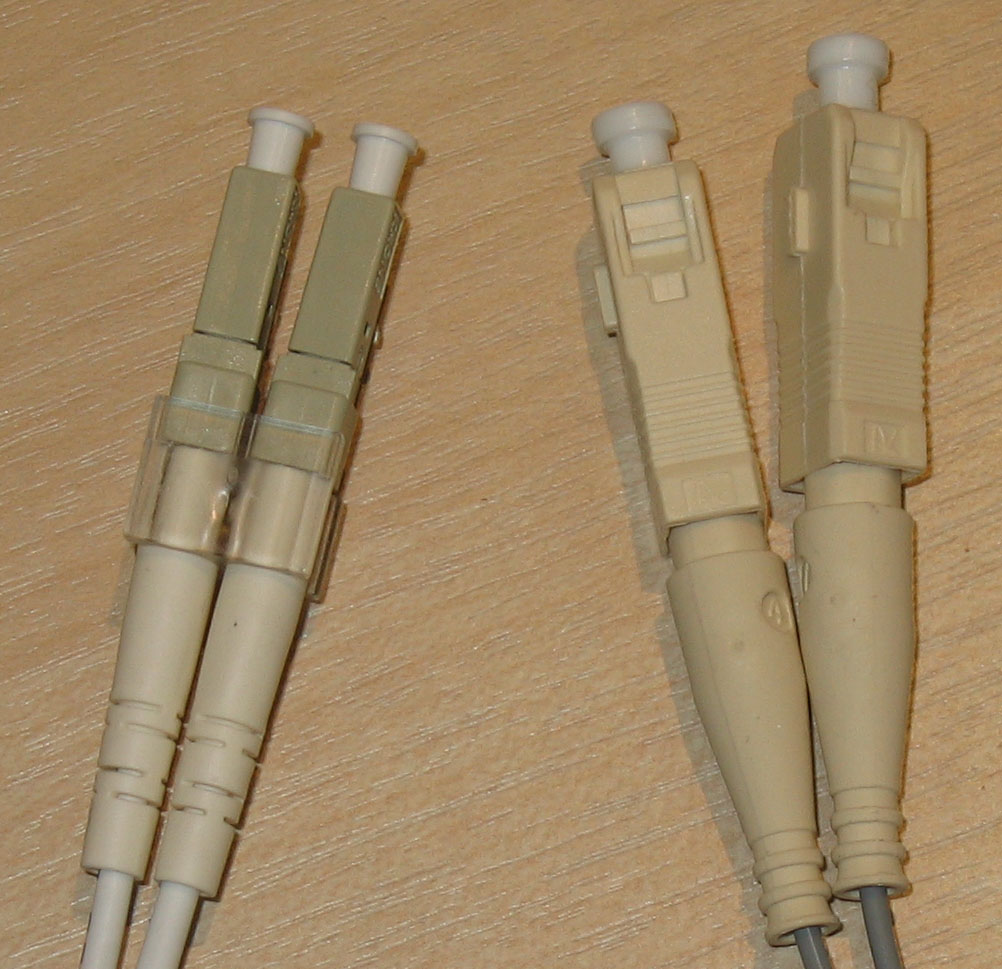
\includegraphics[keepaspectratio,alt={Connettori ottici LC (a sinistra) e SC (a destra) a confronto}]{images/Lc-sc-fiber-connectors-d94aa0.jpg}}
\emph{Fig. --- I connettori LC e SC sono i due standard dominanti per la
fibra ottica: LC per l'alta densità nei rack, SC per i cablaggi
metropolitani.}

\begin{callouttip}{La direzionalità della fibra ottica}

A differenza dei cavi in rame, un singolo filo di fibra ottica trasporta
la luce in una sola direzione. Per avere una comunicazione full-duplex è
sempre necessaria una \textbf{coppia di cavi}: uno per trasmettere (TX)
e uno per ricevere (RX). I connettori LC vengono spesso accoppiati
tramite una clip meccanica in plastica che può essere sfilata per
invertire i due connettori quando è necessario far coincidere
correttamente i canali TX e RX sui due estremi della connessione.

\end{callouttip}

\begin{center}\rule{0.5\linewidth}{0.5pt}\end{center}

\section{Cavi in Rame e Standard
Ethernet}\label{cavi-in-rame-e-standard-ethernet}

\subsection{Il Dominio del Rame}\label{il-dominio-del-rame}

Sebbene esistano reti dedicate all'HPC come \textbf{InfiniBand}, lo
standard Ethernet su cavi in rame ricopre ancora un ruolo dominante, con
oltre 70 miliardi di metri di cavo installati nel mondo. I moderni cavi
Ethernet utilizzano il connettore \textbf{RJ45}, che circa trent'anni fa
ha sostituito l'antico RJ11 telefonico. All'interno della guaina si
trovano 8 fili intrecciati a formare 4 coppie: le reti a 10 e 100
Megabit ne utilizzavano solo due, rendendo storicamente semplice il
passaggio a 1 Gigabit --- fu sufficiente abilitare le due coppie rimaste
inutilizzate all'interno dello stesso cavo.

L'assemblaggio manuale avviene inserendo i fili secondo uno schema
cromatico preciso all'interno del plug RJ45 e utilizzando una pressa
crimpatrice, che forza piccoli contatti metallici ``a lama'' a tagliare
la guaina dei singoli fili, stabilendo la connessione elettrica.

\pandocbounded{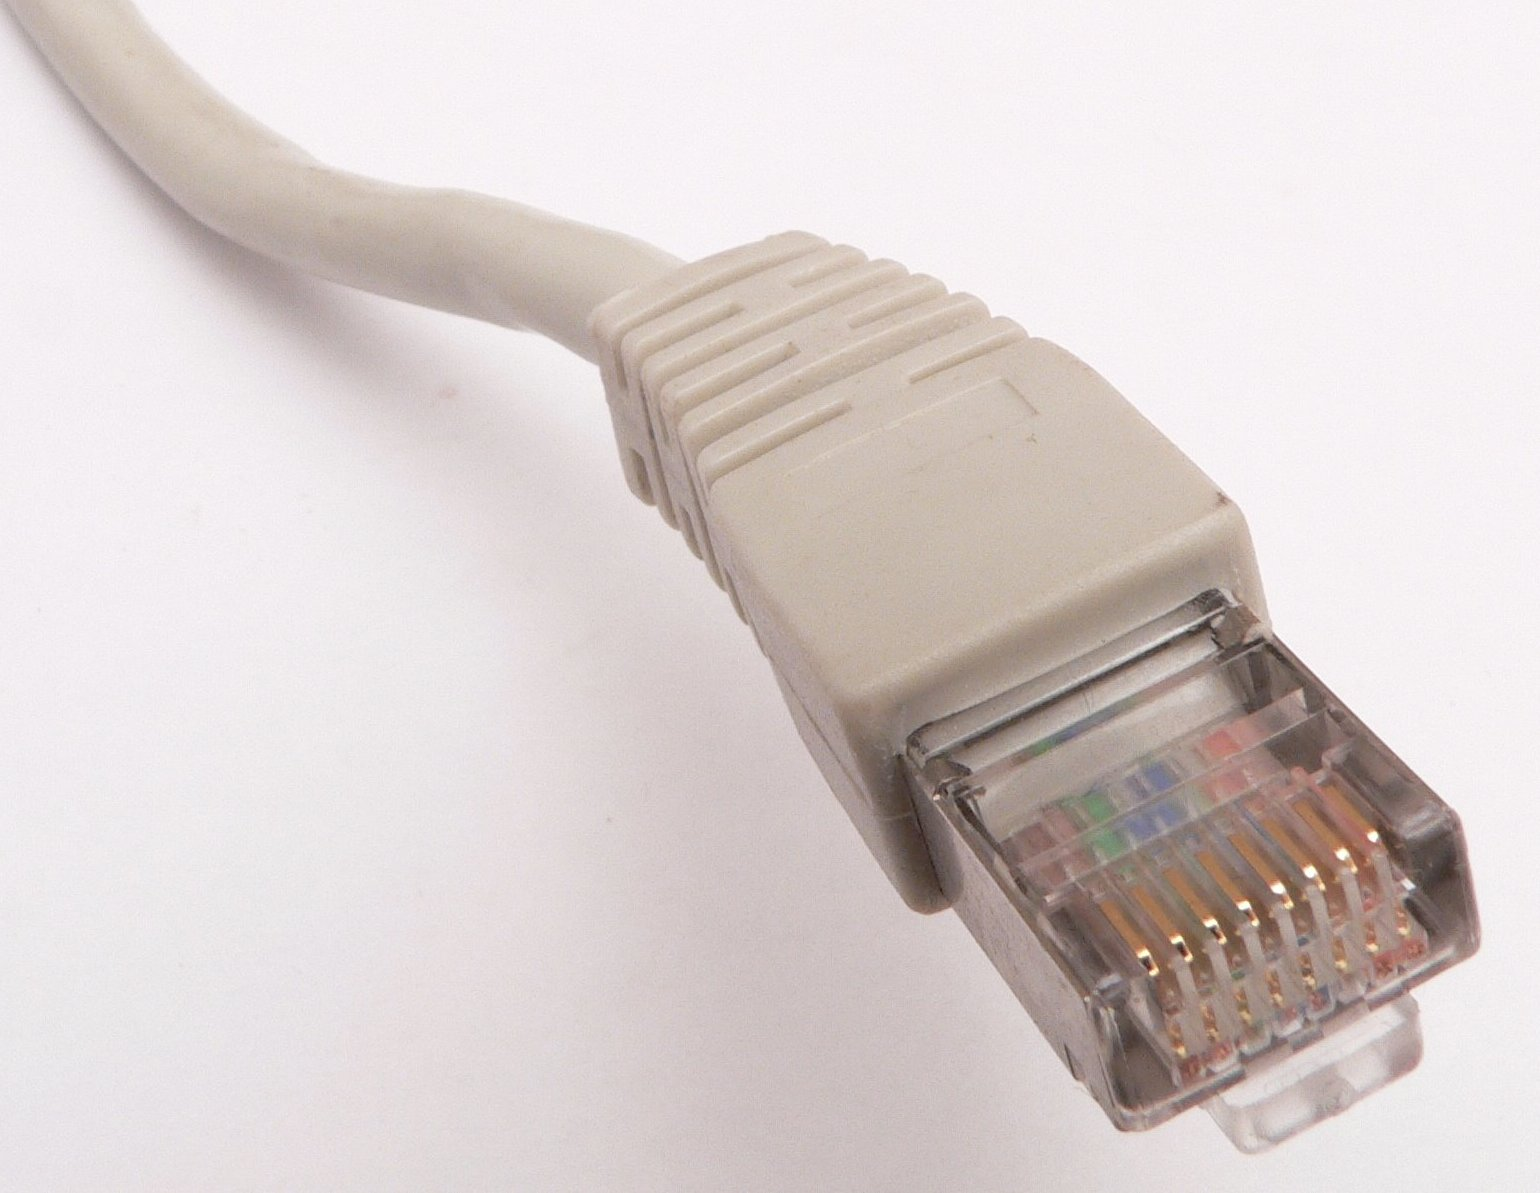
\includegraphics[keepaspectratio,alt={Connettore RJ45 Ethernet}]{images/Ethernet-RJ45-connector-p1160054-3256e0.jpg}}
\emph{Fig. --- Il connettore RJ45 con i suoi 8 pin; le 4 coppie di fili
intrecciati sono visibili all'interno della guaina.}

\subsection{La Sfida dei 10 Gigabit}\label{la-sfida-dei-10-gigabit}

Il superamento del muro di 1 Gigabit su rame si è rivelato una titanica
sfida ingegneristica, legata alle interferenze elettromagnetiche e alle
alte frequenze necessarie. La tabella seguente riassume l'evoluzione
degli standard:

{\def\LTcaptype{none} % do not increment counter
\begin{longtable}[]{@{}
  >{\raggedright\arraybackslash}p{(\linewidth - 6\tabcolsep) * \real{0.2500}}
  >{\raggedright\arraybackslash}p{(\linewidth - 6\tabcolsep) * \real{0.2500}}
  >{\raggedright\arraybackslash}p{(\linewidth - 6\tabcolsep) * \real{0.2500}}
  >{\raggedright\arraybackslash}p{(\linewidth - 6\tabcolsep) * \real{0.2500}}@{}}
\toprule\noalign{}
\begin{minipage}[b]{\linewidth}\raggedright
\textbf{Categoria}
\end{minipage} & \begin{minipage}[b]{\linewidth}\raggedright
\textbf{Capacità Max Pratica}
\end{minipage} & \begin{minipage}[b]{\linewidth}\raggedright
\textbf{Frequenza Max}
\end{minipage} & \begin{minipage}[b]{\linewidth}\raggedright
\textbf{Note}
\end{minipage} \\
\midrule\noalign{}
\endhead
\bottomrule\noalign{}
\endlastfoot
\textbf{Cat 5 / 5e} & 1 Gbps & 100 MHz & Standard storico e
diffusissimo \\
\textbf{Cat 6} & 1 Gbps (10G a corto raggio) & 250 MHz & Il più
installato; i 10G su Cat 6 sono sconsigliati \\
\textbf{Cat 6A} & 2.5 / 5 / 10 Gbps & 500 MHz & Massima evoluzione
pratica; raccomandato per i 10G in rame \\
\textbf{Cat 7 / Cat 8} & Oltre 10 Gbps & Oltre 600 MHz & Raramente
adottati; cavi estremamente spessi e rigidi \\
\end{longtable}
}

\begin{calloutwarning}{Il costo della ridondanza e i limiti del Cat 7/8}

Cat 7 e Cat 8 sono teoricamente disponibili ma praticamente
inutilizzabili: la rigidità dei cavi li rende simili a ``tubi di
ferro'', rendendo il cablaggio fisicamente impraticabile in ambienti
affollati. Sul piano economico, due cavi in rame ad alte prestazioni ---
necessari per garantire la ridondanza vitale di un server ed eliminare
il \emph{single point of failure} --- possono pesare sul budget fino a
300 dollari: un costo non trascurabile moltiplicato per centinaia di
server.

\end{calloutwarning}

\begin{center}\rule{0.5\linewidth}{0.5pt}\end{center}

\section{Gestione del Cablaggio}\label{gestione-del-cablaggio}

Gestire razionalmente il cablaggio (\emph{cable management}) non è una
questione estetica: è una necessità funzionale critica con impatto
diretto sull'efficienza energetica. La tendenza ad aggregare la
larghezza di banda ha portato ad avere fino a 4 cavi per server. In un
armadio contenente 30 server, ciò si traduce in oltre 120 cavi. Se si
aggiunge la prassi comune di ordinare cavi di lunghezze standard --- per
esempio 2 metri --- per uniformare il magazzino, il risultato è un
significativo accumulo di cavo in eccesso.

Se i cavi non vengono instradati in percorsi ordinati, formano una
barriera fisica sul retro del rack che ostruisce le bocchette di
estrazione dell'aria calda prodotta dai server. Il sistema di
raffreddamento rileva l'innalzamento anomalo delle temperature e
costringe le ventole ad accelerare drasticamente, con conseguente spreco
energetico e usura prematura dell'hardware. Il cablaggio disordinato, in
altre parole, degrada le prestazioni termiche dell'intero rack.

\begin{calloutnote}{Sintesi della lezione}

Il data center moderno è un sistema strettamente integrato in cui le
scelte di cablaggio, raffreddamento e distribuzione elettrica si
condizionano a vicenda. La transizione dal raffreddamento ad aria al
liquid cooling segue la crescita della densità di potenza per rack. La
fibra ottica è il medium di trasmissione dominante per distanze
superiori ai pochi metri, con la scelta tra monomodale e multimodale che
dipende dalla distanza e dal budget. Il rame rimane rilevante per i
collegamenti finali, ma Cat 6A è oggi il limite pratico oltre il quale
la fibra diventa obbligata. Il cable management, infine, non è un
dettaglio: un cablaggio disordinato degrada le prestazioni termiche
dell'intero rack.

\end{calloutnote}

\newpage

\chapter{Lezione 6 --- Fabric di un
Datacenter}\label{lezione-6-fabric-di-un-datacenter}

\section{Il Cablaggio Fisico nel Data
Center}\label{il-cablaggio-fisico-nel-data-center}

\subsection{Perché il cablaggio è una scelta
progettuale}\label{perchuxe9-il-cablaggio-uxe8-una-scelta-progettuale}

Quando si stende un cavo in un data center, non si esegue un'operazione
meccanica neutra: si sta prendendo una decisione architetturale. Il
cablaggio fisico determina la geometria della comunicazione tra i rack,
e quella geometria diventa poi un limite duro per le performance delle
applicazioni che girano sopra.

I motivi per cui il cablaggio è rilevante sono essenzialmente tre.

\textbf{Perdita di segnale.} Ogni connettore introdotto causa una
piccola attenuazione. All'interno del data center, dove i percorsi sono
brevi, questa perdita è trascurabile e non rappresenta un vincolo
pratico.

\textbf{Numero di hop.} Ogni switch attraversato da un pacchetto
introduce latenza. Un singolo switch Ethernet moderno introduce circa
\textbf{600 nanosecondi} di latenza. Sembra poco, ma ci sono workload
--- condivisione di memoria tra GPU, accesso a modelli AI distribuiti
--- in cui anche pochi microsecondidi aggiunta rendono il sistema
inutilizzabile.

\textbf{Flessibilità topologica.} La geometria del cablaggio determina
quanti percorsi fisici esistono tra due rack, quanto traffico est-ovest
può scorrere, e quanto è difficile riconfigurare la rete in caso di
aggiunta o rimozione di macchine.

\begin{callouttip}{La latenza end-to-end: il gap nascosto}

Un singolo switch Ethernet introduce \textasciitilde600 ns, ma appena si
sale al livello TCP/IP la latenza può arrivare a \textbf{70
microsecondi}. Per contesto: un accesso DRAM locale è nell'ordine dei
60--100 ns. Attraversare anche un solo hop TCP introduce una penalità
equivalente a centinaia di accessi in memoria. Per workload come i
modelli LLM distribuiti su GPU --- in lezione è citato GLM-4 con 750
miliardi di parametri in architettura Mixture of Experts --- questa
latenza diventa il collo di bottiglia dell'intero sistema.

\end{callouttip}

\subsection{Patch panel e zone
funzionali}\label{patch-panel-e-zone-funzionali}

Dato che non è pratico --- né riconfigurabile --- tirare cavi diretti da
ogni rack a ogni altro rack, la soluzione standard è il \textbf{patch
panel}: un pannello passivo che funge da punto di smistamento
intermedio, permettendo di ``teletrasportare'' logicamente una
connessione da una zona del data center all'altra semplicemente
spostando un cordone, senza rifare il cablaggio strutturale.

Il cablaggio strutturale presuppone una divisione in \textbf{zone
funzionali} del data center. Poiché collegare tutto con tutto è
fisicamente impraticabile (un grafo completo su N rack richiederebbe
\(\binom{N}{2}\) cavi), si assegnano ruoli alle aree: zona telco per i
link verso l'esterno, zone compute, zone storage, e così via.

\begin{calloutwarning}{Conseguenze di un cablaggio sbagliato}

Se la geometria del cablaggio non rispecchia il reale pattern di
comunicazione dei workload, i pacchetti saranno costretti a percorsi
subottimali: più hop, più latenza, meno banda. Questo si traduce in
limitazioni di performance visibili sulle VM, anche su cloud pubblici
come AWS o Azure --- sono il risultato diretto delle scelte fisiche
fatte da Microsoft o Amazon al momento dell'installazione del data
center.

\end{calloutwarning}

\subsection{Organizzazione fisica dei rack: pod e
corridoi}\label{organizzazione-fisica-dei-rack-pod-e-corridoi}

In un data center, i rack vengono tipicamente organizzati in \textbf{pod
di distribuzione}: insiemi di rack fisicamente adiacenti, disposti su
due file che si affacciano su un corridoio freddo confinato per il
raffreddamento. La prossimità fisica rende accettabile, in alcuni casi,
collegare rack adiacenti direttamente senza patch panel, eliminando le
pareti laterali dei rack e facendo passare i cavi internamente da un
rack al successivo.

La distinzione fondamentale rimane tra traffico \textbf{est-ovest}
(server-a-server all'interno del data center) e traffico
\textbf{nord-sud} (server verso l'esterno): hanno pattern e requisiti di
latenza radicalmente diversi, e ogni scelta di cablaggio li impatta in
modo diverso.

\begin{center}\rule{0.5\linewidth}{0.5pt}\end{center}

\section{I Transceiver: dal Cavo allo
Switch}\label{i-transceiver-dal-cavo-allo-switch}

\subsection{Il problema dei connettori
ottici}\label{il-problema-dei-connettori-ottici}

Quando le velocità di rete hanno superato la soglia in cui RJ45 e
doppino rame sono sufficienti, si è passati alla fibra ottica. Ma qui
emerge un problema economico: la fibra monomodale OS2 consente distanze
fino a \textbf{40 km}, ma all'interno di un data center non si superano
i 300 metri. Acquistare laser di potenza industriale pensati per decine
di chilometri è uno spreco enorme.

La soluzione è stata separare il trasmettitore ottico dallo switch
attraverso un \textbf{transceiver modulare}: un piccolo modulo attivo
che si inserisce in uno slot dedicato dello switch, converte il segnale
elettrico in ottico e viceversa, e determina il tipo di fibra, la
lunghezza d'onda e la distanza massima supportata.

\begin{calloutdefinition}{Transceiver (modulo SFP/QSFP)}

Modulo attivo hot-pluggable che si inserisce in uno slot del backplane
dello switch. Converte segnali elettrici in ottici e viceversa. Il
firmware del modulo espone allo switch le proprie caratteristiche
(velocità, tipo di fibra, range). Questo consente il \textbf{mix and
match}: slot 1 con fibra multimodale corto raggio, slot 3 con monomodale
lungo raggio, slot N con rame per debug --- tutto sullo stesso switch.

\end{calloutdefinition}

\subsection{La famiglia SFP: evoluzione degli
standard}\label{la-famiglia-sfp-evoluzione-degli-standard}

L'ecosistema dei transceiver si organizza intorno a famiglie
standardizzate. Conoscere questi nomi è competenza operativa
fondamentale in un data center.

\textbf{SFP28} è lo standard dominante per le porte server-facing nei
leaf switch. Supporta \textbf{25 Gbps} per lane e viene declinato in
varianti per distanza: \emph{SR (Short Range)} a 850 nm su fibra
multimodale per distanze fino a \textasciitilde100 m, \emph{LR (Long
Range)} a 1310 nm su fibra monomodale per distanze fino a
\textasciitilde10 km, e \emph{ER (Extended Range)} per portate ancora
maggiori.

Quando l'SFP28 ha raggiunto il suo limite fisico (la densità di segnale
non scalava oltre 25 Gbps con quel form factor), si è passati a
\textbf{QSFP} (\emph{Quad SFP}): stesso concetto ma con \textbf{4 lane
interne}. Le varianti della famiglia QSFP sono:

{\def\LTcaptype{none} % do not increment counter
\begin{longtable}[]{@{}llll@{}}
\toprule\noalign{}
Standard & Banda totale & Struttura interna & Note \\
\midrule\noalign{}
\endhead
\bottomrule\noalign{}
\endlastfoot
QSFP+ & 40 Gbps & 4×10G NRZ & Prima generazione \\
QSFP28 & 100 Gbps & 4×25G NRZ & Standard attuale per uplink
leaf↔spine \\
QSFP56 & 200 Gbps & 4×50G PAM4 & Uplink spine-to-spine \\
QSFP-DD & fino a 800 Gbps & 8×100G PAM4 & Ultima generazione, double
density \\
\end{longtable}
}

\begin{calloutnote}{Il salto a PAM4 e la logica dell’incremento}

Il passaggio da QSFP28 a QSFP56 non aumenta il numero di lane (rimangono
4), ma cambia la modulazione da NRZ a PAM4: invece di codificare 1 bit
per simbolo, PAM4 codifica 2 bit per simbolo, raddoppiando la banda a
parità di frequenza. Il QSFP-DD raddoppia ulteriormente le lane da 4 a
8, mantenendo le stesse dimensioni fisiche esterne ma con una scheda di
contatti più profonda.

\end{calloutnote}

\subsection{Codici colore e decodifica del
modulo}\label{codici-colore-e-decodifica-del-modulo}

I transceiver usano \textbf{codici colore} convenzionali: il blu
identifica tipicamente la fibra monomodale, il nero o grigio la
multimodale. Sul corpo del modulo è inciso il codice completo: tipo (es.
SFP28), velocità (25G), lunghezza d'onda (850 nm → multimodale, 1310 nm
→ monomodale), range (SR/LR/ER).

\textbf{Perché la multimodale domina il data center?} Perché le distanze
interne raramente superano i 100--300 metri, e la fibra multimodale è
significativamente più economica sia nei cavi che nei laser. In lezione
è stato fatto un confronto pratico: un modulo SFP28 SR (multimodale)
costa circa €45; ne servono due (uno per estremo) più il cavo ottico
(\textasciitilde€10), per un totale di \textasciitilde€100. Un cavo DAC
(\emph{Direct Attach Cable}) in rame ha un costo simile, ma la soluzione
a transceiver offre modularità: si sostituiscono i moduli per aggiornare
la velocità senza cambiare il cavo.

\begin{callouttip}{Evoluzione della banda per transceiver nel tempo}

2005: 1 Gbps → 2010: 10 Gbps → 2015: 25--40 Gbps → 2020: 100--200 Gbps →
2024: 400--800 Gbps. In vent'anni, un fattore 800×. Ogni generazione ha
richiesto nuovi form factor e nuovi laser, ma il principio di modularità
degli slot è rimasto invariato.

\end{callouttip}

\begin{center}\rule{0.5\linewidth}{0.5pt}\end{center}

\section{Gli Switch: dai Chassis Modulari al Form Factor
Fisso}\label{gli-switch-dai-chassis-modulari-al-form-factor-fisso}

\subsection{L'era dei chassis}\label{lera-dei-chassis}

Fino ai primi anni 2000, lo switch tipico di un data center era un
\textbf{chassis modulare}: un armadio di grandi dimensioni nel quale si
inserivano \emph{line card} --- schede con più porte Ethernet --- e un
modulo \textbf{RPM} (\emph{Routing Processing Module}) responsabile del
coordinamento attraverso un \emph{backplane} condiviso.

Questi switch erano costosissimi, quindi tipicamente un data center ne
aveva \textbf{due} per ridondanza, e tutti i cavi del data center
confluivano verso questi due switch centrali. Da questa architettura
fisica nacque naturalmente una topologia a stella: un unico punto di
smistamento centrale attorno al quale tutto era organizzato.

\begin{calloutnote}{Eredità nella nomenclatura delle porte}

La notazione \texttt{X/Y} delle porte Ethernet (es. \texttt{0/1} =
\emph{line card 0, porta 1}) è una diretta eredità della struttura
bidimensionale del chassis. Sugli switch moderni a form factor fisso non
esiste più la line card, ma la convenzione è rimasta in tutto il
software di gestione di rete.

\end{calloutnote}

\subsection{La crisi del backplane e la
transizione}\label{la-crisi-del-backplane-e-la-transizione}

Il modello a chassis aveva senso economico finché la banda cresceva
lentamente. Ma quando la velocità Ethernet ha cominciato a raddoppiare
ogni pochi anni --- da 1G a 10G a 25G --- il \textbf{backplane} del
chassis non riusciva più a stare al passo. Progettare un backplane
capace di supportare la velocità attuale significava che tra due anni
sarebbe già obsoleto, e il chassis costoso acquistato aveva già schede
mezze vuote.

La risposta è stata la transizione agli \textbf{switch a form factor
fisso}: switch compatti, tipicamente 1U, con un numero fisso di porte,
montabili direttamente top-of-rack. Questi switch sono più economici,
più facili da sostituire, e avvicinano il punto di switching ai server
riducendo la lunghezza dei cavi e il numero di hop.

\begin{center}\rule{0.5\linewidth}{0.5pt}\end{center}

\section{Topologia di Rete: da 3-Tier a
Spine-and-Leaf}\label{topologia-di-rete-da-3-tier-a-spine-and-leaf}

\subsection{Architettura 3-tier}\label{architettura-3-tier}

Il concentrare lo switching in pochi chassis centrali produsse la
topologia \textbf{3-tier}: \emph{access layer} vicino ai server,
\emph{distribution layer} di aggregazione intermedia, \emph{core layer}
con i grandi chassis centrali. Tutto il traffico doveva passare per il
core. Questo era accettabile finché il traffico dominante era nord-sud.

\pandocbounded{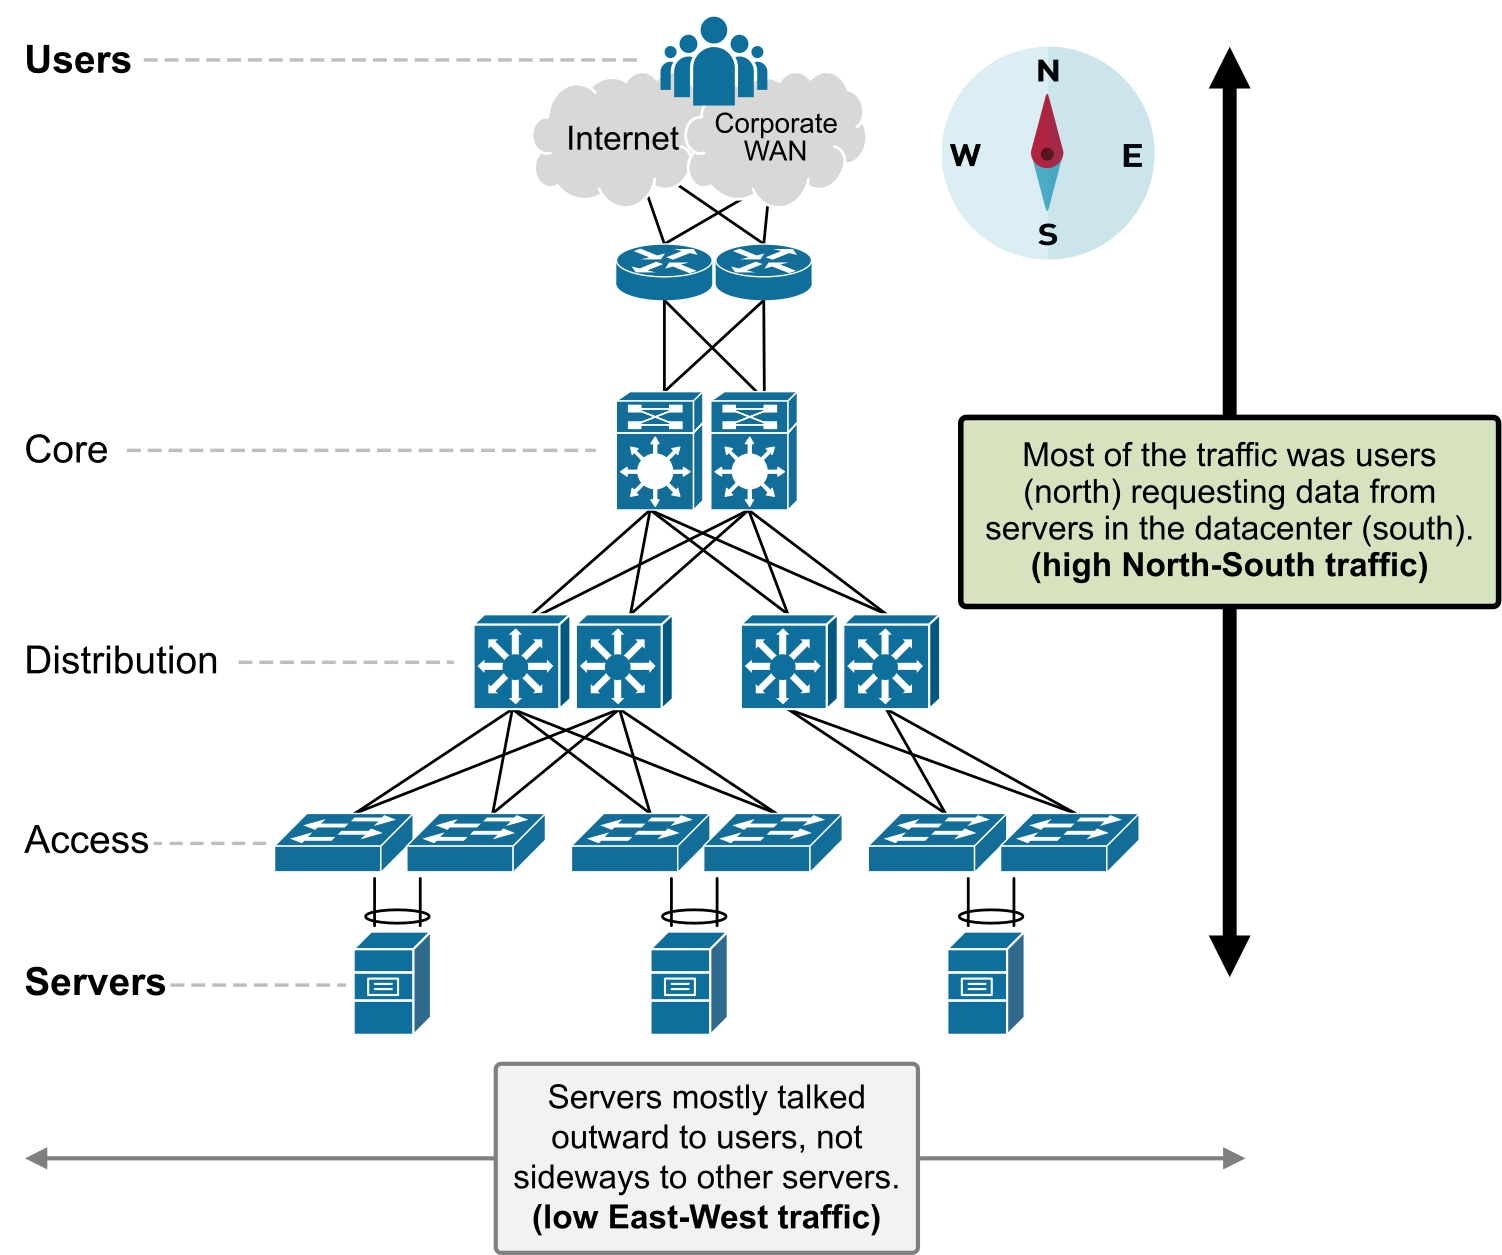
\includegraphics[keepaspectratio,alt={Traffico nord-sud nell'architettura 3-tier}]{images/three-tier-architecture-traffic-5d3d84.png}}
\emph{Fig. 1 --- In architettura 3-tier il traffico tipico è nord-sud: i
client accedono ai server dall'esterno. Core e distribution switch
gestiscono questi flussi in modo efficiente.}

Con l'avvento dei microservizi, del cloud e dell'AI, il traffico
est-ovest è diventato dominante: ogni richiesta applicativa coinvolge
decine di servizi che si parlano tra loro all'interno del data center.

\pandocbounded{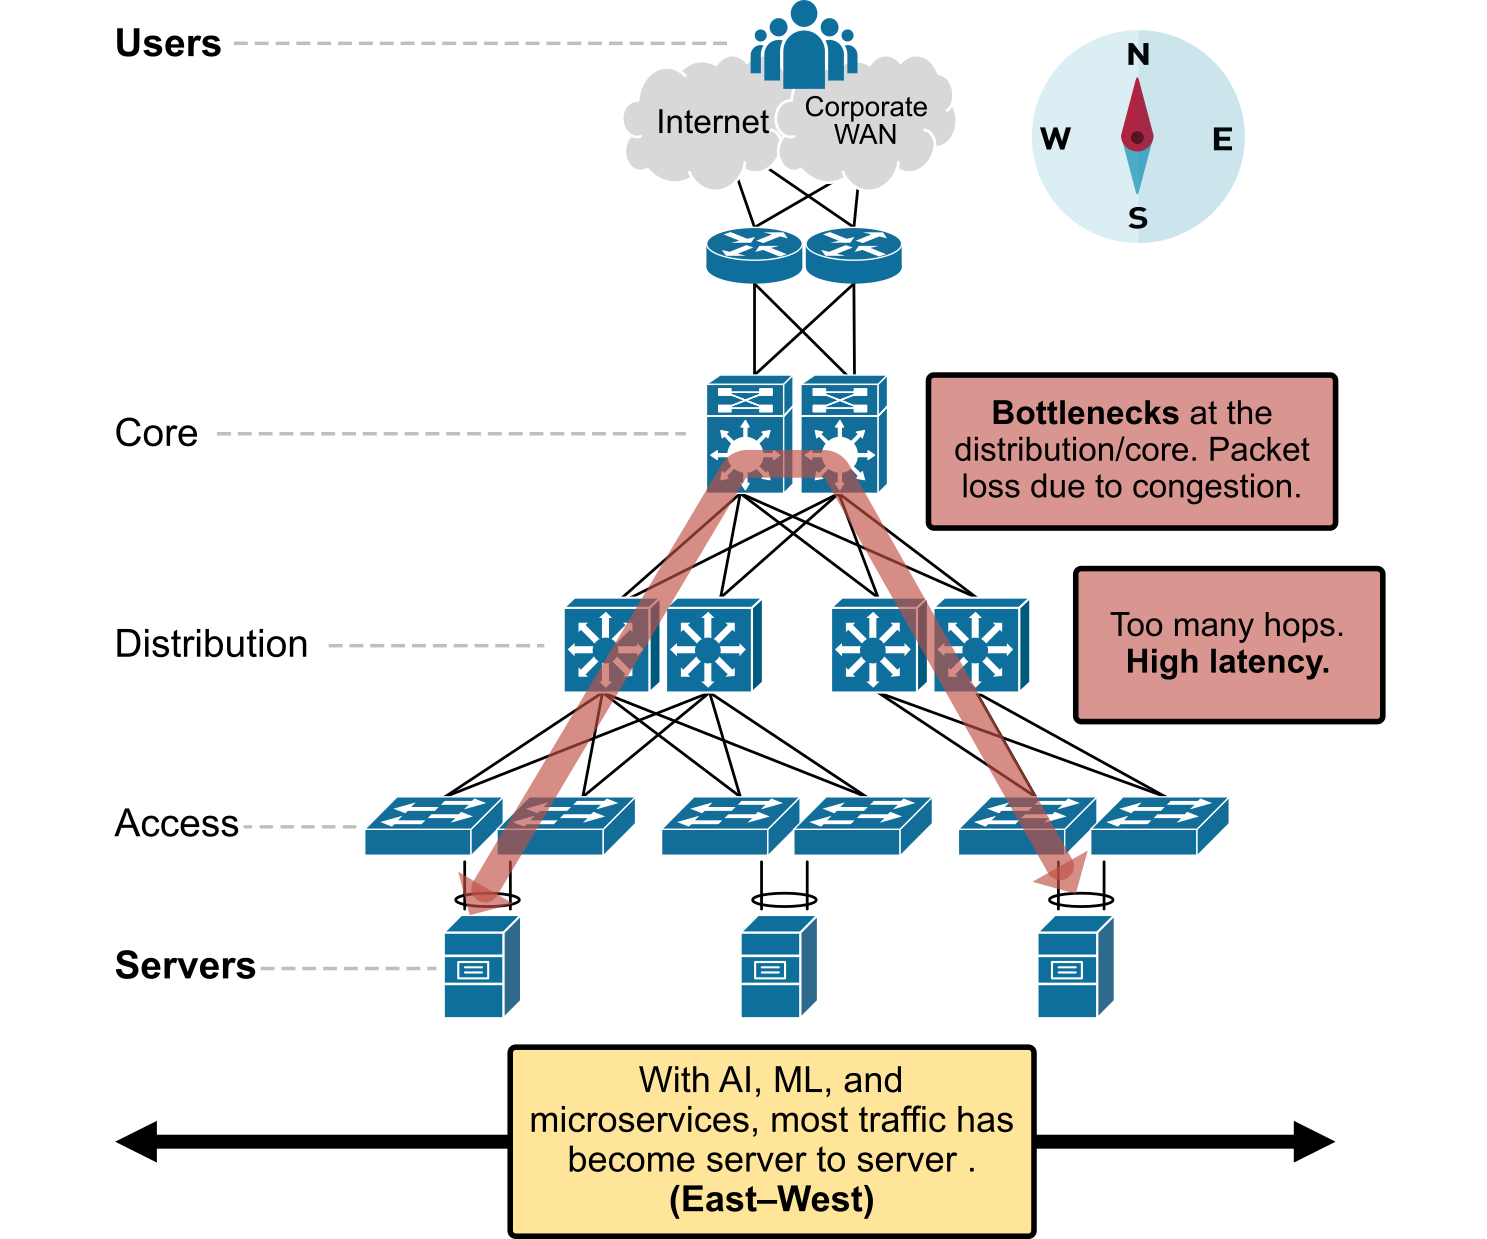
\includegraphics[keepaspectratio,alt={Inefficienze della 3-tier con traffico est-ovest}]{images/three-tier-inefficiencies-a922f0.png}}
\emph{Fig. 2 --- Con traffico east-west dominante, ogni comunicazione
server-a-server deve risalire access → distribution → core →
distribution → access: latenza variabile, colli di bottiglia sugli
uplink.}

\subsection{STP: soluzione necessaria ma
costosa}\label{stp-soluzione-necessaria-ma-costosa}

Per garantire ridondanza occorrono percorsi fisici multipli, ma più
percorsi creano loop in Ethernet.

\begin{calloutwarning}{Loop e broadcast storm}

In Ethernet, un loop causa un \textbf{broadcast storm}: un frame
broadcast rimbalza all'infinito amplificandosi, satura tutta la banda e
rende la rete inutilizzabile in pochi secondi. È un problema concreto
che si presenta ogni volta che un cavo crea accidentalmente un ciclo
nella topologia.

\end{calloutwarning}

\begin{calloutdefinition}{Spanning Tree Protocol (STP / RSTP)}

Protocollo di livello 2 (IEEE 802.1D / 802.1W) che costruisce
dinamicamente un albero di copertura della rete, \textbf{disabilitando i
link che formerebbero cicli}. In caso di guasto di un link attivo,
ricalcola l'albero e riabilita un link precedentemente disabilitato. STP
converge in decine di secondi; RSTP in qualche secondo.

\end{calloutdefinition}

\pandocbounded{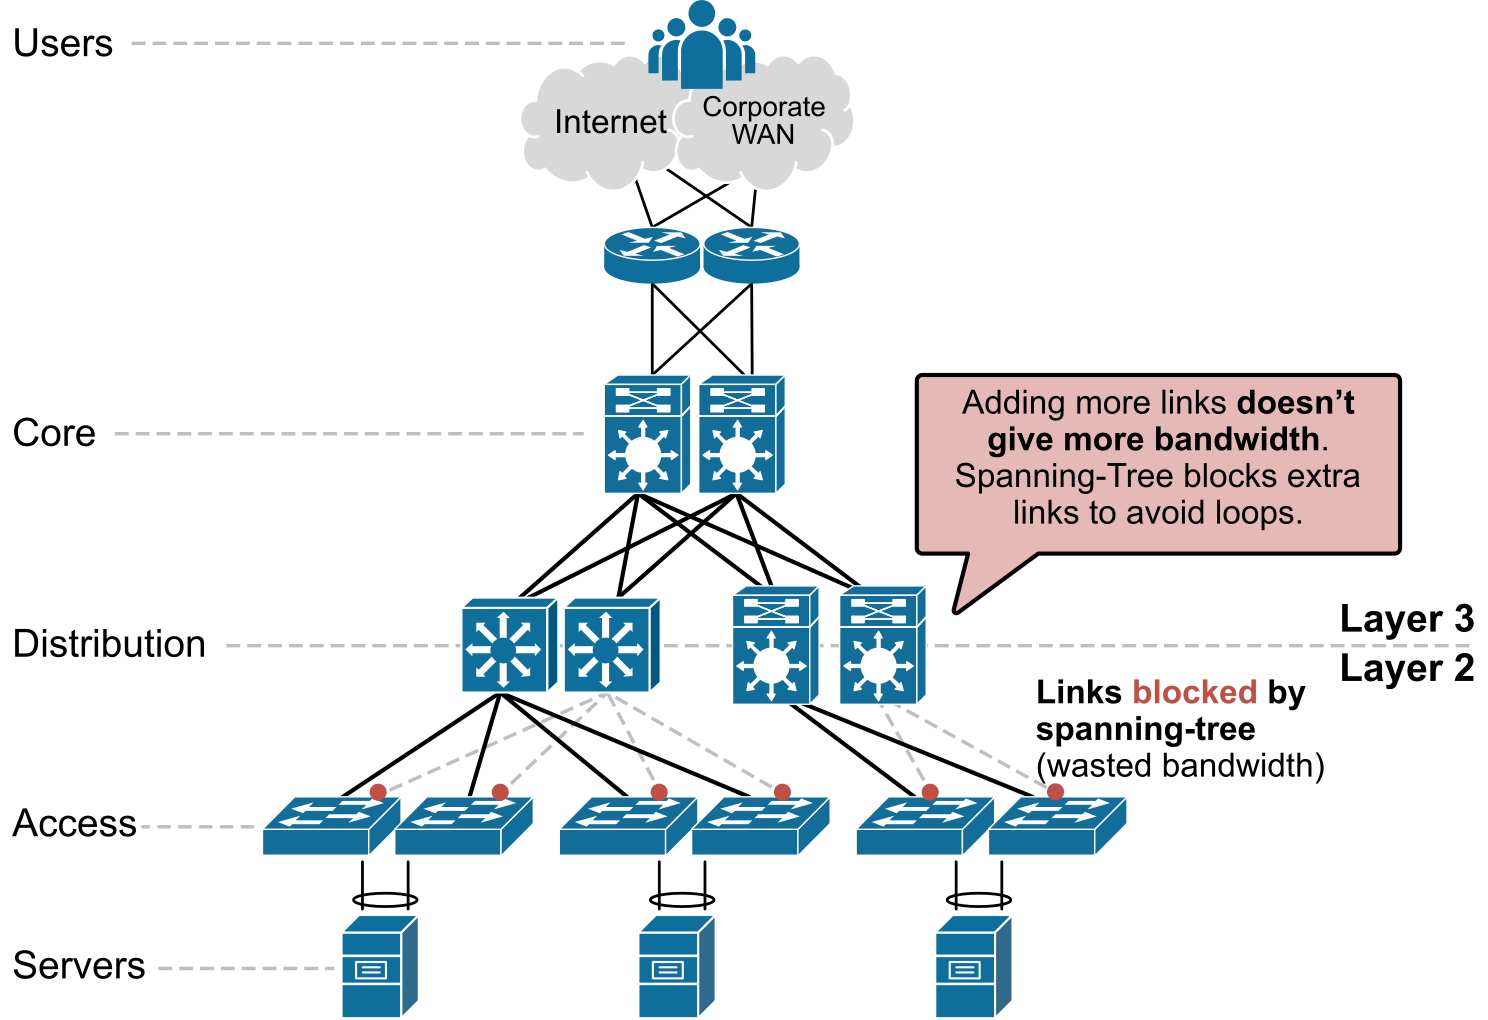
\includegraphics[keepaspectratio,alt={STP blocca i link ridondanti nella topologia 3-tier}]{images/three-tier-spanning-tree-fa1cb3.png}}
\emph{Fig. 3 --- STP in azione: i link ridondanti (tratteggiati/rossi)
vengono disabilitati per eliminare i loop. Il cavo fisico è presente e
pagato, ma non trasporta traffico.}

Il costo di STP è duplice. Primo: \textbf{spreco di risorse} --- il link
ridondante è fisicamente presente e pagato (cavo, transceiver, porta
dello switch), ma non trasporta traffico. Secondo: \textbf{lentezza di
convergenza} --- STP originale impiega fino a \textbf{50 secondi} per
convergere dopo un guasto, RSTP qualche secondo. Un'interruzione di 50
secondi è accettabile per traffico web a basso carico; è un disastro se
il fabric collega VM alle proprie unità di storage virtuali (la VM
perderebbe il disco per tutta la durata).

\subsection{Spine-and-Leaf: la topologia dominante
oggi}\label{spine-and-leaf-la-topologia-dominante-oggi}

\begin{calloutdefinition}{Spine-and-Leaf}

Topologia di rete a due livelli in cui i \textbf{leaf switch} raccolgono
i server (tipicamente top-of-rack, uno per rack) e i \textbf{spine
switch} interconnettono i leaf. Ogni leaf è collegato a ogni spine,
producendo un grafo bipartito regolare. Il cammino tra qualsiasi coppia
di server è costante: leaf → spine → leaf, ovvero \textbf{2 hop fisici,
1 hop logico}.

\end{calloutdefinition}

I leaf switch non si parlano mai direttamente: tutto il traffico
est-ovest passa obbligatoriamente per uno spine. Questo garantisce
latenza \textbf{uniforme e predicibile} indipendentemente da dove si
trovano i due server.

\pandocbounded{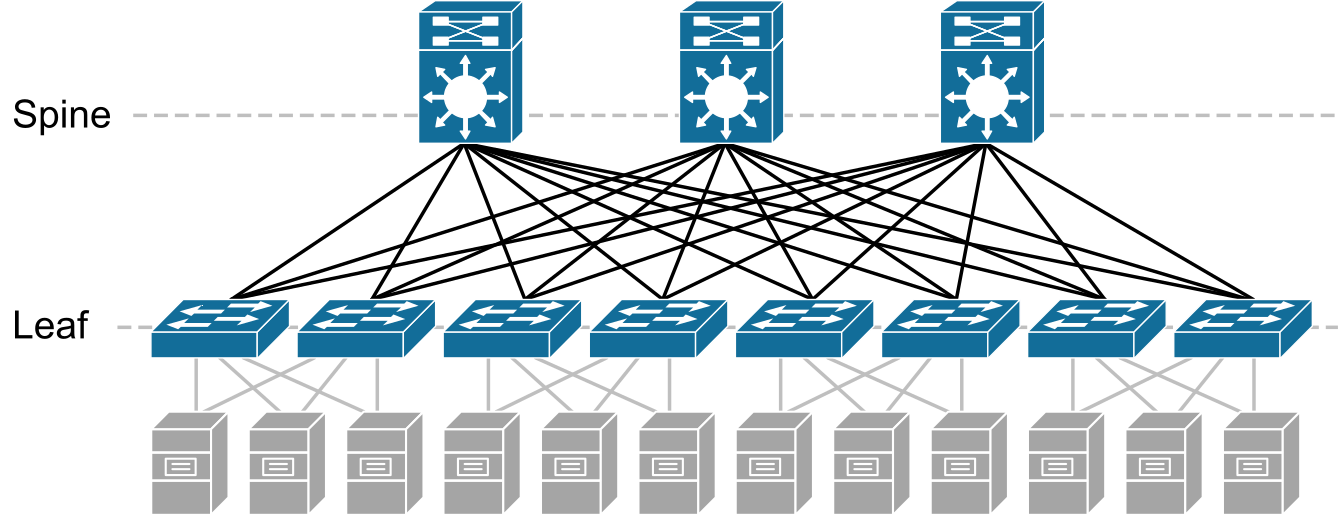
\includegraphics[keepaspectratio,alt={Architettura spine-and-leaf}]{images/leaf-spine-architecture-919c04.png}}
\emph{Fig. 4 --- Spine-and-leaf: ogni leaf si connette a tutti gli
spine. Qualunque comunicazione server-a-server attraversa esattamente
uno spine, con latenza costante. Aggiungere capacità significa
aggiungere leaf (scale-out orizzontale).}

\subsection{Ridondanza senza STP: link aggregation
active-active}\label{ridondanza-senza-stp-link-aggregation-active-active}

Con spine-and-leaf la ridondanza si ottiene tramite \textbf{link
aggregation}: due spine switch fisicamente distinti vengono fatti
operare come un singolo switch logico (tramite protocolli come vPC di
Cisco, MLAG di Arista, o il protocollo standard LACP). Ogni leaf vede
due cavi verso lo spine ma li tratta come un'unica interfaccia logica ad
alta banda. Lo schema è \textbf{active-active}: entrambi i link
trasportano traffico contemporaneamente.

\begin{callouttip}{Aggregazione di banda con spine pair}

Se ogni link leaf↔spine è da 25 Gbps, aggregando due spine si hanno 50
Gbps di banda disponibile tra un leaf e lo strato spine. Un singolo
stream TCP rimane limitato a 25 Gbps (non si può dividere un flusso su
due link), ma due stream paralleli possono usare link diversi, sommando
a 50 Gbps totali. Se uno spine cade, la banda degrada da 50 a 25 Gbps ma
la connettività non si interrompe --- nessun STP da aspettare.

\end{callouttip}

\subsection{Confronto 3-tier vs
Spine-and-Leaf}\label{confronto-3-tier-vs-spine-and-leaf}

{\def\LTcaptype{none} % do not increment counter
\begin{longtable}[]{@{}lll@{}}
\toprule\noalign{}
Dimensione & 3-tier / Chassis & Spine-and-Leaf \\
\midrule\noalign{}
\endhead
\bottomrule\noalign{}
\endlastfoot
Latenza & Variabile (dipende dal path) & Fissa e bassa (1 hop logico) \\
Banda & Limitata dalla gerarchia & Aggregata e scalabile \\
Link ridondanti & Disabilitati da STP (sprecati) & Attivi ---
active-active \\
Traffico est-ovest & Subottimale & Nativo e ottimizzato \\
Convergenza dopo guasto & Secondi (RSTP) & Istantanea (degradazione
banda) \\
Scalabilità & Verticale (upgrade chassis) & Orizzontale (aggiungere
leaf) \\
\end{longtable}
}

\begin{calloutnote}{Perché spine-and-leaf ha vinto}

Tre ragioni sintetizzano il dominio di spine-and-leaf nei data center
moderni. Prima: \textbf{latenza a 1 hop} --- qualunque server raggiunge
qualunque altro con latenza predicibile. Seconda: \textbf{banda
aggregata} --- nessun costo per link inutilizzati, tutto l'hardware
lavora. Terza: \textbf{east-west friendly} --- il traffico interno al
data center, fondamentale per microservizi, storage distribuito e GPU
cluster AI, non deve più risalire gerarchie di switch lente.

\end{calloutnote}

\begin{center}\rule{0.5\linewidth}{0.5pt}\end{center}

\section{Data Center vs Campus
Network}\label{data-center-vs-campus-network}

Spine-and-leaf è pensata per il traffico \textbf{est-ovest} dominante
nei data center. Nelle \textbf{reti campus} --- università, uffici, reti
Wi-Fi --- il traffico è prevalentemente \textbf{nord-sud}: gli utenti
accedono a risorse esterne. Per questo le reti campus continuano a usare
architetture gerarchiche tipo 3-tier con STP: la convergenza lenta è
accettabile, e lo spreco dei link ridondanti non è critico.

\begin{calloutnote}{La rete Wi-Fi del campus}

La rete wireless universitaria è un'architettura north-south, non
spine-leaf. Questo spiega perché in Wi-Fi spesso non si riesce a pingare
altri dispositivi collegati alla stessa access point: il traffico non è
ottimizzato per la comunicazione laterale.

\end{calloutnote}

\begin{center}\rule{0.5\linewidth}{0.5pt}\end{center}

\section{Conclusioni e Punti Chiave}\label{conclusioni-e-punti-chiave}

Questa lezione ha tracciato il percorso dal cavo fisico all'architettura
di rete, mostrando come ogni scelta a basso livello si rifletta in
caratteristiche osservabili ad alto livello. Capire queste scelte
fisiche è essenziale per comprendere perché una VM su AWS ha certi
limiti di banda, o perché un'applicazione distribuita su rack diversi si
comporta diversamente da una co-locata sullo stesso rack.

Il corso proseguirà con le infrastrutture \textbf{convergenti e
iperconvergenti} --- tecnologie che dipendono direttamente dalla
capacità del fabric spine-and-leaf di gestire traffico est-ovest con
latenza controllata e banda prevedibile.

\begin{quote}
\begin{itemize}
\tightlist
\item
  In quale contesto si usa ancora un'architettura 3-tier? Perché è
  accettabile lì ma non in un data center?
\end{itemize}
\end{quote}

\newpage

\chapter{Lezione 7 --- Switching}\label{lezione-7-switching}

\section{Il Contesto: Perché il Network è
Cambiato}\label{il-contesto-perchuxe9-il-network-uxe8-cambiato}

Per capire l'architettura attuale degli switch è necessario capire
\emph{perché} è cambiata rispetto al passato. Il docente traccia una
periodizzazione sintetica ma illuminante dell'evoluzione dei workload in
ambito IT.

Per quasi tre decenni, il panorama applicativo era diviso in due
categorie: l'\textbf{HPC} (High Performance Computing), dove il calcolo
superava la capacità del singolo nodo e si ricorreva a cluster, e le
\textbf{applicazioni enterprise} --- web server, database, middleware
--- dove la capacità di calcolo disponibile superava di gran lunga
quanto necessario e si preferiva concentrare più servizi su un singolo
nodo denso di core. In entrambi i casi, la rete era un fattore
secondario: le applicazioni enterprise vivevano prevalentemente di
traffico Nord-Sud (client verso server), mentre in HPC i nodi
comunicavano su interconnessioni specializzate.

Tutto cambia intorno al \textbf{2013}, con l'esplosione del paradigma
Big Data (Hadoop e simili). L'adozione massiva di SSD, che abbassano la
latenza di accesso allo storage da millisecondi a microsecondi, rende
conveniente muovere grandi quantità di dati all'interno del data center.
Nasce così il cosiddetto traffico \textbf{East-West}: comunicazione da
server a server all'interno dello stesso datacenter. Questo tipo di
traffico esige reti a bassa latenza e alta banda tra i nodi, requisiti
molto diversi rispetto al traffico tradizionale.

Il colpo finale al vecchio ordine arriva con l'\textbf{AI generativa}.
Per la prima volta emerge un workload che richiede simultaneamente:
molto calcolo, molta memoria veloce, molte GPU e interconnessioni ad
altissima banda. Il bilanciamento del sistema si rompe, e tutti i
componenti --- CPU, memoria, storage, rete --- devono essere ripensati.

\begin{callouttip}{Il principio del bilanciamento}

Un sistema è efficiente solo quando tutti i suoi componenti sono
dimensionati in modo coerente. Avere una rete da 200 Gbps con CPU che
processano al massimo 80 Gbps è uno spreco. La progettazione del data
center è sempre un esercizio di bilanciamento.

\end{callouttip}

\subsection{La Fine dei Chassis e il Fixed Form
Factor}\label{la-fine-dei-chassis-e-il-fixed-form-factor}

Sul lato networking, un ulteriore cambiatore è stata la velocità di
evoluzione della tecnologia. In passato era conveniente investire in
chassis modulari costosi (uno switch chassis con schede sostituibili),
poiché la vita utile dell'investimento era lunga. Ma quando la capacità
dei port ASIC raddoppia ogni pochi anni, il chassis diventava obsoleto
prima delle sue schede. Il costo di un chassis a lunga vita non si
giustificava più.

La risposta è stata il \textbf{fixed form factor switch}: 1 o 2 unità
rack, non modulare, ma aggregabile via software in topologie spine-leaf.
Questo approccio rende il traffico East-West più prevedibile --- sia in
latenza che in banda --- e consente di aggiornare la rete sostituendo
interi switch (commodity hardware) invece di investire in chassis
proprietari.

\begin{center}\rule{0.5\linewidth}{0.5pt}\end{center}

\section{Architettura Interna dello
Switch}\label{architettura-interna-dello-switch}

Uno switch moderno da data center non è un appliance speciale: è
fondamentalmente un \textbf{computer general purpose} a cui è stato
affiancato hardware specializzato per il forwarding dei pacchetti. Il
professore insiste su questo punto perché rompe la percezione comune
dello switch come ``scatola nera'' di rete.

\begin{calloutdefinition}{Control Plane e Data Plane}

Lo \textbf{switch di rete} --- come qualsiasi dispositivo di
comunicazione complesso --- si divide in due piani funzionali distinti:

\begin{itemize}
\tightlist
\item
  Il \textbf{Control Plane} (piano di controllo) è responsabile della
  \emph{configurazione}, della \emph{gestione} e del
  \emph{monitoraggio}. Qui risiedono la logica delle policy, i
  protocolli di routing, i contatori delle porte, il sistema operativo
  di rete.
\item
  Il \textbf{Data Plane} (piano dati) è responsabile
  dell'\emph{esecuzione}: riceve i pacchetti sulle porte ingress,
  determina la porta egress consultando le tabelle popolate dal control
  plane, e li instrada alla velocità del silicio.
\end{itemize}

\end{calloutdefinition}

\pandocbounded{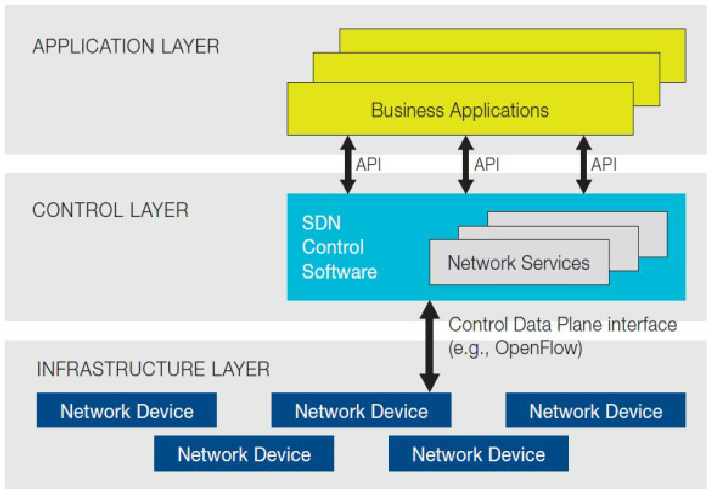
\includegraphics[keepaspectratio,alt={Architettura SDN: separazione tra application layer, control plane e data plane (infrastructure layer)}]{images/Software-defined-networking-SDN-architecture-source-Open-Networking-Foundation-ONF1-36c6af.png}}
\emph{Fig. --- La separazione funzionale tra i piani di rete secondo
l'Open Networking Foundation: application layer (policy e gestione),
control plane (logica di routing) e infrastructure layer (forwarding a
linerate nel silicio). Nello switch da data center moderno il management
coincide tipicamente con il control plane.}

\subsection{Il Data Plane: Silicon
Commodity}\label{il-data-plane-silicon-commodity}

Il data plane è dove si esegue il vero lavoro di forwarding, e oggi è
dominato da \textbf{ASIC} (Application-Specific Integrated Circuit)
forniti da un numero ristretto di vendor. Broadcom è il nome più citato
in questo settore: chip come il \textbf{Jericho} sono progettati per
memorizzare la tabella di routing completa dell'Internet pubblico (e il
doppio, stando alle specifiche) e per forwarding a linerate di terabit
per secondo. Chiunque voglia costruire uno switch compra il catalogo
Broadcom, sceglie il chip in base alle prestazioni desiderate e progetta
la scheda attorno ad esso.

Questo ha una conseguenza fondamentale: \textbf{il data plane è
diventato commodity}. La differenziazione tra vendor non sta più nel
silicio ma nel software del control plane e nell'ecosistema di gestione.

\begin{calloutnote}{Non-blocking switching}

Uno switch si dice \textbf{non-blocking} quando può commutare
simultaneamente tutto il traffico su tutte le sue porte senza che nessun
flusso debba aspettare. Con 48 porte da 25 Gbps + 8 uplink da 100 Gbps,
il backplane deve reggere:
\((48 \times 25 + 8 \times 100) \times 2 = 3.6 \text{ Tbps}\) Il fattore
\(\times 2\) è perché ogni porta lavora in full-duplex (RX + TX). Gli
switch da data center moderni sono progettati per essere non-blocking, e
il costo di questa capacità si riflette nell'alimentazione: sono
macchine da 700 W, contro i 200 W di una volta.

\end{calloutnote}

\subsection{Il Control Plane: Linux dentro lo
Switch}\label{il-control-plane-linux-dentro-lo-switch}

Al di sopra del data plane c'è il control plane, che è ---
sorprendentemente per chi non ci ha mai lavorato --- un \textbf{Linux}
che gira su una CPU Intel Celeron o equivalente. Ci sono RAM, storage
flash, e una connessione PCIe verso l'ASIC del data plane. Il bus PCIe
in uno switch non ha la stessa larghezza di banda di quello di un
server: la sua funzione è inviare comandi di configurazione all'ASIC
(aggiornare le tabelle di forwarding, cambiare le policy delle porte),
non trasportare i dati dei pacchetti.

\begin{calloutwarning}{PCIe tra control e data plane: non è una pipe di dati}

Il bus PCIe che collega control plane e data plane in uno switch è
dimensionato per la \emph{configurazione}, non per il \emph{forwarding}.
In linea di principio si potrebbero far processare i pacchetti dalla CPU
del control plane, ma la banda disponibile non è sufficiente per reggere
il volume di traffico che l'ASIC gestisce. Questo limita il tipo di
funzioni implementabili nel software rispetto all'hardware.

\end{calloutwarning}

\begin{center}\rule{0.5\linewidth}{0.5pt}\end{center}

\section{SONiC e l'Open Networking}\label{sonic-e-lopen-networking}

Il fatto che il silicio sia commodity ha aperto la porta alla
disaggregazione hardware/software, un trend che in ambito server è
avvenuto decenni fa (BIOS + OS generico) e che nella rete stava tardando
per ragioni miste: tecniche e commerciali.

\textbf{ONIE} (Open Network Install Environment) è il bootloader
standard per switch che supporta questa disaggregazione. Esattamente
come GRUB carica un OS su un PC, ONIE carica un'immagine di Network
Operating System sullo switch. Chi compra uno switch ONIE-compatibile
può scegliere quale NOS installare, come si fa con un server.

\textbf{SONiC} (Software for Open Networking in the Cloud) è il NOS open
source sviluppato originariamente da Microsoft per i propri data center
Azure e poi donato alla comunità tramite la Linux Foundation. È
costruito su Linux, basato su container Docker per la modularità, e
utilizza Redis come database in-memory per la comunicazione tra i
componenti. Oggi è co-mantenuto da Microsoft, Arista, Dell e molti altri
vendor.

\pandocbounded{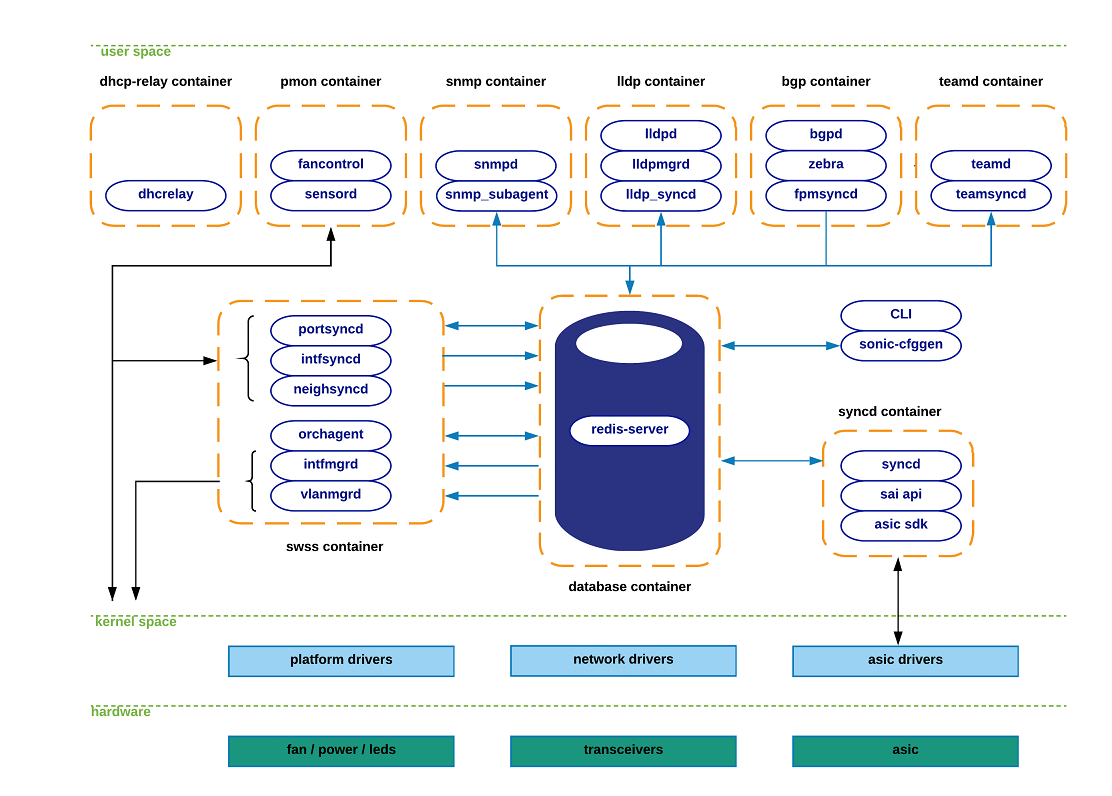
\includegraphics[keepaspectratio,alt={SONiC --- architettura ad alto livello con componenti containerizzati}]{images/TAHKyAT-6370ad.png}}
\emph{Fonte: Azure/SONiC (GitHub) --- Architettura di SONiC: ogni
funzione di rete (BGP, LLDP, SNMP, DHCP relay) gira in un container
Docker separato e comunica tramite Redis DB.}

\begin{calloutnote}{Due immagini OS sullo switch}

Gli switch moderni mantengono due immagini del sistema operativo sul
disco: quella \emph{corrente} in esecuzione e una di \emph{riserva}.
Quando si aggiorna il NOS, si scarica la nuova immagine nella slot di
riserva, si riavvia il dispositivo, e se qualcosa va storto si torna
all'immagine precedente con un comando. Questo pattern di rollback è
fondamentale per la resilienza della rete.

\end{calloutnote}

Il docente ricorda di aver contribuito personalmente a \textbf{Dell
Networking OS 10} nel 2014, quando fu introdotta la possibilità di
aprire una bash shell direttamente sul control plane. È arrivato a
compilare software direttamente sulla CPU dello switch usando Visual
Studio Code --- il che dà un'idea concreta di cosa significhi ``il
control plane è un PC''.

Sul mercato esiste un ecosistema di NOS: oltre a SONiC (open source), ci
sono EOS di Arista, DNOS di Dell, e NOS proprietari di altri vendor.
Alcuni vendor offrono SONiC con un layer proprietario opzionale, venduto
come licenza aggiuntiva per chi vuole supporto professionale.

\begin{center}\rule{0.5\linewidth}{0.5pt}\end{center}

\section{La CLI dello Switch: un Linguaggio
Modale}\label{la-cli-dello-switch-un-linguaggio-modale}

La configurazione di uno switch avviene tramite una \textbf{CLI modale}
--- un'interfaccia a riga di comando in cui i comandi disponibili
dipendono dal \emph{contesto} (modalità) corrente. Questo design nasce
da esigenze pratiche: i primi switch si configuravano collegando
fisicamente un laptop al serial port nella sala server, in ambienti
rumorosi, e quindi la CLI doveva essere il più efficiente possibile da
digitare. La convenzione nata in casa Cisco è diventata de facto
standard, imitata da quasi tutti i vendor successivi.

Le modalità principali sono tre, in ordine gerarchico:

\begin{enumerate}
\def\labelenumi{\arabic{enumi}.}
\tightlist
\item
  \textbf{User EXEC} (prompt \texttt{\textgreater{}}): sola lettura. Si
  può ispezionare ma non modificare.
\item
  \textbf{Privileged EXEC} (prompt \texttt{\#}): si accede con il
  comando \texttt{enable}. Permette operazioni di diagnostica avanzate.
\item
  \textbf{Global Configuration} (prompt \texttt{(config)\#}): si accede
  con \texttt{configure} o \texttt{conf}. Permette la modifica della
  configurazione.
\end{enumerate}

Da Global Configuration si scende in contesti specifici digitando un
identificatore (es. \texttt{interface\ Ethernet\ 1/1/3} porta nel
contesto di quella porta), e si torna al padre con \texttt{exit}.

\begin{callouttip}{Sessione CLI tipica su uno switch}

\begin{verbatim}
Switch> enable
Switch# configure
Switch(config)# interface Ethernet 1/1/3
Switch(config-if-Et1/1/3)# no shutdown
Switch(config-if-Et1/1/3)# switchport
Switch(config-if-Et1/1/3)# exit
Switch(config)# do show interface status
Switch(config)# do write
\end{verbatim}

Il prefisso \texttt{do} permette di eseguire comandi del contesto padre
senza uscirne. La CLI accetta anche abbreviazioni non ambigue:
\texttt{conf} per \texttt{configure}, \texttt{sh\ run} per
\texttt{show\ running-configuration}.

\end{callouttip}

\subsection{Running Configuration e Startup
Configuration}\label{running-configuration-e-startup-configuration}

Uno degli aspetti più peculiari della gestione degli switch --- e che
sorprende chi arriva dal mondo server --- è la separazione tra
\textbf{running configuration} (configurazione in memoria, attiva) e
\textbf{startup configuration} (configurazione salvata su disco,
caricata al boot).

Ogni modifica sulla CLI agisce \emph{solo sulla RAM}. Se si riavvia lo
switch senza aver scritto la configurazione su disco, tutte le modifiche
sono perse. Il comando per persistere è \texttt{write} (o
\texttt{copy\ running-config\ startup-config}). Questa separazione è
voluta: garantisce che lo switch torni sempre in uno stato
deterministico al riavvio. Non è possibile che un'installazione
incrementale di software (come accade su un OS desktop) lasci lo switch
in uno stato inconsistente: si riavvia e si ottiene esattamente la
configurazione salvata.

\begin{calloutwarning}{Perdita di configurazione al reboot}

Se si modificano porte, VLAN o routing su uno switch e non si esegue
\texttt{write}, al successivo riavvio (pianificato o causato da un
guasto) \emph{tutte le modifiche saranno perse}. In produzione è prassi
comune emettere \texttt{write} (o \texttt{copy\ run\ start}) dopo ogni
modifica verificata.

\end{calloutwarning}

\subsection{Naming delle Porte}\label{naming-delle-porte}

I nomi delle porte negli switch moderni seguono uno schema \textbf{a tre
livelli}:

\begin{verbatim}
<stack_unit>/<slot>/<port>
\end{verbatim}

\begin{itemize}
\tightlist
\item
  Il primo numero identifica il \textbf{membro dello stack}: quando si
  aggregano due o più switch fisici in un singolo switch logico
  (stacking), ogni unità ha il suo numero.
\item
  Il secondo numero identifica lo \textbf{slot} o il modulo nella chassi
  (per switch modulari) o è sempre 1 per switch fixed.
\item
  Il terzo numero è il \textbf{numero di porta fisica}.
\end{itemize}

Esiste anche un quarto livello opzionale per i breakout: una porta QSFP
(es. 100 Gbps) può essere spezzata in 4 porte SFP28 (25 Gbps ciascuna),
in tal caso si aggiunge un suffisso \texttt{/1}, \texttt{/2},
\texttt{/3}, \texttt{/4}. Il nome del tipo di porta include la velocità
per ragioni storiche (es. \texttt{Ethernet} per 1G,
\texttt{TenGigabitEthernet} per 10G, semplificato in CLI con
abbreviazioni).

\begin{center}\rule{0.5\linewidth}{0.5pt}\end{center}

\section{VLAN: Broadcast Domain
Virtuali}\label{vlan-broadcast-domain-virtuali}

Uno dei concetti più importanti della lezione riguarda le \textbf{VLAN}
(Virtual LAN). Per capire cosa sia una VLAN occorre prima aver chiaro
cosa sia una LAN.

\begin{calloutdefinition}{LAN come Broadcast Domain}

Una \textbf{LAN} (Local Area Network) è un \textbf{dominio di
broadcast}: tutti i dispositivi connessi ricevono i pacchetti broadcast
inviati da qualsiasi membro. Il meccanismo di accesso al mezzo (CSMA/CD)
implica che tutti i nodi ``ascoltino'' il canale. Questo è ciò che
definisce una LAN a livello fisico e di Layer 2.

\end{calloutdefinition}

Una \textbf{VLAN} estende questo concetto in modo virtuale: consente di
creare \textbf{più domini di broadcast indipendenti} sulla stessa
infrastruttura fisica. Invece di avere uno switch per segmento di rete,
un unico switch può servire N segmenti logicamente separati grazie al
VLAN tagging.

\subsection{Il Tag IEEE 802.1Q}\label{il-tag-ieee-802.1q}

L'implementazione delle VLAN si basa sullo standard \textbf{IEEE
802.1Q}, che introduce un campo aggiuntivo di \textbf{12 bit}
nell'header del frame Ethernet per trasportare il \textbf{VLAN ID}
(VID). Con 12 bit si possono rappresentare \(2^{12} = 4096\) valori, di
cui 4094 utilizzabili (il VID 0 è riservato e il VID 1 è il default).

\[ \text{VLAN ID} \in [1, 4094], \quad \text{bits: } 12 \]

\begin{calloutdefinition}{Tagged vs Untagged Port}

\begin{itemize}
\tightlist
\item
  Una porta \textbf{untagged} (o \emph{access port}) si connette a
  dispositivi end-host che non conoscono le VLAN. Lo switch aggiunge il
  tag quando il frame entra e lo rimuove quando esce. La VLAN assegnata
  è configurata per porta.
\item
  Una porta \textbf{tagged} (o \emph{trunk port}) si connette a un altro
  switch o a un host VLAN-aware. I frame transitano con il tag 802.1Q
  intatto. Una trunk port può trasportare frame di VLAN multiple.
\end{itemize}

\end{calloutdefinition}

\pandocbounded{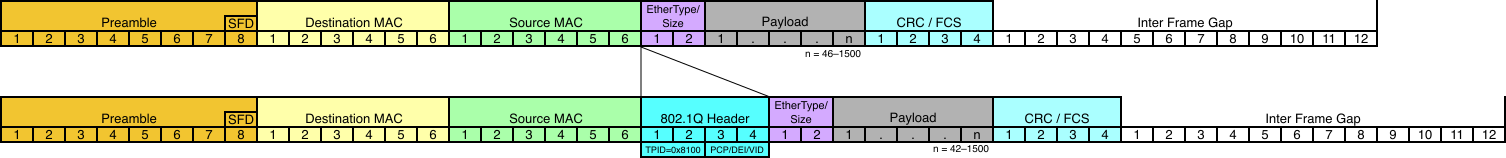
\includegraphics[keepaspectratio,alt={Formato del frame Ethernet con tag 802.1Q VLAN}]{images/Ethernet-802-1Q-Insert-864c1f.png}}
\emph{Fonte: Wikimedia Commons --- Il tag 802.1Q (4 byte, TPID 0x8100)
viene inserito nell'header Ethernet tra Source MAC e EtherType. I 12 bit
del VLAN ID consentono fino a 4094 VLAN distinte.}

Internamente allo switch, ogni pacchetto è \emph{sempre} taggato: se
arriva untagged, il primo passo dell'ASIC è assegnarlo alla VLAN di
default della porta ingress. I pacchetti viaggiano internamente con il
tag, e solo all'uscita su una porta untagged il tag viene rimosso.

\begin{callouttip}{Comportamento del forwarding VLAN}

Un frame entra su porta \texttt{Eth1/1/1} configurata come untagged VLAN
10 → lo switch aggiunge tag VID=10. L'ASIC cerca la MAC destination
nella tabella di forwarding filtrando per VID=10 → trova porta
\texttt{Eth1/1/5} configurata come trunk (tagged). Il frame esce con il
tag 802.1Q intatto. Se la MAC destination fosse invece su una porta
untagged VLAN 10, il frame uscirebbe senza tag.

\end{callouttip}

\subsection{Perché le VLAN sono
Critiche}\label{perchuxe9-le-vlan-sono-critiche}

Le VLAN risolvono due problemi fondamentali del data center:

\textbf{Sicurezza e segregazione}: le VLAN separano il traffico come se
fossero reti fisicamente distinte. Per questo motivo persino le forze
militari --- che tradizionalmente usavano tre reti fisiche separate
(confidenziale, riservato, top secret) --- hanno accettato l'uso di tre
VLAN su una stessa infrastruttura. La garanzia è che un pacchetto in
VLAN A non può mai, per come funziona l'ASIC, raggiungere un host in
VLAN B, a meno di una decisione esplicita di routing.

\textbf{Flessibilità della topologia}: il cablaggio fisico è costoso e
difficile da modificare. Le VLAN permettono di ridisegnare la
segmentazione logica della rete semplicemente riconfigurando il tagging
delle porte, senza toccare un solo cavo. Questo è stato determinante per
rendere i data center agili: si possono creare o eliminare sottoreti in
pochi minuti.

\begin{calloutnote}{VLAN e VRF}

Nelle configurazioni avanzate, le VLAN si associano a \textbf{VRF}
(Virtual Routing and Forwarding) per creare anche tabelle di routing
virtuali distinte. Questo completa la separazione logica all'intero
Layer 3, non solo Layer 2.

\end{calloutnote}

\begin{center}\rule{0.5\linewidth}{0.5pt}\end{center}

\section{Resilienza e Complessità del Debug di
Rete}\label{resilienza-e-complessituxe0-del-debug-di-rete}

La lezione si conclude con una riflessione sul perché la rete sia
progettata così com'è --- funzionale, deterministica, resistente --- e
sul perché il debug di rete sia particolarmente difficile.

Il docente porta due aneddoti dalla propria esperienza diretta con la
rete dell'Università di Pisa:

\begin{enumerate}
\def\labelenumi{\arabic{enumi}.}
\item
  Un \textbf{network loop} (ciclo nella topologia di Layer 2) aveva
  causato un'interruzione. Il loop coinvolgeva migliaia di dispositivi e
  porte, rendendo il processo di individuazione estremamente lungo ---
  al momento della lezione il loop era ancora presente e in fase di
  ricerca.
\item
  Un \textbf{guasto intermittente} su un collegamento in fibra ottica da
  15 km tra due sedi aveva causato un downtime di due-tre giorni. La
  causa era probabilmente un danno fisico alla fibra (una macchina
  agricola aveva transitato sopra il cavo interrato). Il link LACP usava
  due fibre: una funzionante e una degradata. Il risultato era un
  comportamento intermittente difficilissimo da diagnosticare --- metà
  del traffico funzionava, metà generava errori --- con l'apparenza di
  un problema software o di configurazione.
\end{enumerate}

Questi esempi illustrano un principio generale:

\begin{callouttip}{La rete è semplice ma i suoi comportamenti emergenti sono complessi}

Un singolo switch fa una cosa sola: ricevere un pacchetto e decidere su
quale porta inoltrarlo (store-and-forward). L'algoritmo è banale. Ma
quando miliardi di pacchetti al secondo attraversano decine di switch, i
comportamenti emergenti sono di una complessità enorme. Non esiste un
``debugger'' per la rete perché fermare l'esecuzione \emph{cambia} il
comportamento della rete stessa. Per questo tutto in networking --- dal
design del software alla CLI al doppio boot image --- è pensato per
ridurre la probabilità di stati inconsistenti.

\end{callouttip}

\begin{center}\rule{0.5\linewidth}{0.5pt}\end{center}

\section{Conclusioni e Punti Chiave}\label{conclusioni-e-punti-chiave-1}

Questa lezione ha coperto l'intera catena dall'hardware al software
negli switch di rete moderni:

\begin{itemize}
\tightlist
\item
  Lo switch è un \textbf{computer general purpose} con una CPU x86
  (control plane, Linux) e un ASIC specializzato (data plane, silicon
  commodity da Broadcom et al.) collegati via PCIe.
\item
  La distinzione \textbf{control plane / data plane} è il framework
  concettuale fondamentale per capire qualsiasi dispositivo di rete.
\item
  \textbf{SONiC} e \textbf{ONIE} rappresentano la direzione del mercato
  verso la disaggregazione hardware/software, con NOS open source
  intercambiabili come gli OS sui server.
\item
  La \textbf{CLI modale} --- heritage Cisco --- è ancora lo strumento
  primario di configurazione, con il meccanismo running/startup config
  che garantisce il determinismo allo stato di boot.
\item
  Le \textbf{VLAN} (IEEE 802.1Q, 12 bit di VLAN ID, 4094 VLAN possibili)
  sono lo strumento fondamentale per creare broadcast domain virtuali su
  una stessa infrastruttura fisica, abilitando sia la sicurezza che la
  flessibilità topologica.
\item
  Il debug della rete è intrinsecamente difficile a causa del volume di
  traffico e della natura dinamica del sistema: l'approccio funzionale
  (switch che tornano sempre nello stesso stato al riavvio) è la
  risposta architettuale a questo problema.
\end{itemize}

\begin{quote}
\begin{itemize}
\tightlist
\item
  Spiega il naming \texttt{1/1/3} di una porta su uno switch stack.
\end{itemize}
\end{quote}

\newpage

\chapter{Lezione 8 --- Switch e Fabric
continua}\label{lezione-8-switch-e-fabric-continua}

\section{Ethernet come standard de
facto}\label{ethernet-come-standard-de-facto}

Il punto di partenza è riconoscere il ruolo attuale dello switch di
rete: non è più semplicemente un modo per connettere computer a
Internet, ma è il meccanismo con cui si aggregano elementi
computazionali in blocchi più grandi. In questo contesto, il traffico
dominante nei data center è il cosiddetto \textbf{east-west traffic} ---
cioè il traffico tra server all'interno dello stesso data center ---
anziché il tradizionale traffico north-south verso l'esterno.

Ethernet è diventato lo standard di connessione locale non perché fosse
tecnicamente il migliore, ma perché era il più adottato. La diffusione
di massa ha generato economie di scala che hanno abbassato i costi
dell'hardware e stimolato lo sviluppo di un ecosistema software
enormemente ricco. Originariamente Ethernet era progettato per un
singolo cavo coassiale condiviso --- un bus fisico --- ma questa
architettura fisica non esiste più: oggi si emula virtualmente, e tutta
l'infrastruttura software costruita su di essa è il vero motivo per cui
continuiamo a usarla.

\begin{callouttip}{Intuizione chiave}

Ethernet non ha vinto per meriti tecnici assoluti, ma per effetto di
rete: più utenti → più volumi → costi più bassi → ancora più utenti.
Questa dinamica si ripete in molte tecnologie informatiche.

\end{callouttip}

Quando i requisiti cambiano, lo standard viene esteso anziché
rimpiazzato. Le VLAN ne sono l'esempio più importante: aggiungono un tag
all'header Ethernet per consentire la segmentazione logica della rete.

\begin{center}\rule{0.5\linewidth}{0.5pt}\end{center}

\section{MTU e dimensione dei
pacchetti}\label{mtu-e-dimensione-dei-pacchetti}

\begin{calloutdefinition}{MTU — Maximum Transmission Unit}

La dimensione massima di un frame (pacchetto) che un dispositivo di rete
è configurato ad accettare. Il valore di default in Ethernet è
\textbf{1,5 KB} (più precisamente 1500 byte).

\end{calloutdefinition}

Sapere quanto è grande un pacchetto di rete è fondamentale per capire le
prestazioni. Ogni unità di elaborazione di rete implementa un loop del
tipo \emph{``per ogni pacchetto, fai qualcosa''}: se i pacchetti sono
molti e piccoli, il numero di iterazioni cresce, aumentando il carico
sulla CPU. Se i pacchetti sono grandi, diminuisce il numero di
iterazioni ma si richiede più memoria per i buffer.

Questo compromesso ha una conseguenza pratica: \textbf{i frame Jumbo}.
Nei data center è possibile configurare switch per accettare frame da
\textbf{9 KB} (fattore 6 rispetto al default). Questo è stato introdotto
quando si iniziò a usare Ethernet per il traffico di storage, dove
trasferire molti dati con un overhead basso è critico.

\begin{calloutwarning}{Attenzione: consistenza dell’MTU nella rete}

In una rete a più switch (es. topologia a tre livelli), tutti i
dispositivi lungo un percorso devono avere lo stesso MTU configurato. Se
un frame da 9 KB arriva su un link con MTU 1,5 KB, il ricevente deve
frammentarlo in 6 pacchetti più piccoli --- vanificando il vantaggio del
jumbo frame e aggiungendo lavoro inutile. L'MTU è uno dei parametri di
configurazione più sottovalutati e fonte di problemi difficili da
diagnosticare.

\end{calloutwarning}

\begin{center}\rule{0.5\linewidth}{0.5pt}\end{center}

\section{Control plane, CLI e filosofia delle command
line}\label{control-plane-cli-e-filosofia-delle-command-line}

I parametri come l'MTU si configurano attraverso il \textbf{control
plane} dello switch, tipicamente tramite una \textbf{CLI} (Command Line
Interface). La CLI degli switch di rete ha una struttura modale: si
entra in un contesto (es. \texttt{vlan\ 3}), si emettono comandi
specifici, poi si esce. Questa filosofia si è diffusa ben oltre il
networking: il comando \texttt{ip} di Linux, \texttt{netsh} di Windows,
e persino \texttt{docker} e altri strumenti moderni adottano lo stesso
paradigma di \emph{verbo + sottocomando}.

\begin{calloutnote}{Nota filosofica: Unix vs CLI moderna}

La filosofia Unix tradizionale prevedeva comandi piccoli e atomici
(\texttt{cp}, \texttt{ls}, \texttt{sort}) composti tramite pipe per
costruire comportamenti complessi. La filosofia moderna, nata
probabilmente con Docker, preferisce un singolo comando ``grasso'' con
molti sottocomandi (\texttt{docker\ ps}, \texttt{docker\ image},
\texttt{docker\ exec}). Questo riduce la componibilità ma semplifica la
gestione e il versionamento quando il numero di risorse da gestire è
molto elevato.

\end{calloutnote}

\begin{center}\rule{0.5\linewidth}{0.5pt}\end{center}

\section{VLAN: segmentazione logica del broadcast
domain}\label{vlan-segmentazione-logica-del-broadcast-domain}

\begin{calloutdefinition}{VLAN — Virtual LAN}

Una VLAN è un tag inserito nell'header Ethernet che identifica il
\textbf{broadcast domain} di appartenenza di un frame. Permette di
dividere logicamente una rete fisica in più reti separate, senza
modificare il cablaggio.

\end{calloutdefinition}

Il meccanismo è semplice: quando un frame non taggato arriva su una
porta configurata come \emph{untagged} di una certa VLAN, lo switch lo
riscrive aggiungendo il VLAN ID corrispondente. Tutti i frame
all'interno dello switch vengono quindi trattati con il loro VLAN ID,
garantendo isolamento tra broadcast domain diversi.

\subsection{Porte access e trunk}\label{porte-access-e-trunk}

Quando una porta è associata a un unico VLAN ID con traffico non
taggato, si parla di porta in \textbf{modalità access}: tipicamente
usata per connettere un singolo host che non deve preoccuparsi del
tagging. Quando invece una porta è associata a più VLAN ID (con traffico
taggato), si parla di porta in \textbf{modalità trunk}: è usata per i
collegamenti tra switch, dove è necessario trasportare il traffico di
più broadcast domain sullo stesso cavo fisico.

\begin{callouttip}{Esempio pratico}

Un data center ha due rack connessi da un singolo cavo tra i rispettivi
leaf switch. Quel cavo deve trasportare il traffico di VLAN 2 e VLAN 3
simultaneamente. La porta su entrambi gli switch viene configurata come
trunk con VLAN 2 e 3 tagged. In questo modo non è necessario un cavo per
ogni VLAN.

\end{callouttip}

\subsection{VLAN nella topologia
spine-leaf}\label{vlan-nella-topologia-spine-leaf}

In un'architettura spine-leaf, le porte sui leaf switch che si collegano
verso la spine vengono configurate con tutti i VLAN ID in uso. Ogni
frame che arriva su un leaf taggato con un certo VLAN ID viene inoltrato
verso la spine solo se la porta di uplink include quel VLAN ID nel
trunk. Questo permette di avere una rete logicamente ricca su una
topologia fisica molto regolare.

\begin{calloutwarning}{Limite fondamentale delle VLAN}

Lo standard 802.1Q supporta al massimo \textbf{4096 VLAN ID} (12 bit).
Per una cloud pubblica con milioni di tenant, questo numero è
assolutamente insufficiente.

\end{calloutwarning}

\begin{center}\rule{0.5\linewidth}{0.5pt}\end{center}

\section{VXLAN e overlay network}\label{vxlan-e-overlay-network}

Il limite delle 4096 VLAN, combinato con la difficoltà di gestire
manualmente la configurazione di ogni switch, ha portato allo sviluppo
del \textbf{VXLAN} (\emph{Virtual Extensible LAN}).

\begin{calloutdefinition}{VXLAN}

VXLAN è un protocollo di \textbf{overlay network}: incapsula il traffico
di layer 2 (Ethernet) all'interno di pacchetti UDP di layer 3 (IP).
Questo permette di simulare reti layer 2 arbitrarie su un'infrastruttura
layer 3 esistente.

\end{calloutdefinition}

\subsection{Perché conviene lavorare a layer
3}\label{perchuxe9-conviene-lavorare-a-layer-3}

Operare a livello IP (layer 3) offre vantaggi critici rispetto al layer
2 puro:

\begin{itemize}
\tightlist
\item
  \textbf{Debug molto più semplice}: a layer 3 ogni pacchetto ha
  sorgente e destinazione ben definite; è possibile tracciare il
  percorso e isolare i problemi. A layer 2, un loop di broadcast può
  abbattere interi domini broadcast senza che sia facile capire dove si
  trova il problema.
\item
  \textbf{Scalabilità}: i VXLAN network identifier sono a 24 bit, ovvero
  circa \textbf{16 milioni} di segmenti virtuali --- ordini di grandezza
  superiori alle 4096 VLAN.
\item
  \textbf{Automazione}: i segmenti virtuali vengono creati e gestiti via
  software, senza intervento manuale su ogni switch fisico.
\end{itemize}

\begin{callouttip}{Esempio reale: università di Pisa}

Il core network dell'università usa VXLAN per collegare i diversi
dipartimenti. Quando c'è stato un incidente alla facoltà di ingegneria,
fu necessario ripristinare rapidamente la connettività creando link
layer 2 temporanei. Questo introdusse un loop che causò l'interruzione
del servizio. La lezione appresa: reti layer 2 estese sono difficili da
debuggare; lavorare a layer 3 con VXLAN riduce drasticamente questo
rischio.

\end{callouttip}

\subsection{Architettura VXLAN in
produzione}\label{architettura-vxlan-in-produzione}

In Azure (e provider simili), ogni rack del data center è un dominio
layer 2. Tutto il traffico che esce dal rack viene immediatamente
incapsulato in layer 3. Questo rende il troubleshooting molto più
efficace: ogni flusso ha un identificatore IP univoco e può essere
tracciato indipendentemente.

\begin{calloutnote}{Sintesi VLAN vs VXLAN}

Le VLAN segmentano un dominio broadcast fisico usando tag nell'header
Ethernet (layer 2). VXLAN crea reti layer 2 virtuali incapsulando il
traffico in UDP/IP (layer 3). VXLAN richiede un control plane: questo è
svolto da \textbf{EVPN} (\emph{Ethernet VPN}), il protocollo che
gestisce la distribuzione delle informazioni di raggiungibilità tra i
nodi VXLAN.

\end{calloutnote}

\begin{center}\rule{0.5\linewidth}{0.5pt}\end{center}

\section{Protocolli implementati da uno
switch}\label{protocolli-implementati-da-uno-switch}

Uno switch moderno è molto più di un semplice dispositivo di forwarding.
Implementa decine di protocolli, tra cui:

\textbf{Switching e VLAN:} IEEE 802.1Q (VLAN tagging), 802.1ad (Q-in-Q,
per incapsulare VLAN dentro altre VLAN), Spanning Tree Protocol e
varianti (per prevenire loop).

\textbf{Quality of Service:} ETS (\emph{Enhanced Transmission
Selection}) per il controllo di flusso, PFC (\emph{Priority Flow
Control}) per la prioritizzazione del traffico. Questi standard, nati
per il traffico storage (dove i dischi non possono aspettare),
permettono di suddividere la banda tra fino a 16 classi di traffico con
diverse priorità.

\begin{calloutnote}{Il mito di Ethernet senza QoS}

Si sente spesso dire che Ethernet non supporta Quality of Service. Non è
vero: il puro standard IEEE 802.3 non ha flow control, ma le estensioni
ETS e PFC, presenti in tutti gli switch data center moderni, forniscono
proprio questo. Quello che è ``lento'' non è Ethernet, ma TCP.

\end{calloutnote}

\textbf{Overlay e virtualizzazione:} VXLAN, EVPN, MAC-in-UDP per il
tunneling layer 2 su layer 3.

\textbf{Routing:} OSPF, BGP, ARP, protocolli multicast.

\textbf{Gestione:} SNMP per il monitoring, syslog, NetFlow per l'analisi
del traffico, LLDP/CDP per la discovery della topologia.

\begin{center}\rule{0.5\linewidth}{0.5pt}\end{center}

\section{OpenFlow e Software Defined
Networking}\label{openflow-e-software-defined-networking}

\subsection{Il problema della ricerca in
rete}\label{il-problema-della-ricerca-in-rete}

Intorno al 2008, ricercatori di Stanford identificarono un problema: i
network administrator non permettevano di sperimentare su switch reali
perché troppo critici. La ricerca in networking era bloccata.

\subsection{La flow table}\label{la-flow-table}

Per capire OpenFlow occorre capire come funziona internamente uno
switch: i dispositivi moderni mantengono una \textbf{flow table}, una
struttura dati che associa pattern di traffico ad azioni. Anziché
rieseguire ogni volta tutta la logica di configurazione per ogni
pacchetto, lo switch costruisce regole del tipo:

\begin{quote}
Se (source MAC = X) AND (destination IP = Y) AND (VLAN = Z) → output
porta 2
\end{quote}

Una volta che un flusso è noto, questa regola viene eseguita
direttamente in hardware, senza ricalcolare tutto da capo. La flow table
include anche contatori, utili per il debugging e il monitoring.

\begin{calloutdefinition}{OpenFlow}

OpenFlow è un'\textbf{API standard} che permette a un controller esterno
di leggere e modificare la flow table di uno switch. Il controller ---
un processo software su un server normale --- può aggiungere, modificare
o rimuovere regole in risposta a eventi di rete.

\end{calloutdefinition}

\subsection{Applicazioni pratiche}\label{applicazioni-pratiche}

\textbf{Firewall sandwich:} si inserisce un firewall L7 tra due switch.
Il primo switch reindirizza ogni nuovo flusso attraverso il firewall;
quando il firewall approva il flusso, il controller OpenFlow aggiorna la
flow table dello switch per far bypassare il firewall ai pacchetti
successivi dello stesso flusso. Risultato: si ispeziona solo l'inizio
del flusso, il resto transita alla massima velocità.

\textbf{Mirroring e honeypot:} OpenFlow permette di copiare
selettivamente il traffico su una porta di monitoraggio (per un sistema
IDS) o di redirigere traffico sospetto verso un honeypot --- un sistema
esca che simula un target reale per catturare e studiare gli attaccanti.

\begin{calloutnote}{Stato attuale di OpenFlow}

Nato con grandi ambizioni di ``open networking'', 15 anni dopo OpenFlow
è principalmente uno strumento di ricerca e viene usato in casi
specifici. La maggior parte dei professionisti non lo usa mai. È
comunque importante conoscerne l'esistenza e il principio.

\end{calloutnote}

\begin{center}\rule{0.5\linewidth}{0.5pt}\end{center}

\section{Latenza in Ethernet}\label{latenza-in-ethernet}

Bandwidth e latenza sono i due parametri fondamentali che governano le
prestazioni di rete. La latenza si misura in diversi modi:

\begin{itemize}
\tightlist
\item
  \textbf{Serialization latency}: tempo per mettere i bit sul cavo. Con
  1 Gigabit era \textasciitilde12 µs; con le tecnologie moderne siamo
  nell'ordine di \textbf{300 ns}.
\item
  \textbf{Propagation latency}: tempo di propagazione del segnale sul
  cavo. A 10 metri siamo \textasciitilde50 ns, trascurabile nella
  maggior parte dei casi.
\item
  \textbf{Switch latency} (cut-through): tempo di attraversamento di uno
  switch. I chipset Broadcom Trident/Tomahawk sono tipicamente tra
  \textbf{400 e 700 ns}.
\item
  \textbf{End-to-end con TCP}: il protocollo TCP aggiunge overhead di
  framing, finestre di congestione, ACK, ecc. La latenza tipica di uno
  stream TCP è di circa \textbf{70 µs} --- ordini di grandezza superiore
  al solo hardware.
\end{itemize}

\begin{callouttip}{Intuizione chiave}

Ethernet in sé è \textbf{low latency}. TCP non lo è. Quando si sente
dire che ``Ethernet non è adatto all'HPC perché ha troppa latenza'', il
problema è quasi sempre il protocollo TCP sopra, non il mezzo fisico.

\end{callouttip}

\begin{center}\rule{0.5\linewidth}{0.5pt}\end{center}

\section{InfiniBand e RDMA:
introduzione}\label{infiniband-e-rdma-introduzione}

\subsection{Perché InfiniBand}\label{perchuxe9-infiniband}

Quando il 1 Gigabit Ethernet aveva latenza di 12 µs, era chiaramente
inadeguato per applicazioni HPC (High Performance Computing) dove il
pattern computazionale è \emph{calcola → comunica → calcola → comunica}
in cicli molto stretti. InfiniBand è nato per rispondere a questa
esigenza.

\begin{calloutdefinition}{InfiniBand}

InfiniBand è uno standard di interconnessione progettato per HPC, con
latency di \textbf{1-2 µs} end-to-end (confrontare con i 70 µs di TCP su
Ethernet). La MTU di un pacchetto InfiniBand è di \textbf{2 GB} ---
enormemente più grande rispetto ai 9 KB dei jumbo frame Ethernet. Molte
funzioni che in Ethernet sono software sono implementate direttamente in
silicio.

\end{calloutdefinition}

InfiniBand è stato a lungo dominato da \textbf{Mellanox}, un'azienda
israeliana acquisita da \textbf{Nvidia} nel 2020. Nvidia ora usa questa
tecnologia per la connessione ad alta velocità tra GPU nei cluster di
training AI (fabric NVLink/NVSwitch).

\subsection{RDMA e RoCE}\label{rdma-e-roce}

\begin{calloutdefinition}{RDMA — Remote Direct Memory Access}

RDMA permette a un host di rete di scrivere direttamente nella memoria
di un altro host \textbf{senza coinvolgere la CPU del destinatario}.
Analogo alla DMA locale (il meccanismo con cui un disco scrive in RAM
senza impegnare la CPU), ma attraverso la rete.

\end{calloutdefinition}

Questo elimina drasticamente la latenza software: non c'è interrupt, non
c'è context switch, non c'è copia di dati. La latenza risultante è
paragonabile a quella dell'hardware di rete.

Poiché InfiniBand era costoso e richiedeva hardware dedicato, Mellanox
ha proposto \textbf{RoCE} (\emph{RDMA over Converged Ethernet}):

\begin{calloutdefinition}{RoCE — RDMA over Converged Ethernet}

RoCE implementa RDMA su Ethernet, sfruttando le estensioni di QoS (ETS e
PFC) per garantire l'affidabilità necessaria. È supportato nativamente
su Linux e Windows, ed è oggi lo standard per HPC su Ethernet.

\end{calloutdefinition}

\begin{calloutnote}{Dove siamo oggi}

InfiniBand rimane in uso nei cluster HPC tradizionali per la latenza e
per la sua topologia ottimizzata (fat tree senza oversubscription).
RoCE/RDMA ha eroso parte del suo vantaggio portando latenze simili su
Ethernet. Nella prossima lezione si esaminerà più in dettaglio la
topologia \textbf{fat tree} (\emph{full fat tree}) usata in InfiniBand,
che garantisce banda costante indipendentemente dal numero di hop nella
rete.

\end{calloutnote}

\begin{center}\rule{0.5\linewidth}{0.5pt}\end{center}

\section{Roadmap delle prossime
lezioni}\label{roadmap-delle-prossime-lezioni}

Dopo InfiniBand e le topologie HPC, il corso proseguirà con:

\begin{itemize}
\tightlist
\item
  Storage, drive e ridondanza (RAID e storage distribuito)
\item
  Risalita sullo stack verso virtualizzazione e hypervisor
\item
  Sicurezza di rete e firewall L7
\end{itemize}

\begin{quote}
\begin{itemize}
\tightlist
\item
  Cos'è RoCE e in quale contesto è stato introdotto?
\end{itemize}
\end{quote}

\newpage

\chapter{Fabric Avanzato e Introduzione allo
Storage}\label{fabric-avanzato-e-introduzione-allo-storage}

\section{Workload e architettura del
datacenter}\label{workload-e-architettura-del-datacenter}

Prima di parlare di fabric ad alte prestazioni, è necessario capire
\emph{perché} esistono. La scelta dell'architettura di rete di un
datacenter --- larghezza di banda, latenza, topologia --- non è
universale: è guidata dal tipo di workload che il sistema deve eseguire.
Il professore distingue quattro categorie fondamentali.

\textbf{HPC} (\emph{High Performance Computing}) è la categoria più
antica: si tratta di problemi computazionalmente enormi --- simulazioni
fisiche, fluidodinamica, modellazione sismica --- che un singolo
computer non può risolvere in tempo utile. La soluzione è decomporre il
problema in sotto-problemi assegnati a nodi omogenei (tutti con le
stesse risorse), che collaborano comunicando frequentemente. Il classico
esempio è ENI che simula la propagazione delle onde sismiche nel
sottosuolo tramite elementi finiti per individuare giacimenti
petroliferi senza trivellare: il risultato arriva in sei mesi usando
migliaia di CPU, mentre con un singolo computer richiederebbe secoli.

\textbf{Cloud} è il modello inverso: qui il problema è piccolo --- una
singola applicazione web, un microservizio --- e il server è talmente
potente da poter ospitare decine o centinaia di macchine virtuali
contemporaneamente. La relazione è uno-a-molti: un computer, molti
problemi. Questo modello è stato possibile perché per vent'anni la
potenza computazionale è cresciuta molto più velocemente della domanda
software.

\textbf{Big Data} è orientato all'elaborazione di quantità enormi di
dati, tipicamente con dischi meccanici: la latenza d'accesso allo
storage (millisecondi) è così dominante che la latenza di rete diventa
irrilevante. Non ha senso ottimizzare la rete se il collo di bottiglia è
il disco.

\textbf{AI/ML} è la categoria che ha recentemente rotto l'equilibrio del
cloud: si tratta di workload che, come l'HPC, richiedono uno o più
server dedicati per un singolo calcolo. Il professore distingue due
sotto-categorie con requisiti molto diversi --- \textbf{training} e
\textbf{inference} --- e sottolinea che anche i laptop moderni montano
oggi un NPU (\emph{Neural Processing Unit}) ottimizzato per l'inferenza
locale.

\begin{callouttip}{Intuizione chiave}

La latenza di rete conta solo quando la computazione è
\emph{memory-bound} e \emph{sincronizzata}. In HPC e AI training ogni
nodo deve aspettare gli altri a ogni passo: anche 2 ms di latenza di
rete moltiplicati per milioni di iterazioni diventano il collo di
bottiglia. In Big Data il disco è così lento (ms) che la rete smette di
importare.

\end{callouttip}

\begin{center}\rule{0.5\linewidth}{0.5pt}\end{center}

\section{InfiniBand}\label{infiniband}

\subsection{Contesto storico e
motivazione}\label{contesto-storico-e-motivazione}

Quando InfiniBand fu introdotto, Ethernet era ancora a 1 Gigabit per
secondo. Per aggregare 5 Gbps su un server si usavano 4-5 cavi Ethernet.
InfiniBand offriva in un singolo cavo \textasciitilde80 Gbps --- da qui
il nome, che richiamava la \emph{larghezza di banda infinita}. Oggi il
confronto con Ethernet è molto meno netto dal punto di vista della
banda, ma InfiniBand mantiene un vantaggio significativo in
\textbf{latenza}.

\begin{calloutdefinition}{InfiniBand}

Fabric di rete ad alte prestazioni progettata per ambienti HPC.
Fisicamente simile a Ethernet (connettori SFP/QSFP), radicalmente
diversa a livello di protocollo. Originariamente sviluppata da Mellanox,
oggi di proprietà NVIDIA.

\end{calloutdefinition}

\subsection{Caratteristiche del
protocollo}\label{caratteristiche-del-protocollo}

La differenza cruciale rispetto a Ethernet non è nei cavi, ma nel
protocollo:

\begin{itemize}
\tightlist
\item
  \textbf{Pacchetti fino a 2 GB}: dal punto di vista del software host,
  si può inviare un pacchetto da 2 gigabyte come unità atomica. Il
  fabric si occupa internamente della segmentazione e riassemblaggio, ma
  l'applicazione non deve preoccuparsene.
\item
  \textbf{16 classi di priorità} (\emph{QoS} nativo): è possibile
  classificare il traffico con granularità fine.
\item
  \textbf{IP over IB}: esiste un adattatore per far girare TCP/IP sopra
  InfiniBand, utile per la comunicazione \emph{north-south} verso
  l'esterno, ma nessuno lo usa per comunicazioni interne al cluster.
\end{itemize}

La topologia tipica di un cluster InfiniBand è: \textbf{east-west su
InfiniBand} (comunicazione tra nodi del cluster), \textbf{north-south su
Ethernet} (comunicazione con l'esterno). Il nodo di testa del cluster
(\emph{head node}) è l'unico connesso a entrambe le reti.

Uno switch InfiniBand può arrivare a 128 porte in un singolo chassis:
questo permette di implementare in hardware un'interconnessione
completamente piatta con latenza garantita sotto i 3 microsecondi tra
qualsiasi coppia di porte.

\subsection{Top500: lo stato dell'arte}\label{top500-lo-stato-dellarte}

Il \emph{Top500} è la classifica dei 500 supercomputer più potenti al
mondo. Tutti i sistemi nelle prime posizioni usano InfiniBand o
Slingshot. Il professore cita come esempi:

{\def\LTcaptype{none} % do not increment counter
\begin{longtable}[]{@{}
  >{\raggedright\arraybackslash}p{(\linewidth - 4\tabcolsep) * \real{0.3750}}
  >{\raggedright\arraybackslash}p{(\linewidth - 4\tabcolsep) * \real{0.3750}}
  >{\raggedright\arraybackslash}p{(\linewidth - 4\tabcolsep) * \real{0.2500}}@{}}
\toprule\noalign{}
\begin{minipage}[b]{\linewidth}\raggedright
Sistema
\end{minipage} & \begin{minipage}[b]{\linewidth}\raggedright
Potenza
\end{minipage} & \begin{minipage}[b]{\linewidth}\raggedright
Note
\end{minipage} \\
\midrule\noalign{}
\endhead
\bottomrule\noalign{}
\endlastfoot
Frontier & \textasciitilde29 MW, \textasciitilde11M core & AMD + GPU
Instinct, Slingshot (HPE) \\
Eagle & --- & Microsoft Azure, NVIDIA H100, InfiniBand --- architettura
di riferimento per AI \\
Leonardo & --- & Italia, top 10 \\
Jupiter & --- & Germania, primo sistema europeo exascale \\
\end{longtable}
}

\textbf{Slingshot} (HPE/Cray) è Ethernet ``su steroidi'': compatibile
Ethernet a livello fisico, ma con ottimizzazioni di protocollo per bassa
latenza. \textbf{InfiniBand} (NVIDIA) è il protocollo nativo per HPC. I
due dominano il segmento dei supercomputer.

\begin{center}\rule{0.5\linewidth}{0.5pt}\end{center}

\section{MPI e RDMA}\label{mpi-e-rdma}

\subsection{MPI: Message Passing
Interface}\label{mpi-message-passing-interface}

Prima di parlare di RDMA, è fondamentale capire il contesto del software
HPC. Quasi tutto il codice HPC distribuito è scritto usando \textbf{MPI}
(\emph{Message Passing Interface}), una libreria C di \textasciitilde35
anni che esprime la computazione distribuita come scambio di messaggi
tra nodi identificati da un numero progressivo (non da indirizzi di
rete).

\begin{callouttip}{Intuizione chiave}

MPI astrae completamente il fabric sottostante. L'applicazione invia
``un messaggio al nodo 4'' e MPI si occupa di tradurre questo in
chiamate alle primitive di rete specifiche del fabric disponibile ---
InfiniBand, Slingshot, Ethernet. Questo è il motivo per cui la community
HPC ha potuto cambiare fabric multiple volte senza riscrivere il codice
applicativo.

\end{callouttip}

\subsection{RDMA: Remote Direct Memory
Access}\label{rdma-remote-direct-memory-access}

\textbf{RDMA} estende il concetto di DMA (\emph{Direct Memory Access})
--- il meccanismo che permette a una periferica di leggere/scrivere
direttamente in RAM senza coinvolgere la CPU --- attraverso la rete.

Il meccanismo sfrutta le schede di rete \emph{converged NIC}, collegate
al bus PCIe: queste schede possono leggere e scrivere nella RAM del
server remoto direttamente, senza passare per il sistema operativo del
destinatario.

\begin{calloutwarning}{Implicazioni di sicurezza}

RDMA bypassa il sistema operativo: la scheda di rete ha accesso diretto
alla memoria. Questo introduce rischi di sicurezza non banali che vanno
considerati nel design del sistema.

\end{calloutwarning}

RDMA è diventato lo standard \emph{de facto} per la comunicazione a
bassa latenza in ambienti distribuiti. Dal 2016, anche Windows
implementa \textbf{RoCE} (\emph{RDMA over Converged Ethernet}), portando
RDMA anche su Ethernet standard.

\subsection{Confronto di latenza}\label{confronto-di-latenza}

{\def\LTcaptype{none} % do not increment counter
\begin{longtable}[]{@{}ll@{}}
\toprule\noalign{}
Tecnologia & Latenza tipica \\
\midrule\noalign{}
\endhead
\bottomrule\noalign{}
\endlastfoot
InfiniBand nativo (RDMA) & 1--3 μs \\
RoCE (RDMA over Converged Ethernet) & 1.3--5 μs \\
IP over InfiniBand & 5--15 μs \\
TCP/IP su Ethernet & 20--70+ μs \\
\end{longtable}
}

Il dato più significativo: aggiungere il protocollo IP sopra InfiniBand
\textbf{moltiplica per 4-5x la latenza} rispetto a RDMA nativo. TCP/IP è
ulteriormente peggiore. Questo spiega perché per HPC nessuno usa TCP/IP
interno al cluster.

\begin{calloutnote}{L’inventore di TCP/IP e i buffer}

Il professore cita un aneddoto: uno degli autori di TCP/IP, analizzando
la lentezza della propria rete domestica, scoprì che il problema era il
buffering introdotto in ogni switch e router. TCP/IP era stato
progettato per essere \emph{adattivo} e senza buffer: l'accumulo di
buffer nella rete moderna ne snatura il comportamento. L'autore commentò
che, se dovesse progettare il protocollo oggi, lo farebbe diversamente.

\end{calloutnote}

\begin{center}\rule{0.5\linewidth}{0.5pt}\end{center}

\section{Overbooking e topologia Full Fat
Tree}\label{overbooking-e-topologia-full-fat-tree}

\subsection{Overbooking}\label{overbooking}

In qualsiasi rete commutata esiste il concetto di \textbf{overbooking}:
il traffico aggregato generabile dai nodi di accesso supera la capacità
del collegamento verso lo strato superiore.

\begin{callouttip}{Esempio concreto}

Uno switch con 48 porte da 25 Gbps e 6 porte uplink da 100 Gbps.
Traffico massimo east-west: 48 × 25 = 1.200 Gbps. Uplink totale: 6 × 100
= 600 Gbps. Il rapporto di overbooking è \textbf{2:1}: i nodi possono
generare il doppio di quanto il fabric possa trasmettere verso lo spine.
Questo è normale e atteso --- la rete si adatta.

\end{callouttip}

\subsection{Full Fat Tree}\label{full-fat-tree}

Per applicazioni HPC dove la latenza e il throughput non-bloccante sono
requisiti, esiste una topologia specifica: il \textbf{Full Fat Tree}.

\begin{calloutdefinition}{Full Fat Tree}

Topologia di rete ad albero in cui la banda dell'uplink di ogni nodo è
uguale alla \emph{somma} delle bande dei link del sottoalbero che
connette. Il risultato è una rete \textbf{non-bloccante}: ogni nodo può
trasmettere a piena velocità verso qualsiasi altro nodo senza contesa.

\end{calloutdefinition}

\pandocbounded{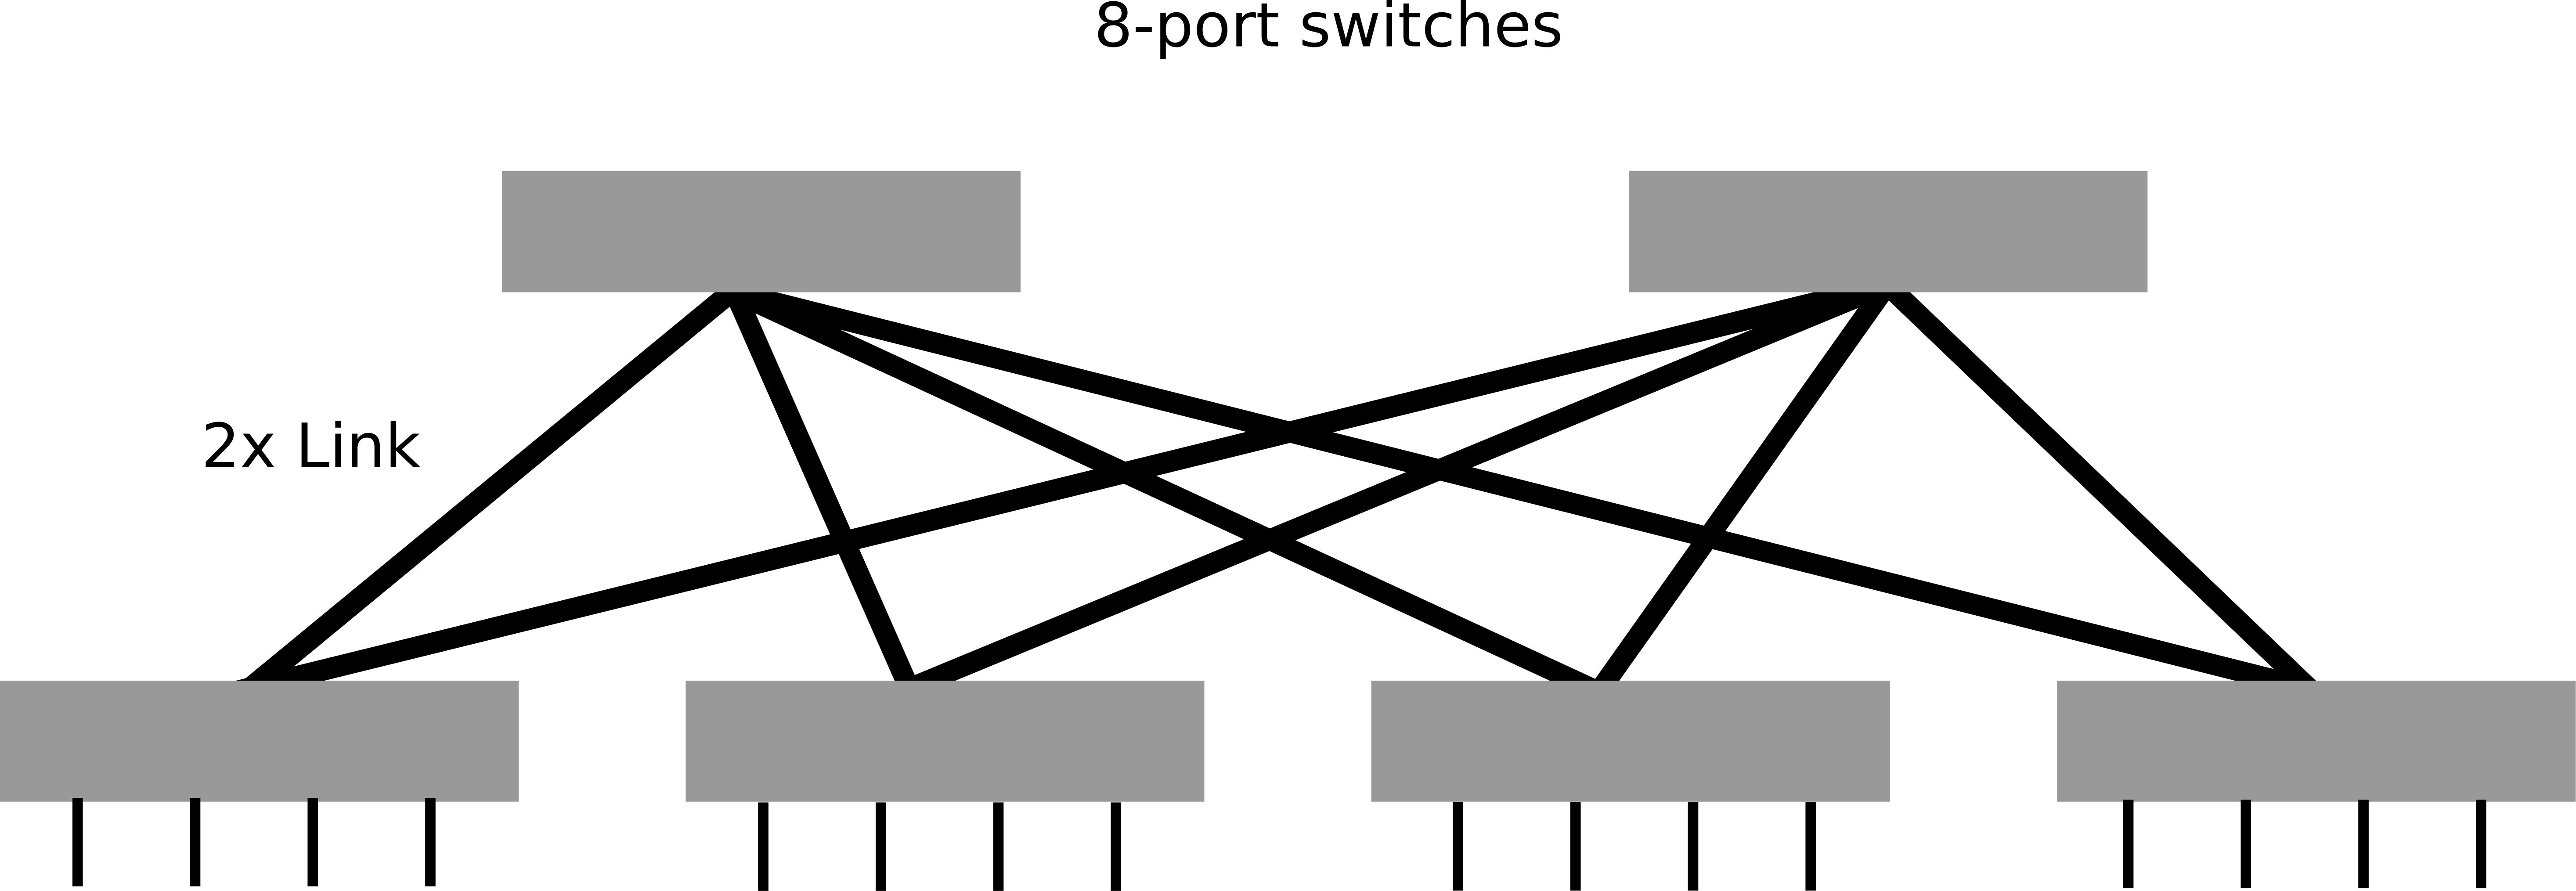
\includegraphics[keepaspectratio,alt={Topologia Full Fat Tree: albero non-bloccante con uplink uguale alla somma dei downlink}]{images/Fat-tree-92c71e.png}}
\emph{Fonte: Wikimedia Commons --- Topologia Fat Tree: ogni nodo
intermedio ha una banda uplink pari alla somma delle bande dei link
verso le foglie. Nessun punto di strozzatura nella rete.}

In pratica, con link aggregation moderna, si implementa sommando più
cavi standard in un link logico. La regola è semplice: se voglio che
metà delle porte serva i server (east-west) e metà vada verso lo spine
(north-south), la banda dei due lati è identica --- nessun overbooking.

Il Full Fat Tree ha un costo elevato (gli switch agli strati superiori
devono gestire bande crescenti), ma è la topologia usata per
supercomputer e cluster HPC dove il throughput non-bloccante è non
negoziabile.

\begin{calloutnote}{Fat Tree vs Spine-and-Leaf}

L'architettura Spine-and-Leaf vista nelle lezioni precedenti
\emph{ricorda} il Fat Tree, ma tipicamente introduce overbooking. Il Fat
Tree è la versione non-bloccante dello Spine-and-Leaf, applicata quando
il costo è giustificato dalle prestazioni richieste.

\end{calloutnote}

\begin{center}\rule{0.5\linewidth}{0.5pt}\end{center}

\section{Fibre Channel: il fabric per lo
storage}\label{fibre-channel-il-fabric-per-lo-storage}

Oltre a Ethernet e InfiniBand, nei datacenter esiste un terzo tipo di
fabric dedicato allo storage: il \textbf{Fibre Channel}.

\begin{calloutdefinition}{Fibre Channel}

Fabric di rete ottico dedicato alla connessione host-storage.
Fisicamente simile a Ethernet e InfiniBand (fibra ottica, connettori
analoghi), ma con protocolli completamente diversi orientati all'accesso
allo storage.

\end{calloutdefinition}

L'architettura tipica è: server con scheda \textbf{HBA}
(\emph{Host-Based Adapter}, l'equivalente Fibre Channel della NIC) →
fabric Fibre Channel (switch FC) → storage array (un sistema con molti
dischi interni). L'HBA emula un disco locale, ma i dati risiedono sullo
storage array.

Il protocollo trasportato da Fibre Channel è \textbf{SCSI} (o più
precisamente FCP --- Fibre Channel Protocol che incapsula SCSI), che
porta a una curiosità storica importante.

Esiste anche \textbf{FCoE} (\emph{Fibre Channel over Ethernet}), pensato
come meccanismo di transizione per evitare di mantenere una rete FC
separata. Il professore lo definisce ``terrible'' --- non funziona bene
ed è stato sostanzialmente abbandonato.

Il Fibre Channel è oggi \textbf{legacy}: molte installazioni esistenti
lo usano ancora, ma i nuovi progetti preferiscono Ethernet o InfiniBand
anche per lo storage.

\begin{center}\rule{0.5\linewidth}{0.5pt}\end{center}

\section{La storia dei protocolli di
storage}\label{la-storia-dei-protocolli-di-storage}

Per capire perché Fibre Channel usa ancora SCSI, occorre ripercorrere la
storia dei protocolli di accesso ai dischi.

\subsection{SCSI: 1979}\label{scsi-1979}

\textbf{SCSI} (\emph{Small Computer System Interface}) nasce nel 1979
come bus parallelo (cavo flat multi-connettore) per collegare più
dispositivi di storage a un singolo controller, condividendo il costo
del controller tra più dischi. La logica master/slave permetteva di
gestire 2 dischi per controller (ATA) o molti di più (SCSI).

Sebbene la tecnologia fisica sia cambiata radicalmente, il
\textbf{protocollo SCSI è sopravvissuto per 40 anni} grazie al principio
di non dover riscrivere il software: ogni nuova tecnologia ha
implementato SCSI come adattatore sopra nuovi mezzi fisici.

{\def\LTcaptype{none} % do not increment counter
\begin{longtable}[]{@{}lll@{}}
\toprule\noalign{}
Variante & Mezzo fisico & Note \\
\midrule\noalign{}
\endhead
\bottomrule\noalign{}
\endlastfoot
SCSI parallelo & Cavo flat & Originale 1979 \\
SAS & Seriale & Serial Attached SCSI \\
iSCSI & Ethernet/TCP & SCSI sopra Internet --- alto overhead \\
FCP & Fibre Channel & SCSI sopra fibra ottica \\
SRP & InfiniBand & SCSI sopra RDMA \\
\end{longtable}
}

\subsection{ATA → SATA}\label{ata-sata}

In parallelo a SCSI, il mondo PC sviluppò \textbf{ATA} (più economico) e
poi \textbf{SATA} (Serial ATA), dominante nei dischi consumer fino a
pochi anni fa.

\subsection{NVMe: la rivoluzione}\label{nvme-la-rivoluzione}

\textbf{NVMe} (\emph{Non-Volatile Memory Express}) rompe il paradigma:
non è un protocollo di bus, è un protocollo direttamente sopra
\textbf{PCIe} (\emph{PCI Express}). Un SSD NVMe non è ``un disco
connesso a un controller'' --- è una scheda PCIe che si comporta come
qualsiasi altra periferica del sistema.

\begin{callouttip}{Perché NVMe ha cambiato tutto}

Per decenni il software --- database, filesystem, sistemi operativi,
reti --- è stato progettato con il presupposto che il disco fosse
\textbf{lento} (millisecondi). Con NVMe la latenza scende a
microsecondi. Il collo di bottiglia si sposta: SCSI, TCP/IP e altri
protocolli che introducevano latenza trascurabile rispetto a un disco
meccanico diventano improvvisamente il fattore limitante. Questo ha
richiesto di ripensare quasi tutto il software di storage.

\end{callouttip}

\begin{center}\rule{0.5\linewidth}{0.5pt}\end{center}

\section{Gerarchia dello storage}\label{gerarchia-dello-storage}

Il datacenter moderno mantiene un'architettura a livelli, in cui ogni
livello è un compromesso tra velocità, capacità, costo e durabilità.

{\def\LTcaptype{none} % do not increment counter
\begin{longtable}[]{@{}
  >{\raggedright\arraybackslash}p{(\linewidth - 6\tabcolsep) * \real{0.2250}}
  >{\raggedright\arraybackslash}p{(\linewidth - 6\tabcolsep) * \real{0.2750}}
  >{\raggedright\arraybackslash}p{(\linewidth - 6\tabcolsep) * \real{0.3750}}
  >{\raggedright\arraybackslash}p{(\linewidth - 6\tabcolsep) * \real{0.1250}}@{}}
\toprule\noalign{}
\begin{minipage}[b]{\linewidth}\raggedright
Livello
\end{minipage} & \begin{minipage}[b]{\linewidth}\raggedright
Tecnologia
\end{minipage} & \begin{minipage}[b]{\linewidth}\raggedright
Latenza tipica
\end{minipage} & \begin{minipage}[b]{\linewidth}\raggedright
Uso
\end{minipage} \\
\midrule\noalign{}
\endhead
\bottomrule\noalign{}
\endlastfoot
Primario & SSD NVMe & Microsecondi & Dati attivi, cache \\
Secondario & HDD meccanici & Millisecondi & Dati caldi, backup
primario \\
Terziario & Nastri magnetici & Secondi & Disaster recovery, archivio \\
Futuro & Vetro (Project Silica) & Secondi+ & Long-term storage \\
\end{longtable}
}

\subsection{Nastri magnetici: perché ancora in
uso}\label{nastri-magnetici-perchuxe9-ancora-in-uso}

I nastri sembrano anacronistici, ma hanno proprietà uniche: - Possono
essere fisicamente rimossi e conservati in luoghi sicuri (resistono ad
attacchi fisici, EMP, disastri). - Non richiedono alimentazione per
conservare i dati. - Il costo per GB è molto inferiore ai dischi.

I moderni archivi su nastro usano \textbf{robot} che gestiscono
automaticamente l'inventario, il recupero e l'inserimento delle cassette
nelle unità di lettura. L'aspetto ricorda la fantascienza, ma è
tecnologia consolidata.

\subsection{Il problema della durabilità dei
dati}\label{il-problema-della-durabilituxe0-dei-dati}

Tutti i supporti di storage hanno una vita finita. Il professore
introduce un problema poco conosciuto anche sugli SSD: ogni blocco di
NAND deve essere \textbf{riscritto ogni \textasciitilde2 settimane} da
un thread interno del firmware del drive, altrimenti i dati si
corrompono per dissipazione della carica.

\begin{calloutnote}{Project Silica (Microsoft)}

Microsoft sta sperimentando la scrittura di dati su \textbf{vetro}
tramite impulsi laser, con lettura tramite microscopia ottica e
decodifica AI. I dati stimati durano da mille a un milione di anni,
resistono all'EMP e all'acqua. La densità attuale è \textasciitilde75 GB
per pezzetto di vetro (si prevede scala a TB), la latenza è nell'ordine
dei secondi. Adatta solo a \emph{cold storage} di lungo termine.

\end{calloutnote}

\begin{center}\rule{0.5\linewidth}{0.5pt}\end{center}

\section{Dove siamo nel corso}\label{dove-siamo-nel-corso}

\begin{calloutnote}{Prossimi argomenti}

La prossima lezione (\textbf{Lezione 10}) approfondirà lo storage: cosa
è successo all'architettura dei server con l'avvento degli SSD NVMe,
come è cambiata la gerarchia di memoria, e come il software si è
adattato. Seguiranno le architetture server, e poi la parte software del
datacenter.

\end{calloutnote}

\newpage

\chapter{Storage --- Tecnologie e Principi
Fondamentali}\label{storage-tecnologie-e-principi-fondamentali}

Questa lezione apre il secondo grande pilastro di un datacenter: lo
\textbf{storage}. Dopo aver studiato il fabric (il networking interno),
e prima di affrontare il compute, il professore dedica questa sessione a
capire come sono costruiti i drive, come si è evoluta la tecnologia, e
quali sono i principi fondamentali che guidano la progettazione di
sistemi di storage affidabili.

\begin{center}\rule{0.5\linewidth}{0.5pt}\end{center}

\section{I Tre Pilastri di un
Datacenter}\label{i-tre-pilastri-di-un-datacenter}

Un datacenter è definito dall'aggregazione flessibile di tre risorse
fondamentali:

\begin{enumerate}
\def\labelenumi{\arabic{enumi}.}
\tightlist
\item
  \textbf{Networking} (il fabric) --- già trattato
\item
  \textbf{Storage} --- argomento di questa lezione
\item
  \textbf{Compute} --- lezione futura
\end{enumerate}

Il fabric è la colla che tiene insieme tutto: se si interrompe, il
sistema è giù. Lo storage è invece il luogo dove i dati sopravvivono
alla perdita di corrente. Questa caratteristica --- la
\textbf{persistenza} --- è al centro di ogni scelta architetturale nel
dominio dello storage.

\begin{center}\rule{0.5\linewidth}{0.5pt}\end{center}

\section{HDD vs SSD: La Rivoluzione
Silenziosa}\label{hdd-vs-ssd-la-rivoluzione-silenziosa}

\subsection{Il disco meccanico e i suoi limiti
fisici}\label{il-disco-meccanico-e-i-suoi-limiti-fisici}

Per decenni, il termine generico ``disco'' ha designato gli \textbf{HDD}
(\emph{Hard Disk Drive}): dispositivi con piatti magnetici rotanti,
testine di lettura/scrittura, settori e cilindri. La fisica impone un
limite invalicabile: il tempo di accesso dipende dal movimento
meccanico, sia rotazionale (il piatto deve portare il settore corretto
sotto la testina) sia lineare (la testina deve spostarsi sul traccia
giusta). Questo tempo, detto \emph{seek time} e \emph{rotational
latency}, porta la latenza totale nell'ordine dei \textbf{3--5
millisecondi}.

\begin{callouttip}{Perché la latenza HDD è un muro fisico}

Non importa quanto sofisticata sia l'elettronica: finché il sistema
dipende da un motore che fa ruotare un piatto a 7.200 o 15.000 giri al
minuto, la latenza minima è imposta dalla meccanica. Non c'è algoritmo
che elimini il tempo di rotazione.

\end{callouttip}

L'interfaccia dominante per gli HDD è stata per anni \textbf{SATA}
(\emph{Serial ATA}), nata per i PC desktop e poi adottata anche nei
server per il minor costo. In ambito server esisteva anche \textbf{SAS}
(\emph{Serial Attached SCSI}): un protocollo più performante,
tipicamente usato con drive a 15.000 RPM, con latenza leggermente
inferiore e supporto multipath. Oggi, con gli HDD relegati
prevalentemente allo storage freddo (backup e archivi), SAS ha perso
gran parte della sua rilevanza pratica: si preferisce SATA per ragioni
di costo, visto che la performance non è più l'obiettivo primario di un
HDD moderno.

\begin{calloutnote}{Capacità degli HDD oggi}

I drive meccanici moderni raggiungono capacità di \textbf{30--36 TB}
(Samsung, Seagate, Western Digital, 2024). Questo progresso riflette
esclusivamente l'uso come \emph{cold storage}: la densità è massimizzata
perché il throughput non è critico.

\end{calloutnote}

\pandocbounded{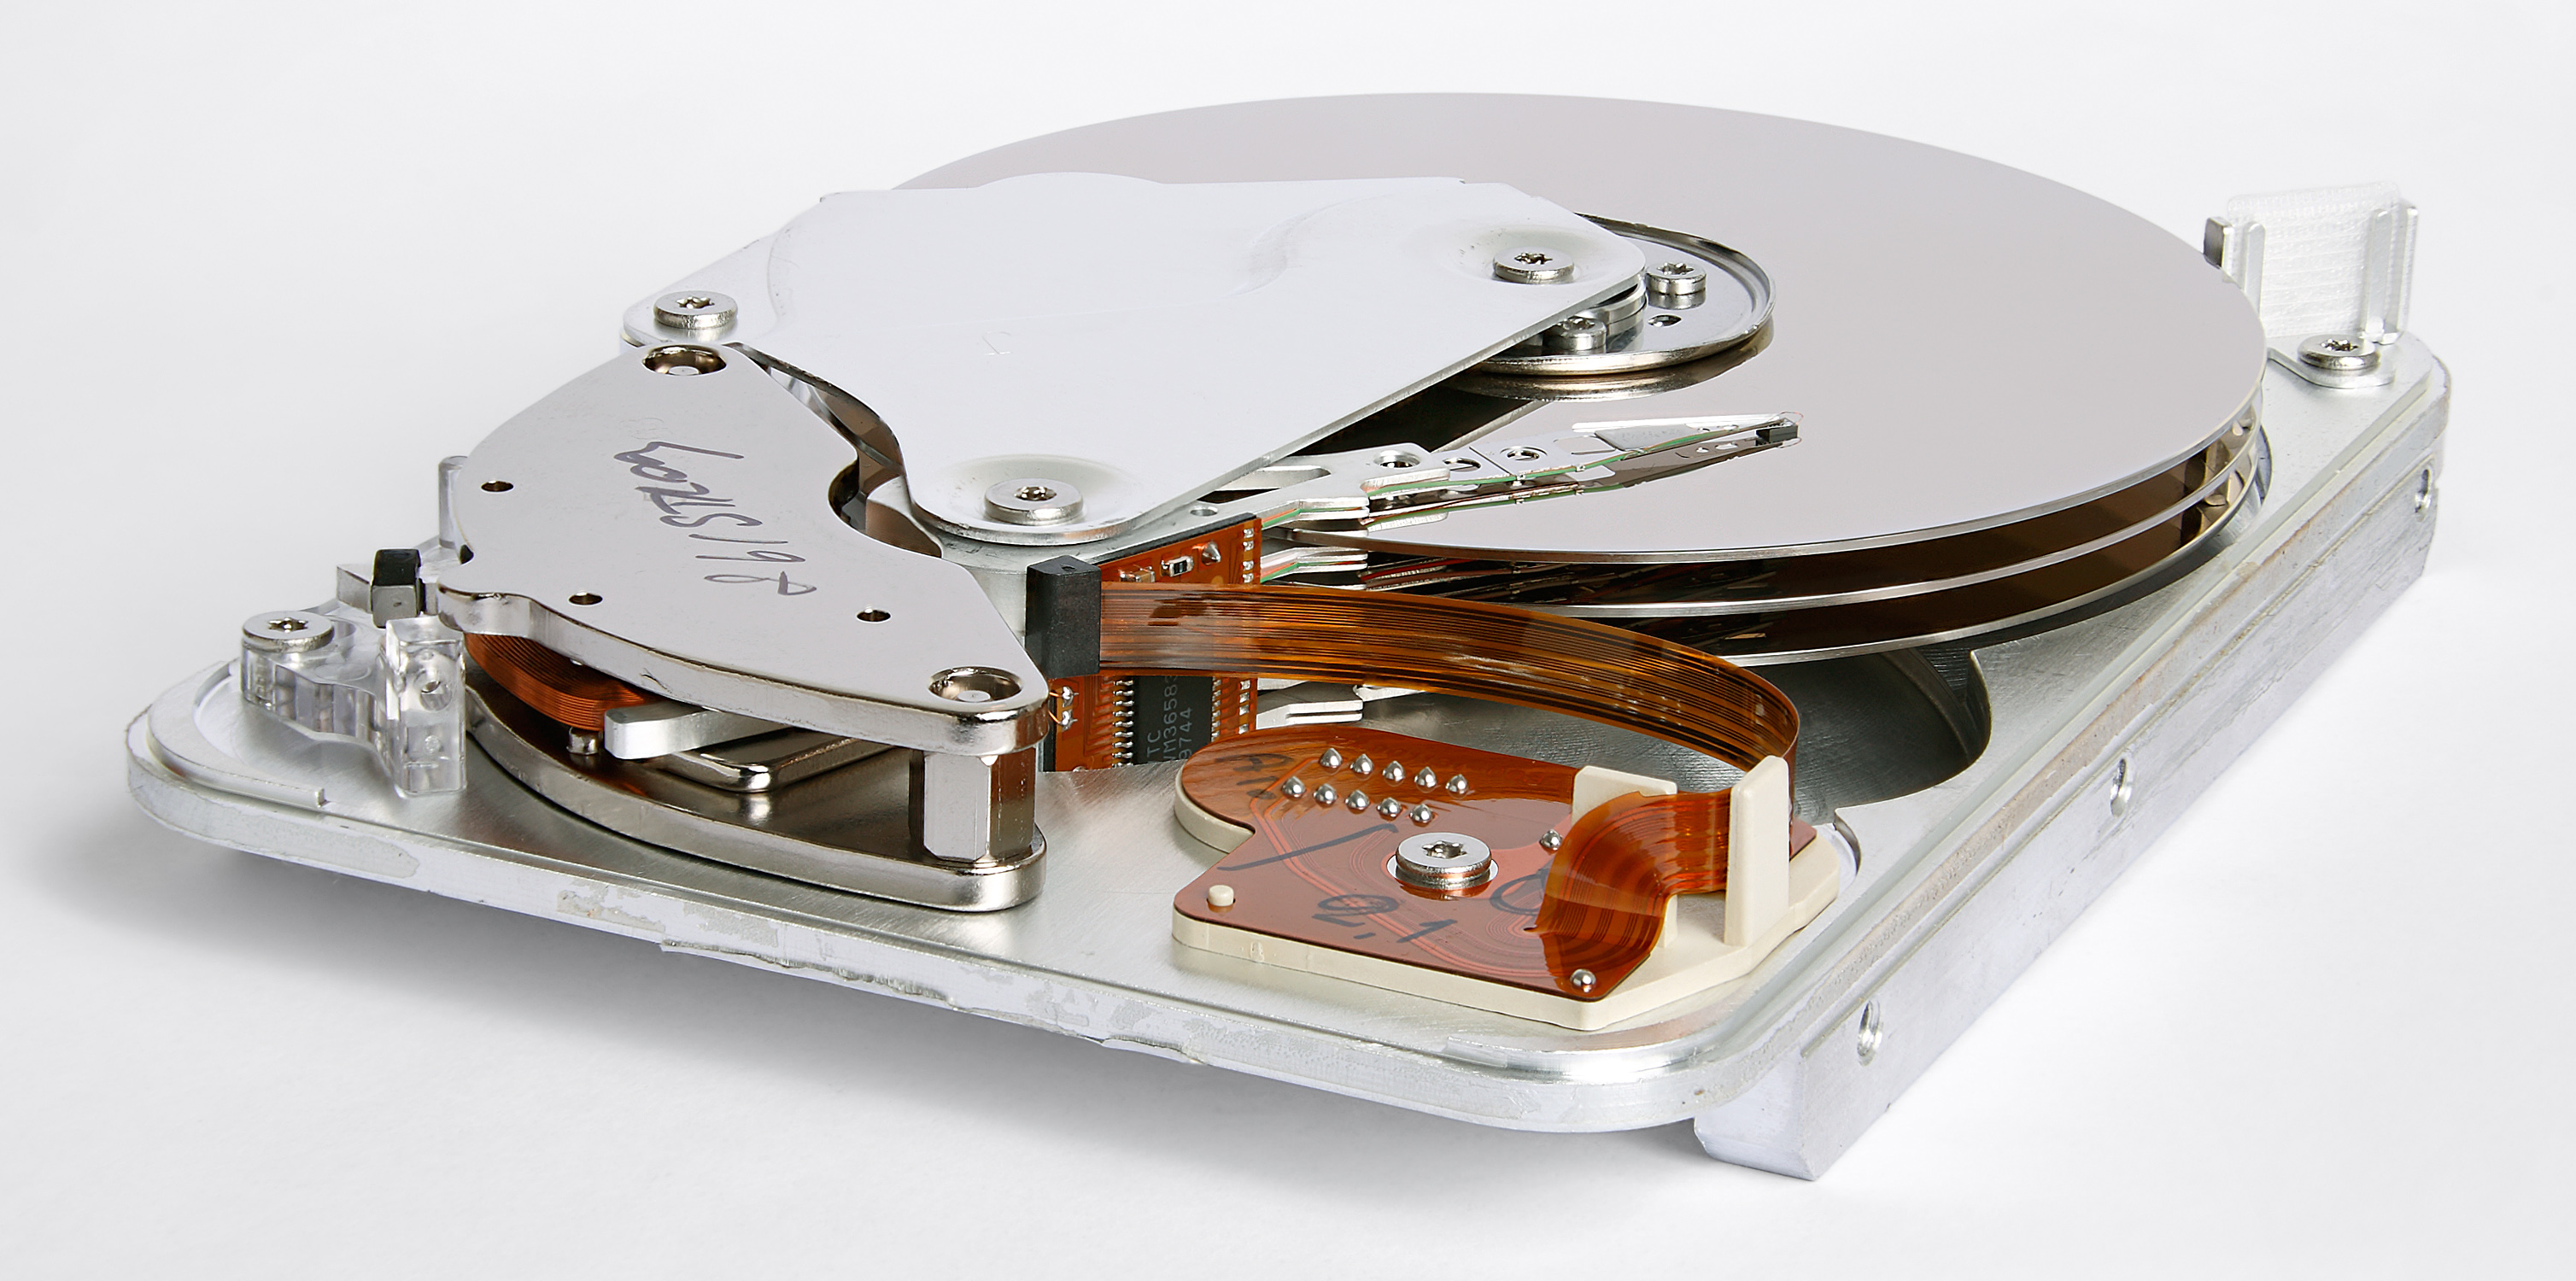
\includegraphics[keepaspectratio,alt={Interno di un Hard Disk Drive: piatti magnetici e testine di lettura/scrittura}]{images/Seagate-ST33232A-hard-disk-inner-view-3421b8.jpg}}
\emph{Fig. --- Anatomia interna di un HDD Seagate: i piatti magnetici
rotanti e il braccio con le testine rendono visibile il vincolo
meccanico che limita la latenza a 3--5 ms.}

\begin{center}\rule{0.5\linewidth}{0.5pt}\end{center}

\subsection{La transizione all'SSD: 30x in un solo
salto}\label{la-transizione-allssd-30x-in-un-solo-salto}

Gli SSD entrarono nel mercato consumer intorno al \textbf{2010},
inizialmente come dispositivi costosi e di piccola capacità, nella forma
fattore di un disco da 2,5'' per poter usare la stessa infrastruttura
meccanica degli HDD. Il cambio non fu graduale: le prime generazioni di
SSD su interfaccia SATA offrirono una riduzione della latency di circa
\textbf{30x} rispetto agli HDD --- da millisecondi a centinaia di
microsecondi. Il risultato fu una ``rivoluzione silenziosa'' che pochi
compresero appieno all'epoca.

\begin{calloutwarning}{Impatto a catena sull’intero stack}

L'accelerazione dello storage non rimase confinata all'hardware. Il
sistema operativo Linux (e altri) nascondeva bug di concorrenza latenti
da oltre vent'anni nel sottosistema di I/O, mai scatenati perché il
disco era troppo lento. Con l'arrivo degli SSD, alcune race condition
diventarono manifeste. Bisognò riscrivere parti del kernel e rivedere
decenni di assunzioni sulla lentezza del disco.

\end{calloutwarning}

\begin{center}\rule{0.5\linewidth}{0.5pt}\end{center}

\subsection{NVMe: un protocollo, non un
dispositivo}\label{nvme-un-protocollo-non-un-dispositivo}

La seconda grande svolta fu lo spostamento degli SSD dal controller SATA
alla connessione diretta al bus \textbf{PCIe} (\emph{PCI Express})
tramite il protocollo \textbf{NVMe} (\emph{Non-Volatile Memory
Express}).

È fondamentale capire che \textbf{NVMe non è un componente hardware}: è
uno \textbf{standard di protocollo} che definisce come un dispositivo di
storage a blocchi deve comportarsi sul bus PCIe. In pratica, un drive
NVMe si presenta al sistema esattamente come qualsiasi altra scheda PCIe
--- una scheda di rete, una GPU --- e il sistema operativo lo riconosce
automaticamente senza driver proprietari.

L'effetto sul collo di bottiglia fu immediato:

{\def\LTcaptype{none} % do not increment counter
\begin{longtable}[]{@{}lll@{}}
\toprule\noalign{}
Interfaccia & Latenza tipica & Bandwidth tipico \\
\midrule\noalign{}
\endhead
\bottomrule\noalign{}
\endlastfoot
HDD SATA/SAS & 3--5 ms & 100--250 MB/s \\
SSD SATA (2015) & 50--200 µs & 500--550 MB/s \\
SSD NVMe Gen 3 (2016+) & 20--100 µs & \textasciitilde3,5 GB/s \\
SSD NVMe Gen 4 (2019+) & 10--50 µs & \textasciitilde7 GB/s \\
SSD NVMe Gen 5 (2022+) & 5--20 µs & 10--14 GB/s \\
\end{longtable}
}

\pandocbounded{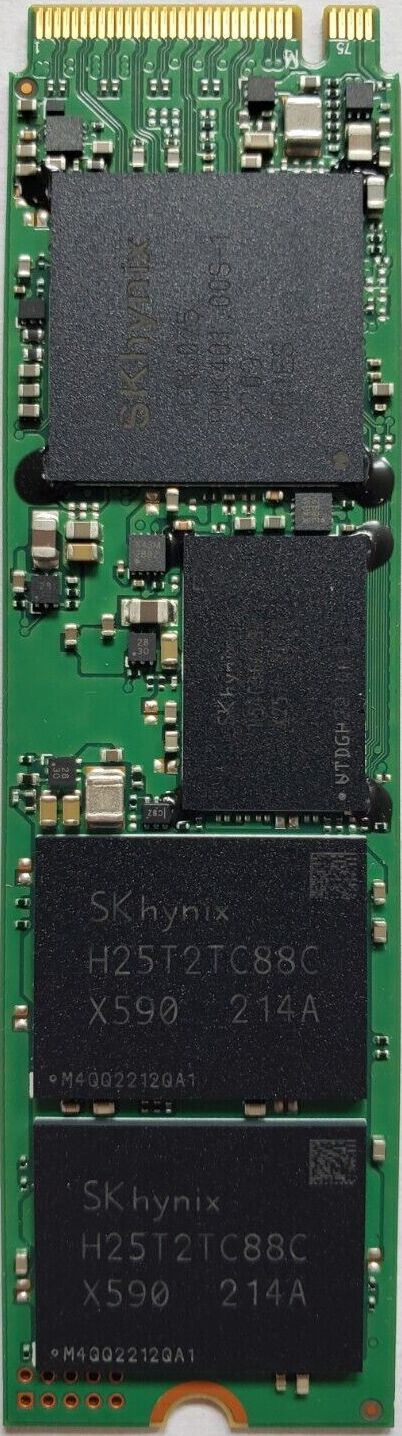
\includegraphics[keepaspectratio,alt={SSD NVMe M.2 2280 da 1 TB}]{images/1TB-2280-NVME-SSD-3504e0.jpg}}
\emph{Fig. --- Un SSD NVMe in formato M.2 2280: la connessione diretta
al bus PCIe elimina il controller SATA e porta la bandwidth a oltre 7
GB/s.}

\begin{callouttip}{Il controller come collo di bottiglia}

Il controller SATA/SAS era un chip hardware interposto tra il drive e la
CPU, utile quando il drive era lento e aveva bisogno di buffering e
command queuing. Con l'SSD, il controller divenne il
\textbf{bottleneck}: rimuovendolo e collegando il drive direttamente al
bus PCIe, si ottenne un guadagno di \textbf{4--5x in bandwidth} e
\textbf{3--4x in latenza} a parità di tecnologia flash.

\end{callouttip}

Ogni drive NVMe usa tipicamente \textbf{4 corsie PCIe} (\emph{lanes}).
La latenza attuale dei drive NVMe enterprise più veloci --- circa 5 µs
--- è a un passo dai 2 µs di InfiniBand, la migliore fabric HPC. Lo
storage, da componente lento, sta diventando ``memoria persistente
lenta''.

\begin{center}\rule{0.5\linewidth}{0.5pt}\end{center}

\section{La Conseguenza Sistemica: PCIe come Collo di
Bottiglia}\label{la-conseguenza-sistemica-pcie-come-collo-di-bottiglia}

Con la rimozione del controller e la connessione diretta al bus PCIe,
l'intero ecosistema dovette adeguarsi. PCIe Gen 3 aveva retto per circa
10 anni, ma improvvisamente divenne il nuovo collo di bottiglia.

La risposta fu una rapida evoluzione degli standard:

\begin{itemize}
\tightlist
\item
  \textbf{PCIe Gen 4} (2019): raddoppia la bandwidth rispetto a Gen 3
\item
  \textbf{PCIe Gen 5} (2021): raddoppia ancora --- \textasciitilde14
  GB/s per drive
\item
  \textbf{PCIe Gen 6 e 7}: in sviluppo
\end{itemize}

\begin{callouttip}{AMD EPYC “Naples” (2017) e le corsie PCIe}

Quando AMD tornò competitiva nel segmento server con la serie EPYC, una
delle sue proposte di valore chiave fu l'offerta di \textbf{128 corsie
PCIe} per socket. La scelta non era casuale: il settore aveva già
compreso che la CPU doveva poter alimentare direttamente i drive NVMe
senza intermediari, e più corsie significava più drive operativi in
parallelo.

\end{callouttip}

Un server tipico con 24 drive NVMe (24 × 4 corsie = 96 corsie) richiede
un numero di corsie PCIe che solo le CPU moderne riescono a fornire. Ciò
ha spinto i produttori a integrare direttamente il controller PCIe nel
die della CPU, eliminando il chip bridge che aggiungeva latenza.

\begin{center}\rule{0.5\linewidth}{0.5pt}\end{center}

\section{Gerarchia della Memoria e la Nuova Posizione dello
SSD}\label{gerarchia-della-memoria-e-la-nuova-posizione-dello-ssd}

La tradizionale gerarchia della memoria è sempre stata:

\begin{verbatim}
Cache L1/L2/L3 (ns) → DRAM (50–100 ns) → Disco (ms)
\end{verbatim}

Con gli SSD NVMe moderni, la gerarchia si è trasformata:

\begin{verbatim}
Cache L1/L2/L3 (ns) → DRAM (50–100 ns) → SSD NVMe (5–20 µs) → HDD (3–5 ms)
\end{verbatim}

Il salto tra DRAM e SSD non è più di 6 ordini di grandezza (come tra ns
e ms), ma di \textbf{2 ordini di grandezza}. Questo ha conseguenze
algoritmiche profonde: strutture dati che prima dovevano risiedere
interamente in memoria --- perché la serializzazione su disco era
proibitiva --- ora possono essere mantenute direttamente sull'SSD.

\begin{callouttip}{RocksDB come caso paradigmatico}

RocksDB (Facebook/Meta) è una libreria che implementa una
\emph{persistent hash table} ottimizzata per SSD. Prima degli SSD
veloci, qualsiasi dato che doveva sopravvivere al riavvio richiedeva
serializzazione su disco con buffer intermedi in memoria. Con RocksDB su
NVMe, si scrivono coppie chiave-valore direttamente su storage
persistente senza gestire esplicitamente buffer o strutture doppie. Le
performance sono abbastanza buone da rendere il pattern accettabile.

\end{callouttip}

\begin{center}\rule{0.5\linewidth}{0.5pt}\end{center}

\subsection{Intel Optane (3D XPoint): La Memoria Persistente che Non
Fu}\label{intel-optane-3d-xpoint-la-memoria-persistente-che-non-fu}

Intel Optane è una tecnologia \textbf{non NAND} che merita menzione,
nonostante Intel l'abbia cancellata nel 2022. Utilizzava una struttura
tridimensionale a giunzioni (\emph{3D Cross-Point}) che permetteva di
memorizzare un bit a ogni incrocio di un reticolo 3D. Le proprietà che
la distinguevano dalle NAND flash:

\begin{itemize}
\tightlist
\item
  \textbf{Latenza quasi simmetrica}: lettura e scrittura avevano tempi
  paragonabili (fattore 3--10x, contro i 6--100x delle NAND)
\item
  \textbf{Endurance molto superiore}: milioni di cicli PE contro i
  migliaia delle NAND TLC
\item
  \textbf{Connessione alla memoria bus}: installabile su slot DIMM
  (\emph{NVDIMM}), non solo su PCIe
\end{itemize}

\begin{calloutdefinition}{NVDIMM — Non-Volatile DIMM}

Standard elettrico introdotto da Intel intorno al 2015 per permettere
l'installazione di moduli di memoria persistente sullo stesso bus dei
moduli DRAM standard. Optane era disponibile in moduli da 512 GB per
slot, consentendo server con \textbf{terabyte di RAM persistente}.

\end{calloutdefinition}

La tecnologia permetteva al processore di fare \emph{tiering}
automatico: i dati caldi residevano in DRAM, quelli tiepidi migrando su
Optane. In termini di latenza, Optane NVMe era intorno ai \textbf{10 µs}
con variazione minima tra lettura e scrittura --- il miglior
avvicinamento alla DRAM come storage persistente mai commercializzato.

I motivi del fallimento furono due: 1. \textbf{Intel attraversava una
crisi interna} e dovette tagliare progetti costosi 2. \textbf{Il
software non era pronto}: i sistemi operativi non sapevano sfruttare il
memory tiering con sufficiente efficienza, e l'NVMe SSD nel frattempo
stava migliorando rapidamente

\begin{calloutnote}{Il problema di sicurezza della memoria persistente}

La persistenza nei DIMM introduce un vettore di attacco imprevisto: un
attaccante fisico che rimuove i moduli può leggerne il contenuto
offline. Intel risolse generando una chiave crittografica casuale
all'avvio, memorizzata in un registro volatile. Tutti i dati scritti
sull'Optane erano cifrati con quella chiave. Se il modulo veniva
rimosso, il registro veniva perso, rendendo inutilizzabile il contenuto
--- simulando il comportamento della DRAM tradizionale.

\end{calloutnote}

\begin{center}\rule{0.5\linewidth}{0.5pt}\end{center}

\section{Asimmetria Lettura/Scrittura negli
SSD}\label{asimmetria-letturascrittura-negli-ssd}

Tutti i dispositivi basati su tecnologia NAND (a differenza di Optane)
presentano una \textbf{asimmetria fondamentale} tra latenza di lettura e
latenza di scrittura.

\begin{calloutdefinition}{Ciclo PE — Program/Erase}

Una cella NAND non può essere riscritta direttamente: prima deve essere
\textbf{cancellata} (\emph{erase}) e poi \textbf{programmata}
(\emph{program}). La cancellazione avviene a livello di blocco (migliaia
di celle), mentre la scrittura avviene a livello di pagina. Questo
genera amplificazione di scrittura e latenza asimmetrica.

\end{calloutdefinition}

{\def\LTcaptype{none} % do not increment counter
\begin{longtable}[]{@{}llll@{}}
\toprule\noalign{}
Tecnologia & Latenza lettura & Latenza scrittura & Rapporto \\
\midrule\noalign{}
\endhead
\bottomrule\noalign{}
\endlastfoot
DRAM & \textasciitilde50--100 ns & \textasciitilde50--100 ns &
\textasciitilde1x (simmetrica) \\
Intel Optane & \textasciitilde6--10 µs & \textasciitilde6--10 µs &
\textasciitilde1--3x \\
SSD NVMe Gen 5 & \textasciitilde20--50 µs & \textasciitilde50--200 µs &
\textasciitilde2--7x \\
SSD SATA (2015) & \textasciitilde50--100 µs & \textasciitilde500 µs--5
ms & \textasciitilde10--100x \\
HDD & \textasciitilde3--5 ms & \textasciitilde3--5 ms &
\textasciitilde1x (simmetrica, ma lenta) \\
\end{longtable}
}

Questa asimmetria è rilevante nelle scelte architetturali: workload
write-intensive richiedono drive con migliore endurance (SLC o MLC), e i
sistemi di storage devono prevedere buffer di scrittura appropriati.

\begin{center}\rule{0.5\linewidth}{0.5pt}\end{center}

\section{Tipologie di Celle NAND e
Endurance}\label{tipologie-di-celle-nand-e-endurance}

Non tutti gli SSD sono uguali: la densità delle celle NAND --- misurata
in bit per cella --- determina un trade-off tra capacità, costo,
prestazioni e vita utile.

\begin{calloutdefinition}{Cicli PE (Program/Erase)}

Ogni cella NAND può essere cancellata e riscritta un numero finito di
volte. Questo numero, detto \emph{PE cycles} o \emph{endurance},
diminuisce all'aumentare dei bit per cella: più stati da distinguere
significano margini elettrici più stretti e usura più rapida.

\end{calloutdefinition}

{\def\LTcaptype{none} % do not increment counter
\begin{longtable}[]{@{}
  >{\raggedright\arraybackslash}p{(\linewidth - 10\tabcolsep) * \real{0.1667}}
  >{\raggedright\arraybackslash}p{(\linewidth - 10\tabcolsep) * \real{0.1667}}
  >{\raggedright\arraybackslash}p{(\linewidth - 10\tabcolsep) * \real{0.1667}}
  >{\raggedright\arraybackslash}p{(\linewidth - 10\tabcolsep) * \real{0.1667}}
  >{\raggedright\arraybackslash}p{(\linewidth - 10\tabcolsep) * \real{0.1667}}
  >{\raggedright\arraybackslash}p{(\linewidth - 10\tabcolsep) * \real{0.1667}}@{}}
\toprule\noalign{}
\begin{minipage}[b]{\linewidth}\raggedright
Tipo
\end{minipage} & \begin{minipage}[b]{\linewidth}\raggedright
Bit/cella
\end{minipage} & \begin{minipage}[b]{\linewidth}\raggedright
PE Cycles tipici
\end{minipage} & \begin{minipage}[b]{\linewidth}\raggedright
Latenza scrittura
\end{minipage} & \begin{minipage}[b]{\linewidth}\raggedright
Costo/GB
\end{minipage} & \begin{minipage}[b]{\linewidth}\raggedright
Caso d'uso
\end{minipage} \\
\midrule\noalign{}
\endhead
\bottomrule\noalign{}
\endlastfoot
\textbf{SLC} & 1 & \textasciitilde50.000--100.000 & \textasciitilde200
µs & Molto alto & Cache, storage ad alta frequenza di scrittura \\
\textbf{MLC (eMLC)} & 2 & \textasciitilde10.000--30.000 &
\textasciitilde600 µs & Alto & Enterprise, workload misto
lettura/scrittura \\
\textbf{TLC} & 3 & \textasciitilde1.000--3.000 & \textasciitilde1--3 ms
& Medio & Standard consumer e enterprise oggi \\
\textbf{QLC} & 4 & \textasciitilde100--1.000 & \textasciitilde5--10 ms &
Basso & Storage freddo, archivio \\
\textbf{PLC} & 5 & \textless100 & \textasciitilde10--20 ms & Molto basso
& Archiviazione pura (\emph{write once}) \\
\end{longtable}
}

\begin{calloutwarning}{SLC come cache interna}

Molti drive TLC e QLC includono una porzione di celle configurate in
modalità SLC come \textbf{buffer di scrittura} interno. Le scritture
iniziali vanno nella cache SLC (molto veloce), poi vengono migrata nel
TLC/QLC in background. Quando il buffer SLC si esaurisce (drive quasi
pieno), le prestazioni di scrittura crollano bruscamente.

\end{calloutwarning}

\begin{center}\rule{0.5\linewidth}{0.5pt}\end{center}

\subsection{Over-provisioning e
precondizionamento}\label{over-provisioning-e-precondizionamento}

Un SSD da 4 TB potrebbe internamente contenere 6--8 TB di celle NAND. La
capacità ``nascosta'' oltre quella esposta serve a due scopi:

\begin{enumerate}
\def\labelenumi{\arabic{enumi}.}
\tightlist
\item
  \textbf{Wear leveling}: il controller distribuisce le scritture
  uniformemente su tutte le celle per evitare che alcune si esauriscano
  prima di altre. Avere celle di riserva moltiplica la vita effettiva
  del drive.
\item
  \textbf{Performance}: il controller usa lo spazio libero per
  ottimizzare le operazioni di garbage collection e riorganizzazione
  interna.
\end{enumerate}

\begin{calloutwarning}{Il “precondizionamento” e la barra rossa}

Quando un drive supera circa il \textbf{90\% di riempimento}, le
prestazioni degradano significativamente. Il controller ha meno spazio
libero per fare wear leveling e ottimizzazione. macOS e Windows mostrano
la barra di utilizzo in rosso proprio a questo punto --- non per
indicare che il disco è quasi pieno in senso assoluto, ma per segnalare
che le \textbf{prestazioni stanno per peggiorare}. Regola pratica:
mantenere un drive SSD sotto il 75--80\% per preservare le prestazioni.

\end{calloutwarning}

\begin{center}\rule{0.5\linewidth}{0.5pt}\end{center}

\section{Il Peccato Imperdonabile: Perdere i
Dati}\label{il-peccato-imperdonabile-perdere-i-dati}

Prima di affrontare le soluzioni tecniche, il professore pone il
principio cardine di tutto il dominio storage:

\begin{calloutwarning}{La regola fondamentale dello storage}

In IT esistono eventi gravi ma recuperabili --- un server che si rompe,
una rete che cade. Esiste però \textbf{un solo peccato imperdonabile}:
\textbf{perdere i dati}. Tutto il resto si ripristina; i dati persi non
tornano.

\end{calloutwarning}

Questo non è un fatto tecnologico, è un fatto organizzativo e culturale.
Qualsiasi sistema di storage deve essere progettato partendo da questo
assioma: il disco \emph{può} e \emph{prima o poi} \textbf{fallirà}. La
domanda non è ``se'' un drive si romperà, ma ``quando''.

\begin{callouttip}{Il datacenter di Bruxelles}

Un cloud provider installò due datacenter nello stesso isolato di
Bruxelles, in edifici separati con linee elettriche indipendenti. I due
datacenter erano configurati come backup l'uno dell'altro. Un incendio
di proporzioni eccezionali distrusse entrambi gli edifici. Risultato:
perdita totale dei dati. La normativa europea richiede oggi una distanza
minima di \textbf{11--12 km} tra datacenter usati per la replica dei
dati, proprio per mitigare rischi di questo tipo (inondazioni, incendi,
guasti di rete elettrica locali).

\end{callouttip}

\begin{center}\rule{0.5\linewidth}{0.5pt}\end{center}

\section{RAID: Ridondanza attraverso
l'Aggregazione}\label{raid-ridondanza-attraverso-laggregazione}

\textbf{RAID} (\emph{Redundant Array of Inexpensive Disks}) nacque negli
anni '80 non come soluzione di backup, ma come risposta a un problema
economico: un drive di grande capacità costava molto più di due drive
più piccoli. L'idea era aggregare drive economici in un unico volume
logico, compensando la loro minore affidabilità con la ridondanza.

Il meccanismo comune a tutti i livelli RAID è il \textbf{parallelismo}:
se ho due drive e devo scrivere due blocchi, posso inviarli
contemporaneamente ai due drive, eseguendo due scritture al costo
temporale di una.

\begin{center}\rule{0.5\linewidth}{0.5pt}\end{center}

\subsection{RAID 0 --- Striping (nessuna
ridondanza)}\label{raid-0-striping-nessuna-ridondanza}

Il \textbf{RAID 0} non è propriamente un RAID nel senso di ridondanza:
si tratta di \textbf{striping}, cioè della distribuzione dei dati su più
drive per presentare al sistema un singolo volume logico più grande. I
blocchi vengono alternati tra i drive: blocco 0 → drive A, blocco 1 →
drive B, blocco 2 → drive A, ecc.

Il vantaggio è doppio: capacità aggregata e potenziale di
leggere/scrivere in parallelo dai due drive. Lo svantaggio è totale
assenza di protezione: la perdita di un qualsiasi drive causa la perdita
dell'intero volume.

\begin{center}\rule{0.5\linewidth}{0.5pt}\end{center}

\subsection{RAID 1 --- Mirror (specchio)}\label{raid-1-mirror-specchio}

Il \textbf{RAID 1} è la forma più intuitiva di ridondanza: ogni blocco è
scritto identicamente su due drive. In caso di guasto di un drive, si
opera sul secondo senza interruzioni. Il prezzo da pagare è la
\textbf{capacità effettiva dimezzata}: due drive da 4 TB danno 4 TB
utilizzabili.

In compenso, le letture possono essere distribuite sui due drive,
migliorando il throughput in lettura. La fase di \emph{rebuild} (copia
del drive funzionante sul nuovo drive) non richiede di portare il volume
offline.

\begin{center}\rule{0.5\linewidth}{0.5pt}\end{center}

\subsection{RAID 5 --- Parità distribuita con
XOR}\label{raid-5-parituxe0-distribuita-con-xor}

Il \textbf{RAID 5} usa un meccanismo matematico elegante per ottenere
ridondanza con un overhead di \textbf{1/N} anziché del 50\% del RAID 1.

\begin{callouttheorem}{La proprietà XOR che rende possibile RAID 5}

L'operazione \textbf{XOR} (\emph{OR esclusivo}) ha una proprietà
fondamentale: se \(A \oplus B = C\), allora conoscendo due qualsiasi dei
tre valori si può ricostruire il terzo: \(A = B \oplus C\),
\(B = A \oplus C\).

In RAID 5 con 3 drive, si memorizzano i dati sui drive A e B, e il loro
XOR sul drive C (chiamato blocco di parità). Se uno dei tre drive
fallisce, si ricostruisce il suo contenuto calcolando lo XOR degli altri
due.

\end{callouttheorem}

Con \(N\) drive in RAID 5: - \textbf{Capacità utile}: \((N-1)/N\) del
totale (con 3 drive: 66\%, con 6 drive: 83\%) - \textbf{Tolleranza}:
perdita di \textbf{1 drive} - \textbf{Rebuild}: richiede di portare il
volume offline, ricalcolare tutti i blocchi di parità

Il costo nascosto del RAID 5 è il \textbf{degraded mode}: quando un
drive fallisce e si aspetta la sostituzione, il sistema deve eseguire la
ricostruzione di ogni blocco mancante on-the-fly, aumentando la latenza
di lettura. Se un secondo drive fallisce durante il rebuild, si perde
tutto.

\begin{center}\rule{0.5\linewidth}{0.5pt}\end{center}

\subsection{RAID 6 --- Doppia parità}\label{raid-6-doppia-parituxe0}

Il \textbf{RAID 6} estende il RAID 5 con \textbf{doppia parità} (usando
algoritmi matematici più sofisticati dell'XOR semplice, basati sui campi
di Galois). Questo permette di:

\begin{itemize}
\tightlist
\item
  Tollerare la perdita di \textbf{2 drive} simultaneamente
\item
  Rimanere \textbf{online} in modalità degradata con 1 drive guasto
  durante il rebuild
\end{itemize}

Il costo in capacità è leggermente superiore al RAID 5 (overhead di 2/N
anziché 1/N), ma il guadagno in affidabilità è significativo.

\textbf{RAID 6 è oggi lo standard de facto} nei sistemi di storage,
preferito al RAID 5 perché il rischio di guasto di un secondo drive
durante il lungo processo di rebuild di un array moderno (ore su drive
da decine di TB) è concreto.

\begin{center}\rule{0.5\linewidth}{0.5pt}\end{center}

\subsection{Confronto riepilogativo
RAID}\label{confronto-riepilogativo-raid}

{\def\LTcaptype{none} % do not increment counter
\begin{longtable}[]{@{}
  >{\raggedright\arraybackslash}p{(\linewidth - 10\tabcolsep) * \real{0.1667}}
  >{\raggedright\arraybackslash}p{(\linewidth - 10\tabcolsep) * \real{0.1667}}
  >{\raggedright\arraybackslash}p{(\linewidth - 10\tabcolsep) * \real{0.1667}}
  >{\raggedright\arraybackslash}p{(\linewidth - 10\tabcolsep) * \real{0.1667}}
  >{\raggedright\arraybackslash}p{(\linewidth - 10\tabcolsep) * \real{0.1667}}
  >{\raggedright\arraybackslash}p{(\linewidth - 10\tabcolsep) * \real{0.1667}}@{}}
\toprule\noalign{}
\begin{minipage}[b]{\linewidth}\raggedright
Livello
\end{minipage} & \begin{minipage}[b]{\linewidth}\raggedright
Drive minimi
\end{minipage} & \begin{minipage}[b]{\linewidth}\raggedright
Capacità utile
\end{minipage} & \begin{minipage}[b]{\linewidth}\raggedright
Drive tollerati
\end{minipage} & \begin{minipage}[b]{\linewidth}\raggedright
Online con 1 guasto
\end{minipage} & \begin{minipage}[b]{\linewidth}\raggedright
Meccanismo
\end{minipage} \\
\midrule\noalign{}
\endhead
\bottomrule\noalign{}
\endlastfoot
RAID 0 & 2 & 100\% & 0 & No & Striping \\
RAID 1 & 2 & 50\% & 1 & Sì & Mirroring \\
RAID 5 & 3 & \((N-1)/N\) & 1 & Degraded & Parità XOR \\
RAID 6 & 4 & \((N-2)/N\) & 2 & Sì (con 1) & Doppia parità \\
\end{longtable}
}

\begin{calloutnote}{Chi implementa il RAID?}

Storicamente, il RAID era implementato dal \textbf{controller hardware}
del disco: il chip interposto tra i drive e la CPU esponeva un singolo
volume logico al sistema operativo. Con la transizione a NVMe (che
elimina il controller), il RAID deve essere implementato dal
\textbf{sistema operativo} (Linux \texttt{mdadm}, Windows Storage
Spaces) o da software dedicato. L'OS è perfettamente in grado di farlo,
ma la transizione ha richiesto adattamento nei workflow di
amministrazione.

\end{calloutnote}

\begin{center}\rule{0.5\linewidth}{0.5pt}\end{center}

\section{Verso le Architetture di Storage
Distribuite}\label{verso-le-architetture-di-storage-distribuite}

La lezione si chiude con un'anticipazione: il singolo server con RAID
non è sufficiente per le esigenze dei datacenter moderni. L'evoluzione
naturale porta alle \textbf{architetture di storage centralizzato e
distribuito}, che saranno trattate nelle lezioni successive:

\begin{itemize}
\tightlist
\item
  \textbf{SAN} (\emph{Storage Area Network}): storage condiviso
  accessibile via rete dedicata
\item
  \textbf{NAS} (\emph{Network Attached Storage}): file system condiviso
  via rete standard
\item
  \textbf{HCI} (\emph{Hyper-Converged Infrastructure}): storage
  distribuito che usa i drive locali dei server, con replicazione
  software a \textbf{3 copie} (overhead 3x, ma proprietà di
  disponibilità superiori)
\end{itemize}

\begin{calloutnote}{Sintesi della lezione}

La transizione da HDD a SSD NVMe è una delle rivoluzioni più
sottovalutate dell'informatica degli ultimi 15 anni. Ha ridotto la
latenza di storage da millisecondi a microsecondi, trasformando il disco
da componente lento a quasi-memoria persistente. Questa trasformazione
ha costretto a riprogettare controller, bus PCIe, CPU, sistemi operativi
e architetture software. Il principio guida di tutto lo storage rimane
invariato: \textbf{perdere i dati è imperdonabile}, e ogni scelta
tecnologica --- dal tipo di cella NAND al livello RAID --- ruota attorno
alla massimizzazione dell'affidabilità al minor costo possibile.

\end{calloutnote}

\newpage

\chapter{Storage: Architetture e
Servizi}\label{storage-architetture-e-servizi}

La lezione parte da un'osservazione apparentemente banale: il termine
\emph{disk drive} è ormai un anacronismo. I moderni dispositivi di
storage non contengono più dischi rotanti, eppure continuiamo a
chiamarli così --- esattamente come l'icona del floppy disk campeggia
ancora sul pulsante ``Salva'' di moltissime applicazioni. Questo è un
caso esemplare del \textbf{principio di sostituzione}: quando si evolve
una tecnologia, spesso si mantiene il form factor precedente per
compatibilità con l'infrastruttura esistente, anche quando il nuovo
dispositivo non ne ha più bisogno.

\begin{center}\rule{0.5\linewidth}{0.5pt}\end{center}

\section{Form Factor e Densità dello
Storage}\label{form-factor-e-densituxe0-dello-storage}

\subsection{Il form factor nel
datacenter}\label{il-form-factor-nel-datacenter}

Nei server enterprise il form factor più diffuso rimane quello da
\textbf{2.5 pollici}, pensato originariamente per contenere un disco
rotante. Oggi in quello stesso alloggiamento si inserisce un SSD, che
non ha alcun bisogno di quella forma. Il motivo è semplice: tutta
l'infrastruttura dei server --- backplane, connettori, cage --- è stata
progettata attorno a quel formato e sostituirla ha un costo elevato.

\begin{callouttip}{Il principio del calesse e dell’auto}

Le prime automobili avevano le stesse dimensioni dei calessi a cavallo,
non per necessità tecnica, ma perché strade, rimesse e abitudini erano
calibrate sul vecchio standard. Lo stesso vale per i disk drive nei
server.

\end{callouttip}

\subsection{Il form factor Ruler}\label{il-form-factor-ruler}

L'evoluzione verso lo storage solid state ha però spinto a progettare
form factor nativi per gli SSD. Il più rilevante è il \textbf{Ruler}
(\emph{righello}), un dispositivo lungo e stretto che ottimizza:

\begin{itemize}
\tightlist
\item
  \textbf{Dissipazione del calore}: il form factor circolare del disco
  era efficiente per far ruotare un piatto, ma è subottimale per
  dissipare il calore generato dai chip flash. Il ruler ha superfici
  laterali maggiori che migliorano il flusso d'aria.
\item
  \textbf{Densità}: più ruler possono essere impilati verticalmente in
  un singolo rack unit. Intel aveva dimostrato già circa otto anni fa un
  sistema nell'ordine del \textbf{petabyte in 1U} usando circa 24 moduli
  ruler (numero citato a memoria dal professore, da prendere come ordine
  di grandezza).
\end{itemize}

\pandocbounded{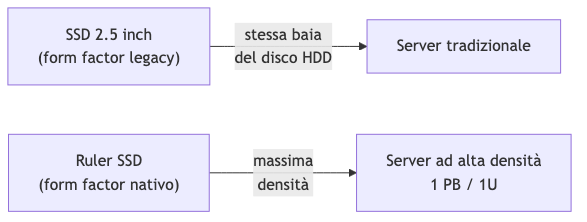
\includegraphics[keepaspectratio,alt={Diagramma Mermaid}]{images/mermaid-lezione-11-storage-architetture-e-servizi-01.png}}
\emph{Fig. --- Confronto tra form factor legacy (2.5'') e Ruler per
storage solid state.}

Il ruler può essere installato con o senza dissipatore integrato: la
versione con dissipatore (\emph{wing}) è leggermente più spessa ma
garantisce prestazioni termiche superiori. La stessa logica è già
presente nei laptop sotto forma di moduli \textbf{M.2}, che sono
essenzialmente dei ruler in miniatura.

\pandocbounded{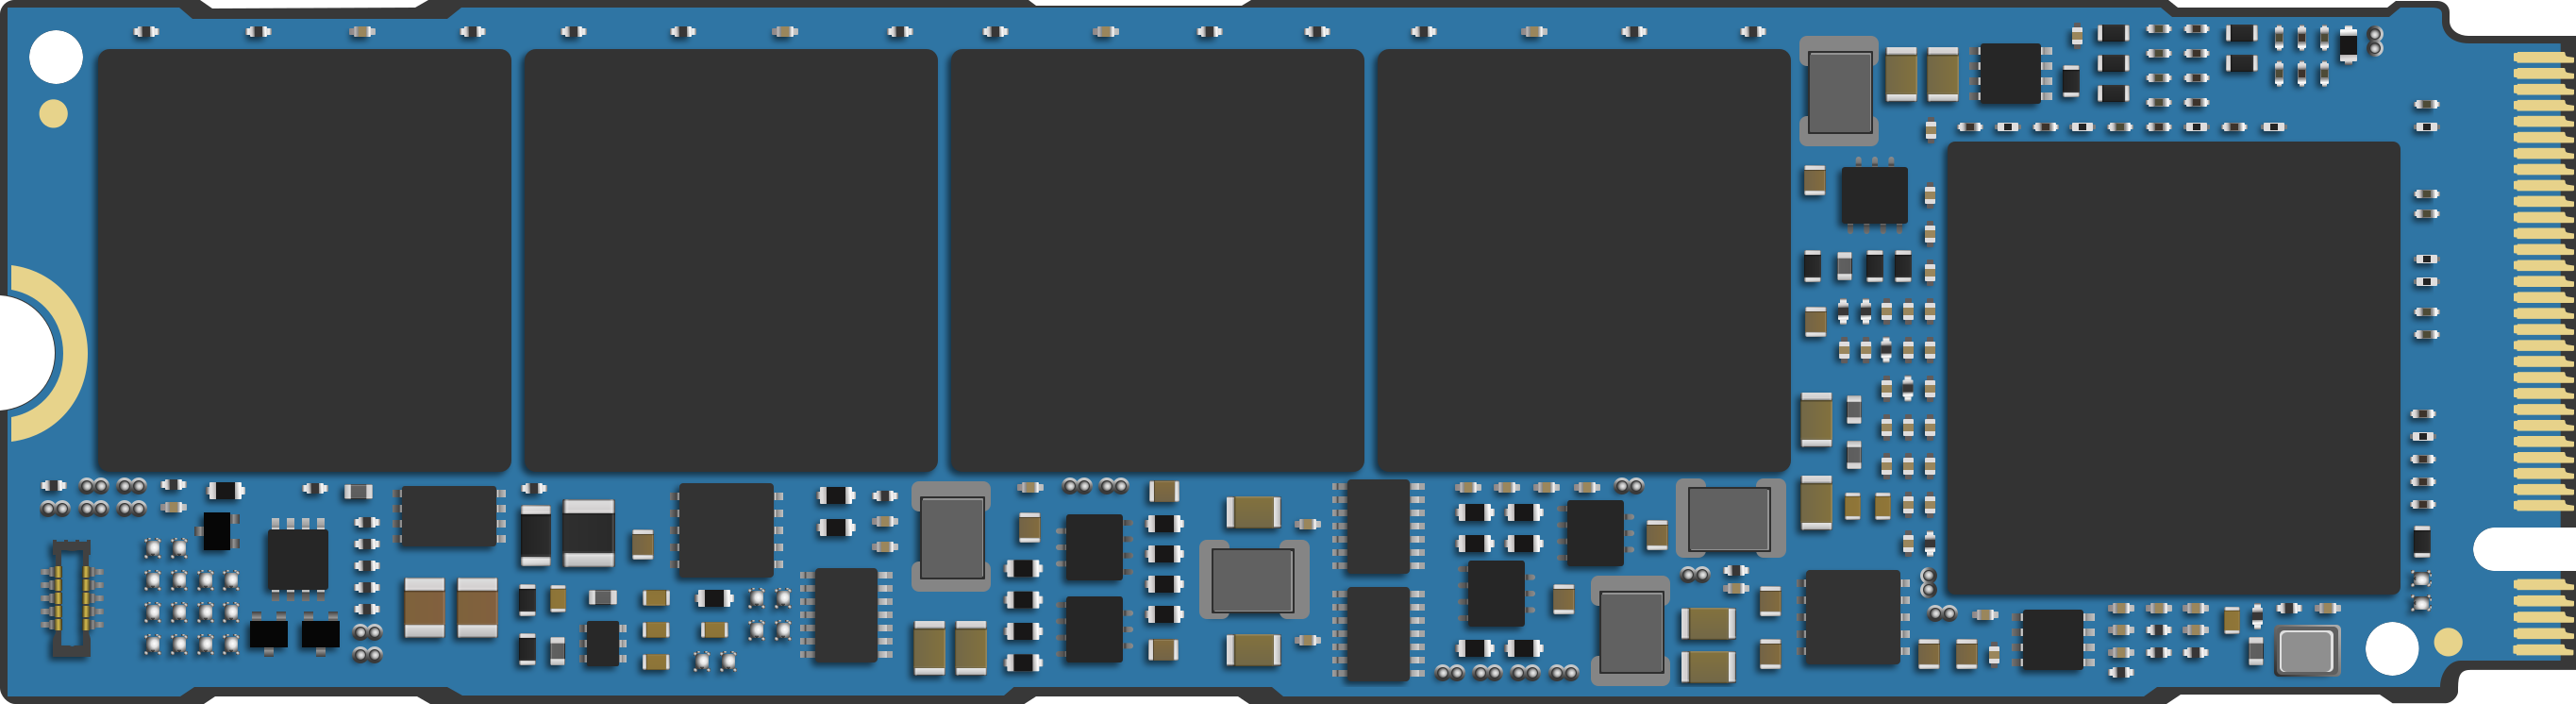
\includegraphics[keepaspectratio,alt={Modulo SSD M.2 --- il form factor ruler dei laptop}]{images/SSD-M-2-8e6d73.png}}
\emph{Fonte: Wikimedia Commons --- Un modulo SSD M.2: forma allungata
identica al principio del Ruler, progettata per massimizzare la densità
nei laptop.}

\begin{center}\rule{0.5\linewidth}{0.5pt}\end{center}

\section{Aggregare lo Storage: RAID e File
System}\label{aggregare-lo-storage-raid-e-file-system}

\subsection{Riepilogo RAID}\label{riepilogo-raid}

Il punto di partenza per costruire uno storage di livello datacenter è
\textbf{aggregare più dischi fisici} in un'unità logica più capace e
resiliente. La tecnologia alla base è il {[}{[}RAID{]}{]}
(\emph{Redundant Array of Inexpensive Disks}).

\begin{calloutwarning}{La perdita di dati è il peccato imperdonabile}

In un datacenter la perdita di dati è inaccettabile. Un utente può
tollerare un'interruzione del servizio --- il dato è irraggiungibile per
un po', è fastidioso ma forgivable. Ma se il dato viene distrutto, la
responsabilità legale e reputazionale è enorme. Ogni scelta
architetturale sullo storage deve partire da questa premessa.

\end{calloutwarning}

Il \textbf{RAID 6} è oggi la scelta più comune in ambito enterprise,
perché permette di perdere un disco e \textbf{sostituirlo a caldo}
(\emph{hot swap}) mentre il sistema continua a operare, ricostruendo i
dati in background. Con RAID 5, invece, la perdita di un disco richiede
di portare offline lo storage per la ricostruzione.

Il costo dello storage in RAID non è solo il costo dei dischi fisici:
include anche lo \textbf{spazio ridondante} necessario alla protezione,
e tutta l'infrastruttura di gestione.

\subsection{File system e RAID}\label{file-system-e-raid}

Una domanda ricorrente: aggregare più dischi via RAID richiede un file
system speciale? La risposta è no. Su Linux, si può configurare RAID con
\textbf{LVM} e formattare il volume risultante con un qualsiasi file
system standard (ext4, XFS, ecc.). Il RAID opera a livello di blocco,
trasparente al file system.

Tuttavia, se il sistema deve gestire \textbf{accessi altamente
concorrenti} da molti processi paralleli --- come in ambito HPC
(\emph{High Performance Computing}) --- il file system standard diventa
il collo di bottiglia. In quel caso si usano \textbf{file system
paralleli}: GFS, GPFS, Lustre e simili, progettati per supportare
concorrenza massiva. Per uso aziendale ordinario (document sharing,
email) un file system standard è sufficiente.

\begin{center}\rule{0.5\linewidth}{0.5pt}\end{center}

\section{Servizi Richiesti allo Storage
Moderno}\label{servizi-richiesti-allo-storage-moderno}

Prima di scegliere un'architettura, è fondamentale capire quali servizi
uno storage di livello datacenter deve offrire. Non si tratta solo di
esporre blocchi su una rete.

\subsection{Deduplicazione}\label{deduplicazione}

Se invio un allegato da 10 MB a 1000 persone nella stessa
organizzazione, uno storage intelligente non conserva 1000 copie
identiche: ne mantiene \textbf{una sola}, registrando solo i
riferimenti. La deduplicazione riduce drasticamente lo spazio occupato,
perché gli utenti tendono a duplicare i file molto più di quanto si
pensi.

\subsection{Compressione}\label{compressione}

La compressione non serve solo a risparmiare spazio: i dati compressi
sono più piccoli, quindi il trasferimento da disco a memoria richiede
\textbf{meno I/O}. Anche con i moderni SSD veloci, la compressione
migliora il throughput, con un piccolo overhead CPU per la
decompressione. Il trade-off è quasi sempre favorevole alla
compressione.

\subsection{Sicurezza}\label{sicurezza}

Uno storage enterprise deve offrire: - \textbf{Encryption at rest}: i
dati sono cifrati quando scritti sul disco, ma decifrati in memoria
durante l'uso. - \textbf{ACL} (\emph{Access Control List}): controllo di
accesso a livello di volume o file. - \textbf{Secure erase}: quando un
file viene cancellato, i blocchi vengono effettivamente sovrascritti per
impedire recupero non autorizzato.

\subsection{Snapshot}\label{snapshot}

Uno \textbf{snapshot} è una fotografia dello stato di un volume in un
preciso istante. Se qualcosa va storto --- un aggiornamento software
rovinato, un ransomware, un errore umano --- si può ripristinare il
volume a quel punto esatto. Nei sistemi enterprise questa operazione
avviene senza interrompere il servizio (tecnica copy-on-write).

\pandocbounded{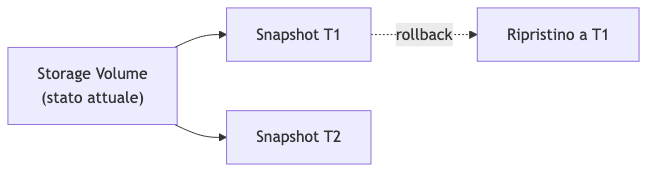
\includegraphics[keepaspectratio,alt={Diagramma Mermaid}]{images/mermaid-lezione-11-storage-architetture-e-servizi-02.png}}
\emph{Fig. --- Meccanismo di snapshot: il volume può essere ripristinato
a qualsiasi stato precedente catturato.}

Tutti questi servizi --- deduplicazione, compressione, sicurezza,
snapshot, e altri --- rendono la gestione dello storage complessa. Per
questo ha senso \textbf{centralizzare} lo storage, svincolarlo dai
singoli server, e affidarlo a un sistema specializzato che li offra in
modo uniforme a tutta l'infrastruttura.

\begin{center}\rule{0.5\linewidth}{0.5pt}\end{center}

\section{Storage Area Network (SAN)}\label{storage-area-network-san}

\subsection{Architettura}\label{architettura}

La \textbf{SAN} (\emph{Storage Area Network}) è l'architettura di
storage più diffusa nei datacenter enterprise. L'idea è separare
fisicamente lo storage dai server di calcolo e collegarli tramite una
rete dedicata ad alte prestazioni.

\pandocbounded{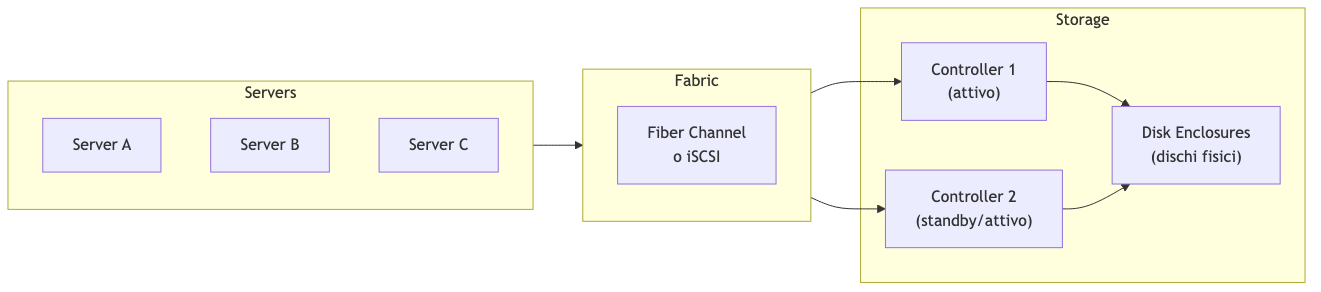
\includegraphics[keepaspectratio,alt={Diagramma Mermaid}]{images/mermaid-lezione-11-storage-architetture-e-servizi-03.png}}
\emph{Fig. --- Architettura SAN: i server accedono allo storage tramite
fabric dedicato verso controller ridondanti.}

\pandocbounded{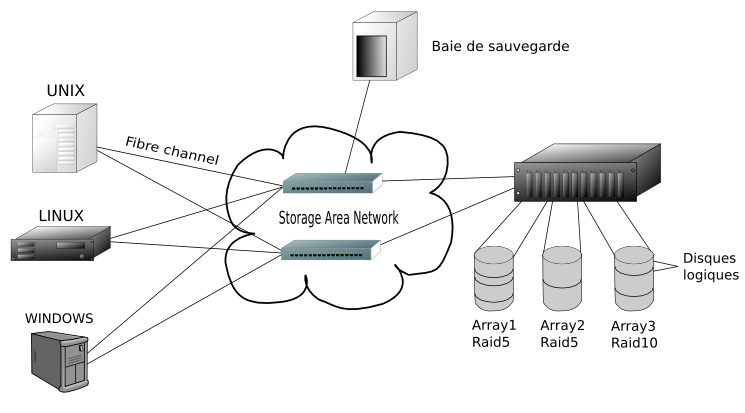
\includegraphics[keepaspectratio,alt={Schema di un'architettura SAN reale}]{images/Sch-ma-SAN-193f9c.png}}
\emph{Fonte: Wikimedia Commons --- Esempio di architettura SAN con
server, switch Fiber Channel e array di storage.}

I componenti chiave sono:

\begin{itemize}
\tightlist
\item
  \textbf{Fabric}: rete dedicata allo storage. Il protocollo
  tradizionale è \textbf{Fiber Channel} (FC), che trasporta blocchi di
  dati su fibra ottica. In alternativa si usa \textbf{iSCSI}, che
  incapsula il protocollo SCSI su Ethernet.
\item
  \textbf{HBA} (\emph{Host Bus Adapter}): scheda nel server che annuncia
  al sistema operativo un disco locale, anche se fisicamente quel disco
  si trova nello storage remoto. Per il SO è trasparente.
\item
  \textbf{Controller}: il cervello dello storage. Riceve le richieste di
  blocchi dai server, gestisce la mappatura sui dischi fisici e
  restituisce i dati. Viene tipicamente duplicato (active/active o
  active/passive) per resistenza ai guasti.
\item
  \textbf{Disk Enclosure}: lo chassis fisico che contiene i dischi,
  collegato ai controller.
\end{itemize}

\subsection{LUN --- Logical Unit Number}\label{lun-logical-unit-number}

Lo storage fisico viene ``affettato'' in unità logiche chiamate
\textbf{LUN} (\emph{Logical Unit Number}), o \emph{logical units}. Una
LUN è un disco virtuale: ha una certa dimensione, è mappata su blocchi
fisici interni allo storage (sopra uno strato RAID), e viene esposta ai
server come se fosse un disco locale.

\pandocbounded{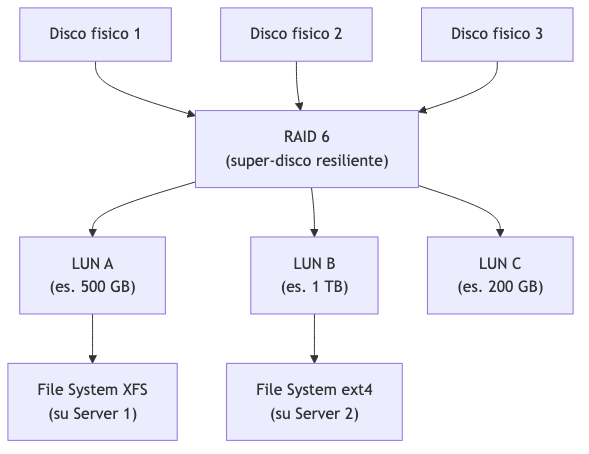
\includegraphics[keepaspectratio,alt={Diagramma Mermaid}]{images/mermaid-lezione-11-storage-architetture-e-servizi-04.png}}
\emph{Fig. --- Gerarchia SAN: dai dischi fisici al RAID, dalle LUN ai
file system sui server.}

\subsection{Vantaggi e limitazioni della
SAN}\label{vantaggi-e-limitazioni-della-san}

Il vantaggio principale della SAN è la \textbf{centralizzazione}: un
team dedicato gestisce tutto lo storage per l'intera infrastruttura, con
backup, ridondanza e servizi avanzati in un solo punto.

\begin{calloutwarning}{Il collo di bottiglia con SSD ad alte prestazioni}

La SAN classica nasce con i dischi meccanici, dove la rete Fiber Channel
era sempre più veloce del disco. Con gli SSD NVMe moderni, capaci di 16
GB/s ciascuno, l'equazione si capovolge: se si aggregano decine di SSD
nello stesso storage, la banda del fabric diventa il collo di bottiglia.
Questo ha spinto allo sviluppo di architetture alternative.

\end{calloutwarning}

\begin{center}\rule{0.5\linewidth}{0.5pt}\end{center}

\section{NAS --- Network Attached
Storage}\label{nas-network-attached-storage}

\subsection{Differenze fondamentali da
SAN}\label{differenze-fondamentali-da-san}

La \textbf{NAS} (\emph{Network Attached Storage}) adotta un approccio
diverso: invece di esporre blocchi grezzi ai server, espone direttamente
\textbf{file e directory} tramite protocolli di file system remoti.

{\def\LTcaptype{none} % do not increment counter
\begin{longtable}[]{@{}lll@{}}
\toprule\noalign{}
Caratteristica & SAN & NAS \\
\midrule\noalign{}
\endhead
\bottomrule\noalign{}
\endlastfoot
Livello di astrazione & Blocchi (raw) & File e directory \\
Protocollo & Fiber Channel, iSCSI & NFS, SMB \\
Rete & Fabric dedicato & Rete Ethernet standard \\
File system & Gestito dal server & Gestito dallo storage \\
Memory mapping & Supportato & Non supportato \\
Latenza & Bassa & Media \\
\end{longtable}
}

I due protocolli NAS più comuni sono: - \textbf{NFS} (\emph{Network File
System}): standard Unix/Linux, ancora dominante nei datacenter. -
\textbf{SMB} (\emph{Server Message Block}): nato in ambito Microsoft,
oggi disponibile su tutte le piattaforme.

\subsection{Memory Mapping e perché
conta}\label{memory-mapping-e-perchuxe9-conta}

\begin{calloutdefinition}{Memory Mapping}

Il \emph{memory mapping} è una tecnica che sfrutta il meccanismo di
paginazione della CPU: un file viene ``mappato'' nello spazio di
indirizzamento del processo, e gli accessi ai byte del file vengono
gestiti direttamente dalla MMU hardware come page fault. Il kernel
carica automaticamente i blocchi necessari dal disco in memoria.

\end{calloutdefinition}

Il memory mapping è oggi dominante --- Windows e Linux lo usano entrambi
come base del loro I/O su file. È enormemente più efficiente rispetto
alle API tradizionali (\texttt{open}/\texttt{seek}/\texttt{read}) per
accessi casuali, perché sfrutta il supporto hardware anziché chiamate di
sistema ripetute.

Ebbene, \textbf{il memory mapping funziona su SAN, ma non su NAS}. Un
file system remoto NAS non supporta \texttt{mmap()}. Questo rende la SAN
l'unica scelta per applicazioni che richiedono accesso casuale ad alta
performance (database, algoritmi analitici, virtual machine).

\subsection{Quando usare NAS}\label{quando-usare-nas}

La NAS è adatta per: - \textbf{Backup} e archiviazione -
\textbf{Document store} (analoga a OneDrive/SharePoint interno) -
Qualsiasi workload con accesso prevalentemente sequenziale

\begin{calloutwarning}{Complessità di integrazione degli ACL}

Il principale problema pratico della NAS è integrare il modello di
sicurezza: gli ACL del file system remoto devono essere mappati
sull'identità degli utenti del dominio (LDAP, Active Directory). Quando
coesistono più directory, la sincronizzazione diventa complicata e
spesso genera limitazioni nel modello di permessi.

\end{calloutwarning}

\begin{center}\rule{0.5\linewidth}{0.5pt}\end{center}

\section{Object Storage}\label{object-storage}

\subsection{L'origine: il problema di
Amazon}\label{lorigine-il-problema-di-amazon}

Circa quindici anni fa Amazon si trovò di fronte a un problema che SAN e
NAS non sapevano risolvere: fornire storage a scala di \textbf{exabyte}
a milioni di utenti e applicazioni contemporaneamente. Con le
architetture tradizionali, aggiungere sempre più SAN e NAS aveva costi
di gestione insostenibili e bottleneck di scalabilità.

La soluzione fu un nuovo paradigma: l'\textbf{object storage}.

\subsection{Cos'è l'object storage}\label{cosuxe8-lobject-storage}

L'object storage è un sistema di storage \textbf{distribuito}, orientato
alle applicazioni, che espone i dati tramite una semplice API
\textbf{HTTP/REST}. Ogni dato è un \emph{oggetto} identificato da un
\textbf{ID univoco} e opzionalmente corredato da metadati.

\begin{calloutdefinition}{Object Storage}

Sistema di storage che rappresenta i dati come oggetti immutabili,
identificati da un ID univoco, accessibili tramite REST API (tipicamente
S3-compatible). Non esiste una gerarchia di cartelle, solo contenitori
piatti chiamati \textbf{bucket}.

\end{calloutdefinition}

Non esistono cartelle annidate: solo \textbf{bucket} (contenitori flat)
che raggruppano oggetti. L'organizzazione logica è responsabilità
dell'applicazione, che tipicamente usa un database per tenere traccia
degli ID degli oggetti.

\pandocbounded{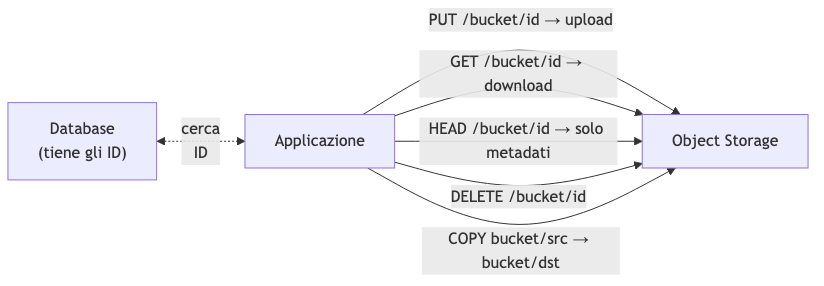
\includegraphics[keepaspectratio,alt={Diagramma Mermaid}]{images/mermaid-lezione-11-storage-architetture-e-servizi-05.png}}
\emph{Fig. --- Le operazioni fondamentali dell'object storage S3: PUT,
GET, HEAD, DELETE, COPY.}

\subsection{L'API S3}\label{lapi-s3}

L'API standard de facto dell'object storage è \textbf{S3} (\emph{Simple
Storage Service}), proposta e implementata da Amazon. Le operazioni core
sono:

\begin{itemize}
\tightlist
\item
  \textbf{PUT Object}: carica un oggetto in un bucket.
\item
  \textbf{GET Object}: scarica l'intero oggetto. Non esiste
  \texttt{seek}: non si può richiedere un range di byte interno senza
  scaricare tutto.
\item
  \textbf{DELETE Object}: elimina un oggetto.
\item
  \textbf{HEAD Object}: recupera solo i metadati senza scaricare il
  payload --- utile prima di decidere se scaricare un oggetto da
  gigabyte.
\item
  \textbf{COPY Object}: copia un oggetto internamente allo storage,
  operazione che il sistema esegue in modo ottimizzato senza richiedere
  download + upload.
\end{itemize}

\subsection{Scalabilità tramite Consistent
Hashing}\label{scalabilituxe0-tramite-consistent-hashing}

Il problema di un object storage distribuito su molti nodi è: dato un ID
oggetto, su quale server si trova? Mantenere un registro centralizzato
(database) creerebbe un bottleneck immediato.

La soluzione adottata da implementazioni come \textbf{RIAK} (citato dal
professore come esempio di object storage distribuito; l'attribuzione a
GitHub non è verificata --- RIAK è un key-value store distribuito di
Basho Technologies usato da vari provider, ma non risulta essere il
backend principale di GitHub) è il \textbf{consistent hashing}:

\pandocbounded{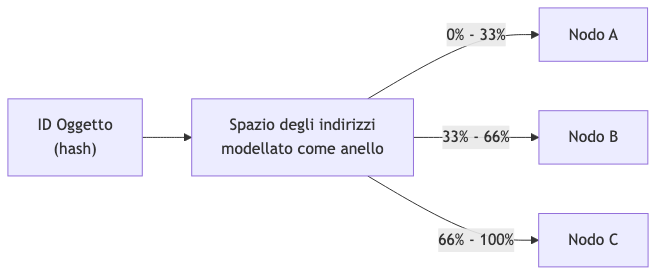
\includegraphics[keepaspectratio,alt={Diagramma Mermaid}]{images/mermaid-lezione-11-storage-architetture-e-servizi-06.png}}
\emph{Fig. --- Consistent hashing: l'ID dell'oggetto viene mappato
deterministicamente su un nodo senza consultare un registro
centralizzato.}

Lo spazio degli indirizzi viene trattato come un anello circolare e
diviso tra i nodi. Aggiungere un nodo richiede un algoritmo di
\textbf{ribilanciamento}, ma una volta completato ogni client può
determinare il nodo corretto direttamente dall'ID, senza interrogare
alcun registry.

\subsection{Vantaggi, limiti e casi
d'uso}\label{vantaggi-limiti-e-casi-duso}

{\def\LTcaptype{none} % do not increment counter
\begin{longtable}[]{@{}
  >{\raggedright\arraybackslash}p{(\linewidth - 6\tabcolsep) * \real{0.2500}}
  >{\raggedright\arraybackslash}p{(\linewidth - 6\tabcolsep) * \real{0.2500}}
  >{\raggedright\arraybackslash}p{(\linewidth - 6\tabcolsep) * \real{0.2500}}
  >{\raggedright\arraybackslash}p{(\linewidth - 6\tabcolsep) * \real{0.2500}}@{}}
\toprule\noalign{}
\begin{minipage}[b]{\linewidth}\raggedright
Caratteristica
\end{minipage} & \begin{minipage}[b]{\linewidth}\raggedright
Object Storage
\end{minipage} & \begin{minipage}[b]{\linewidth}\raggedright
NAS
\end{minipage} & \begin{minipage}[b]{\linewidth}\raggedright
SAN
\end{minipage} \\
\midrule\noalign{}
\endhead
\bottomrule\noalign{}
\endlastfoot
Accesso & HTTP REST & NFS / SMB & Fiber Channel / iSCSI \\
Struttura & Flat (bucket) & Gerarchica (cartelle) & Blocchi grezzi \\
Scalabilità & Massiva (exabyte+) & Media & Media \\
Latenza & Alta (HTTP overhead) & Media & Bassa \\
Memory Mapping & No & No & Sì \\
Casi d'uso & Backup, media, IoT, ML datasets & Document share & VM disk,
database \\
\end{longtable}
}

L'object storage è la soluzione ideale per \textbf{healthcare}
(archiviazione di scan e immagini diagnostiche: si scrive una volta, si
rilegge integralmente, non si modifica), \textbf{media storage},
\textbf{backup}, e qualsiasi scenario con \textbf{scrittura massiva e
lettura infrequente}.

\begin{calloutnote}{File system sull’object storage}

È possibile costruire un file system sopra l'object storage: gli oggetti
diventano blocchi, e la struttura gerarchica viene implementata a
livello applicativo. Questo permette di scalare fino a miliardi di
oggetti, ma le prestazioni non sono paragonabili a un file system nativo
su SAN.

\end{calloutnote}

\begin{center}\rule{0.5\linewidth}{0.5pt}\end{center}

\section{HCI --- Hyperconverged
Infrastructure}\label{hci-hyperconverged-infrastructure}

\subsection{Il problema con SAN e SSD ad alte
prestazioni}\label{il-problema-con-san-e-ssd-ad-alte-prestazioni}

Circa tredici anni fa, mentre la virtualizzazione VMware era al suo
apice, si osservò un problema strutturale nella SAN classica: la
topologia \emph{a stella} (tutti i server connessi a un controller
centrale) soffre di un collo di bottiglia fisico nel controller stesso.
Con un solo head node da 8 porte da 400 Gbit/s, si ottengono al massimo
3.2 Tbit/s aggregati --- e quando decine di SSD veloci sono dall'altro
lato, quella capacità finisce subito.

La startup \textbf{Nutanix} propose un approccio radicalmente diverso.

\subsection{Il paradigma HCI}\label{il-paradigma-hci}

L'idea centrale è \textbf{trasporre la matrice}: invece di separare
compute, storage e network in strati orizzonali, si costruiscono
\textbf{nodi} che contengono un po' di tutto. Ogni nodo è un server
standard con CPU, RAM, dischi locali e schede di rete. Il software li fa
sembrare una SAN.

\pandocbounded{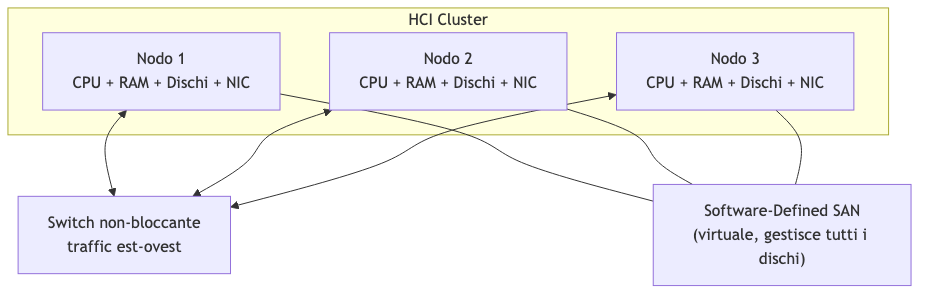
\includegraphics[keepaspectratio,alt={Diagramma Mermaid}]{images/mermaid-lezione-11-storage-architetture-e-servizi-07.png}}
\emph{Fig. --- HCI: i nodi collaborano via switch per formare una SAN
virtuale software-defined.}

Il \textbf{software HCI} (Nutanix AOS, VMware vSAN, Microsoft Storage
Spaces Direct) aggrega i dischi di tutti i nodi in un unico pool
storage, esponendolo come una SAN tradizionale alle virtual machine.

\subsection{Prestazioni: il vantaggio della
locality}\label{prestazioni-il-vantaggio-della-locality}

Il guadagno principale dell'HCI è la \textbf{data locality}: il software
può collocare il disco virtuale di una VM sullo stesso nodo fisico che
esegue quella VM. L'accesso va sul bus PCIe locale --- non attraversa
nessuna rete --- il che consente di sfruttare tutto il bandwidth di un
NVMe locale (decine di GB/s).

\begin{callouttip}{Traffico est-ovest}

In HCI la replica dei dati genera traffico \emph{est-ovest} (nodo →
nodo), non \emph{nord-sud} (server → controller centrale). Grazie agli
switch non-bloccanti dei datacenter moderni, questo traffico non
interferisce tra nodi diversi --- se N1 replica su N2, N3 non è
disturbato.

\end{callouttip}

\subsection{Resilienza: replication
factor}\label{resilienza-replication-factor}

Se un nodo cade, i dati che vi risiedevano non devono andare persi. La
soluzione è il \textbf{replication factor}:

\begin{itemize}
\tightlist
\item
  Con RF=2: ogni blocco scritto localmente viene replicato anche su un
  secondo nodo.
\item
  Con RF=3: replicato su altri due nodi (perdita di qualsiasi nodo è
  tollerata).
\end{itemize}

La scrittura funziona così: il nodo locale scrive sul proprio disco, poi
trasmette i dati al nodo remoto. Quando il nodo remoto conferma che i
dati sono in memoria (non necessariamente scritti su disco), il writer
viene sbloccato. Questo permette latenze di scrittura competitive con la
SAN.

\begin{calloutwarning}{Costi di licensing}

Tecnicamente, HCI è l'architettura con le migliori prestazioni assolute
oggi disponibile. Purtroppo, i vendor (Nutanix, VMware vSAN, Microsoft
Storage Spaces Direct) applicano licenze molto costose, che spesso fanno
riemergere la convenienza delle SAN tradizionali per molti contesti.

\end{calloutwarning}

\subsection{Scale-up vs Scale-out}\label{scale-up-vs-scale-out-1}

\begin{calloutdefinition}{Scale-up e Scale-out}

\textbf{Scale-up} (\emph{vertical scaling}): si aumenta la capacità di
un singolo nodo aggiungendo risorse (più RAM, più dischi). Limite
fisico: prima o poi il nodo non può crescere ulteriormente.

\textbf{Scale-out} (\emph{horizontal scaling}): si aggiungono nodi al
cluster. La capacità aggregata aumenta linearmente. HCI è
un'architettura scale-out.

\end{calloutdefinition}

Con HCI, aggiungere un nodo al cluster aumenta simultaneamente compute,
storage e network bandwidth in modo proporzionale e senza colli di
bottiglia centrali.

\begin{center}\rule{0.5\linewidth}{0.5pt}\end{center}

\section{Servizi Avanzati della SAN
Enterprise}\label{servizi-avanzati-della-san-enterprise}

Sia che si usi una SAN fisica tradizionale o un HCI software-defined, il
set di servizi gestiti è simile. Vediamoli nel dettaglio.

\subsection{Thin Provisioning}\label{thin-provisioning}

Quando si alloca una LUN da 2 TB a un utente, costui la percepisce come
un disco da 2 TB. Ma nella realtà, il sistema può \textbf{allocare
fisicamente solo una porzione} (es. 200 GB), espandendo lo spazio fisico
riservato man mano che il dato cresce.

\begin{callouttip}{Thin provisioning in pratica}

Il prof. Cisternino racconta di un progetto universitario per un
database di scan botanici. Stima iniziale: 75 TB. A distanza di dieci
anni, usano ancora meno di 10 TB. Grazie al thin provisioning, i
ricercatori hanno ricevuto 75 TB logici ma il sistema ha fisicamente
allocato solo lo spazio effettivamente usato, risparmiando decine di
migliaia di euro in storage.

\end{callouttip}

Il rischio è l'\textbf{overcommitment}: se si promettono 4 TB quando se
ne hanno 2 fisici e gli utenti li riempiono tutti, il sistema va in
crisi. È necessario monitorare l'utilizzo reale e agire prima che lo
spazio fisico finisca.

\begin{calloutnote}{Overcommitment reale}

Nel cluster HCI dell'Università di Pisa, 725 VM credono di avere 1.5 PB
di storage. Fisicamente il cluster ha circa 1 PB. Questo è un esempio
reale di thin provisioning e overcommitment in produzione.

\end{calloutnote}

\subsection{Multipath I/O}\label{multipath-io}

Il multipath connette un server allo storage tramite \textbf{più
percorsi paralleli} (più fibre ottiche, più HBA). I vantaggi sono:

\begin{itemize}
\tightlist
\item
  \textbf{Ridondanza}: se un percorso si guasta, il traffico viene
  automaticamente indirizzato sugli altri.
\item
  \textbf{Bandwidth aggregato}: i percorsi possono essere bilanciati per
  moltiplicare la banda disponibile.
\end{itemize}

Con gli SSD NVMe moderni da 16 GB/s ciascuno, il multipath è quasi
indispensabile: un singolo link da 100 Gbit/s (\textasciitilde12 GB/s)
non basta a saturare un solo SSD.

\subsection{Zoning e LUN Masking}\label{zoning-e-lun-masking}

Questi due meccanismi implementano il \textbf{controllo degli accessi} a
livello di storage:

\begin{itemize}
\tightlist
\item
  \textbf{Zoning}: definito nel fabric (switch Fiber Channel), determina
  quali server possono ``vedere'' quali parti dello storage. È una
  configurazione di rete: questo WWN (World Wide Name, l'identificatore
  del server) può comunicare con questo target.
\item
  \textbf{LUN Masking}: definito nel controller dello storage, determina
  quale LUN specifica è esposta a quale server. Anche se il server vede
  lo storage (per via dello zoning), potrebbe vedere solo alcune LUN.
\end{itemize}

\subsection{Snapshot, Clone e
Replicazione}\label{snapshot-clone-e-replicazione}

\textbf{Snapshot}: fotografia point-in-time di una LUN. Implementato
tipicamente con copy-on-write: la snapshot è inizialmente vuota e
registra solo i blocchi che cambiano dopo la sua creazione, occupando
pochissimo spazio inizialmente.

\textbf{Clone}: copia completa e indipendente di una LUN. Utile per
testare un aggiornamento critico: si clona la LUN di produzione, si
esegue l'aggiornamento sul clone, e se tutto funziona si promuove il
clone a produzione.

\textbf{Replicazione}: copia dei dati verso un secondo sito geografico.
Fondamentale per il \textbf{disaster recovery}. Esistono due modalità:

\begin{itemize}
\tightlist
\item
  \textbf{Sincrona}: ogni scrittura è confermata solo quando è stata
  scritta su entrambi i siti. Nessuna perdita di dati, ma latenza
  aggiuntiva = limite di distanza.
\item
  \textbf{Asincrona}: le scritture vengono replicate con un certo
  ritardo. Nessun impatto sulle prestazioni, ma in caso di disastro si
  perde l'ultima finestra temporale.
\end{itemize}

\subsection{Metro Cluster}\label{metro-cluster}

Un \textbf{metro cluster} estende un cluster attivo-attivo tra
\textbf{due datacenter geograficamente vicini}. La soglia di circa
\textbf{300 km / \textless15 ms} citata dal professore è una linea guida
di vendor (Nutanix, VMware vSAN) per i loro algoritmi di clustering
sincrono, non un limite fisico: la latenza fisica su fibra a 300 km è
\textasciitilde3 ms round-trip, ma i protocolli applicano threshold più
conservativi. Gli algoritmi di clustering non si accorgono che i nodi
sono in edifici separati: vedono solo la latenza di rete aggiuntiva, che
rimane tollerabile.

\pandocbounded{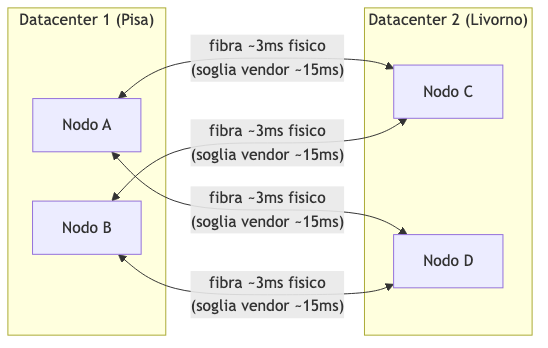
\includegraphics[keepaspectratio,alt={Diagramma Mermaid}]{images/mermaid-lezione-11-storage-architetture-e-servizi-08.png}}
\emph{Fig. --- Metro cluster: i nodi del cluster sono distribuiti su due
datacenter distinti ma vicini geograficamente.}

Oltre i 300 km (es. Milano-Napoli), la latenza supera la soglia
tollerabile per i protocolli sincroni. In quel caso si usa la
replicazione asincrona: si perde un po' di dati in caso di disastro, ma
almeno il sito remoto ha una copia recente.

\subsection{Tiering e Caching}\label{tiering-e-caching}

\textbf{Tiering}: lo storage viene diviso in livelli (\emph{tier}) con
caratteristiche diverse. I dati \emph{caldi} (frequentemente acceduti)
stanno su SSD, i dati \emph{freddi} (raramente acceduti) su HDD. Il
sistema \textbf{sposta automaticamente} i dati tra i tier in base ai
pattern di accesso (\emph{auto-tiering}).

\textbf{Caching}: i dati più caldi possono essere tenuti in \textbf{RAM}
del controller, eliminando completamente la latenza di accesso al disco
per le operazioni ripetute.

\pandocbounded{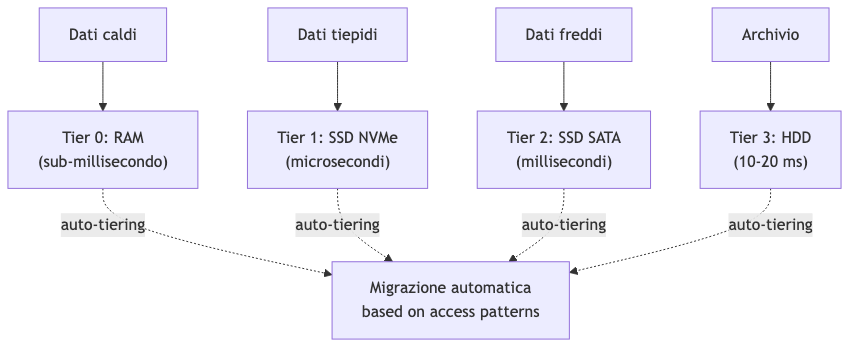
\includegraphics[keepaspectratio,alt={Diagramma Mermaid}]{images/mermaid-lezione-11-storage-architetture-e-servizi-09.png}}
\emph{Fig. --- Gerarchia di tiering: i dati migrano automaticamente
verso il tier più adatto in base alla frequenza di accesso.}

\subsection{Quality of Service (QoS)}\label{quality-of-service-qos}

La SAN può assegnare \textbf{priorità diverse} a LUN diverse: in un
momento di contesa, i blocchi della LUN A (database critico) vengono
serviti prima di quelli della LUN B (backup). Questo evita che un
processo I/O-intensivo (es. backup notturno) degradi le prestazioni di
un servizio di produzione.

\subsection{Sicurezza}\label{sicurezza-1}

\begin{itemize}
\tightlist
\item
  \textbf{Encryption at rest}: i dati vengono cifrati prima di essere
  scritti sui dischi. In memoria operativa sono in chiaro. Se un disco
  viene fisicamente sottratto, i dati sono illeggibili.
\item
  \textbf{Secure erase}: quando uno spazio viene liberato, i blocchi
  vengono sovrascritti per prevenire recupero non autorizzato di dati
  residui.
\item
  \textbf{Access control e autenticazione}: integrazione con sistemi di
  identità per controllare chi può accedere a quali LUN.
\item
  \textbf{Data integrity}: checksum dei blocchi per rilevare corruzioni
  silenti.
\end{itemize}

\begin{center}\rule{0.5\linewidth}{0.5pt}\end{center}

\section{Scelta dell'Architettura: non esiste ``la
migliore''}\label{scelta-dellarchitettura-non-esiste-la-migliore}

\begin{calloutwarning}{Non esiste un’architettura universalmente superiore}

SAN, NAS, Object Storage e HCI hanno ciascuno casi d'uso ottimali. La
scelta dipende sempre dal bilanciamento di performance, scalabilità,
costo e natura del workload.

\end{calloutwarning}

{\def\LTcaptype{none} % do not increment counter
\begin{longtable}[]{@{}
  >{\raggedright\arraybackslash}p{(\linewidth - 2\tabcolsep) * \real{0.5000}}
  >{\raggedright\arraybackslash}p{(\linewidth - 2\tabcolsep) * \real{0.5000}}@{}}
\toprule\noalign{}
\begin{minipage}[b]{\linewidth}\raggedright
Scenario
\end{minipage} & \begin{minipage}[b]{\linewidth}\raggedright
Architettura consigliata
\end{minipage} \\
\midrule\noalign{}
\endhead
\bottomrule\noalign{}
\endlastfoot
VM in produzione con accessi random intensi & SAN o HCI \\
Molte VM, budget limitato, buone prestazioni & HCI (se licensing
sostenibile) \\
Document store, backup, OneDrive aziendale & NAS \\
Archiviazione massiva (scan medici, dataset ML) & Object Storage (S3) \\
Big data, HPC, accessi paralleli & File system parallelo (Lustre,
GPFS) \\
Disaster recovery geograficamente distribuito & Replicazione asincrona
SAN \\
Ridondanza metropolitana (stesso provider) & Metro cluster \\
\end{longtable}
}

\begin{callouttip}{Dimensionamento: calcolo back-of-envelope}

Scenario: ingestire 1 TB/s di dati da sensori. - Un server con NIC da
100 Gbit/s = \textasciitilde12 GB/s di banda in ingresso. - Per
sostenere 1 TB/s: 1000/12 ≈ 84 server. - Con 100 server si ha margine
sufficiente. - I server processano localmente e inviano il risultato
alla SAN centrale. Non è necessario che tutta la banda in ingresso passi
per la SAN --- si fa buffer locale e trasferimento asincrono.

\end{callouttip}

\begin{center}\rule{0.5\linewidth}{0.5pt}\end{center}

\section{Caso Reale: il Cloud Privato dell'Università di
Pisa}\label{caso-reale-il-cloud-privato-delluniversituxe0-di-pisa}

Il prof. Cisternino ha mostrato l'infrastruttura reale del datacenter
UniPi come esempio concreto:

\begin{itemize}
\tightlist
\item
  \textbf{2 cluster HCI ibridi} (acquisiti \textasciitilde2019): storage
  con tier SSD + HDD, con auto-tiering automatico.
\item
  \textbf{1 cluster HCI all-flash} (più recente): tutto solid state, CPU
  più moderne, densità circa tre volte superiore rispetto ai cluster del
  2019 --- dimostrazione dell'andamento del costo dei dischi nel tempo.
\item
  \textbf{Server NAS per cold storage}: circa 1 petabyte di hard disk
  meccanici per archiviazione a lungo termine.
\item
  \textbf{Nessun Fiber Channel}: l'infrastruttura usa iSCSI su Ethernet
  ad alte prestazioni.
\end{itemize}

\begin{callouttip}{Overcommitment in produzione}

Il cluster HCI gestisce \textbf{725 virtual machine}. Le VM credono
collettivamente di avere \textbf{1.5 petabyte} di storage. Il cluster ha
fisicamente circa \textbf{1 petabyte}. Il thin provisioning permette
questo overcommitment perché la maggior parte delle VM non usa tutto lo
spazio che le è stato assegnato.

\end{callouttip}

\begin{center}\rule{0.5\linewidth}{0.5pt}\end{center}

\newpage

\chapter{Storage Avanzato e Introduzione al
Compute}\label{storage-avanzato-e-introduzione-al-compute}

La lezione riprende dal tema dello storage per completare alcuni
concetti rimasti aperti, introduce due nuove forme di storage emergenti
legate all'AI, approfondisce le metriche di performance e resilienza dei
dati, e apre il terzo grande pilastro del datacenter: il compute.

\begin{center}\rule{0.5\linewidth}{0.5pt}\end{center}

\section{Specializzazione hardware per
workload}\label{specializzazione-hardware-per-workload}

Prima del 2008 circa, il paradigma dominante era quello del server
generico: si comprava hardware e poi si decideva quale workload farci
girare. Questo approccio era sostenibile finché tutti i carichi di
lavoro erano sufficientemente simili. A partire dall'era della
virtualizzazione, e poi con il big data (intorno al 2013), ci si è resi
conto che \textbf{le prestazioni reali si ottengono solo specializzando
l'hardware al workload}.

Questa evoluzione vale per tutti i livelli dello stack: a livello di
storage, i vendor iniziarono a differenziare le proprie offerte per
workload specifici --- per il big data, ad esempio, i dischi SATA da
alta capacità diventarono preferibili ai dischi SAS più veloci ma
costosi, perché quel workload privilegia il rapporto capacità/prezzo
rispetto alla latenza unitaria. A livello di CPU, i produttori oggi
offrono configurazioni diverse dello stesso die, ottimizzate per
high-frequency single-thread oppure per il throughput parallelo massivo.

Questa specializzazione si riflette anche nelle architetture di storage:
SAN, NAS, HCI e object storage non sono intercambiabili, ma rispondono
in modo ottimale a classi di workload ben definite.

\begin{center}\rule{0.5\linewidth}{0.5pt}\end{center}

\section{Nuove forme di storage}\label{nuove-forme-di-storage}

\subsection{Stream-based storage}\label{stream-based-storage}

Il progetto \textbf{Nautilus} di Dell/EMC introdusse il concetto di
\emph{stream-based storage}: uno strato di persistenza pensato
specificamente per flussi di dati derivanti da sensori IoT. Un flusso
IoT è strutturalmente diverso da uno stream video: non trasmette
fotogrammi sequenziali di un'unica sorgente, ma campiona nel tempo lo
\textbf{stato del mondo} (temperatura, pressione, corrente) da molti
dispositivi in parallelo.

L'interesse computazionale di questo modello non è necessariamente
l'intera serie storica, ma spesso la misura corrente o aggregazioni su
finestre temporali. Il problema del \emph{store-and-forward}
tradizionale è che produce copie multiple dello stesso dato lungo la
catena di nodi, senza una politica chiara di ownership. Nautilus
risolveva questo garantendo che, in qualsiasi istante, ogni informazione
esistesse \textbf{in un'unica copia} nella rete di storage, con un
modello computazionale coerente sopra i flussi.

Il progetto non ha avuto un grande successo commerciale, ma l'ecosistema
open source ha risolto il problema in modo più pragmatico con framework
come \textbf{Apache Kafka} e simili. Il principio di base ---
\emph{store, process, forward} applicato a dati di serie temporali --- è
comunque centrale nella gestione di workload IoT e di edge computing.

\subsection{Vector database}\label{vector-database}

I \textbf{vector database} sono la forma di storage più rilevante emersa
negli ultimi anni, diretta conseguenza della diffusione dell'AI
generativa.

La ricerca testuale era già storicamente basata su vettori: dal modello
\emph{bag of words} degli anni '90, ogni documento veniva rappresentato
come un vettore nello spazio delle parole, con una dimensione per ogni
termine del vocabolario. La similarità tra un documento e una query si
calcolava con la \textbf{distanza coseno} tra i rispettivi vettori ---
base del funzionamento di motori di ricerca come Google. Il limite
fondamentale di questo approccio è la sua natura \emph{sintattica}: la
parola ``Python'' produce lo stesso vettore indipendentemente dal
contesto, rendendo impossibile distinguere il serpente dal linguaggio di
programmazione.

\begin{calloutdefinition}{Embedding}

Un \textbf{embedding} è un vettore denso ad alta dimensionalità prodotto
dalla prima parte di una rete neurale di un Large Language Model. A
differenza dei vettori bag-of-words (sparsi, binari), un embedding
cattura la \textbf{rappresentazione semantica} del testo nel suo
contesto. L'embedding di ``Python'' sarà diverso a seconda che la parola
appaia in un contesto di programmazione o zoologico, perché la rete ha
appreso la semantica durante il training.

\end{calloutdefinition}

OpenAI produce embedding di \textbf{3000 dimensioni} con valori
floating-point, uno spazio semantico molto ricco rispetto ai vettori
classici. Un risultato scientifico notevole (Cornell University) ha
dimostrato che esiste una \textbf{funzione di conversione} tra gli
embedding di modelli diversi: modelli addestrati su dati differenti
tendono a produrre rappresentazioni dello stesso significato che sono
mappabili l'una nell'altra, a meno di una trasformazione lineare. Questo
suggerisce l'esistenza di uno spazio latente universale del significato,
e giustifica l'investimento in architetture basate su embedding
indipendentemente dal modello specifico.

Un \textbf{vector database} combina la flessibilità dei database NoSQL
(collezioni di oggetti eterogenei, senza schema rigido) con la capacità
di indicizzare gli oggetti tramite i loro embedding e di rispondere a
query semantiche trovando i vettori più vicini nello spazio ad alta
dimensionalità.

\pandocbounded{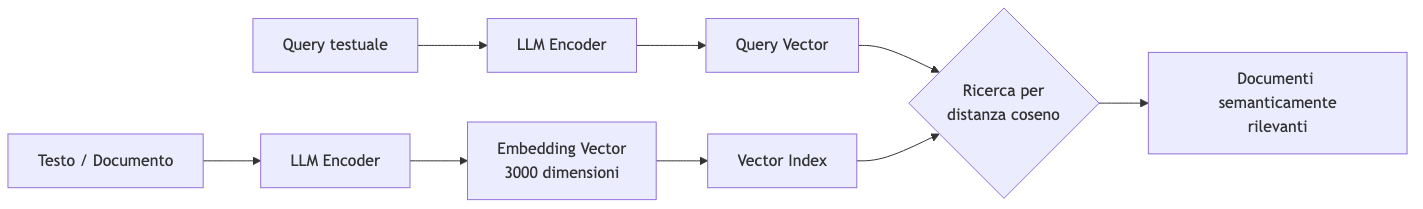
\includegraphics[keepaspectratio,alt={Diagramma Mermaid}]{images/mermaid-lezione-12-storage-avanzato-e-introduzione-al-compute-01.png}}
\emph{Fig. --- Pipeline di un vector database: i documenti vengono
indicizzati tramite embedding, e le query vengono risolte per similarità
semantica nello spazio vettoriale.}

\begin{callouttip}{RAG — Retrieval Augmented Generation}

La tecnica \textbf{RAG} (Retrieval Augmented Generation) è
l'architettura dominante dei sistemi AI moderni. Quando l'utente invia
un prompt, il sistema esegue prima una ricerca semantica su un database
di documenti (tramite vector search), inserisce i testi più rilevanti
nel contesto della richiesta, e solo poi il modello genera la risposta.
Questo riduce drasticamente le \emph{allucinazioni}: secondo lo Stanford
AI Index, anche i modelli migliori producono informazioni false nel 30\%
dei casi in modalità pura; il RAG riduce questo problema ancorando la
risposta a dati verificati.

\end{callouttip}

L'impatto sul datacenter è concreto: i sistemi di storage moderni (come
VAS DATA) stanno integrando capacità di esecuzione di reti neurali per
computare embedding direttamente durante l'ingestion dei dati. Lo
storage non è più solo un luogo dove i dati risiedono passivamente, ma
una componente attiva capace di costruire rappresentazioni semantiche e
rispondere a ricerche intelligenti.

\begin{center}\rule{0.5\linewidth}{0.5pt}\end{center}

\section{Misure di performance dello storage:
IOPS}\label{misure-di-performance-dello-storage-iops}

\textbf{Latenza} e \textbf{bandwidth} sono metriche insufficienti da
sole per caratterizzare le prestazioni di uno storage, perché dipendono
fortemente dal pattern di accesso.

\begin{calloutdefinition}{IOPS}

\textbf{IOPS} (Input/Output Operations Per Second) è il numero di
operazioni di I/O che uno storage riesce a completare in un secondo. Non
è una metrica assoluta: va sempre accompagnata dal tipo di accesso
(sequenziale o casuale), dalla dimensione del blocco, dal numero di
thread concorrenti e dal numero di code.

\end{calloutdefinition}

Il motivo della necessità di IOPS come metrica separata è intuitivo: uno
storage ottimizzato per leggere file video in streaming (dove
l'obiettivo è saturare la pipeline con dati contigui, con prefetching
aggressivo) si comporta in modo radicalmente diverso da uno storage che
serve il paging della memoria (accessi casuali a blocchi di 4 KB). Se si
misura solo la bandwidth in quest'ultimo caso, si ottiene un valore
molto inferiore rispetto a una lettura sequenziale dello stesso storage.

\begin{callouttip}{Analogia del supermercato}

\begin{itemize}
\tightlist
\item
  \textbf{IOPS} = clienti serviti al secondo
\item
  \textbf{Latenza} = tempo di servizio per cliente
\item
  \textbf{Code} = clienti in attesa
\item
  \textbf{Parallelismo} = numero di casse aperte
\end{itemize}

L'analogia spiega perché con una singola coda e un singolo cassiere, il
throughput è esattamente \texttt{1\ /\ latenza}. Con più casse in
parallelo, il throughput scala.

\end{callouttip}

La relazione matematica fondamentale con una singola coda è:

\[\text{IOPS} \approx \frac{1}{\text{latenza}}\]

Con più code o thread, il throughput scala proporzionalmente. Esempi
pratici: - HDD meccanico (latenza \textasciitilde5 ms):
\textasciitilde200 IOPS per coda - NVMe SSD (latenza \textasciitilde20
μs): \textasciitilde50.000 IOPS per coda

Lo storage è intrinsecamente asincrono: la CPU emette un'operazione di
lettura e viene sbloccata mentre l'operazione è in corso, permettendo
l'interleaving di più richieste da un singolo thread tramite code
multiple.

\begin{center}\rule{0.5\linewidth}{0.5pt}\end{center}

\section{Perdita di dati e
resilienza}\label{perdita-di-dati-e-resilienza}

\subsection{Tipologie di data loss}\label{tipologie-di-data-loss}

Concentrarsi solo sul guasto hardware come causa di perdita dati è un
errore comune. Le cause reali includono:

{\def\LTcaptype{none} % do not increment counter
\begin{longtable}[]{@{}
  >{\raggedright\arraybackslash}p{(\linewidth - 4\tabcolsep) * \real{0.3333}}
  >{\raggedright\arraybackslash}p{(\linewidth - 4\tabcolsep) * \real{0.3333}}
  >{\raggedright\arraybackslash}p{(\linewidth - 4\tabcolsep) * \real{0.3333}}@{}}
\toprule\noalign{}
\begin{minipage}[b]{\linewidth}\raggedright
Causa
\end{minipage} & \begin{minipage}[b]{\linewidth}\raggedright
Descrizione
\end{minipage} & \begin{minipage}[b]{\linewidth}\raggedright
Contromisura
\end{minipage} \\
\midrule\noalign{}
\endhead
\bottomrule\noalign{}
\endlastfoot
Guasto hardware & Disco rotto, controller danneggiato & RAID, replica \\
Corruzione software & Bug che sovrascrive dati validi & Checksum,
backup \\
Errore umano & File cancellati per sbaglio, misconfiguration & Backup,
snapshot \\
Ransomware/crittografia & Dati cifrati da malware & Backup offline,
snapshot \\
Perdita di chiavi crittografiche & BitLocker/encryption senza backup
della chiave & Key management \\
\end{longtable}
}

L'\textbf{errore umano} è statisticamente la prima causa di perdita
dati, largamente superiore a hardware e software combinati. Un sistema
di storage con replica perfetta non protegge da una cancellazione
accidentale: la cancellazione viene immediatamente replicata.

\subsection{Replica vs Backup}\label{replica-vs-backup}

La \textbf{replica} è una copia sincrona o asincrona dei dati su un
secondo storage, pensata per garantire disponibilità in caso di guasto
hardware. Il suo limite strutturale è che è una copia \emph{live} dello
stato corrente: qualsiasi corruzione o cancellazione si propaga
istantaneamente alla replica. La replica non protegge da errori logici.

Il \textbf{backup} è invece una copia \emph{puntuale nel tempo} dei
dati, conservata separatamente. Permette di ripristinare lo stato
precedente a un evento di corruzione o cancellazione. Il backup è
indispensabile indipendentemente dal livello di ridondanza dello
storage.

\subsection{Data breach secondo il
GDPR}\label{data-breach-secondo-il-gdpr}

\begin{calloutwarning}{Il GDPR definisce tre pilastri della sicurezza dei dati}

Un \textbf{data breach} non è solo la perdita di confidenzialità (dati
pubblicati o rubati). Il GDPR riconosce tre forme di violazione,
ciascuna con implicazioni legali: 1. \textbf{Confidenzialità}: dati
accessibili a soggetti non autorizzati 2. \textbf{Disponibilità}:
storage offline, dati irraggiungibili quando necessari 3.
\textbf{Integrità}: dati corrotti o modificati in modo non autorizzato

Un sistema che non può garantire la disponibilità dei propri dati è
soggetto a sanzioni esattamente come uno che subisce una fuga di
informazioni.

\end{calloutwarning}

\subsection{RPO e RTO}\label{rpo-e-rto}

\begin{calloutdefinition}{RPO — Recovery Point Objective}

L'\textbf{RPO} definisce la quantità massima di dati che si è disposti a
perdere in caso di failure, misurata in tempo. Un backup giornaliero
implica un RPO di 24 ore: in caso di incidente, si possono perdere fino
a un giorno di modifiche. L'RPO non può essere zero: se un software
malevolo corrompe i dati attivamente, anche i backup frequenti
conterranno dati corrotti a partire da un certo punto.

\end{calloutdefinition}

\begin{calloutdefinition}{RTO — Recovery Time Objective}

L'\textbf{RTO} definisce il tempo massimo tollerabile di downtime
durante un ripristino. Ripristinare un petabyte di dati può richiedere
più di un giorno anche con la migliore infrastruttura: questo deve
essere considerato nella progettazione del backup (più grande è il
backup unitario, maggiore è l'RTO).

\end{calloutdefinition}

La scelta dell'RPO è un bilanciamento economico: backup più frequenti
costano di più (bandwidth, storage, CPU). In certi casi il costo della
compliance supera il costo della sanzione, e l'organizzazione sceglie
consapevolmente di accettare un RPO meno stringente. Questa è una
decisione di risk management, non tecnica.

L'RPO e l'RTO si combinano con le politiche di replica: se si dispone
già di replica sincrona, il rischio residuo si riduce agli scenari in
cui entrambe le copie vengono perse simultaneamente, rendendo l'RPO
rilevante solo per quegli scenari estremi.

\subsection{Backup differenziale}\label{backup-differenziale}

Per gestire il costo del backup su dataset di grandi dimensioni, si usa
il \textbf{backup differenziale}:

\pandocbounded{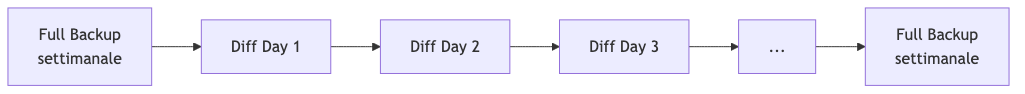
\includegraphics[keepaspectratio,alt={Diagramma Mermaid}]{images/mermaid-lezione-12-storage-avanzato-e-introduzione-al-compute-02.png}}
\emph{Fig. --- Schema di backup differenziale: un full backup periodico
viene completato da backup incrementali giornalieri che conservano solo
i blocchi modificati.}

Il ripristino richiede di applicare in sequenza il full backup e tutti i
diff successivi fino al punto desiderato, aumentando la complessità ma
riducendo drasticamente il volume di dati trasferiti.

\begin{center}\rule{0.5\linewidth}{0.5pt}\end{center}

\section{Snapshot dello storage}\label{snapshot-dello-storage}

Lo snapshot è una delle tecniche più potenti e versatili della gestione
dello storage.

\subsection{Meccanismo Copy-on-Write}\label{meccanismo-copy-on-write}

\begin{calloutdefinition}{Snapshot (Copy-on-Write)}

Uno \textbf{snapshot} è una fotografia logica dello stato di un volume
in un istante preciso, ottenuta senza copiare fisicamente i dati. Il
meccanismo utilizzato è il \textbf{Copy-on-Write (COW)}: al momento
dello snapshot, si registra semplicemente la mappatura corrente tra
blocchi logici e blocchi fisici. Quando una scrittura successiva
modifica un blocco, il nuovo dato viene scritto in un blocco fisico
\emph{nuovo}, mentre il blocco originale rimane intatto e viene
referenziato dallo snapshot.

\end{calloutdefinition}

Il funzionamento passo per passo:

\begin{enumerate}
\def\labelenumi{\arabic{enumi}.}
\tightlist
\item
  Volume logico: blocchi A, B, C, D → mappati ai blocchi fisici A, B, C,
  D
\item
  Si crea snapshot S1: S1 registra la mappatura A→A, B→B, C→C, D→D
\item
  Si modifica il blocco B: il nuovo contenuto viene scritto in B'
  (blocco fisico nuovo)
\item
  Il volume corrente punta a A, B', C, D; lo snapshot S1 punta ancora a
  A, B, C, D
\end{enumerate}

In questo modo, con un minimo overhead di metadati, si mantengono due
versioni logiche del volume condividendo i blocchi non modificati.

\begin{callouttip}{Casi d’uso pratici}

\begin{itemize}
\tightlist
\item
  \textbf{Aggiornamenti sicuri}: prima di un upgrade del database, si
  prende uno snapshot. Se l'upgrade fallisce, si ripristina
  istantaneamente lo stato precedente.
\item
  \textbf{Backup senza interruzione}: invece di fermare il database per
  fare il backup, si prende uno snapshot (operazione istantanea), e il
  sistema di backup copia i dati dallo snapshot mentre il database
  continua a operare.
\item
  \textbf{Test di aggiornamenti}: si crea un disco differenziale, si
  prova il cambiamento, e si scarta il diff se non soddisfacente.
\end{itemize}

\end{callouttip}

\begin{calloutwarning}{Effetto sullo spazio disponibile}

Con snapshot attivi, la dimensione logica del volume non riflette più lo
spazio fisico effettivamente disponibile: i blocchi referenziati dagli
snapshot non possono essere considerati liberi. Se il 75\% dei blocchi
viene riscrit\-to dopo uno snapshot, la dimensione fisica effettiva
diventa 1,75 volte quella logica. Per questo motivo è sconsigliato
mantenere snapshot per periodi prolungati, e lo storage può esaurirsi
inaspettatamente.

\end{calloutwarning}

\subsection{Esempi in sistemi reali}\label{esempi-in-sistemi-reali}

Il concetto di snapshot permea già i sistemi operativi comuni senza che
gli utenti ne siano consapevoli:

\begin{itemize}
\tightlist
\item
  \textbf{Windows Shadow Volume Copy (VSS)}: permette il backup di file
  in uso (normalmente bloccati da Windows) creando uno snapshot del
  volume, copiando dall'istantanea mentre l'applicazione continua a
  scrivere sulla copia live
\item
  \textbf{macOS Time Machine}: utilizza lo spazio libero del disco per
  mantenere snapshot automatici del filesystem, permettendo di ``tornare
  nel tempo'' a versioni precedenti dei file
\end{itemize}

\subsection{Backup application-consistent vs
crash-consistent}\label{backup-application-consistent-vs-crash-consistent}

Un backup può essere:

\begin{itemize}
\tightlist
\item
  \textbf{Crash-consistent}: si fotografa lo storage così com'è in un
  dato momento, senza sincronizzarsi con le applicazioni in esecuzione.
  I dati in memoria non ancora scritti su disco vengono persi. Al
  ripristino, il sistema si comporta come se avesse subito un crash
  improvviso, e le applicazioni applicano i loro meccanismi di recovery
  (WAL, journal). Accettabile per la maggior parte dei workload.
\item
  \textbf{Application-consistent}: l'applicazione (tipicamente un DBMS)
  viene notificata prima del backup, esegue un flush dei dati in-memory
  su disco, segnala allo storage di procedere con l'acquisizione in uno
  stato consistente. Garantisce una copia perfettamente integra al costo
  di maggiore complessità di coordinamento.
\end{itemize}

La strategia più comune è combinare i due approcci: crash-consistent per
le virtual machine generiche, application-consistent solo per i
database.

\begin{center}\rule{0.5\linewidth}{0.5pt}\end{center}

\section{Introduzione al Compute}\label{introduzione-al-compute}

La lezione introduce brevemente il terzo pilastro del datacenter, che
verrà approfondito nelle lezioni successive.

\subsection{La fine della scalabilità lineare del singolo
core}\label{la-fine-della-scalabilituxe0-lineare-del-singolo-core}

Per quasi 40 anni, la \textbf{Legge di Moore} ha garantito che il numero
di transistor raddoppiasse ogni due anni, producendo una progressione
esponenziale delle prestazioni computazionali. Questo ha reso possibile
l'AI moderna: i modelli neurali erano teoricamente noti dal 1989
(backpropagation), ma la quantità di dati e potenza computazionale
necessaria per addestrarli su scala era semplicemente indisponibile.

A un certo punto, la scalabilità del singolo core si è stabilizzata:
aumentare la frequenza di clock oltre certi limiti fisici diventa
impossibile. La risposta dell'industria è stata la
\textbf{replicazione}:

\pandocbounded{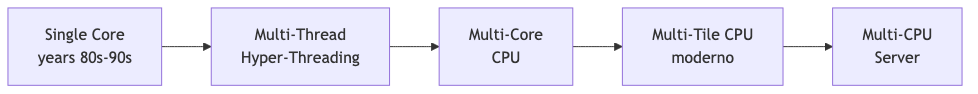
\includegraphics[keepaspectratio,alt={Diagramma Mermaid}]{images/mermaid-lezione-12-storage-avanzato-e-introduzione-al-compute-03.png}}
\emph{Fig. --- Evoluzione della gerarchia di replicazione
computazionale: ogni livello replica l'unità precedente per aumentare il
parallelismo gestendo la complessità a un livello di astrazione più
alto.}

Il concetto di \textbf{tile} è il più recente: un tile è un blocco di
core completo (con cache, controller, etc.) che può essere replicato sul
die come un componente standard, riducendo la complessità di
progettazione del fabric on-chip e permettendo configurazioni diverse
dello stesso prodotto semplicemente variando il numero di tile.

\subsection{Economia della produzione di
chip}\label{economia-della-produzione-di-chip}

La produzione di ASIC ha un'economia particolare: il costo fisso di
progettazione e realizzazione dei mask è elevatissimo (milioni di
dollari), e il software EDA per generare il layout dei transistor a
partire dal Verilog costa \textasciitilde\$1M/anno di licenze. Il punto
di breakeven si aggira sui 2 milioni di pezzi venduti. Questo spiega
perché solo pochissimi attori possono permettersi di produrre chip
custom, e perché i chip general-purpose come le CPU rimangono dominanti
nonostante l'efficienza degli ASIC dedicati.

\begin{calloutnote}{Prossime lezioni}

Il ciclo sul compute continuerà con: architetture CPU e GPU in
dettaglio, sistemi blade vs rack, formato OCP (Open Compute Project),
layout delle schede madri server, e il perché queste scelte
architetturali esistono.

\end{calloutnote}

\begin{center}\rule{0.5\linewidth}{0.5pt}\end{center}

\newpage

\chapter{Architettura Compute: CPU, GPU e
NPU}\label{architettura-compute-cpu-gpu-e-npu}

La lezione precedente aveva introdotto il tema del compute come terzo
pilastro del datacenter, partendo dall'evoluzione della Legge di Moore e
dalla necessità di replicare le unità computazionali in risposta ai
limiti fisici del singolo core. In questa lezione si approfondisce
l'architettura interna dei processori moderni --- CPU, GPU e NPU ---
analizzando le scelte di progetto che ne determinano le prestazioni. Si
introduce anche il contesto di sostenibilità energetica che vincola e
orienta queste scelte a livello infrastrutturale.

\begin{center}\rule{0.5\linewidth}{0.5pt}\end{center}

\section{Sostenibilità Energetica dei
Datacenter}\label{sostenibilituxe0-energetica-dei-datacenter}

\subsection{Il Report Annuale di Settore
2025}\label{il-report-annuale-di-settore-2025}

Uno dei temi di apertura della lezione riguarda il peso ambientale dei
datacenter. Il settore pubblica ogni anno report che misurano il consumo
energetico globale, l'impronta carbonica e l'utilizzo delle risorse
idriche. I dati 2025 confermano un trend preoccupante: il consumo
elettrico dei datacenter è in crescita esponenziale, trainato
principalmente dalla diffusione dell'AI generativa, che richiede cluster
di GPU sempre più grandi per l'addestramento e l'inferenza dei modelli.

Il consumo energetico va analizzato su due fronti distinti. Il primo è
il costo dell'elettricità in sé, che incide direttamente sulla
sostenibilità economica delle operazioni. Il secondo è
l'\textbf{impronta carbonica}: un datacenter alimentato da fonti
rinnovabili può avere lo stesso consumo in kWh di uno alimentato da
carbone, ma un impatto sul clima radicalmente diverso. I grandi cloud
provider comunicano i propri obiettivi di carbon neutrality, ma la
metrica rilevante non è il consumo lordo bensì il \textbf{carbon
intensity} dell'energia acquistata, che varia enormemente a seconda
della zona geografica e dell'ora del giorno.

\begin{calloutnote}{Power Usage Effectiveness (PUE)}

Il \textbf{PUE} (Power Usage Effectiveness) è il rapporto tra l'energia
totale consumata dal datacenter e quella assorbita dai soli apparati IT.
Un PUE di 1,0 è il valore ideale (tutta l'energia va ai server); i
datacenter moderni si attestano intorno a 1,2--1,4. I datacenter meno
efficienti superano 2,0, il che significa che per ogni watt di computing
si spreca più di un watt in overhead (soprattutto raffreddamento).

\end{calloutnote}

\subsection{Evaporazione dell'Acqua e
WUE}\label{evaporazione-dellacqua-e-wue}

Un tema emergente nei report 2025 riguarda il consumo idrico. I sistemi
di raffreddamento a torre evaporativa --- i più diffusi nei datacenter
di grandi dimensioni --- dissipano il calore attraverso
l'\textbf{evaporazione dell'acqua}: il calore viene trasferito
all'acqua, che evapora nell'atmosfera portando via l'energia termica.
Questo processo è efficiente dal punto di vista energetico (basso
consumo elettrico della torre) ma ha un costo idrico reale: un
datacenter di grandi dimensioni può consumare milioni di litri d'acqua
al giorno.

La metrica corrispondente è il \textbf{WUE} (Water Usage Effectiveness),
analogo al PUE per l'acqua: litri d'acqua consumati per kWh di energia
IT erogata. I report 2025 segnalano che, con il diffondersi di sistemi
di raffreddamento a liquido più efficienti (liquid cooling diretto sui
chip), il WUE sta migliorando nei nuovi datacenter, ma il parco
installato resta prevalentemente a raffreddamento evaporativo. La
tendenza è verso un bilanciamento tra PUE e WUE: ottimizzare solo il
consumo elettrico del raffreddamento può significare scaricare il costo
sull'acqua.

\begin{callouttip}{Sostenibilità come vincolo di progetto}

I grandi operatori di datacenter stanno incorporando PUE, WUE e carbon
intensity tra i criteri di selezione del sito e di progettazione
dell'impianto, non come requisiti facoltativi ma come vincoli
contrattuali verso i clienti enterprise che hanno propri obiettivi di
sostenibilità (scope 3 emissions).

\end{callouttip}

\begin{center}\rule{0.5\linewidth}{0.5pt}\end{center}

\section{Architettura della CPU
Moderna}\label{architettura-della-cpu-moderna}

\subsection{La Gerarchia di Cache}\label{la-gerarchia-di-cache}

Per comprendere l'architettura interna di una CPU moderna, il punto di
partenza è la \textbf{gerarchia di memoria}. L'accesso alla RAM
principale ha latenze dell'ordine dei 60--100 ns --- un'eternità per un
processore che completa operazioni ogni nanosecondo. La soluzione è una
cascata di cache on-chip, ognuna più lenta ma più grande della
precedente:

{\def\LTcaptype{none} % do not increment counter
\begin{longtable}[]{@{}llll@{}}
\toprule\noalign{}
Livello & Latenza tipica & Dimensione tipica & Condivisione \\
\midrule\noalign{}
\endhead
\bottomrule\noalign{}
\endlastfoot
Registro & \textless{} 1 ciclo & pochi byte & privato al core \\
L1 (dati + istruzioni) & \textasciitilde4 cicli & 32--64 KB & privato al
core \\
L2 & \textasciitilde12 cicli & 256 KB -- 1 MB & privato al core \\
L3 (LLC) & \textasciitilde40 cicli & 8--256 MB & condiviso tra core \\
RAM & \textasciitilde200 cicli & GB--TB & condivisa tra socket \\
\end{longtable}
}

La L3 è condivisa e rappresenta il principale punto di contesa tra i
core: ogni core che accede a dati non in L1/L2 deve attraversare
l'interconnessione intra-chip per raggiungere la L3 o la memoria.

\subsection{La Crossbar: Interconnessione
Intra-Chip}\label{la-crossbar-interconnessione-intra-chip}

Il problema dell'interconnessione tra core diventa critico quando si
scala a decine o centinaia di core sullo stesso die. L'approccio più
semplice --- un \textbf{bus condiviso} --- non scala: solo un master
alla volta può trasmettere, e con molti core il bus diventa
immediatamente un collo di bottiglia.

La soluzione adottata nelle CPU server moderne è la \textbf{crossbar} (o
\emph{crossbar switch}): un'interconnessione a matrice che permette
comunicazioni simultanee e indipendenti tra qualsiasi coppia
sorgente--destinazione. Concettualmente, è come un centralino
telefonico: più chiamate possono essere instradata contemporaneamente
purché non condividano né la sorgente né la destinazione.

\pandocbounded{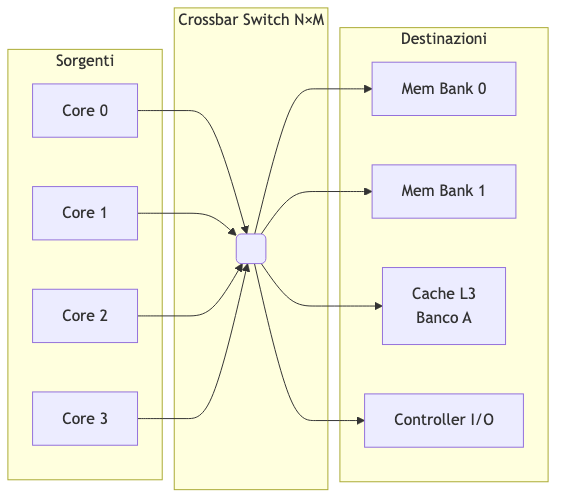
\includegraphics[keepaspectratio,alt={Diagramma Mermaid}]{images/mermaid-lezione-13-architettura-compute-cpu-gpu-e-npu-01.png}}
\emph{Fig. --- Schema di una crossbar N×M: ogni core può comunicare
simultaneamente con qualsiasi destinazione, senza contesa, purché le
coppie attive siano disgiunte.}

La crossbar garantisce \textbf{banda di bisection completa}: se ci sono
N sorgenti e M destinazioni, la crossbar ha N×M incroci, ognuno un
piccolo switch che viene attivato o meno. La complessità cresce come
O(N×M), il che diventa molto costoso in area di silicio per N e M
grandi. Per questo i progettisti di chip moderni spesso usano varianti
intermedie --- mesh 2D, ring bus, fabric gerarchici --- che offrono un
compromesso tra prestazioni e area occupata.

\begin{callouttip}{Infinity Fabric di AMD}

AMD EPYC utilizza l'\textbf{Infinity Fabric} come interconnessione
principale tra i die (chiplet) che compongono il processore. All'interno
di ogni chiplet il fabric ha caratteristiche di crossbar; tra chiplet
diversi opera come una rete a pacchetti ad alta velocità. Questo
permette di assemblare CPU con molti core replicando die più piccoli e
collaudabili, riducendo i costi di produzione.

\end{callouttip}

\subsection{Tile: Modularità del
Silicio}\label{tile-modularituxe0-del-silicio}

Il concetto di \textbf{tile} nasce dalla tendenza moderna a costruire
processori complessi non da un unico die monolitico, ma aggregando più
die specializzati tramite tecnologie di packaging avanzate. Ogni tile è
un'unità di silicio autonoma --- può contenere un gruppo di core, una
porzione di cache L3, un controller di memoria o un'interfaccia I/O ---
progettata e prodotta indipendentemente, poi interconnessa alle altre
tramite bus ad alta velocità integrati nel package.

Intel utilizza il termine \emph{tile} nell'architettura \textbf{Meteor
Lake} e nei processori Xeon \textbf{Sapphire Rapids}: il chip è composto
da una \emph{Compute Tile}, una \emph{GPU Tile}, una \emph{SoC Tile} e
una \emph{I/O Tile}, collegate tramite \textbf{EMIB} (\emph{Embedded
Multi-die Interconnect Bridge}) o \textbf{Foveros} (stacking 3D). AMD
usa il termine equivalente \emph{chiplet} per i die che compongono i
processori EPYC.

\begin{callouttip}{Vantaggi dell’approccio a tile}

Ogni tile può essere prodotta nel nodo tecnologico più adatto al suo
ruolo: la Compute Tile sul nodo più avanzato (dove il costo per
transistor è minimo), la I/O Tile su un nodo maturo ed economico (dove
la robustezza conta più della densità). Inoltre, un difetto di
fabbricazione colpisce una singola tile anziché l'intero die,
migliorando il \textbf{yield} --- la percentuale di chip funzionanti sul
totale prodotto --- e riducendo il costo medio del processore.

\end{callouttip}

\subsection{Hyperthreading e Multithreading
Simultaneo}\label{hyperthreading-e-multithreading-simultaneo}

L'\textbf{Hyperthreading} (HT) è il nome commerciale Intel per il
meccanismo architetturale noto come \textbf{SMT} (\emph{Simultaneous
Multithreading}). Il problema che risolve è l'idle time dei core: le
unità di esecuzione interne --- ALU, unità floating-point, unità di
load/store --- rimangono spesso inattive quando un thread è in stallo su
un cache miss o su una dipendenza tra istruzioni.

L'Hyperthreading aggira questo spreco duplicando le risorse
architetturali leggere --- il \textbf{register file} (i registri
visibili al software) e il \textbf{program counter} --- mantenendo
invece condivise le unità di esecuzione fisiche. Il risultato è che il
sistema operativo vede \textbf{due core logici} per ogni core fisico e
può schedulare due thread indipendenti: quando il primo è in stallo, il
core esegue istruzioni del secondo, riducendo l'idle time complessivo.
Il guadagno effettivo dipende fortemente dal workload: carichi con
frequenti accessi a memoria beneficiano maggiormente; carichi
computazionalmente densi e cache-friendly vedono vantaggi ridotti,
poiché i due thread si contendono le stesse unità di esecuzione.

\begin{calloutwarning}{Hyperthreading e vulnerabilità side-channel}

La condivisione delle risorse fisiche tra due thread --- cache L1, TLB,
buffer di esecuzione --- è la stessa ragione per cui l'Hyperthreading
apre una superficie d'attacco per vulnerabilità side-channel come
\textbf{Spectre} e \textbf{MDS} (\emph{Microarchitectural Data
Sampling}). In questi attacchi, un thread malevolo osserva le variazioni
di timing nelle risorse condivise per inferire dati del thread vittima.
Alcune configurazioni di sicurezza ad alta sensibilità disabilitano HT
per eliminare completamente questa superficie.

\end{calloutwarning}

\begin{center}\rule{0.5\linewidth}{0.5pt}\end{center}

\section{NUMA --- Non-Uniform Memory
Access}\label{numa-non-uniform-memory-access}

\subsection{Il Problema dei Server
Multi-Socket}\label{il-problema-dei-server-multi-socket}

Nei server enterprise è comune installare due o quattro CPU fisiche
sullo stesso sistema, condividendo un unico spazio di indirizzamento
logico. Ogni socket (CPU fisica) dispone di canali di memoria dedicati a
cui è direttamente connesso. Quando un core appartenente al socket 0
accede a un dato che risiede nei moduli DIMM del socket 1, la richiesta
deve attraversare l'interconnessione inter-socket (Intel QPI/UPI, AMD
Infinity Fabric cross-die) --- un percorso fisicamente più lungo e con
latenza significativamente maggiore rispetto all'accesso locale.

\pandocbounded{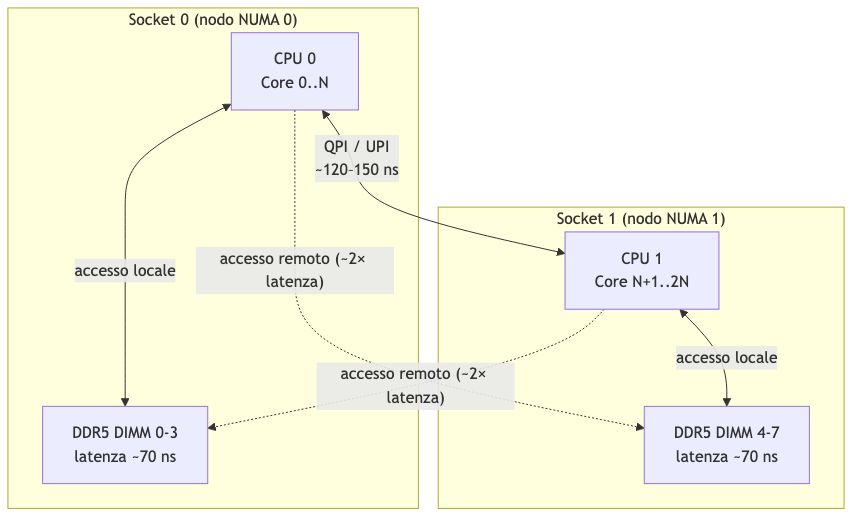
\includegraphics[keepaspectratio,alt={Diagramma Mermaid}]{images/mermaid-lezione-13-architettura-compute-cpu-gpu-e-npu-02.png}}
\emph{Fig. --- Architettura NUMA a due socket: l'accesso alla memoria
locale è circa 2× più rapido rispetto all'accesso alla memoria del
socket remoto.}

\begin{calloutdefinition}{NUMA — Non-Uniform Memory Access}

\textbf{NUMA} è un'architettura di memoria in cui la latenza di accesso
non è uniforme per tutti i processori: ogni CPU ha accesso preferenziale
(a bassa latenza) alla propria memoria locale, e accesso a latenza
maggiore alla memoria degli altri socket. Il sistema operativo gestisce
i nodi NUMA come entità distinte e cerca di allocare memoria nel nodo a
cui appartiene il thread che la utilizzerà.

\end{calloutdefinition}

\subsection{Implicazioni per il
Software}\label{implicazioni-per-il-software}

Un'applicazione ignara di NUMA può soffrire degradazioni di prestazioni
significative se i thread vengono schedulati su un socket mentre i dati
risiedono nell'altro. Il kernel Linux espone le topologie NUMA
attraverso il filesystem \texttt{/sys} e fornisce syscall
(\texttt{mbind}, \texttt{set\_mempolicy}) per il controllo esplicito
dell'allocazione. Database e middleware ad alte prestazioni (PostgreSQL,
Redis, DPDK) implementano politiche di affinità NUMA esplicita per
minimizzare la latenza degli accessi.

\begin{calloutwarning}{Virtualizzazione e NUMA}

Gli hypervisor devono propagare la topologia NUMA alle VM per permettere
al sistema operativo guest di ottimizzare. Se la VM è configurata con
vCPU e memoria che attraversano un confine NUMA fisico, le prestazioni
possono degradare silenziosamente senza un chiaro segnale di errore. I
tuner di VM enterprise (VMware, Hyper-V) hanno funzioni di NUMA spanning
che è importante configurare correttamente.

\end{calloutwarning}

\begin{center}\rule{0.5\linewidth}{0.5pt}\end{center}

\section{CPU vs GPU: Due Filosofie di
Calcolo}\label{cpu-vs-gpu-due-filosofie-di-calcolo}

\subsection{Il Diverso Obiettivo di
Progetto}\label{il-diverso-obiettivo-di-progetto}

La differenza fondamentale tra una CPU e una GPU non è di quantità ma di
filosofia: le due architetture rispondono a obiettivi di ottimizzazione
diametralmente opposti.

Una \textbf{CPU} è progettata per minimizzare la \textbf{latenza} della
singola operazione. Per raggiungere questo obiettivo, integra meccanismi
molto sofisticati: esecuzione fuori ordine (\emph{out-of-order
execution}), predizione dei branch, prefetching speculativo, pipeline
profonde e grandi cache private. Ogni core è in grado di eseguire codice
arbitrariamente complesso nel minor tempo possibile, gestendo dipendenze
tra istruzioni, salti condizionali imprevedibili e accessi a memoria non
sequenziali. Il prezzo di questa flessibilità è la dimensione: un core
CPU con tutta la sua logica occupa molto silicio.

Una \textbf{GPU} è progettata per massimizzare il \textbf{throughput} su
operazioni uniformi e parallele. I singoli core (chiamati \emph{shader
processor} o \emph{CUDA core}) sono molto più semplici --- pipeline
corte, nessuna predizione di branch, cache minima --- ma se ne integrano
migliaia sullo stesso die. Il modello di esecuzione è \textbf{SIMT}
(\emph{Single Instruction Multiple Threads}): un singolo flusso di
istruzione viene eseguito simultaneamente da centinaia di thread che
operano su dati diversi.

\pandocbounded{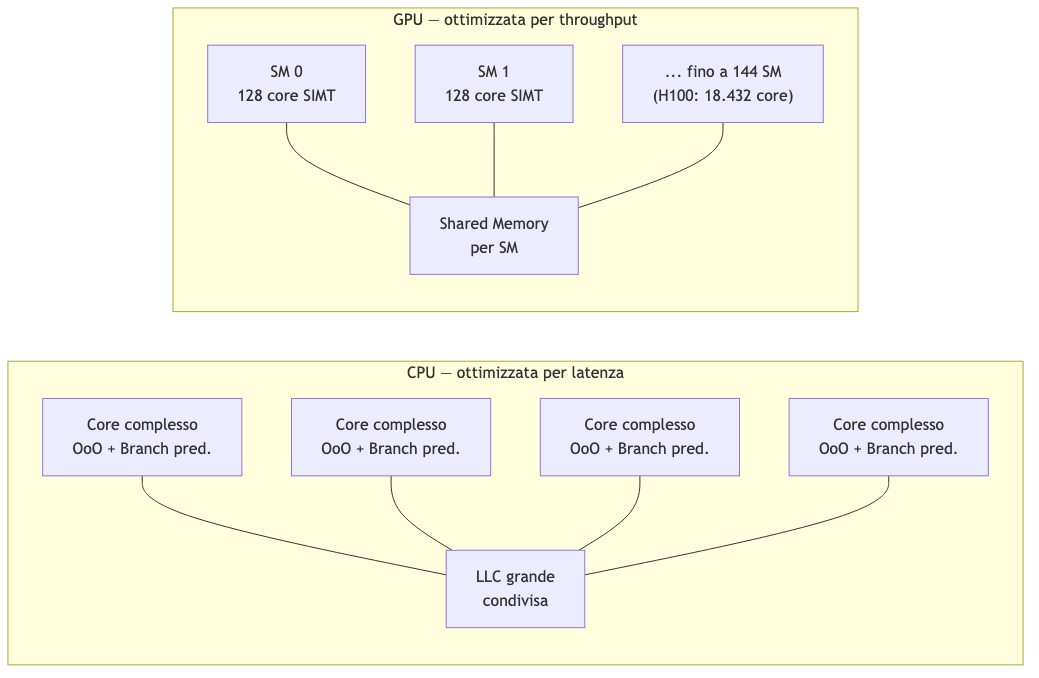
\includegraphics[keepaspectratio,alt={Diagramma Mermaid}]{images/mermaid-lezione-13-architettura-compute-cpu-gpu-e-npu-03.png}}
\emph{Fig. --- Confronto architetturale: la CPU dedica la maggior parte
del silicio alla logica di controllo (cache, predittori, scheduler OoO),
mentre la GPU lo dedica alle unità di esecuzione aritmetica in
parallelo.}

\subsection{Calcoli Vettoriali e SIMD}\label{calcoli-vettoriali-e-simd}

Il punto di forza della GPU è il calcolo vettoriale. Un'operazione come
la moltiplicazione matrice-vettore \(\mathbf{y} = \mathbf{A}\mathbf{x}\)
richiede di applicare la stessa operazione (prodotto scalare) a ogni
riga di \(\mathbf{A}\): sono migliaia di operazioni identiche su dati
diversi, esattamente il pattern che il modello SIMT della GPU esegue in
modo ottimale.

Le CPU moderne integrano anch'esse estensioni \textbf{SIMD}
(\emph{Single Instruction Multiple Data}) --- AVX-512 su x86 permette di
elaborare 16 float a 32 bit in parallelo con una singola istruzione ---
ma rimangono molto lontane dal parallelismo massivo di una GPU. La
differenza è di scala: 16 elementi in parallelo su CPU contro decine di
migliaia su GPU.

\begin{callouttip}{Perché l’AI ha bisogno della GPU}

Il training di un modello neurale consiste essenzialmente in milioni di
moltiplicazioni matriciali (forward pass + backpropagation). Queste
operazioni sono perfettamente adatte al modello SIMT della GPU: i dati
del mini-batch sono elaborati in parallelo da migliaia di core, e il
throughput scala quasi linearmente con il numero di core. Una GPU H100
di NVIDIA esegue circa 2.000 TFLOPS di operazioni fp8, circa 1.000× più
di una CPU di fascia alta.

\end{callouttip}

\begin{center}\rule{0.5\linewidth}{0.5pt}\end{center}

\section{NPU --- Neural Processing
Unit}\label{npu-neural-processing-unit}

\subsection{Definizione e Motivazione}\label{definizione-e-motivazione}

Se la GPU è un acceleratore general-purpose per il calcolo parallelo, la
\textbf{NPU} (\emph{Neural Processing Unit}) è un acceleratore
specializzato esclusivamente per le operazioni delle reti neurali --- in
particolare la moltiplicazione di matrici a bassa precisione numerica e
le operazioni di attivazione.

\begin{calloutdefinition}{NPU — Neural Processing Unit}

Una \textbf{NPU} è un circuito integrato (o un blocco IP all'interno di
un SoC) progettato specificamente per eseguire inferenza di reti neurali
con la massima efficienza energetica possibile. A differenza della GPU,
che è flessibile ma relativamente energivora, la NPU è ottimizzata per
un insieme ristretto di operazioni eseguite su dati a bassa precisione
(INT8, INT4, FP8), raggiungendo prestazioni per watt molto superiori.

\end{calloutdefinition}

L'operazione dominante nelle reti neurali trasformer è la
moltiplicazione tra matrici dense (\emph{GEMM --- General Matrix
Multiply}). Una NPU integra tipicamente un grande array di
moltiplicatori-accumulatori (\textbf{MAC} --- Multiply-Accumulate)
organizzato in una struttura \textbf{systolic array}: i dati scorrono
attraverso la griglia di MAC senza tornare in memoria centrale ad ogni
operazione, riducendo drasticamente il collo di bottiglia della
bandwidth.

Le NPU sono ubique nei dispositivi edge moderni: il \textbf{Neural
Engine} dei chip Apple M e A-series, la \textbf{Hexagon NPU} di
Qualcomm, e il \textbf{Neural Processing Engine} di MediaTek sono tutti
esempi di NPU integrate in SoC per smartphone e laptop. Nei datacenter,
chip come il \textbf{Google TPU} (Tensor Processing Unit) applicano la
stessa filosofia a scala datacenter.

{\def\LTcaptype{none} % do not increment counter
\begin{longtable}[]{@{}
  >{\raggedright\arraybackslash}p{(\linewidth - 6\tabcolsep) * \real{0.2500}}
  >{\raggedright\arraybackslash}p{(\linewidth - 6\tabcolsep) * \real{0.2500}}
  >{\raggedright\arraybackslash}p{(\linewidth - 6\tabcolsep) * \real{0.2500}}
  >{\raggedright\arraybackslash}p{(\linewidth - 6\tabcolsep) * \real{0.2500}}@{}}
\toprule\noalign{}
\begin{minipage}[b]{\linewidth}\raggedright
\end{minipage} & \begin{minipage}[b]{\linewidth}\raggedright
CPU
\end{minipage} & \begin{minipage}[b]{\linewidth}\raggedright
GPU
\end{minipage} & \begin{minipage}[b]{\linewidth}\raggedright
NPU/TPU
\end{minipage} \\
\midrule\noalign{}
\endhead
\bottomrule\noalign{}
\endlastfoot
Flessibilità & Massima & Alta & Bassa (solo NN) \\
Efficienza energetica & Bassa & Media & Massima \\
Latenza inferenza & Alta & Media & Bassa \\
Costo & Medio & Alto & Medio \\
Uso tipico & Preprocessing, logica & Training, inferenza batch &
Inferenza edge/produzione \\
\end{longtable}
}

\subsection{Groq e l'LPU}\label{groq-e-llpu}

\textbf{Groq} è una startup fondata da ex ingegneri Google con
l'obiettivo di costruire un'architettura radicalmente diversa per
l'inferenza di modelli linguistici. Il loro prodotto principale è la
\textbf{LPU} (\emph{Language Processing Unit}), progettata
specificamente per l'inferenza di modelli transformer a bassa latenza.

La differenza architetturale principale rispetto a una GPU è
l'\textbf{esecuzione deterministica}: una GPU gestisce l'esecuzione dei
thread con scheduler hardware dinamici, e le prestazioni dipendono
dall'occupazione dei SM e dai pattern di accesso alla memoria. La LPU ha
invece un modello di esecuzione completamente statico --- il compilatore
Groq pianifica ogni operazione a compile time, eliminando qualsiasi
variabilità a runtime e i relativi overhead. Il risultato è un
throughput di token generati per secondo significativamente superiore
rispetto alle GPU per i modelli che entrano nella sua SRAM on-chip.

\begin{calloutnote}{Acquisizione da parte di NVIDIA}

Groq è stata acquisita da NVIDIA. L'acquisizione riflette l'interesse di
NVIDIA nel consolidare la propria posizione nel mercato dell'inferenza
AI, dove architetture alternative come la LPU rappresentavano una
potenziale alternativa competitiva per workload di inferenza
latency-sensitive.

\end{calloutnote}

\begin{center}\rule{0.5\linewidth}{0.5pt}\end{center}

\section{OCP --- Open Compute Project}\label{ocp-open-compute-project}

\subsection{Origini e Filosofia}\label{origini-e-filosofia}

Il \textbf{Open Compute Project (OCP)} è un'iniziativa di
standardizzazione hardware avviata da \textbf{Meta (Facebook)} nel 2011.
L'obiettivo originale era ambizioso: rendere open source le specifiche
dell'hardware datacenter --- server, alimentatori, rack, switch ---
nello stesso modo in cui il software open source aveva rivoluzionato lo
sviluppo applicativo.

Il contesto che ha motivato questa scelta è economico: i server
tradizionali di vendor come Dell, HP e Cisco incorporano margini elevati
e una serie di funzionalità (luci di stato, pannelli LCD, logiche di
gestione complesse) che hanno senso per un operatore generico ma che in
un datacenter hyperscaler --- dove migliaia di server sono monitorati
centralmente --- sono ridondanti e costose. Meta progettò i propri
server rimuovendo tutto ciò che non era necessario e pubblicando le
specifiche.

\begin{calloutdefinition}{Open Compute Project}

L'\textbf{OCP} è un consorzio no-profit che sviluppa e pubblica
specifiche hardware aperte per datacenter. I membri (Meta, Microsoft,
Google, Intel, AMD, e decine di produttori ODM) contribuiscono
specifiche e possono produrre hardware compatibile, riducendo il vendor
lock-in e incentivando la competizione sui costi. Le specifiche OCP
coprono server, rack, networking, storage e power.

\end{calloutdefinition}

\subsection{Impatto sull'Ecosistema
Datacenter}\label{impatto-sullecosistema-datacenter}

L'impatto dell'OCP è stato significativo su più livelli. A livello di
costi, i server OCP prodotti da ODM taiwanesi come Wiwynn, Quanta e
Foxconn costano tipicamente il 20--30\% in meno rispetto agli
equivalenti di brand. A livello di efficienza, le specifiche OCP
eliminano feature non necessarie e ottimizzano la gestione termica per
ambienti ad alta densità. A livello di standardizzazione, il rack OCP
19'' ha dimensioni standardizzate che permettono di mescolare componenti
di fornitori diversi.

\begin{calloutnote}{OCP e il datacenter tradizionale}

L'OCP non ha (ancora) sostituito il mercato dei server tradizionali. Le
sue specifiche sono adottate quasi esclusivamente dai grandi hyperscaler
e da operatori che possono gestire direttamente hardware senza livelli
di supporto intermediari. Un'azienda con un piccolo datacenter
on-premise preferirà tipicamente server con supporto vendor diretto e
garanzie contrattuali, dove il margine del produttore si traduce in un
servizio.

\end{calloutnote}

\begin{center}\rule{0.5\linewidth}{0.5pt}\end{center}

\section{Token Ring}\label{token-ring}

\subsection{Il Problema dell'Accesso al
Mezzo}\label{il-problema-dellaccesso-al-mezzo}

Il \textbf{Token Ring} è un protocollo di rete a livello data link (IEEE
802.5) sviluppato da IBM negli anni '80, che risolve il problema
dell'accesso condiviso al mezzo trasmissivo in modo radicalmente diverso
rispetto a Ethernet.

In Ethernet (CSMA/CD), ogni stazione ascolta il canale e trasmette
quando lo trova libero: in caso di collisione, entrambe le stazioni si
fermano e riprovano dopo un intervallo casuale. Questo approccio è
semplice ma non deterministico: in condizioni di carico elevato, il
numero di collisioni cresce e la latenza diventa imprevedibile.

Il Token Ring risolve questo problema con un meccanismo di
\textbf{controllo centralizzato del mezzo tramite token}: un frame
speciale chiamato \emph{token} circola continuamente lungo l'anello.
Solo la stazione che detiene il token ha il diritto di trasmettere. Dopo
la trasmissione, il token viene rilasciato e passa alla stazione
successiva.

\pandocbounded{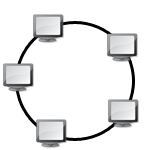
\includegraphics[keepaspectratio,alt={Topologia ad anello --- schema di una rete Token Ring}]{images/Ring-topology-22c5bb.png}}
\emph{Fonte: Wikimedia Commons --- Schema di topologia ad anello: ogni
nodo è connesso al precedente e al successivo, formando un percorso
chiuso per la circolazione del token.}

\pandocbounded{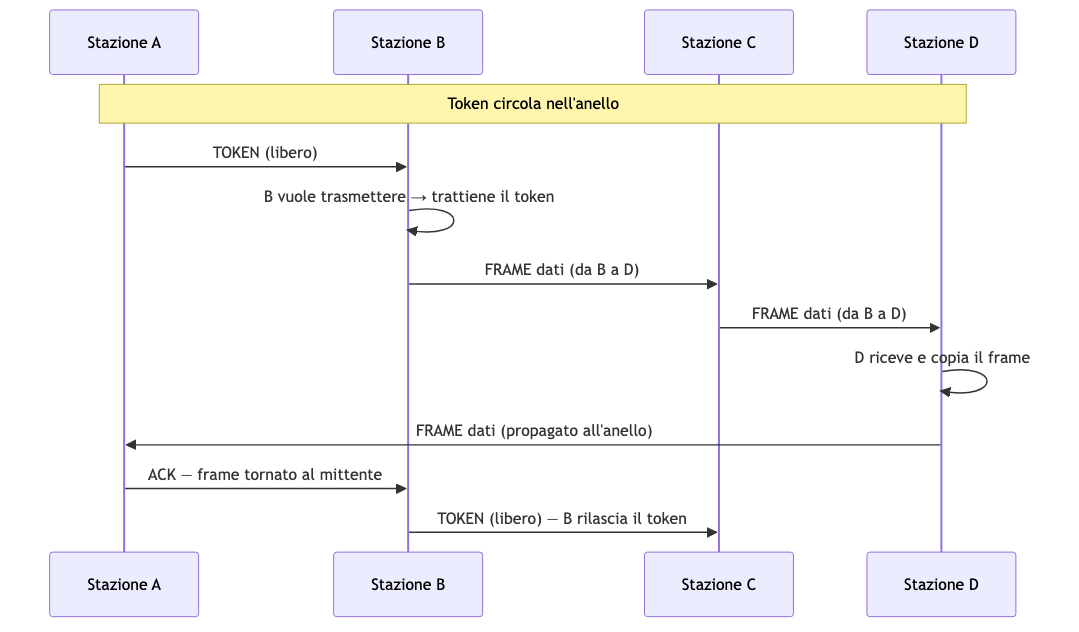
\includegraphics[keepaspectratio,alt={Diagramma Mermaid}]{images/mermaid-lezione-13-architettura-compute-cpu-gpu-e-npu-04.png}}
\emph{Fig. --- Circolazione del token e trasmissione di un frame in
Token Ring: il frame percorre l'intero anello e torna al mittente, che
lo rimuove e rilascia il token.}

\begin{callouttip}{Vantaggi del Token Ring rispetto a Ethernet}

Il Token Ring garantisce \textbf{accesso deterministico}: in un anello
con N stazioni, ogni stazione ottiene il token al massimo ogni N ×
\texttt{tempo\_di\_trasmissione\_massimo}. Questo lo rende adatto a
contesti industriali e real-time dove la latenza massima di accesso deve
essere garantita. Ethernet classica, essendo probabilistica, non offre
questa garanzia. Il prezzo è la complessità: gestire il token (elezione
del monitor, recupero del token perso) richiede protocolli aggiuntivi.

\end{callouttip}

Nonostante le sue proprietà eleganti, il Token Ring è stato soppiantato
da Ethernet per ragioni economiche: la semplicità e il costo inferiore
dell'hardware Ethernet, combinati con Ethernet switched (che elimina le
collisioni in modo diverso, mediante switch dedicati), hanno reso il
Token Ring commercialmente marginale dagli anni '90. Il concetto di
token, tuttavia, sopravvive in contesti diversi: le reti industriali
come \textbf{PROFIBUS} e alcune reti automotive usano meccanismi simili
per garantire latenze deterministiche.

\begin{center}\rule{0.5\linewidth}{0.5pt}\end{center}

\newpage

\chapter{Lezione 14 --- Server, BMC e
Containerizzazione}\label{lezione-14-server-bmc-e-containerizzazione}

\section{Server, BMC e
Containerizzazione}\label{server-bmc-e-containerizzazione}

Questa lezione chiude la parte hardware del corso e apre la parte
software. Si parte dall'anatomia fisica dei server rack, si analizza
come la crescente domanda di GPU ha trasformato radicalmente
l'architettura dei sistemi di calcolo, si introduce il \textbf{Base
Management Console (BMC)} come strumento fondamentale per la gestione
remota, e infine si affronta la \textbf{containerizzazione} --- la
tecnologia che disaccoppia il software dall'hardware fisico e che domina
il deployment moderno delle applicazioni.

\begin{center}\rule{0.5\linewidth}{0.5pt}\end{center}

\subsection{Architettura fisica dei
server}\label{architettura-fisica-dei-server}

\subsubsection{Il server rack 1U
standard}\label{il-server-rack-1u-standard}

Il punto di partenza è il server rack più diffuso: una macchina
\textbf{1U} (un'unità rack, circa 4,4 cm di altezza) ottimizzata per il
calcolo general purpose senza acceleratori GPU.

L'organizzazione interna segue un flusso d'aria da davanti a dietro e
riflette vincoli termici precisi:

\pandocbounded{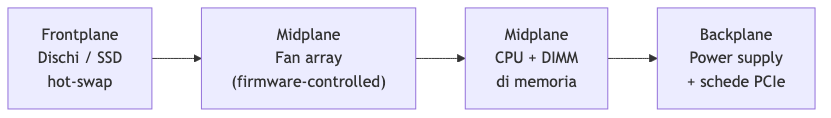
\includegraphics[keepaspectratio,alt={Diagramma Mermaid}]{images/mermaid-lezione-14-server-bmc-e-containerizzazione-01.png}}
\emph{Fig. --- Layout interno di un server 1U standard. L'aria entra dai
dischi anteriori e viene espulsa dal backplane.}

I \textbf{fan} non girano a velocità fissa: il firmware monitora
continuamente le temperature dei processori e aumenta o riduce la
velocità in modo proporzionale al carico computazionale. Un server idle
è quasi silenzioso; sotto carico pieno, il rumore è considerevole. Il
power supply tipico di un sistema 1U si attesta intorno ai \textbf{750
W}.

Questo tipo di server ha un numero massimo di socket CPU pari a due:
l'interconnessione tra più di due socket attraverso il bus esterno
diventa un collo di bottiglia significativo per la latenza e la banda di
memoria.

\subsubsection{Server four-way: scala
verticale}\label{server-four-way-scala-verticale}

Quando serve una grande quantità di RAM o si vogliono più socket CPU, si
ricorre a server da \textbf{4U o 5U} con architettura \textbf{four-way}
(quattro socket). Lo spazio aggiuntivo serve a:

\begin{itemize}
\tightlist
\item
  dissipatori più grandi per processori con TDP più elevato,
\item
  più slot DIMM per aumentare la memoria totale,
\item
  più bay per dischi,
\item
  più spazio per le schede PCIe.
\end{itemize}

Il four-way è la scelta giusta quando il collo di bottiglia è la
quantità di memoria: più socket significano più canali di memoria,
quindi più banda aggregata.

\subsubsection{Blade server: densità e semplificazione del
cabling}\label{blade-server-densituxe0-e-semplificazione-del-cabling}

\begin{calloutdefinition}{Blade Server}

Sistema modulare composto da uno \textbf{chassis condiviso} e da una
serie di schede di calcolo inseribili (le ``lame''), ciascuna delle
quali è un server autonomo. Lo chassis fornisce alimentazione
ridondante, fabric di rete integrato nel backplane e console di gestione
condivisa.

\end{calloutdefinition}

La storia del blade server è interessante. Alla fine degli anni '90, una
società britannica chiamata \textbf{RLX Technologies} (poi acquisita da
HP) aveva il problema di aumentare la densità di calcolo. L'idea fu
radicale: prendere la motherboard di un laptop, schiacciarla fino a
darle la forma di una scheda da inserire in uno chassis con guide. Tre o
quattro unità rack erano sufficienti a contenere \textbf{24 schede CPU},
creando una macchina parallela ad alta densità perfetta per applicazioni
come il web crawling dei motori di ricerca.

L'idea era così buona che fu adottata da tutti i principali vendor come
\textbf{form factor standard}. Il nome ``blade'' si riferisce proprio
alla forma allungata e sottile delle singole schede.

\pandocbounded{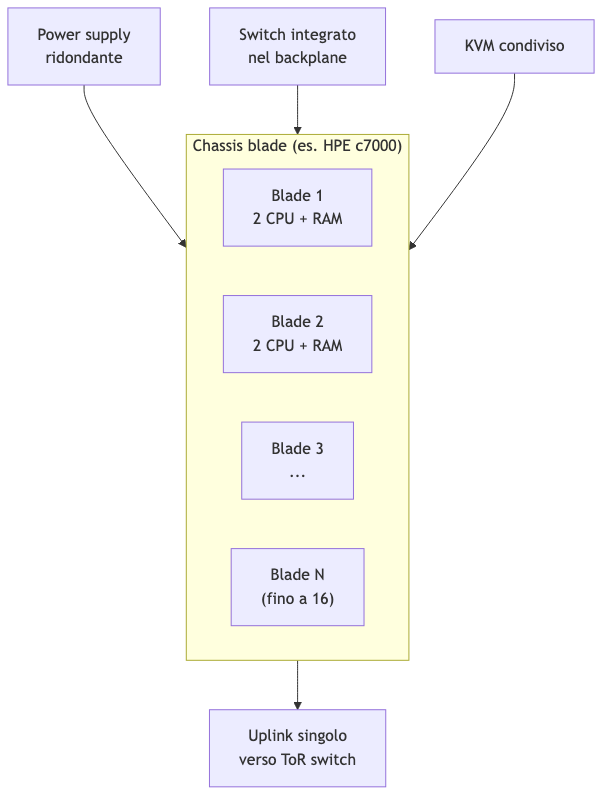
\includegraphics[keepaspectratio,alt={Diagramma Mermaid}]{images/mermaid-lezione-14-server-bmc-e-containerizzazione-02.png}}
\emph{Fig. --- Architettura di uno chassis blade. Lo switch nel
backplane connette tutte le lame; verso l'esterno esce un solo cavo
uplink per chassis.}

Il vantaggio principale del blade non è solo la densità CPU, ma la
\textbf{drastica semplificazione del cabling}: 16 nodi di calcolo
richiedono un solo cavo uplink verso il top-of-rack switch invece di 16
cavi separati. La gestione dell'infrastruttura diventa molto più
semplice.

Con un chassis HPE c7000 da 16 lame, ognuna con 2 CPU, si ottengono
\textbf{32 CPU in circa 10U}, ovvero circa \textbf{3.2 CPU/U} rispetto
alle \textbf{2 CPU/U} del server rack tradizionale.

\begin{calloutnote}{Blade e Ferrari F1}

Lo stesso chassis HPE BladeSystem c7000 mostrato a lezione era quello
utilizzato dalla scuderia Ferrari Formula 1 intorno al 2008 per le
simulazioni aerodinamiche.

\end{calloutnote}

\pandocbounded{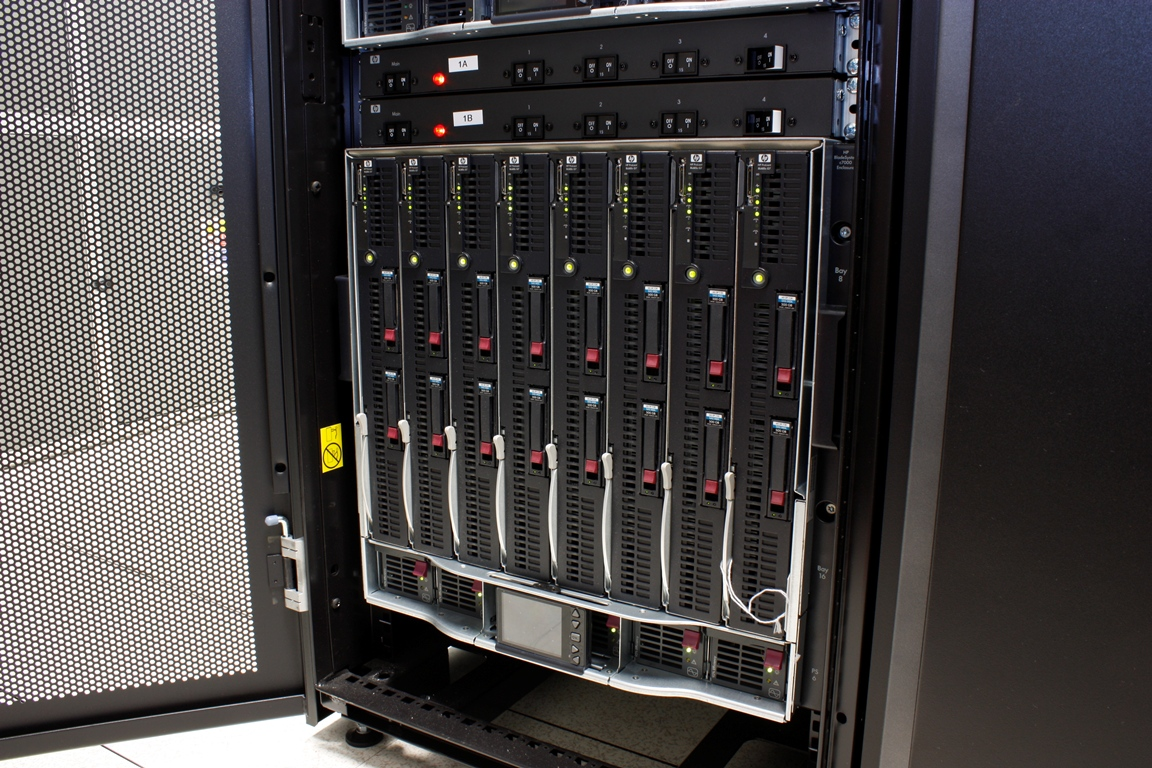
\includegraphics[keepaspectratio,alt={Chassis HPE BladeSystem c7000 con lame inserite}]{images/HP-BladeSystem-c7000-Enclosure-4a45b3.jpg}}
\emph{Fig. --- HPE BladeSystem c7000: uno degli chassis blade più
diffusi. Le lame si inseriscono frontalmente; il backplane ospita
switch, power supply e modulo KVM.}

Nel tempo, la crescita della banda di rete ha reso difficile scalare il
backplane dello chassis, e alcuni vendor hanno cercato di abbandonare il
formato. Il mercato ha però continuato a richiedere blade perché la
semplificazione del management è un valore reale. Oggi i blade esistono
ancora, affiancati da forme ibride.

\subsubsection{Twin architecture: densità senza networking
integrato}\label{twin-architecture-densituxe0-senza-networking-integrato}

\textbf{SuperMicro} ha introdotto circa 15 anni fa la \textbf{Twin
architecture} (o TwinPro): assomiglia superficialmente a un blade, ma lo
chassis condivide \textbf{solo l'alimentazione} --- non c'è networking
integrato nel backplane. Ogni nodo ha la propria scheda di rete
indipendente.

Il risultato è una densità ancora più elevata: \textbf{4 CPU/U} con nodi
disposti a coppie affiancate. Tecnicamente non è un blade, ma è spesso
classificato insieme a loro per la somiglianza visiva.

\subsubsection{Evoluzione dei server
GPU}\label{evoluzione-dei-server-gpu}

Prima dell'era AI, le GPU venivano inserite nei server come
\textbf{schede PCIe standard}, le stesse del gaming. La soluzione era
meccanicamente complicata: cavi di alimentazione supplementari,
strutture di supporto fragili, e la banda PCIe come bottleneck.

Con l'esplosione del machine learning, questa architettura non reggeva
più. NVIDIA ha risposto con \textbf{HGX}: le GPU non sono più schede
inseribili ma vengono \textbf{saldate direttamente sulla motherboard}
come se fossero CPU, collegate tra loro via \textbf{NVLink} che offre
una banda di circa \textbf{1 TB/s} --- ordini di grandezza superiori al
PCIe.

Il passo successivo è stato \textbf{Grace Hopper}: un modulo unico che
integra una CPU ARM (Grace) con una GPU H100 (Hopper) collegate tramite
NVLink-C2C ad altissima banda. Il risultato è che oggi la maggior parte
dei server AI viene \textbf{progettata direttamente da NVIDIA}, con HP,
Dell e altri che si limitano a ``mettere il box intorno''.

\pandocbounded{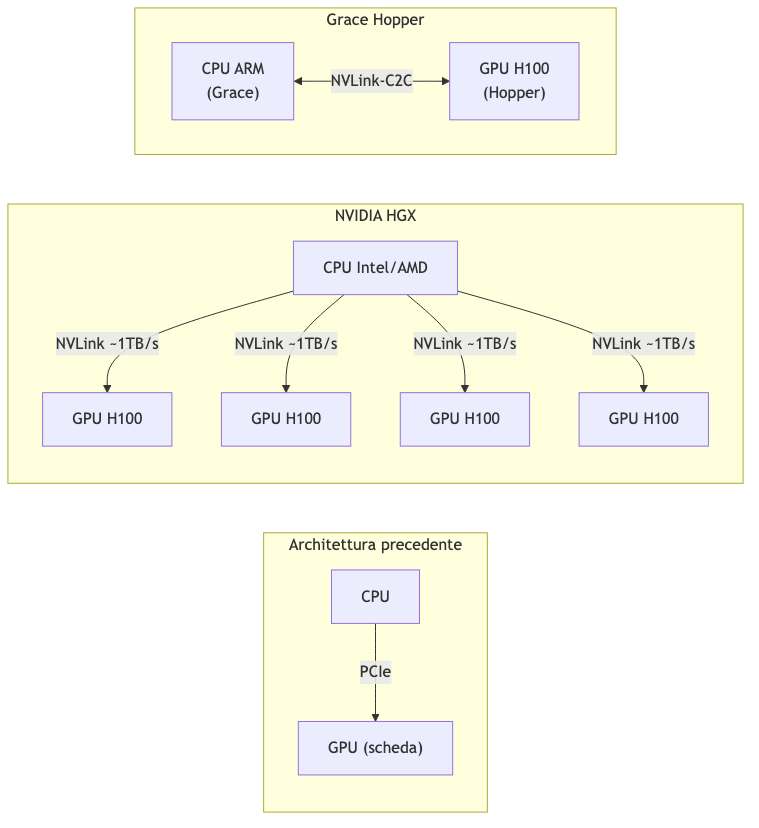
\includegraphics[keepaspectratio,alt={Diagramma Mermaid}]{images/mermaid-lezione-14-server-bmc-e-containerizzazione-03.png}}
\emph{Fig. --- Evoluzione dell'architettura GPU server: da scheda PCIe a
GPU on-board (HGX) fino al modulo integrato Grace Hopper.}

\begin{callouttip}{La proliferazione dei form factor come segnale}

Nel 2005 esistevano essenzialmente due form factor: 1U e 2U. Nel 2008 si
erano aggiunti i blade. Oggi esistono \textbf{decine} di form factor
diversi. Questa proliferazione non è casualità: è il segnale che il
calcolo general purpose è ormai inadeguato e che \textbf{l'hardware si
sta specializzando} per carichi di lavoro specifici. Ogni workload ha le
sue esigenze ottimali di densità GPU, RAM, storage e networking.

\end{callouttip}

\subsubsection{La filosofia del compromesso: server come
Lego}\label{la-filosofia-del-compromesso-server-come-lego}

Configurare un server è un esercizio di ottimizzazione vincolata: si
parte da uno spazio fisso (il rack unit) e si decide come riempirlo.

{\def\LTcaptype{none} % do not increment counter
\begin{longtable}[]{@{}ll@{}}
\toprule\noalign{}
Workload & Configurazione ottimale \\
\midrule\noalign{}
\endhead
\bottomrule\noalign{}
\endlastfoot
Calcolo intensivo (AI, HPC) & Poche drive, molte GPU, molto RAM GPU \\
Database in-memory & Server four-way, massima RAM CPU \\
Densità CPU pura, CPU-only & Twin o Blade \\
Calcolo GPU mid-range & Server 1U con schede PCIe RTX \\
\end{longtable}
}

Se si decide di mettere 24 drive in un server 2U, si rinuncia
necessariamente allo spazio per ulteriori schede PCIe o slot di memoria.
Ogni scelta di forma ha un costo in un'altra dimensione.

\begin{callouttip}{Risorse per esplorare form factor}

Il sito di \textbf{SuperMicro} è uno dei cataloghi più completi di form
factor server esistenti --- dalla singola scheda Twin al rack
pre-configurato con GPU. È un ottimo punto di riferimento per capire
concretamente la gamma di possibilità.

\end{callouttip}

\begin{center}\rule{0.5\linewidth}{0.5pt}\end{center}

\subsection{Base Management Console
(BMC)}\label{base-management-console-bmc}

\subsubsection{Il problema della gestione
remota}\label{il-problema-della-gestione-remota}

Un datacenter con centinaia o migliaia di server non può richiedere la
presenza fisica di un operatore per ogni operazione. Il \textbf{Base
Management Console (BMC)} risolve questo problema: è una scheda embedded
nel server con un proprio processore, memoria e sistema operativo,
completamente indipendente dallo stato del server principale.

\begin{calloutdefinition}{BMC — Base Management Console}

Componente hardware autonomo presente in ogni server enterprise che
fornisce accesso remoto completo alla macchina, indipendentemente dallo
stato del sistema operativo principale. Ogni vendor usa un nome
proprietario: \textbf{ILO} (HP), \textbf{iDRAC} (Dell), \textbf{IPMI} è
lo standard di protocollo sottostante.

\end{calloutdefinition}

\subsubsection{Funzionalità}\label{funzionalituxe0}

Il BMC espone un'interfaccia web raggiungibile tramite browser o SSH,
attraverso cui è possibile:

\begin{itemize}
\tightlist
\item
  \textbf{Monitorare} in tempo reale voltaggio, temperatura, velocità
  fan, watt consumati, stato di CPU e memoria,
\item
  \textbf{Accedere alla console virtuale}: una sessione che emula la
  connessione fisica monitor+tastiera, inclusa la possibilità di inviare
  Ctrl+Alt+Del (che nella tastiera PC è un interrupt hardware separato,
  non intercettabile dal sistema operativo),
\item
  \textbf{Montare immagini ISO} e installare un sistema operativo da
  remoto come se si inserisse un DVD fisico,
\item
  \textbf{Configurare BIOS e firmware} del server.
\end{itemize}

\pandocbounded{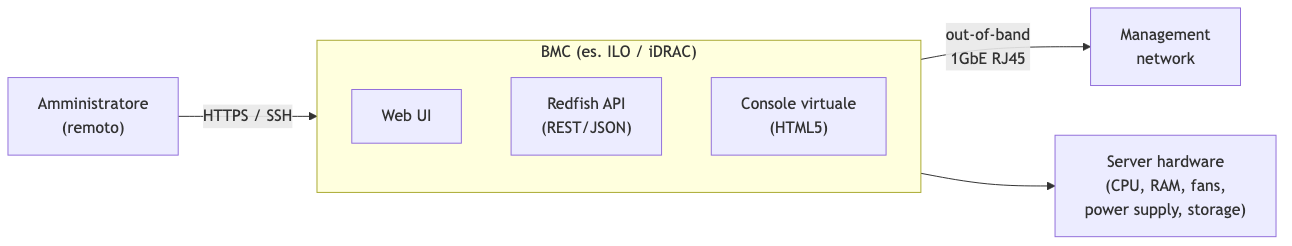
\includegraphics[keepaspectratio,alt={Diagramma Mermaid}]{images/mermaid-lezione-14-server-bmc-e-containerizzazione-04.png}}
\emph{Fig. --- Il BMC si connette alla management network tramite una
porta di rete dedicata e fornisce accesso completo all'hardware
indipendentemente dal sistema operativo.}

\subsubsection{Redfish API: automazione del
provisioning}\label{redfish-api-automazione-del-provisioning}

Per ambienti con molti server, la gestione manuale via web UI è
inefficiente. Lo standard \textbf{Redfish} definisce una API REST che
espone l'intero modello dati del server in JSON, permettendo
l'automazione completa:

\begin{verbatim}
GET  /redfish/v1/Systems/1                  # stato del sistema
POST /redfish/v1/Systems/1/Actions/
     ComputerSystem.Reset                   # reset del server
GET  /redfish/v1/Systems/1/Processors       # info CPU
GET  /redfish/v1/Chassis/1/Thermal          # temperature e fan
\end{verbatim}

Attraverso Redfish è possibile fare \textbf{zero-touch provisioning}:
uno script può formattare un server, montare un'immagine ISO, avviare
l'installazione e configurare il sistema --- tutto senza nessun
operatore fisicamente presente.

\subsubsection{Sicurezza della management
network}\label{sicurezza-della-management-network}

\begin{calloutwarning}{Il management network è equivalente all’accesso fisico}

Chiunque abbia accesso alla management network può riformattare
qualsiasi server, riavviarlo, modificarne il firmware, o estrarne le
credenziali. È un vettore di attacco \textbf{catastrofico} se esposto.

\end{calloutwarning}

Per questo motivo, il management network segue sempre uno di questi
modelli:

\begin{itemize}
\tightlist
\item
  \textbf{Rete fisicamente separata} dalla rete di produzione
  (out-of-band),
\item
  \textbf{VLAN dedicata} con accesso controllato da firewall/ACL,
\item
  Accesso esclusivamente tramite \textbf{VPN} con autenticazione forte.
\end{itemize}

La porta BMC è tipicamente una singola porta RJ45 da 1 GbE separata
dalle porte di dati. La sua separazione è un requisito architetturale,
non un'opzione.

\begin{center}\rule{0.5\linewidth}{0.5pt}\end{center}

\subsection{Containerizzazione}\label{containerizzazione}

\subsubsection{Il problema: accoppiamento tra software e
hardware}\label{il-problema-accoppiamento-tra-software-e-hardware}

Il datacenter fisico --- server, rete, storage, power, cooling --- è
l'infrastruttura. Sopra di essa vivono i \textbf{servizi}. Il problema
classico è che un servizio legato a un server fisico specifico si ferma
ogni volta che quel server deve essere manutenuto. Per costruire servizi
con alta disponibilità, occorre \textbf{disaccoppiare il software
dall'hardware sottostante}.

La virtualizzazione (macchine virtuali) risolve questo problema ma ha un
costo: ogni VM emula un hardware completo, ha il suo kernel, e occupa
risorse significative. I \textbf{container} offrono un compromesso
diverso: l'isolamento senza l'emulazione.

\subsubsection{CGroups: la primitiva del
kernel}\label{cgroups-la-primitiva-del-kernel}

La base tecnica dei container Linux è una funzionalità del kernel
chiamata \textbf{CGroups} (Control Groups), sviluppata originariamente
da Google.

\begin{calloutdefinition}{CGroups — Control Groups}

Feature del kernel Linux che introduce uno \textbf{scoping dei nomi} per
le risorse del sistema operativo. Invece di esporre globalmente tutti i
processi, file system, socket di rete e device, il kernel può
restringere la visibilità di un processo a un sottoinsieme di risorse
appartenenti allo stesso gruppo.

\end{calloutdefinition}

Il ragionamento è semplice. Normalmente, quando un processo chiede al
kernel ``dammi la lista dei processi in esecuzione'', riceve la lista
completa di tutti i processi del sistema. Con i CGroups, il kernel
risponde con la lista dei soli processi nello stesso container group.

La stessa logica si applica a: - \textbf{filesystem}: ogni container
vede solo il proprio albero di directory, - \textbf{networking}: ogni
container ha la propria interfaccia di rete virtuale, - \textbf{PID}: i
PID sono locali al container (il processo init dentro un container ha
PID 1), - \textbf{risorse CPU/memoria}: quote allocabili per container.

\begin{calloutnote}{Perché Google ha inventato i CGroups}

Google aveva bisogno di isolare ogni query di ricerca: se un utente
trovava il modo di far crashare il motore tramite una query malevola,
non doveva abbattere il servizio globale. Le VM erano troppo costose per
questo use case (una per ogni query). I CGroups permisero di creare un
container per ogni ricerca in modo quasi istantaneo, scaricarlo alla
fine, e garantire che nulla potesse ``uscire'' da quella query. Oggi
ogni ricerca Google gira in un container isolato.

\end{calloutnote}

\subsubsection{Differential file system: la base delle
immagini}\label{differential-file-system-la-base-delle-immagini}

Il secondo componente fondamentale è il \textbf{differential file
system} (o overlay filesystem). L'idea è analoga ai differenziali dei
dischi virtuali già visti nella parte di storage:

\pandocbounded{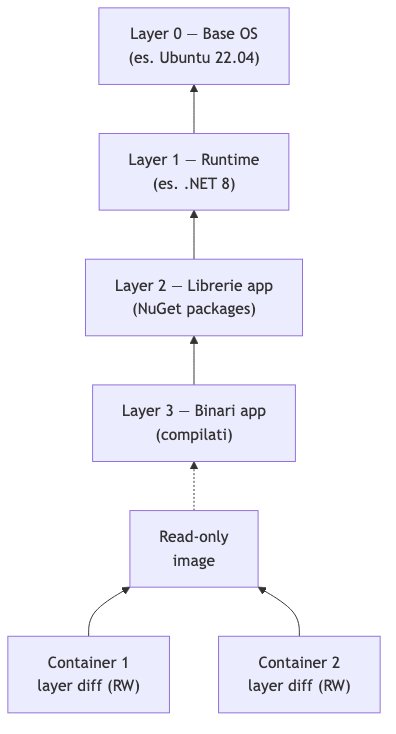
\includegraphics[keepaspectratio,alt={Diagramma Mermaid}]{images/mermaid-lezione-14-server-bmc-e-containerizzazione-05.png}}
\emph{Fig. --- Il differential file system permette a più container di
condividere gli stessi layer read-only. Solo le modifiche specifiche di
ogni container vengono scritte nel layer differenziale in cima.}

Dieci istanze dello stesso container condividono sul disco una sola
copia dei layer comuni. Solo le differenze generate a runtime --- file
di log, dati scritti, configurazioni modificate --- occupano spazio
aggiuntivo per ogni istanza.

\begin{calloutdefinition}{Container (definizione formale)}

Un container è un \textbf{insieme di processi} a cui il kernel Linux
fornisce una visione ristretta e isolata delle risorse di sistema,
grazie ai CGroups per il namespace isolation e a un differential
filesystem per l'isolamento del filesystem. Non include un kernel
proprio: condivide il kernel dell'host.

\end{calloutdefinition}

\subsubsection{Contenuto di un container vs macchina
virtuale}\label{contenuto-di-un-container-vs-macchina-virtuale}

\begin{calloutwarning}{Container ≠ Virtual Machine}

Un container condivide il kernel dell'host. Una VM ha il suo kernel
separato. Questa differenza è cruciale per la sicurezza:
\textbf{side-channel attacks} (Spectre, Meltdown, e varianti) che
sfruttano la condivisione della microarchitettura CPU sono possibili tra
container sullo stesso host, mentre sono molto più difficili tra VM. Il
container offre un isolamento logico, non un isolamento hardware.

\end{calloutwarning}

Poiché i container condividono il kernel, è possibile eseguire un
container \textbf{Debian su un host RedHat}: il kernel è lo stesso
(Linux), e la differenza tra le distribuzioni è essenzialmente nel
layout del filesystem e nelle versioni delle librerie dinamiche. Quando
un processo del container viene eseguito, il loader cerca le librerie
nel filesystem del container (Debian), non in quello dell'host.

Questo funziona perché il \textbf{kernel Linux API è straordinariamente
stabile}: le syscall non cambiano tra versioni. Il rischio esiste solo
se un container richiede funzionalità di un kernel molto più recente di
quello dell'host.

\pandocbounded{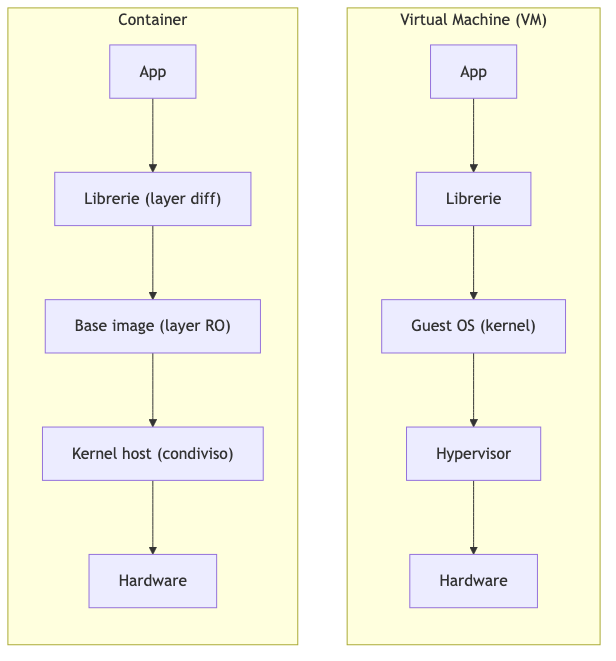
\includegraphics[keepaspectratio,alt={Diagramma Mermaid}]{images/mermaid-lezione-14-server-bmc-e-containerizzazione-06.png}}
\emph{Fig. --- Differenza strutturale tra VM e container. La VM porta il
proprio kernel; il container condivide quello dell'host.}

\subsubsection{Docker: la piattaforma container più
diffusa}\label{docker-la-piattaforma-container-piuxf9-diffusa}

\textbf{Docker} non è l'unico runtime container (esistono anche Podman,
containerd, LXC), ma è il più popolare e ha definito le convenzioni del
settore. Il file centrale è il \textbf{Dockerfile}: una sequenza
dichiarativa di istruzioni per costruire un'immagine.

\subsubsection{Multi-stage build: la pratica
comune}\label{multi-stage-build-la-pratica-comune}

Una caratteristica importante dei Dockerfile moderni è il
\textbf{multi-stage build}: si usano più immagini intermedie per
costruire l'applicazione, e si copia solo il risultato finale
nell'immagine di produzione.

\begin{verbatim}
## Stage 1: immagine di build (con compilatori e SDK)
FROM mcr.microsoft.com/dotnet/sdk:8.0 AS build
WORKDIR /src
COPY src/ src/
RUN dotnet restore
COPY . .
RUN dotnet build

## Stage 2: compilazione e publish
FROM build AS publish
RUN dotnet publish -o /app/publish

## Stage 3: immagine finale (solo runtime, senza compilatori)
FROM mcr.microsoft.com/dotnet/aspnet:8.0 AS final
WORKDIR /app
COPY --from=publish /app/publish .
EXPOSE 8080
ENTRYPOINT ["dotnet", "app.dll"]
\end{verbatim}

Il vantaggio di questo approccio è duplice: - \textbf{Sicurezza}:
l'immagine finale non contiene compilatori, SDK o tool di build. Un
attaccante che compromette il container non trova alcun compilatore C\#
disponibile, - \textbf{Dimensione}: l'immagine finale è molto più
piccola perché non include il layer con l'SDK.

Le istruzioni principali di un Dockerfile:

{\def\LTcaptype{none} % do not increment counter
\begin{longtable}[]{@{}
  >{\raggedright\arraybackslash}p{(\linewidth - 2\tabcolsep) * \real{0.5000}}
  >{\raggedright\arraybackslash}p{(\linewidth - 2\tabcolsep) * \real{0.5000}}@{}}
\toprule\noalign{}
\begin{minipage}[b]{\linewidth}\raggedright
Istruzione
\end{minipage} & \begin{minipage}[b]{\linewidth}\raggedright
Significato
\end{minipage} \\
\midrule\noalign{}
\endhead
\bottomrule\noalign{}
\endlastfoot
\texttt{FROM\ image\ AS\ name} & Base da cui si parte (o alias per
multi-stage) \\
\texttt{WORKDIR\ /path} & Imposta la directory di lavoro nel
container \\
\texttt{COPY\ src\ dst} & Copia file dall'host (o da un altro stage) nel
container \\
\texttt{RUN\ cmd} & Esegue un comando nel container durante la build \\
\texttt{ENV\ KEY=VALUE} & Definisce una variabile d'ambiente \\
\texttt{EXPOSE\ port} & Dichiara la porta che il container vuole
usare \\
\texttt{ENTRYPOINT\ {[}"cmd"{]}} & Processo principale avviato all'avvio
del container \\
\end{longtable}
}

\subsubsection{Port mapping e
networking}\label{port-mapping-e-networking}

Ogni container ha una propria interfaccia di rete virtuale. Se si vuole
rendere il container accessibile dall'esterno, occorre fare \textbf{port
mapping} (tecnicamente un NAT):

\begin{verbatim}
docker run -p 9000:8080 myapp   # porta host 9000 → porta container 8080
\end{verbatim}

Questo permette di avviare più istanze dello stesso container sullo
stesso host, ognuna con una porta esterna diversa, anche se tutte
internamente ascoltano sulla stessa porta 8080. Il meccanismo è
implementato tramite le regole \texttt{iptables} del kernel Linux.

\subsubsection{Docker Compose: composizione di
servizi}\label{docker-compose-composizione-di-servizi}

Un'applicazione reale raramente è un singolo processo. Una web app
tipica include: un \textbf{reverse proxy} (NGINX o Caddy), un
\textbf{application server} (il codice applicativo), e un
\textbf{database} (PostgreSQL, SQL Server). Docker Compose permette di
definire e avviare l'intero stack con un singolo file YAML:

\begin{Shaded}
\begin{Highlighting}[]
\FunctionTok{services}\KeywordTok{:}
\AttributeTok{  }\FunctionTok{frontend}\KeywordTok{:}
\AttributeTok{    }\FunctionTok{image}\KeywordTok{:}\AttributeTok{ nginx:alpine}
\AttributeTok{    }\FunctionTok{ports}\KeywordTok{:}\AttributeTok{ }\KeywordTok{[}\StringTok{"443:443"}\KeywordTok{,}\AttributeTok{ }\StringTok{"80:80"}\KeywordTok{]}
\AttributeTok{    }\FunctionTok{volumes}\KeywordTok{:}
\AttributeTok{      }\KeywordTok{{-}}\AttributeTok{ ./nginx.conf:/etc/nginx/conf.d/default.conf:ro}
\AttributeTok{    }\FunctionTok{depends\_on}\KeywordTok{:}\AttributeTok{ }\KeywordTok{[}\AttributeTok{app}\KeywordTok{]}
\AttributeTok{    }\FunctionTok{restart}\KeywordTok{:}\AttributeTok{ always}
\AttributeTok{    }\FunctionTok{networks}\KeywordTok{:}\AttributeTok{ }\KeywordTok{[}\AttributeTok{app{-}network}\KeywordTok{]}

\AttributeTok{  }\FunctionTok{app}\KeywordTok{:}
\AttributeTok{    }\FunctionTok{build}\KeywordTok{:}\AttributeTok{ .}
\AttributeTok{    }\FunctionTok{environment}\KeywordTok{:}
\AttributeTok{      }\KeywordTok{{-}}\AttributeTok{ ASPNETCORE\_ENVIRONMENT=Production}
\AttributeTok{      }\KeywordTok{{-}}\AttributeTok{ ConnectionStrings\_\_Default=Server=db;...}
\AttributeTok{    }\FunctionTok{ports}\KeywordTok{:}\AttributeTok{ }\KeywordTok{[}\StringTok{"8080:8080"}\KeywordTok{]}
\AttributeTok{    }\FunctionTok{depends\_on}\KeywordTok{:}\AttributeTok{ }\KeywordTok{[}\AttributeTok{db}\KeywordTok{]}
\AttributeTok{    }\FunctionTok{networks}\KeywordTok{:}\AttributeTok{ }\KeywordTok{[}\AttributeTok{app{-}network}\KeywordTok{]}

\AttributeTok{  }\FunctionTok{db}\KeywordTok{:}
\AttributeTok{    }\FunctionTok{image}\KeywordTok{:}\AttributeTok{ mcr.microsoft.com/mssql/server:2022{-}latest}
\AttributeTok{    }\FunctionTok{environment}\KeywordTok{:}
\AttributeTok{      }\KeywordTok{{-}}\AttributeTok{ SA\_PASSWORD=MySecurePass1!}
\AttributeTok{    }\FunctionTok{ports}\KeywordTok{:}\AttributeTok{ }\KeywordTok{[}\StringTok{"1433:1433"}\KeywordTok{]}
\AttributeTok{    }\FunctionTok{volumes}\KeywordTok{:}
\AttributeTok{      }\KeywordTok{{-}}\AttributeTok{ ./data:/var/opt/mssql}
\AttributeTok{    }\FunctionTok{networks}\KeywordTok{:}\AttributeTok{ }\KeywordTok{[}\AttributeTok{app{-}network}\KeywordTok{]}

\FunctionTok{networks}\KeywordTok{:}
\AttributeTok{  }\FunctionTok{app{-}network}\KeywordTok{:}
\AttributeTok{    }\FunctionTok{driver}\KeywordTok{:}\AttributeTok{ bridge}
\end{Highlighting}
\end{Shaded}

Quando si esegue \texttt{docker\ compose\ up}, Docker avvia tutti i
container definiti, crea la rete virtuale di tipo \textbf{bridge} che li
connette tra loro, e gestisce i volumi. I container si raggiungono per
nome (il container \texttt{app} può connettersi a \texttt{db} usando
\texttt{db} come hostname).

\begin{callouttip}{Perché le applicazioni container-native usano variabili d’ambiente}

Docker Compose permette di passare configurazioni ai processi tramite
variabili d'ambiente anziché file di configurazione. Questo è diventato
lo standard per le applicazioni moderne per due motivi: primo, è il
meccanismo naturale per iniettare configurazioni in un container senza
modificare l'immagine; secondo, le variabili d'ambiente sono intrinseche
al processo e non scritte su disco, quindi se il processo viene
terminato, la configurazione (incluse eventuali credenziali) scompare
con esso.

\end{callouttip}

\subsubsection{Container nel contesto AI e distribuzione
software}\label{container-nel-contesto-ai-e-distribuzione-software}

Il fenomeno si è espanso ben oltre le web app. \textbf{NVIDIA}
distribuisce i propri driver GPU per Linux esclusivamente come
container: la complessità dell'installazione (dipendenze, versioni del
kernel, moduli) era tale che impacchettarla in un container garantisce
che funzioni identicamente su qualsiasi host compatibile.

Più in generale, il container risolve il problema classico delle
dipendenze: se si usa Node.js, che può scaricare migliaia di pacchetti
durante \texttt{npm\ install}, basta fissare quei pacchetti nel
container al momento della build. L'applicazione gira sempre con le
stesse versioni, anche se il sistema ospite ha aggiornato le librerie.

\pandocbounded{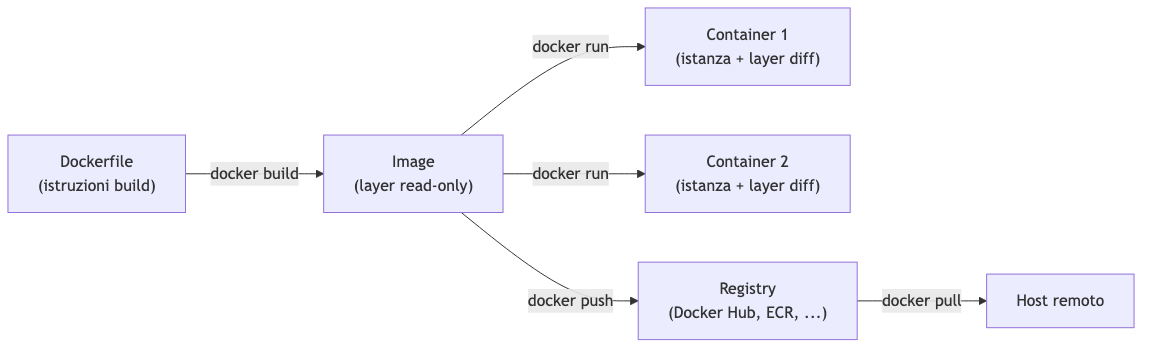
\includegraphics[keepaspectratio,alt={Diagramma Mermaid}]{images/mermaid-lezione-14-server-bmc-e-containerizzazione-07.png}}
\emph{Fig. --- Ciclo di vita di un container: dal Dockerfile
all'immagine, alle istanze in esecuzione, fino alla distribuzione
tramite registry.}

\begin{calloutnote}{Sintesi — Container}

Un container è un processo (o un gruppo di processi) a cui il kernel
Linux fornisce una visione isolata del sistema tramite \textbf{CGroups}
e un \textbf{differential filesystem}. Non include un kernel proprio.
Rispetto a una VM è molto più leggero (avvio in millisecondi, overhead
minimo), ma condivide il kernel con l'host, il che implica minore
isolamento di sicurezza. Docker è la piattaforma standard per costruire
(\texttt{Dockerfile}), distribuire (registry) e comporre
(\texttt{docker\ compose}) container. La tecnologia è stata inventata da
Google per isolare le query di ricerca ed è oggi il meccanismo di
deployment dominante nel software cloud-native.

\end{calloutnote}

\begin{center}\rule{0.5\linewidth}{0.5pt}\end{center}

\subsection{Prossimi argomenti}\label{prossimi-argomenti}

Il professore ha annunciato che le lezioni successive copriranno:

\begin{enumerate}
\def\labelenumi{\arabic{enumi}.}
\tightlist
\item
  \textbf{Virtualizzazione} --- il disaccoppiamento tra software e
  hardware tramite hypervisor, motivato dalla necessità di servizi
  sempre disponibili anche durante la manutenzione hardware,
\item
  \textbf{Cloud reference model} --- come il datacenter fisico diventa
  la base per i modelli di servizio cloud (IaaS, PaaS, SaaS).
\end{enumerate}

\newpage

\chapter{Virtualizzazione e
Containerizzazione}\label{virtualizzazione-e-containerizzazione}

La lezione affronta due tecnologie fondamentali per il datacenter
moderno: i \textbf{container} e le \textbf{macchine virtuali} (VM). Il
professore presenta intenzionalmente i container per primi, anche se
storicamente sono venuti dopo la virtualizzazione, perché permettono di
capire più facilmente il principio di isolamento. La virtualizzazione
vera e propria --- quella basata su hypervisor --- è invece la
tecnologia che ha reso possibile il cloud computing così come lo
conosciamo oggi.

\begin{center}\rule{0.5\linewidth}{0.5pt}\end{center}

\section{Container}\label{container}

\subsection{Il principio fondamentale: cgroups e
namespace}\label{il-principio-fondamentale-cgroups-e-namespace}

Un container non è un sistema operativo separato, ma una \emph{vista}
ristretta del sistema operativo esistente. Il meccanismo sottostante si
chiama \textbf{cgroup} (control group), un modulo del kernel Linux che
permette di raggruppare processi e limitare quali risorse di sistema
essi possono nominare.

\begin{callouttip}{Il potere del nome}

In informatica, nominare una risorsa è l'unica condizione necessaria per
potervi accedere. Un indirizzo di memoria è un nome. Un PID è un nome.
Se una risorsa non è nominabile --- cioè non è visibile nel namespace
del processo --- non esiste per quel processo. I cgroup sfruttano
proprio questo principio: mostrano ai processi del container solo le
risorse del proprio gruppo.

\end{callouttip}

Concretamente, quando un processo all'interno di un container esegue una
chiamata di sistema per elencare le risorse disponibili (altri processi,
interfacce di rete, filesystem), il kernel filtra la risposta mostrando
solo quelle appartenenti al suo cgroup. Il risultato è l'illusione di
avere un sistema operativo dedicato, pur condividendo lo stesso kernel
con tutti gli altri container sulla macchina.

Qui emerge la differenza fondamentale rispetto alle VM: \textbf{tutti i
container condividono lo stesso kernel}. Questo ha implicazioni di
sicurezza rilevanti: una vulnerabilità nel kernel colpisce
simultaneamente tutti i container in esecuzione. Un esempio recente e
concreto è \textbf{CVE-2026-31431 ``Copy Fail''}: un bug introdotto
nell'agosto 2017 nel modulo crittografico \texttt{authencesn} del kernel
Linux, rimasto silente per quasi dieci anni e scoperto nel 2026 grazie
ad analisi assistita da AI (strumento Xint Code). Un exploit di soli 732
byte di Python standard è sufficiente per ottenere privilegi di root su
tutte le principali distribuzioni Linux (Ubuntu, RHEL, Amazon Linux,
SUSE). Poiché il page cache del kernel è condiviso tra tutti i processi
--- inclusi quelli appartenenti a container diversi --- la vulnerabilità
non è solo una local privilege escalation ma anche un \textbf{container
escape} e un vettore di compromissione di nodi Kubernetes. Al momento
della lezione non esisteva una patch generale: la raccomandazione era
disabilitare il modulo se non strettamente necessario.

\subsection{Il filesystem
differenziale}\label{il-filesystem-differenziale}

Un container ha il proprio filesystem, ma questo non è una copia
completa: è un \textbf{filesystem differenziale} a strati (layer). Ogni
immagine container è definita da una sequenza di layer sovrapposti.
Quando si crea un container a partire da un'immagine base, si aggiunge
semplicemente un nuovo layer che registra solo le differenze rispetto a
quello precedente --- esattamente come un disco differenziale nelle VM.

\begin{callouttip}{Vantaggi del filesystem a layer}

Se dieci container derivano dalla stessa immagine base (ad esempio
Ubuntu), i layer comuni esistono una sola volta su disco. Al download,
se un layer è già presente localmente, non viene riscaricato. Questo si
traduce in risparmio di spazio e download incrementali.

\end{callouttip}

Il rovescio della medaglia è \textbf{prestazionale}: il filesystem
differenziale è una struttura dati complessa. Quando si accede a un
file, il sistema deve cercarlo nel layer corrente e, se non lo trova,
risalire ai layer precedenti. Più layer ci sono, più operazioni di I/O
sono necessarie. Per i dati che richiedono prestazioni elevate --- come
i file di un database --- è quindi consigliabile montare una directory
reale del filesystem host.

\subsection{Volumi e variabili
d'ambiente}\label{volumi-e-variabili-dambiente}

Due meccanismi permettono di iniettare configurazione e dati
dall'esterno nel container senza modificarne il filesystem interno:

\textbf{Variabili d'ambiente}: prima dell'era dei container erano
considerate un mezzo di configurazione obsoleto e scomodo. Docker le ha
riportate in auge perché rappresentano il modo più semplice per
iniettare parametri in un container senza dover accedere al suo
filesystem interno. La configurazione viene specificata al momento del
lancio del container e non richiede di modificare l'immagine.

\textbf{Volumi}: un volume è una directory (o file) del filesystem host
montata in una posizione specifica all'interno del container. Il
container la vede come parte del proprio filesystem, ma i dati risiedono
fisicamente sull'host. I casi d'uso principali sono: - Persistenza dei
dati oltre il ciclo di vita del container (es: directory dati di un
database) - Condivisione di dati tra più container - Iniezione di file
di configurazione o certificati senza ricostruire l'immagine

\begin{calloutwarning}{Dati persistenti nei container}

Se si esegue un database in un container senza montare un volume per la
directory dati, tutti i dati vengono persi quando il container viene
eliminato. Montare la directory \texttt{/var/lib/postgresql/data} (o
equivalente) su un volume host è pratica obbligatoria in produzione.

\end{calloutwarning}

\subsection{Rete nei container}\label{rete-nei-container}

Ogni container ha il proprio network namespace: il suo
\texttt{localhost} è diverso dal \texttt{localhost} dell'host e da
quello degli altri container. In Docker, ogni container riceve un
indirizzo IP nel range \texttt{172.x.x.x} della rete interna Docker. I
container non comunicano tra loro tramite \texttt{localhost}, ma tramite
questi indirizzi IP privati o tramite il nome del servizio definito in
Docker Compose.

Il mapping delle porte (\texttt{ports}) nel file di Compose permette di
esporre verso l'esterno una porta del container su una porta dell'host.
Poiché tutti i container condividono la stessa interfaccia di rete
fisica, non è possibile che due container siano in ascolto
contemporaneamente sulla porta 80 dell'host: il port mapping risolve il
conflitto assegnando porte diverse esternamente.

\begin{calloutnote}{Sicurezza della rete condivisa}

Nei container la scheda di rete fisica (\textbf{NIC}, \emph{Network
Interface Card}) dell'host è condivisa tra tutti i container in
esecuzione --- è lo stesso hardware che gestisce il traffico di tutti.
Nelle VM, invece, ogni macchina virtuale riceve una scheda di rete
virtuale dedicata (vNIC), emulata dall'hypervisor, con il proprio MAC
address e la propria identità di rete completa. Questa è una delle
differenze di isolamento più significative tra i due approcci.

\end{calloutnote}

\subsection{Docker Compose}\label{docker-compose}

Docker Compose permette di descrivere un'applicazione multi-container
come composizione di servizi in un file YAML. Il professore mostra un
esempio con tre servizi: un frontend (Nginx come reverse proxy), un
application server (backend su porta 8080) e un database (SQL Server su
porta 1433).

\begin{callouttip}{Anatomia di un docker-compose.yml}

\begin{itemize}
\tightlist
\item
  \textbf{\texttt{image}}: specifica l'immagine da scaricare da Docker
  Hub (o da un registry privato come quello di Microsoft). Il tag
  \texttt{latest} è una convenzione: quando si pubblica, si tagga
  l'immagine più recente con \texttt{latest} oltre alla versione
  specifica.
\item
  \textbf{\texttt{environment}}: variabili d'ambiente iniettate nel
  container (es: password SA per SQL Server, EULA acceptance). Nei file
  di sviluppo si accetta di avere password in chiaro; in produzione si
  usano secret manager.
\item
  \textbf{\texttt{volumes}}: mappatura
  \texttt{host\_path:container\_path}, opzionalmente con \texttt{:ro}
  per sola lettura. Utile per montare certificati, credenziali, e
  directory dati.
\item
  \textbf{\texttt{ports}}: mappatura
  \texttt{host\_port:container\_port}. Se le porte sono uguali si può
  scrivere solo il numero.
\item
  \textbf{\texttt{depends\_on}}: ordine di avvio tra i servizi.
\item
  \textbf{\texttt{networks}}: i servizi nella stessa rete si vedono tra
  loro; quelli in reti diverse no.
\end{itemize}

\end{callouttip}

L'architettura tipica con Nginx come reverse proxy è raccomandata perché
i server applicativi (Tomcat, Kestrel, ecc.) non sono progettati per
gestire direttamente il traffico web ad alta concorrenza. Nginx, invece,
è ottimizzato per questo e funge da punto di terminazione TLS, da load
balancer e da proxy verso i backend.

\pandocbounded{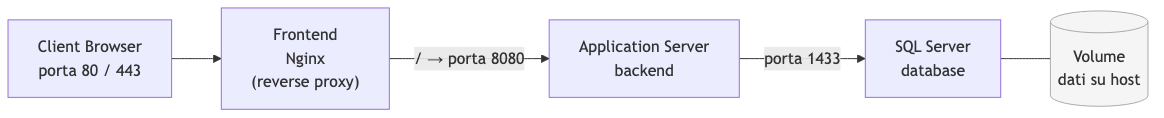
\includegraphics[keepaspectratio,alt={Diagramma Mermaid}]{images/mermaid-lezione-15-virtualizzazione-01.png}}
\emph{Fig. --- Architettura di un'applicazione multi-container con
Docker Compose: Nginx riceve le connessioni esterne e le inoltra al
backend; il database monta un volume host per la persistenza.}

\subsection{Orchestrazione: Kubernetes}\label{orchestrazione-kubernetes}

Una volta che si è in grado di eseguire più container, nasce
spontaneamente il bisogno di orchestrarli su più macchine. Kubernetes
(abbreviato K8s) nasce in Google proprio per questo: scalare i servizi
di ricerca su cluster di migliaia di macchine. Il caso d'uso originale è
semplice: se ho 1000 richieste concorrenti, voglio istanziare
automaticamente N repliche del container che serve la richiesta e
bilanciarle.

\begin{calloutdefinition}{Kubernetes}

Piattaforma open source per l'orchestrazione di container su cluster di
macchine. Permette di definire lo stato desiderato del sistema (numero
di repliche, risorse allocate, regole di networking) e si occupa
autonomamente di mantenerlo.

\end{calloutdefinition}

L'architettura è composta da un \textbf{control plane} (nodo master che
coordina tutto il cluster) e da \textbf{worker node} su cui girano i
container. I container sono raggruppati in \textbf{pod} --- la più
piccola unità deployabile in Kubernetes, tipicamente un container o un
gruppo strettamente accoppiato.

\begin{callouttip}{Canary deployment e rolling updates}

Kubernetes permette di avere contemporaneamente la versione 1 e la
versione 2 di un servizio. Il reverse proxy in ingresso (Ingress
controller) decide la percentuale di traffico da inviare a ciascuna
versione. Si aggiorna così gradualmente il software senza interruzioni
di servizio (rolling update) o si testa la nuova versione su una piccola
percentuale di utenti (canary deployment).

\end{callouttip}

\begin{center}\rule{0.5\linewidth}{0.5pt}\end{center}

\section{Virtualizzazione}\label{virtualizzazione}

\subsection{VM vs Container: la differenza
fondamentale}\label{vm-vs-container-la-differenza-fondamentale}

La differenza chiave è il livello di isolamento: i container condividono
il kernel del sistema operativo host; le VM no. Una VM contiene il
proprio sistema operativo completo, compreso il kernel. Questo significa
che:

\begin{itemize}
\tightlist
\item
  Su una macchina si possono eseguire simultaneamente una VM Linux e una
  VM Windows (impossibile con i container, che devono condividere il
  kernel dell'host)
\item
  Una vulnerabilità del kernel non attraversa il confine della VM
\item
  Le VM hanno overhead maggiore (dimensione su disco, memoria, tempo di
  avvio)
\end{itemize}

\begin{calloutnote}{WSL2 e i container Linux su Windows}

Su Windows, i container Linux vengono eseguiti dentro una VM Linux
leggera gestita da Hyper-V (WSL2). Non è una violazione del principio: i
container condividono il kernel della VM Linux, non direttamente il
kernel Windows.

\end{calloutnote}

\subsection{L'Hypervisor}\label{lhypervisor}

L'\textbf{hypervisor} è il software che implementa la virtualizzazione:
prende le risorse fisiche della macchina (CPU, memoria, rete, storage) e
le suddivide in slice assegnate a ciascuna VM. È responsabile di:

\begin{itemize}
\tightlist
\item
  \textbf{Scheduling della CPU}: distribuire i core fisici tra le VM
\item
  \textbf{Gestione della memoria}: isolare gli spazi di indirizzamento
\item
  \textbf{I/O virtualizzato}: presentare a ogni VM disk controller,
  interfacce di rete e altri dispositivi come se fossero fisici
\item
  \textbf{Virtual console}: permettere l'accesso grafico alla VM
\end{itemize}

\pandocbounded{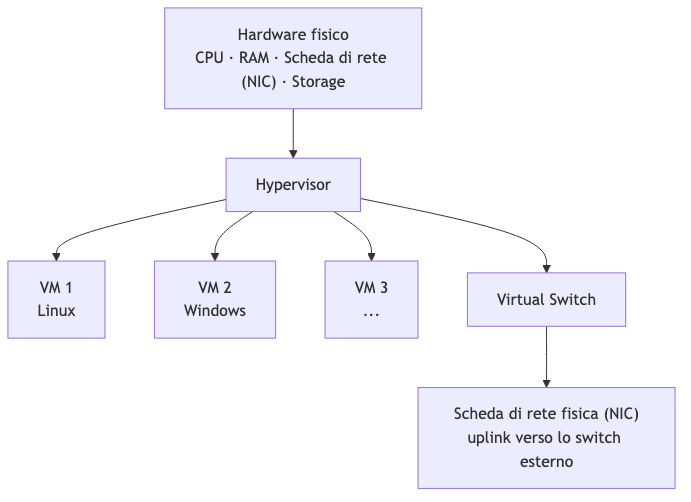
\includegraphics[keepaspectratio,alt={Diagramma Mermaid}]{images/mermaid-lezione-15-virtualizzazione-02.png}}
\emph{Fig. --- Architettura di un sistema di virtualizzazione:
l'hypervisor si interpone tra l'hardware fisico e le VM, esponendo
risorse virtualizzate a ciascuna.}

\subsection{Il Virtual Switch}\label{il-virtual-switch}

Accanto all'hypervisor, il \textbf{virtual switch} è il componente che
rende le VM indistinguibili da macchine fisiche dal punto di vista della
rete. Poiché più VM girano sullo stesso host fisico, serve
un'infrastruttura di rete interna che:

\begin{itemize}
\tightlist
\item
  Assegni a ogni VM un'identità di rete completa (MAC address, IP, VLAN)
\item
  Gestisca il traffico est-ovest tra VM dello stesso host senza passare
  dalla scheda di rete fisica (traffico puramente in-memory, molto più
  veloce)
\item
  Colleghi le VM alla rete fisica usando la scheda di rete fisica
  dell'host come uplink verso lo switch esterno
\end{itemize}

Il virtual switch implementa in software le stesse funzionalità di un
switch fisico: broadcast domain, VLAN tagging, forwarding basato su MAC.
In VMware questo componente si chiama \textbf{vSwitch} (o
\textbf{Distributed Switch} nelle configurazioni enterprise).

\subsection{Live Migration}\label{live-migration}

La capacità più potente della virtualizzazione è la \textbf{live
migration} (chiamata \textbf{vMotion} in VMware): spostare una VM in
esecuzione da un server fisico a un altro \textbf{senza interruzione del
servizio}.

\begin{callouttip}{Perché la live migration è rivoluzionaria}

Un sito web che serve pagine può essere spostato da una macchina fisica
a un'altra mentre continua a rispondere alle richieste HTTP. Questo
rende possibile la manutenzione dell'hardware senza downtime, il
bilanciamento del carico tra server e la gestione automatica dei guasti.
È la tecnologia che ha reso il cloud computing economicamente viable.

\end{callouttip}

Il meccanismo si basa sul fatto che lo stato completo di una VM
(memoria, registri CPU, stato dei device) è una struttura dati nel
software dell'hypervisor. Copiare questa struttura da un host all'altro,
sincronizzare le ultime modifiche e commutare il controllo è
tecnicamente complesso ma possibile. Lo storage condiviso (SAN o NAS)
elimina il problema di dover spostare anche i disk file.

\subsection{CPU Virtualization: anelli e istruzioni
hardware}\label{cpu-virtualization-anelli-e-istruzioni-hardware}

Il problema tecnico più sottile della virtualizzazione è la
\textbf{virtualizzazione della CPU}. Un kernel di sistema operativo
esegue istruzioni privilegiate che accedono direttamente all'hardware
(gestione degli interrupt, manipolazione della memoria fisica,
configurazione del timer). Se si esegue un kernel ``ospite'' dentro una
VM, queste istruzioni devono essere intercettate e gestite
dall'hypervisor prima di raggiungere la CPU fisica.

Le CPU x86 (e ARM) non hanno solo due livelli di privilegio
(supervisor/user): l'Intel 386 ne aveva già 16, chiamati \textbf{ring}
(da ring 0, il più privilegiato, a ring 15). Il kernel normalmente gira
in ring 0 e le applicazioni in ring 3.

Le prime implementazioni di virtualizzazione sfruttavano questi ring
intermedi per interporre il kernel ospite tra il kernel dell'hypervisor
e le applicazioni, ma era un'architettura fragile. La soluzione
definitiva è arrivata con l'introduzione di \textbf{istruzioni hardware
dedicate alla virtualizzazione}:

\begin{itemize}
\tightlist
\item
  \textbf{Intel VT-x} (Virtualization Technology for x86)
\item
  \textbf{AMD-V} (AMD Virtualization)
\end{itemize}

Queste estensioni aggiungono strutture dati (VMCS su Intel) per salvare
e ripristinare efficientemente lo stato completo di una VM durante i
context switch tra VM diverse, interrupt virtuali separati da quelli
fisici, e timer virtuali indipendenti.

\begin{calloutwarning}{Context switch tra VM vs tra processi}

Un context switch tra processi salva/ripristina i registri del processo.
Un context switch tra VM deve salvare/ripristinare l'intero stato del
kernel ospite (registri + stato MMU + interrupt controller virtuale +
timer). Senza supporto hardware è un'operazione ordini di grandezza più
costosa.

\end{calloutwarning}

\subsection{I principali hypervisor}\label{i-principali-hypervisor}

\begin{calloutnote}{Panorama dei vendor}

\begin{itemize}
\tightlist
\item
  \textbf{VMware} (ora Broadcom): leader storico del mercato enterprise.
  Fondato nel 1997-98, acquisito da Dell tramite EMC², poi ceduto a
  Broadcom. Il cambio di ownership ha portato a una riorganizzazione
  radicale del licensing che ha spinto molti clienti a cercare
  alternative --- operazione resa difficile dalla maturità tecnica
  insostituibile di VMware in ambito enterprise.
\item
  \textbf{Hyper-V} (Microsoft): integrato in Windows Server e nelle
  versioni Pro/Enterprise di Windows. Microsoft è stata per un periodo
  il maggior contributore al kernel Linux, contribuendo i moduli per la
  virtualizzazione tramite Hyper-V (usati anche da WSL2).
\item
  \textbf{KVM} (Kernel-based Virtual Machine): modulo integrato nel
  kernel Linux; base di molte distribuzioni cloud, incluso OpenStack.
\item
  \textbf{Proxmox}: soluzione open source basata su KVM, usata molto in
  ambienti homelab e PMI. Non raggiunge le prestazioni e la maturità di
  VMware in ambito enterprise.
\end{itemize}

\end{calloutnote}

\subsection{Snapshot e Checkpoint}\label{snapshot-e-checkpoint}

Un \textbf{checkpoint} (o snapshot) è una fotografia istantanea dello
stato completo di una VM in un dato momento: contenuto della memoria,
stato dei registri CPU, stato del disco. Viene implementato attraverso
lo stesso meccanismo del filesystem differenziale: al momento dello
snapshot, il file del disco virtuale viene congelato e tutte le
scritture successive vanno in un nuovo file differenziale.

\begin{callouttip}{Demo: snapshot e ripristino}

Durante la lezione il professore dimostra la potenza degli snapshot: 1.
Crea una VM Ubuntu su Hyper-V con un virtual disk VHDX 2. Installa
Ubuntu 3. Prende un checkpoint (il file disco si divide: base frozen +
differenziale attivo) 4. Esegue \texttt{rm\ -rf\ /} all'interno della
VM, distruggendo il filesystem 5. Ripristina il checkpoint precedente →
la VM riparte esattamente nello stato in cui era prima del disastro,
memoria inclusa

\end{callouttip}

\begin{calloutwarning}{Performance overhead degli snapshot}

Ogni accesso al disco di una VM con snapshot attivi richiede una ricerca
a cascata attraverso i layer: prima nel differenziale corrente, poi in
quello precedente, e così via. Più snapshot ci sono, più operazioni I/O
multiple si sommano per ogni accesso. Mantenere snapshot a lungo su VM
in produzione (che scrivono continuamente sul disco per aggiornamenti,
log, ecc.) degrada significativamente le prestazioni e aumenta lo spazio
su disco ben oltre la dimensione nominale allocata alla VM. È una
cattiva pratica comune nei team di datacenter operation.

\end{calloutwarning}

\newpage

\chapter{Virtualizzazione 2 --- Live Migration e Gestione del Datacenter
Virtuale}\label{virtualizzazione-2-live-migration-e-gestione-del-datacenter-virtuale}

La lezione riprende il filo della virtualizzazione affrontando i
meccanismi interni dell'hypervisor, le operazioni che questo rende
possibili --- in particolare la \textbf{live migration} --- e le
conseguenze architetturali che queste capacità hanno avuto sull'intera
industria del cloud. Il professore dimostra tutto in diretta su un
cluster reale dell'Università di Pisa.

\begin{center}\rule{0.5\linewidth}{0.5pt}\end{center}

\section{Contesto storico: da IBM agli anni
2000}\label{contesto-storico-da-ibm-agli-anni-2000}

La virtualizzazione non è un'invenzione recente. Il sistema operativo
\textbf{VM/CMS} di IBM, apparso negli anni '70, era già un sistema di
virtualizzazione completo: permetteva di far girare multiple istanze
indipendenti di un sistema monoprogrammato sullo stesso mainframe
fisico. L'idea precede persino il concetto moderno di processo.

\subsection{Emulazione: il predecessore
pratico}\label{emulazione-il-predecessore-pratico}

Prima che la virtualizzazione si affermasse, la soluzione dominante per
eseguire software scritto per un'architettura diversa era
l'\textbf{emulazione}. I Macintosh con CPU PowerPC, ad esempio, usavano
un emulatore x86 per girare software Windows --- più lento, ma
funzionante. La logica dell'emulazione è concettualmente semplice:

\begin{calloutdefinition}{Emulatore}

Un programma che implementa il ciclo \emph{fetch-decode-execute} di una
CPU bersaglio, interpreta ogni istruzione e emula l'effetto di ogni
operazione I/O. Può eseguire codice di qualsiasi architettura su
qualsiasi altra architettura, a patto di accettare un rallentamento
significativo.

\end{calloutdefinition}

Il rallentamento deriva dal fatto che ogni ciclo della CPU emulata
richiede molti cicli della CPU fisica per essere simulato. Storicamente
era accettabile solo per emulare sistemi molto vecchi --- la Legge di
Moore forniva il margine di velocità necessario a compensare
l'inefficienza. Oggi strumenti come \textbf{JSLinux} di Fabrice Bellard
dimostrano che persino sistemi complessi (Linux, Windows 2000) possono
essere emulati all'interno di un browser, incluse CPU di architetture
diverse da quella del dispositivo host.

\begin{calloutnote}{Bug fedeli}

Un emulatore non deve implementare solo la specifica ufficiale di una
CPU, ma anche i suoi bug. Il software reale spesso si affida a
comportamenti non documentati o a quirk storici dell'hardware: un
emulatore che non li riproduce non riesce a far girare quel software
correttamente.

\end{calloutnote}

\subsection{La nascita di VMware (1997) e la virtualizzazione
x86}\label{la-nascita-di-vmware-1997-e-la-virtualizzazione-x86}

Nel 1997, quando VMware fu fondata, le CPU multi-core non esistevano
ancora. Il problema che spinse a creare il primo hypervisor era
pragmatico: un commesso viaggiatore doveva dimostrare architetture
client-server senza connessione internet affidabile. La soluzione fu
eseguire sia il client che il server sulla stessa macchina laptop --- ma
in modo isolato.

Emulare una CPU x86 sopra un'altra CPU x86 è tecnicamente possibile ma
lento. L'insight chiave di VMware fu diverso: se il codice gira già
sulla stessa architettura, non serve emulare le istruzioni --- basta
trovare un meccanismo per \emph{preemptare} il codice della macchina
virtualizzata e lasciarlo girare direttamente sulla CPU fisica,
intervenendo solo quando necessario (accessi privilegiati, I/O, cambio
di contesto).

\pandocbounded{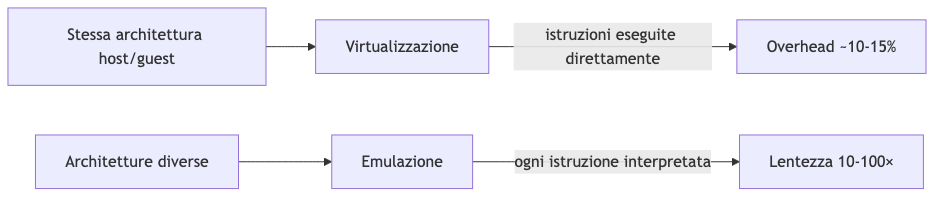
\includegraphics[keepaspectratio,alt={Diagramma Mermaid}]{images/mermaid-lezione-16-virtualizzazione-2-live-migration-e-gestione-01.png}}
\emph{Fig. --- Emulazione vs virtualizzazione: il discriminante è la
compatibilità di architettura.}

\begin{center}\rule{0.5\linewidth}{0.5pt}\end{center}

\section{Perché la virtualizzazione si è
affermata}\label{perchuxe9-la-virtualizzazione-si-uxe8-affermata}

L'esplosione della virtualizzazione nei datacenter avviene attorno al
\textbf{2003-2004}, per una ragione strutturale: l'hardware cresceva più
velocemente del software. I server dell'epoca erano già troppo potenti
per le applicazioni disponibili. Un web server o un mail server, essendo
workload \textbf{IO-bound}, teneva la CPU occupata una piccola
percentuale del tempo: il processore aspettava il disco o la rete, non
elaborava.

In questo contesto, far girare una singola applicazione per server era
uno spreco enorme. La virtualizzazione offriva la risposta: eseguire
decine di servizi isolati sulla stessa macchina fisica, sfruttando i
core altrimenti inattivi.

\begin{callouttip}{Perché non semplici processi?}

I processi condividono sistema operativo, librerie e kernel. Due
applicazioni che richiedono versioni diverse della stessa libreria non
possono coesistere facilmente. Una patch di sicurezza a un componente
richiede il riavvio dell'intera macchina. Una compromissione del web
server può propagarsi al database. La VM risolve tutti e tre i problemi
grazie all'\textbf{isolamento completo}.

\end{callouttip}

Il secondo catalizzatore fu l'arrivo delle \textbf{CPU multi-core}
attorno al 2006. Il software dell'epoca era quasi tutto single-threaded
--- il multithreading era considerato programmazione avanzata. La
virtualizzazione diventò il modo principale per sfruttare i core
aggiuntivi senza riscrivere le applicazioni: ogni VM occupava uno o più
core separati.

L'overhead introdotto dall'hypervisor moderno è stimato attorno al
\textbf{10-15\%} --- ben speso dato il ritorno in termini di isolamento,
flessibilità e gestibilità.

\begin{center}\rule{0.5\linewidth}{0.5pt}\end{center}

\section{L'hypervisor per ambienti
server}\label{lhypervisor-per-ambienti-server}

Il software di virtualizzazione desktop (VirtualPC, VMware Workstation)
era pensato per eseguire sistemi operativi con interfaccia grafica,
audio, USB. L'\textbf{hypervisor} per server è un sistema completamente
diverso: nessuna console grafica, gestione solo via rete, ottimizzato
per eseguire decine o centinaia di VM headless.

\subsection{La vCPU e la gestione dell'instruction
set}\label{la-vcpu-e-la-gestione-dellinstruction-set}

Ogni VM riceve una o più \textbf{vCPU} --- CPU virtuali che mappano sui
core fisici del server. La vCPU non è semplicemente un core fisico
dedicato: è un'astrazione configurabile. In particolare, l'hypervisor
può dichiarare alla VM un sottoinsieme delle istruzioni disponibili
sulla CPU fisica.

Questo è cruciale per la \textbf{live migration}. Se una VM utilizza
istruzioni AVX-512 disponibili solo su alcuni modelli Intel, non può
essere spostata su un server con una CPU più vecchia che non supporta
quelle istruzioni. Configurando la vCPU per esporre solo le istruzioni
comuni al set minimo tra sorgente e destinazione, si garantisce la
portabilità.

Analogamente, l'hypervisor può configurare la topologia \textbf{NUMA}
percepita dalla VM: quanti socket, quanti nodi NUMA, quanta memoria per
nodo. La VM non vede la topologia reale del server fisico --- vede solo
ciò che l'hypervisor le mostra.

\subsection{Due sistemi operativi all'avvio di
Windows}\label{due-sistemi-operativi-allavvio-di-windows}

Un fatto poco noto: Windows, all'avvio, lancia \textbf{due sistemi
operativi}, non uno. Il primo è un micro-OS molto piccolo, senza
console, che prende il controllo dell'hardware dedicato alla protezione
delle chiavi crittografiche --- quelle usate per BitLocker, TPM,
transazioni finanziarie. Questo micro-OS è chiamato internamente
\textbf{Secure World} (o Virtual Secure Mode). Solo dopo averlo avviato,
lancia Windows normale, che gira accanto a lui in modalità
virtualizzata.

\begin{callouttip}{Perché due OS?}

Il software non è perfetto. Se un attaccante ottiene privilegi kernel su
Windows, normalmente può leggere qualsiasi area di memoria, incluse le
chiavi crittografiche. Con il modello a due OS, le chiavi risiedono nel
Secure World, inaccessibile anche al kernel Windows. Il Secure World è
esposto solo attraverso API ben definite, rendendo molto più difficile
l'esfiltrazione.

\end{callouttip}

Lo stesso principio vale per \textbf{Windows Subsystem for Linux
(WSL2)}: anche qui gira un kernel Linux completo all'interno di Windows,
sfruttando le stesse tecniche di virtualizzazione. Sul laptop del
professore (ARM con processore Apple) gira anche un layer di emulazione
x86 integrato in Windows, dimostrando la coesistenza di tre livelli: ARM
nativo, x86 emulato, Linux virtualizzato.

\begin{center}\rule{0.5\linewidth}{0.5pt}\end{center}

\section{Operazioni fondamentali sulle
VM}\label{operazioni-fondamentali-sulle-vm}

\subsection{Pause e Resume}\label{pause-e-resume}

Un hypervisor può fermare completamente l'esecuzione di una VM in
qualsiasi momento. Questo è possibile perché un sistema operativo è, in
ultima analisi, codice che viene eseguito dal ciclo fetch-execute. Se si
interrompe quel ciclo e si conserva lo stato --- i registri della CPU
--- il sistema operativo non ha alcun modo di accorgersi che il tempo si
è fermato. Alla ripresa, riprende esattamente da dove si era fermato.

\begin{calloutdefinition}{Stato completo di una VM}

Lo stato completo di una VM è composto da tre elementi: (1) i
\textbf{registri della CPU} inclusi quelli di sistema, (2) il contenuto
della \textbf{memoria RAM} allocata alla VM, (3) lo stato del
\textbf{disco virtuale}. Conservare tutti e tre equivale a poter
ricreare fedelmente la VM in qualsiasi momento futuro.

\end{calloutdefinition}

\subsection{Snapshot}\label{snapshot-1}

Uno \textbf{snapshot} è una fotografia del stato completo della VM in un
istante dato. Tecnicamente si realizza con una combinazione di: - Copia
dei registri CPU - Copia della memoria (o riferimento CoW ---
Copy-on-Write) - Disco differenziale: da quel momento in poi, le
scritture sul disco vanno in un file differenziale separato; il disco
originale resta intatto come ``base''

L'insieme di snapshot forma una catena che permette di tornare a
qualsiasi punto precedente nel tempo, esattamente come i commit di un
sistema di versionamento.

\subsection{Integration Services}\label{integration-services}

L'hypervisor espone alla VM un insieme di servizi di integrazione che
vanno oltre la semplice emulazione hardware:

\begin{itemize}
\tightlist
\item
  \textbf{Sincronizzazione del clock}: la VM usa il clock dell'host.
  Cruciale perché Kerberos (il protocollo di autenticazione usato in
  Active Directory e nei datacenter) richiede che tutti i sistemi
  abbiano lo stesso orario con margine inferiore a 5 minuti. Un clock
  desincronizzato impedisce l'autenticazione.
\item
  \textbf{Heartbeat}: la VM invia periodicamente un segnale
  all'hypervisor. Se il heartbeat cessa, l'hypervisor sa che il kernel
  della VM è bloccato e può intervenire con un riavvio forzato ---
  fondamentale per la business continuity.
\item
  \textbf{Shutdown graceful}: l'hypervisor può inviare alla VM il
  segnale equivalente alla pressione del tasto power, permettendo uno
  spegnimento pulito anziché un kill brutale.
\item
  \textbf{Backup senza contention}: sospendendo brevemente la VM,
  l'hypervisor può eseguire un backup coerente del disco senza race
  condition, anche con il sistema in esecuzione.
\end{itemize}

\begin{center}\rule{0.5\linewidth}{0.5pt}\end{center}

\section{Live Migration}\label{live-migration-1}

La \textbf{live migration} è probabilmente la funzionalità più
importante introdotta dalla virtualizzazione nell'industria del
datacenter. Permette di spostare una VM da un server fisico a un altro
\textbf{mentre è in esecuzione}, con un'interruzione percepibile
dell'ordine di qualche millisecondo --- del tutto compatibile con i
normali glitch di rete.

\subsection{Cold migration vs live
migration}\label{cold-migration-vs-live-migration}

La \emph{cold migration} è concettualmente semplice: si spegne la VM, si
copiano i file del disco e della memoria sul server destinazione, si
riavvia. La VM è offline per tutta la durata della copia.

La \emph{live migration} mantiene la VM operativa durante quasi tutta la
fase di trasferimento. Il problema tecnico è che la VM continua a
modificare memoria e disco durante la copia, rendendo impossibile
ottenere uno snapshot coerente senza un intervento coordinato.

\pandocbounded{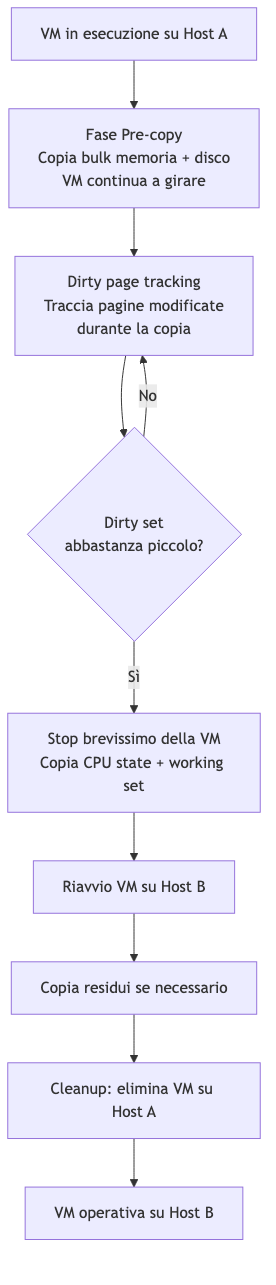
\includegraphics[keepaspectratio,alt={Diagramma Mermaid}]{images/mermaid-lezione-16-virtualizzazione-2-live-migration-e-gestione-02.png}}
\emph{Fig. --- Il processo di live migration in sei fasi: pre-copy con
dirty tracking, stop-copy, riavvio e cleanup.}

\subsection{Fase 1: Pre-copy con dirty page
tracking}\label{fase-1-pre-copy-con-dirty-page-tracking}

La prima fase è la più lunga. L'hypervisor comincia a copiare memoria e
disco verso il server destinazione mentre la VM continua a girare.
Durante questa copia, ogni pagina di memoria (o blocco di disco)
modificata dalla VM viene marcata come \textbf{dirty}: deve essere
ricopiata perché il valore già trasferito è diventato obsoleto.

Il meccanismo di \textbf{page fault} dell'hypervisor è lo strumento
chiave: quando la VM prova a scrivere in una pagina già inviata alla
destinazione, si genera un fault che permette all'hypervisor di
aggiornare il tracking.

Con il passare del tempo, se la VM non è troppo ``write-intensive'', il
set di pagine dirty si riduce: la maggior parte della memoria è già
stata copiata e non è stata rimodificata. A questo punto si è pronti per
la fase finale.

\subsection{Fase 2: Stop, copy del working set,
riavvio}\label{fase-2-stop-copy-del-working-set-riavvio}

Quando il dirty set è sufficientemente piccolo --- ogni sistema ha le
proprie soglie --- l'hypervisor \textbf{ferma la VM per un brevissimo
momento}. In questo fermo: 1. Copia i registri CPU 2. Copia le restanti
pagine dirty (il \emph{working set attivo}) 3. Trasferisce il tutto alla
destinazione

Dopodiché, la VM viene \textbf{riavviata sulla destinazione}. Il fermo
dura tipicamente pochi millisecondi --- paragonabile alla latenza di un
roundtrip di rete, o alla preemption che qualsiasi sistema operativo
subisce normalmente durante lo scheduling.

\subsection{Fase 3: Gestione della rete --- il problema dell'ARP
cache}\label{fase-3-gestione-della-rete-il-problema-dellarp-cache}

Quando la VM si sposta su un altro host fisico, il suo indirizzo MAC (e
IP) rimangono invariati --- vanno con la VM. Ma i switch fisici
mantengono una \textbf{ARP cache} che associa ogni MAC address alla
porta fisica su cui lo hanno visto l'ultima volta. Dopo lo spostamento,
quella cache è obsoleta: i pacchetti verrebbero ancora inviati alla
porta del vecchio host.

La soluzione è un meccanismo a due livelli:

\begin{enumerate}
\def\labelenumi{\arabic{enumi}.}
\item
  Il \textbf{virtual switch della destinazione} invia un
  \textbf{gratuitous ARP} --- un messaggio ARP non richiesto che
  annuncia ``il MAC X è ora raggiungibile da questo switch''. Questo
  forza gli switch della rete a invalidare immediatamente le entry
  stantie.
\item
  Nel breve intervallo tra la migrazione e la propagazione del
  gratuitous ARP, il virtual switch della sorgente --- che è un software
  a conoscenza della migrazione --- fa da \textbf{proxy}: i pacchetti
  che arrivano ancora alla sorgente vengono inoltrati alla destinazione
  anziché andare persi.
\end{enumerate}

Il risultato pratico è \textbf{zero packet loss} durante la migrazione.

\pandocbounded{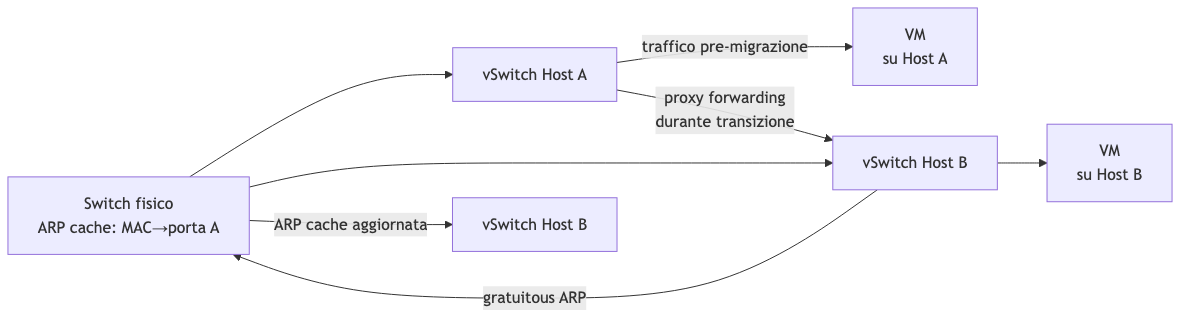
\includegraphics[keepaspectratio,alt={Diagramma Mermaid}]{images/mermaid-lezione-16-virtualizzazione-2-live-migration-e-gestione-03.png}}
\emph{Fig. --- Gestione della rete durante la live migration: forwarding
proxy + gratuitous ARP eliminano la perdita di pacchetti.}

\begin{center}\rule{0.5\linewidth}{0.5pt}\end{center}

\section{Il Cloud come conseguenza della live
migration}\label{il-cloud-come-conseguenza-della-live-migration}

La live migration ha cambiato le regole del gioco nell'industria IT.
Prima di essa, il software era legato all'hardware su cui girava:
aggiornare o sostituire un server significava downtime. Con la live
migration, il legame è spezzato.

\begin{callouttip}{Perché si chiama “Cloud”?}

Il termine ``cloud'' è metaforico: le nuvole in cielo sono un insieme di
vapore acqueo che non si può localizzare con precisione. Analogamente,
nel cloud non si sa --- e non importa sapere --- su quale hardware
specifico girano le proprie risorse. Il cloud provider può muoverle
liberamente, e finché il servizio funziona, per il cliente è
equivalente.

\end{callouttip}

La live migration è la tecnologia abilitante di questa astrazione. Un
server con un disco rotto? Le VM vengono migrate su altri host in pochi
secondi, il server viene spento, sostituito, riavviato --- senza che
nessun utente se ne accorga.

Il professore cita l'esempio concreto del cluster dell'Università di
Pisa: operativo da 8 anni, il primo cluster di 10 nodi è stato
completamente decommissionato e nessuno ha notato, perché le VM sono
state spostate gradualmente con live migration.

\subsection{Container vs VM per la
mobilità}\label{container-vs-vm-per-la-mobilituxe0}

I \textbf{container} --- a differenza delle VM --- non possono essere
migrati a caldo con la stessa facilità. Un processo con il suo stato
interno (socket aperti, memoria allocata, descrittori di file) non può
essere ``congelato'' e ripristinato su un altro host senza serializzare
esplicitamente tutto lo stato. Quella tecnologia (CRIU per Linux) esiste
ma è complessa e non universalmente supportata.

Per questo motivo, il pattern dominante nei datacenter è eseguire
\textbf{container dentro VM}: si ottiene il meglio di entrambi i mondi.
I container forniscono leggerezza e avvio rapido per i workload; la VM
fornisce l'isolamento hardware e la mobilità tramite live migration.

\begin{center}\rule{0.5\linewidth}{0.5pt}\end{center}

\section{Software di gestione: il layer
orchestrator}\label{software-di-gestione-il-layer-orchestrator}

Un singolo hypervisor gestisce le VM di un singolo host. Ma un
datacenter ha decine o centinaia di host. Serve un software che coordini
tutti gli hypervisor da un unico punto di controllo.

Per gli ambienti Microsoft, questo software è \textbf{System Center
Virtual Machine Manager (SCVMM)}. Per VMware, \textbf{vCloud
Foundation}. Questi strumenti permettono di vedere il datacenter come un
unico pool di risorse, eseguire live migration attraverso un'interfaccia
grafica o API, monitorare tutti i cluster, configurare le reti virtuali.

Esistono alternative open source: \textbf{OpenStack} (più orientato alle
API, meno integrato), \textbf{Proxmox} (più simile agli strumenti
commerciali per usabilità). Il professore sottolinea che la scelta tra
open source e commerciale nel datacenter non è solo tecnica:

\begin{calloutwarning}{Open source nel datacenter: una riflessione critica}

Avere il codice sorgente non significa poter risolvere autonomamente
ogni problema. Quando 300 macchine virtuali vanno offline per
un'inconsistenza nello storage, il tempo a disposizione per il debug è
zero. In quel caso, avere un contratto di supporto con ingegneri che
conoscono il prodotto dall'interno vale il suo costo. Il professore
descrive un incidente reale: la risoluzione ha richiesto 6 ore di
escalation su tre continenti (India → Giappone → Messico), dove un
esperto ha usato uno strumento open source per analizzare i metadati del
filesystem e fornire il comando esatto per ripristinare la coerenza.
L'alternativa senza supporto sarebbe stata 4 giorni di restore da
backup.

\end{calloutwarning}

\begin{center}\rule{0.5\linewidth}{0.5pt}\end{center}

\section{Architettura a cluster}\label{architettura-a-cluster}

Un \textbf{cluster} è un insieme di server che condividono risorse e si
coordinano per garantire alta disponibilità. Ogni nodo contribuisce con
CPU, memoria, storage e rete al pool condiviso. L'hypervisor di ciascun
nodo comunica con gli altri per sapere quante risorse sono disponibili,
dove stanno le VM, e cosa fare in caso di guasto.

\pandocbounded{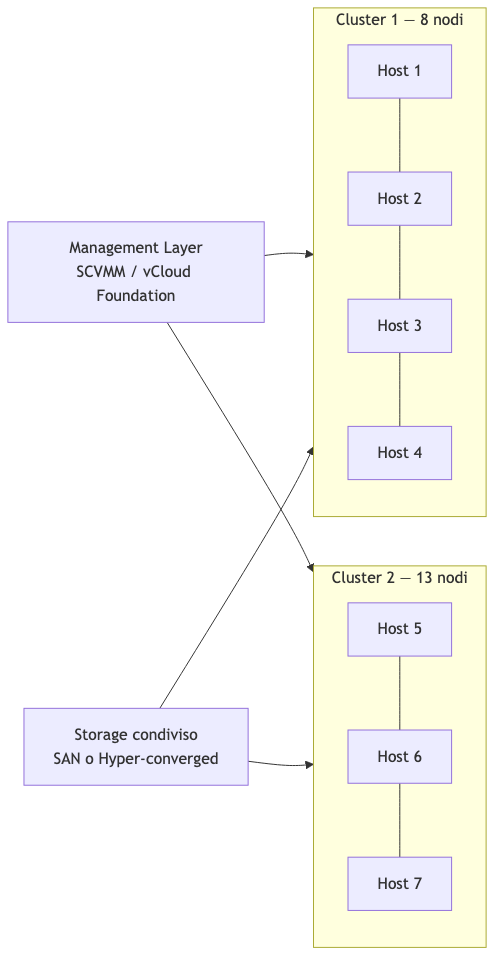
\includegraphics[keepaspectratio,alt={Diagramma Mermaid}]{images/mermaid-lezione-16-virtualizzazione-2-live-migration-e-gestione-04.png}}
\emph{Fig. --- Il datacenter come insieme di cluster gestiti da un layer
di management centralizzato.}

\subsection{Limiti dimensionali del
cluster}\label{limiti-dimensionali-del-cluster}

I cluster non crescono indefinitamente. Il limite pratico è attorno a
\textbf{32 nodi}. La ragione è la complessità della comunicazione
intra-cluster: ogni nodo deve tenersi aggiornato sullo stato di tutti
gli altri. Il pattern di comunicazione è quasi \textbf{quadratico} nel
numero di nodi: raddoppiare i nodi quadruplica quasi la quantità di
messaggi di heartbeat e sincronizzazione dello stato. Oltre una certa
dimensione, il coordinamento introduce latenze non accettabili.

Il \textbf{master role} all'interno del cluster è floating: un nodo
assume il ruolo di master, ma non è fisso. Se il master diventa
irraggiungibile, gli altri nodi usano un protocollo di consenso per
eleggerne uno nuovo. Questo evita il single point of failure che
esisterebbe con un master fisso.

Per scalare oltre i limiti di un singolo cluster, si usano
\textbf{multipli cluster} coordinati dallo stesso management layer.

\begin{calloutnote}{Prerequisito per la live migration intra-cluster}

Tutti i nodi di un cluster devono essere connessi alle \textbf{stesse
reti}. Se una VM è connessa a una specifica VLAN, quella VLAN deve
essere disponibile su ogni host del cluster --- altrimenti la live
migration fallisce perché la VM non può mantenere la sua connettività.

\end{calloutnote}

\begin{center}\rule{0.5\linewidth}{0.5pt}\end{center}

\section{Storage: Hyper-converged vs
SAN}\label{storage-hyper-converged-vs-san}

Il modo in cui lo storage è collegato alle VM ha implicazioni di
performance significative.

\subsection{Hyper-converged infrastructure
(HCI)}\label{hyper-converged-infrastructure-hci}

Nell'architettura \textbf{hyper-converged}, i dischi fisici di ogni
server fanno parte di un pool di storage distribuito. I file delle VM
girano fisicamente sui dischi del server su cui la VM è in esecuzione
--- o sui server più vicini nella rete del cluster. Il traffico tra vCPU
e vDisk viaggia sul bus \textbf{PCIe} interno al server, non sulla rete.

Il software che gestisce il pool distribuito (S2D su Microsoft, vSAN su
VMware) mantiene tipicamente \textbf{3 copie} di ogni blocco di dati su
nodi diversi. Questo garantisce la sopravvivenza al guasto di uno o due
nodi.

\textbf{Vantaggio}: bandwidth massima, latenza minima.
\textbf{Svantaggio}: si usa solo 1/3 dello spazio disco totale
(efficienza 33\%). Le licenze software (Microsoft S2D, VMware vSAN) sono
costose --- talvolta più del hardware stesso.

\subsection{SAN (Storage Area Network)}\label{san-storage-area-network}

Nella configurazione SAN, lo storage è centralizzato in un array
dedicato, raggiungibile via FC o iSCSI. I dischi delle VM risiedono
sulla SAN, non sui server.

\textbf{Vantaggio}: spazio usato più efficiente (RAID tradizionale, meno
overhead di replica); licenze software spesso assenti o più economiche.
\textbf{Svantaggio}: la SAN è un collo di bottiglia. La rete FC o iSCSI
ha larghezza di banda inferiore al PCIe. Con carichi I/O elevati
(database), si nota.

\begin{calloutwarning}{L’impatto dell’AI sui costi dello storage}

Il costo degli storage media (SSD, NVMe) è aumentato significativamente
a causa della domanda AI. Questo ha reso ancora più costosa la replica
×3 dell'HCI, spingendo alcune organizzazioni verso la SAN nonostante le
limitazioni tecniche.

\end{calloutwarning}

\begin{center}\rule{0.5\linewidth}{0.5pt}\end{center}

\section{Virtual Networking e Overlay
Networks}\label{virtual-networking-e-overlay-networks}

\subsection{La complessità a strati}\label{la-complessituxe0-a-strati}

Ogni VM ha una o più \textbf{NIC virtuali} (vNIC). Queste vNIC sono
connesse a un \textbf{virtual switch} software che gira sull'hypervisor
host. Il virtual switch a sua volta è connesso alle NIC fisiche del
server, che sono connesse agli switch fisici della rete.

Ogni strato aggiunge complessità al troubleshooting: seguire il percorso
di un pacchetto richiede di conoscere la configurazione del virtual
switch, le VLAN tagate sulle porte fisiche, e la topologia dello switch
fisico.

\subsection{Il limite delle VLAN e
VXLAN}\label{il-limite-delle-vlan-e-vxlan}

Le VLAN tradizionali (IEEE 802.1Q) hanno un identificatore a 12 bit: al
massimo \textbf{4096 VLAN} distinte su tutta la rete. In un datacenter
con milioni di tenant virtuali, questo è insufficiente.

La soluzione è \textbf{VXLAN} (\emph{Virtual eXtensible LAN}): un
protocollo di overlay che incapsula frame Ethernet layer 2 all'interno
di pacchetti UDP layer 3. L'identificatore VXLAN è a 24 bit: circa
\textbf{16 milioni} di reti virtuali distinte.

\pandocbounded{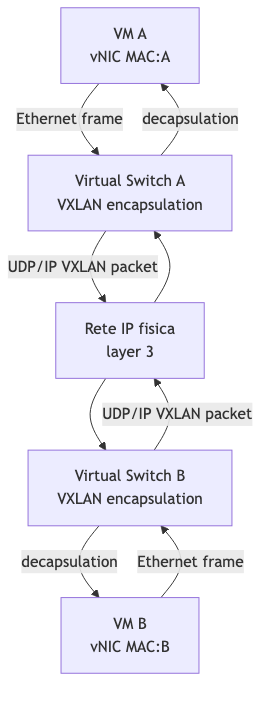
\includegraphics[keepaspectratio,alt={Diagramma Mermaid}]{images/mermaid-lezione-16-virtualizzazione-2-live-migration-e-gestione-05.png}}
\emph{Fig. --- VXLAN: frame Ethernet tra VM incapsulati in UDP/IP,
permettendo LAN virtuali indipendenti dall'infrastruttura fisica.}

\begin{calloutdefinition}{Overlay Network}

Una rete logica costruita sopra una rete fisica esistente, senza
richiedere modifiche all'infrastruttura fisica. Il traffico dell'overlay
appare come normale traffico IP/UDP per gli switch fisici, ma trasporta
frame di reti virtuali separate. Questo permette di creare LAN isolate
per tenant diversi su qualsiasi numero di server nel datacenter.

\end{calloutdefinition}

L'overlay network elimina la necessità di configurare VLAN sugli switch
fisici per ogni nuovo tenant --- operazione manuale, lenta, e limitata a
4096 combinazioni. Con VXLAN, la configurazione avviene interamente a
livello software nel virtual switch, da un pannello centralizzato.

\subsection{Ridondanza delle NIC}\label{ridondanza-delle-nic}

Ogni server in un cluster è tipicamente connesso con \textbf{due NIC}
alla rete di produzione (più una terza per il management). Le due NIC
vanno a due switch fisici diversi --- spine-leaf. Se uno switch fisico
cade, il traffico fluisce automaticamente attraverso l'altro link. Il
virtual switch gestisce questa failover in modo trasparente per le VM.

\begin{center}\rule{0.5\linewidth}{0.5pt}\end{center}

\section{Aggregazione delle risorse e visione del
datacenter}\label{aggregazione-delle-risorse-e-visione-del-datacenter}

Mettendo insieme tutti i pezzi, un datacenter virtualizzato si presenta
come:

\begin{itemize}
\tightlist
\item
  Un insieme di \textbf{cluster} di 8-32 host ciascuno
\item
  Ogni host contribuisce CPU, RAM, storage e network al pool del cluster
\item
  I pool di cluster multipli sono gestiti da un unico management layer
\item
  Le VM vengono allocate \emph{draw}ando dalle risorse del pool
\item
  La live migration permette di bilanciare il carico, fare manutenzione
  hardware, e rispondere ai guasti in modo trasparente
\end{itemize}

La virtualizzazione ha completamente \textbf{decoupled il software
dall'hardware}: il software non sa su quale server fisico gira, e non ha
bisogno di saperlo. Il cloud è la manifestazione estrema di questo
principio --- il software non sa nemmeno in quale datacenter fisico
gira.

\begin{calloutnote}{Sintesi}

La virtualizzazione non è solo un modo per far girare più OS sulla
stessa macchina. È l'infrastruttura tecnologica che ha reso possibile il
cloud computing: la live migration garantisce mobilità del workload; il
virtual switch e VXLAN garantiscono portabilità della rete;
l'hyper-convergence massimizza le prestazioni I/O. Il costo pagato ---
10-15\% di overhead CPU, spazio disco triplicato, licenze software --- è
ampiamente giustificato dai vantaggi operativi: manutenzione hardware
senza downtime, disaster recovery automatico, isolamento completo tra
tenant.

\end{calloutnote}

\newpage

\chapter{Cloud Computing}\label{cloud-computing}

Il cloud computing è uno degli argomenti centrali del corso, non solo
perché interessa direttamente l'architettura dei datacenter moderni, ma
perché ha ridefinito il modo in cui le organizzazioni pensano all'IT. Il
professore parte da un punto fondamentale: il cloud non è nato come
tecnologia, ma come \textbf{modello di business}.

\begin{center}\rule{0.5\linewidth}{0.5pt}\end{center}

\section{Origini e contesto storico}\label{origini-e-contesto-storico}

Nei primi anni 2000, Amazon, Microsoft e Google stavano costruendo
datacenter sempre più grandi per supportare picchi stagionali di
traffico (Natale, estate). Fuori dai picchi, i server rimanevano
inutilizzati. Qualcuno --- in particolare Amazon --- ebbe l'idea di
monetizzare quella capacità in eccesso: perché non affittarla a terzi?

Questo segna il momento in cui nasce il cloud: non come invenzione
tecnica, ma come risposta a un problema economico. Google aveva già
offerto qualcosa di simile con BigTable --- la possibilità di pagare per
indicizzare dati usando le infrastrutture di ricerca di Google --- ma
Amazon trovò la ricetta giusta, quella che portò all'AWS che conosciamo
oggi.

Il cambiamento più profondo non era tecnologico ma finanziario: si
passava dalle \textbf{CapEx} (Capital Expenses, spese in conto capitale)
alle \textbf{OpEx} (Operational Expenses, spese operative). Prima,
un'organizzazione comprava server che possedeva; ora paga per un
servizio, e se smette di pagare non le rimane nulla. Questo è un cambio
di paradigma enorme.

\begin{callouttip}{La logica del capex vs opex}

Con CapEx si compra qualcosa che si possiede e ammortizza nel tempo. Con
OpEx si paga per l'uso: se smetti di usare, smetti di pagare. Il cloud
ha spostato la spesa IT verso OpEx, eliminando l'investimento iniziale
ma introducendo una dipendenza continua dal fornitore.

\end{callouttip}

Nella prima ondata cloud, molti Chief Information Officer pensarono di
potersi liberare completamente dell'IT on-premise. La promessa era
allettante: eliminare l'intero reparto IT aziendale delegando tutto al
cloud. Poi arrivarono i problemi:

\begin{itemize}
\tightlist
\item
  \textbf{Sovranità dei dati}: usare cloud US significa che il governo
  americano può accedere ai dati. L'NSA stava spiando anche Angela
  Merkel; la Germania reagì imponendo a Microsoft di creare una società
  tedesca indipendente per gestire i suoi servizi sul territorio.
\item
  \textbf{Banda e latenza}: una risonanza magnetica può produrre 7 TB in
  mezzora. Come si carica tutto sul cloud? Non si può. Con l'avvento
  dell'IoT, controllare un semaforo via cloud introduce una latenza
  inaccettabile.
\item
  \textbf{Nuovi carichi di lavoro}: video, contenuti, documenti sono
  adatti al cloud; sistemi di controllo real-time no.
\end{itemize}

Questi limiti hanno ridimensionato la promessa del ``full cloud'', ma il
cloud è rimasto fondamentale per molti carichi di lavoro.

\begin{center}\rule{0.5\linewidth}{0.5pt}\end{center}

\section{La definizione formale NIST}\label{la-definizione-formale-nist}

Il \textbf{National Institute of Standards and Technology} (NIST)
americano ha fornito la definizione più usata e ancora valida di cloud
computing:

\begin{calloutdefinition}{Cloud Computing (NIST)}

Il cloud computing è un modello per abilitare l'accesso di rete
conveniente e on-demand a un pool condiviso di risorse computazionali
configurabili (reti, server, storage, applicazioni, servizi) che possono
essere rapidamente provisionate e rilasciate con minimo sforzo di
gestione o interazione con il fornitore.

\end{calloutdefinition}

Il nome ``cloud'' è evocativo: non si sa dove fisicamente girino le
proprie risorse, così come non si sa dove sia fisicamente una nuvola nel
cielo. Questa è resa possibile dalla virtualizzazione e dalla live
migration: il proprio servizio può essere spostato fisicamente da un
continente all'altro senza che l'utente se ne accorga.

\begin{center}\rule{0.5\linewidth}{0.5pt}\end{center}

\section{Le 5 caratteristiche essenziali del
cloud}\label{le-5-caratteristiche-essenziali-del-cloud}

Il NIST identifica cinque caratteristiche che devono essere presenti
perché un servizio possa essere definito cloud.

\subsection{On-demand self-service}\label{on-demand-self-service}

Il consumatore può approvvigionare risorse computazionali
unilateralmente, senza interagire con un operatore umano del fornitore.
Si entra in un portale web, si selezionano le risorse, si inserisce la
carta di credito e si ottengono le macchine virtuali in pochi minuti. Su
AWS, per esempio, non esiste alcun processo di approvazione manuale.

\subsection{Broad network access}\label{broad-network-access}

Le capacità sono disponibili attraverso la rete e accessibili tramite
meccanismi standard che supportano client thin e thick: telefoni,
tablet, laptop, workstation. Il corollario critico di questa
caratteristica è che \textbf{senza rete non si ha accesso a nulla}: il
cloud è inutile offline. Tant'è che alcune app pubblicitizzano il
funzionamento offline come feature premium.

\subsection{Resource pooling}\label{resource-pooling}

Le risorse del fornitore sono aggregate in un pool condiviso per servire
più consumatori con un modello \textbf{multi-tenant}. Le risorse fisiche
e virtuali vengono assegnate e riassegnate dinamicamente secondo la
domanda.

Il concetto di \textbf{tenant} è fondamentale: un tenant è l'insieme di
risorse usate da un'organizzazione all'interno del cloud. Un cloud
multi-tenant ospita contemporaneamente l'Università di Pisa,
l'Università di Bologna, e così via, ciascuna con proprie policy di
sicurezza e identità.

Un aspetto importante è la \textbf{location independence}: il cliente in
generale non conosce né controlla dove esattamente si trovano le sue
risorse, ma può specificare la posizione a livello alto (paese,
regione). Per le pubbliche amministrazioni in Italia, è obbligatorio per
legge garantire la residenza dei dati in Europa.

\subsection{Rapid elasticity}\label{rapid-elasticity}

Le risorse possono essere provisionate e rilasciate elasticamente --- in
alcuni casi automaticamente --- per scalare rapidamente verso l'alto e
verso il basso in funzione della domanda. Per il consumatore, le risorse
sembrano \emph{infinite}: è la dimensione del datacenter ad essere così
grande che quasi sempre c'è spazio per un'altra macchina virtuale.

\begin{callouttip}{Elasticità: l’esempio dei videogiochi}

Ubisoft non possiede un proprio datacenter dimensionato per il picco di
lancio dei suoi giochi. Nelle settimane del lancio c'è un ramp-up enorme
di richieste, poi il traffico cala. Se Ubisoft acquistasse hardware per
il picco, lo lascerebbe quasi sempre inutilizzato. Con il cloud invece
si aggiungono risorse durante il picco, si pagano, e si rilasciano
quando il traffico cala.

\end{callouttip}

\begin{callouttip}{Elasticità automatica: il sistema delle tasse}

Il sistema di dichiarazione dei redditi in Italia ha un picco enorme nel
giorno di scadenza (tutti aspettano l'ultimo momento). Con l'elasticità
automatica si può configurare: ``se la latenza delle risposte del web
server supera X, aggiungi un worker; se scende sotto Y, rimuovine uno''.
Il sistema scala da solo, pagando solo per le risorse effettivamente
usate.

\end{callouttip}

È importante distinguere \textbf{scala} (dimensione totale
dell'infrastruttura) da \textbf{elasticità} (capacità di allocare e
deallocare rapidamente su scale temporali brevi). Comprare un server e
venderlo dopo 5 anni non è elasticità; richiedere 1000 CPU e ottenerle
in 5 minuti, per poi rilasciarle in un'ora, lo è.

\subsection{Measured service}\label{measured-service}

I sistemi cloud controllano e ottimizzano automaticamente l'uso delle
risorse tramite capacità di misurazione. L'uso delle risorse può essere
monitorato, controllato e comunicato, garantendo trasparenza sia al
fornitore che al consumatore.

La misurazione avviene a un livello di astrazione: il fornitore non ti
dice su quale specifico disco SSD stanno i tuoi dati, ma ti propone
livelli di servizio --- bronze, silver, gold --- ognuno con garanzie di
throughput diverse (es. bronze: 500 MB/s, silver: 1 GB/s, gold: 5 GB/s).
Paghi per il livello, non per il dispositivo specifico.

\pandocbounded{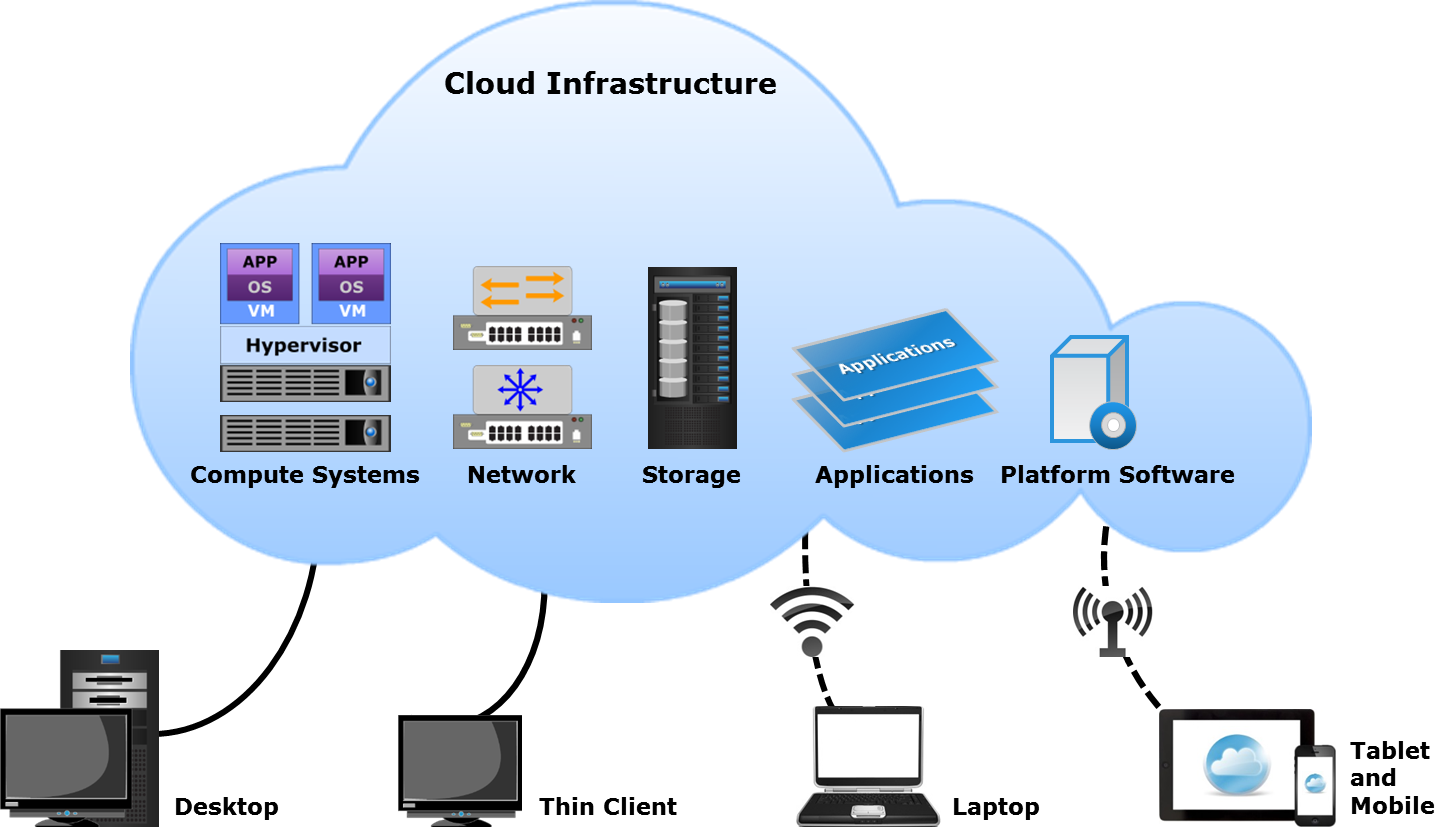
\includegraphics[keepaspectratio]{images/dcdo-cloud-nist-definition.png}}
\emph{Fig. --- Le cinque caratteristiche essenziali del cloud computing
secondo il NIST.}

\begin{center}\rule{0.5\linewidth}{0.5pt}\end{center}

\section{Benefici del cloud}\label{benefici-del-cloud}

Il cloud porta numerosi vantaggi rispetto al modello on-premise
tradizionale.

\textbf{Business agility}: la capacità di rispondere rapidamente alle
opportunità di mercato senza aspettare mesi per acquistare, installare e
configurare hardware.

\textbf{Riduzione dei costi IT}: questa è la promessa più pubblicizzata,
ma anche la più insidiosa. I costi materiali (hardware) sono facilmente
misurabili. I costi del software invece no: il prezzo del software è
quello che il mercato accetta di pagare, non quello che costa produrlo.
Le licenze HCI (Hyper-Converged Infrastructure) sono diventate così
costose che molte organizzazioni stanno tornando allo storage di rete
tradizionale. Attenzione: si può facilmente finire per pagare più di
prima.

\textbf{High availability}: un cloud provider con decine di datacenter
globali può offrire ridondanza e resilienza irraggiungibili per una
singola organizzazione. Se un datacenter viene colpito (per esempio da
un attacco missilistico come nell'esempio citato), il traffico viene
reindirizzato altrove.

\textbf{Flexible scaling}: possibilità di scalare dinamicamente sia
horizontalmente (scale-out) che verticalmente (scale-up).

\textbf{Semplificazione dello sviluppo}: le organizzazioni in passato
mantenevano il doppio dell'infrastruttura --- una per la produzione, una
per il test. Con il cloud, si provisiona un ambiente di test, si usa, si
rilascia.

\begin{center}\rule{0.5\linewidth}{0.5pt}\end{center}

\section{Limiti e svantaggi}\label{limiti-e-svantaggi}

I drawback del cloud sono reali e rilevanti nella pratica.

Il problema della \textbf{sovranità dei dati} è ancora aperto. Il
governo americano rivendica il diritto di accedere a tutti i dati
conservati su cloud di proprietà americana, indipendentemente dalla
posizione geografica. Microsoft, Google e altri hanno fatto azioni
legali per opporsi, con successo parziale. La Germania ha risolto il
problema imponendo a Microsoft di creare una controllata tedesca
indipendente per gestire i dati tedeschi.

Il \textbf{vendor lock-in} è strutturale: se si costruisce tutta la
propria infrastruttura su API proprietarie di un singolo cloud provider,
cambiarlo in seguito è estremamente costoso. La diversificazione degli
investimenti e l'uso di API aperte mitigano il problema, ma non lo
eliminano.

Il \textbf{software licensing} è un territorio complesso: ci sono
professionisti pagati esclusivamente per conoscere i dettagli dei
contratti di licenza Microsoft. Un cambiamento nelle condizioni di
licenza può ribaltare completamente la convenienza economica di una
scelta tecnologica.

\begin{center}\rule{0.5\linewidth}{0.5pt}\end{center}

\section{I modelli di servizio cloud}\label{i-modelli-di-servizio-cloud}

Il NIST formalizza tre modelli di servizio principali che è
indispensabile conoscere. Il professore usa l'analogia della pizza per
renderli immediatamente memorizzabili.

\begin{callouttip}{L’analogia della pizza}

Pensate alla pizza come all'insieme di tutto ciò che serve per mangiare:
ingredienti, impasto, cottura, forno, gas/luce, tavolo, bibita. -
\textbf{On-premise}: si fa tutto a casa (si gestisce tutto). -
\textbf{IaaS}: si compra la pizza surgelata al supermercato e la si
cuoce a casa (il fornitore gestisce fino all'OS, tu gestisci il resto).
- \textbf{PaaS}: si ordina la consegna a domicilio (il fornitore
gestisce tutto tranne la personalizzazione dell'applicazione). -
\textbf{SaaS}: si va al ristorante (il fornitore gestisce tutto, tu usi
solo il servizio finale).

\end{callouttip}

\subsection{Infrastructure as a Service
(IaaS)}\label{infrastructure-as-a-service-iaas}

Il fornitore offre capacità computazionale grezza: processori, storage,
reti. Il consumatore può deployare e far girare qualsiasi software,
inclusi sistema operativo e applicazioni. Il consumatore \textbf{non
gestisce} l'infrastruttura cloud sottostante, ma \textbf{ha controllo}
su OS, storage, applicazioni deployate e --- limitatamente --- sui
componenti di rete (es. firewall).

In pratica: il fornitore installa l'hardware e porta l'OS ``vergine'';
tu lo configuri, aggiorni, gestisci tutta la pila software sopra.

\pandocbounded{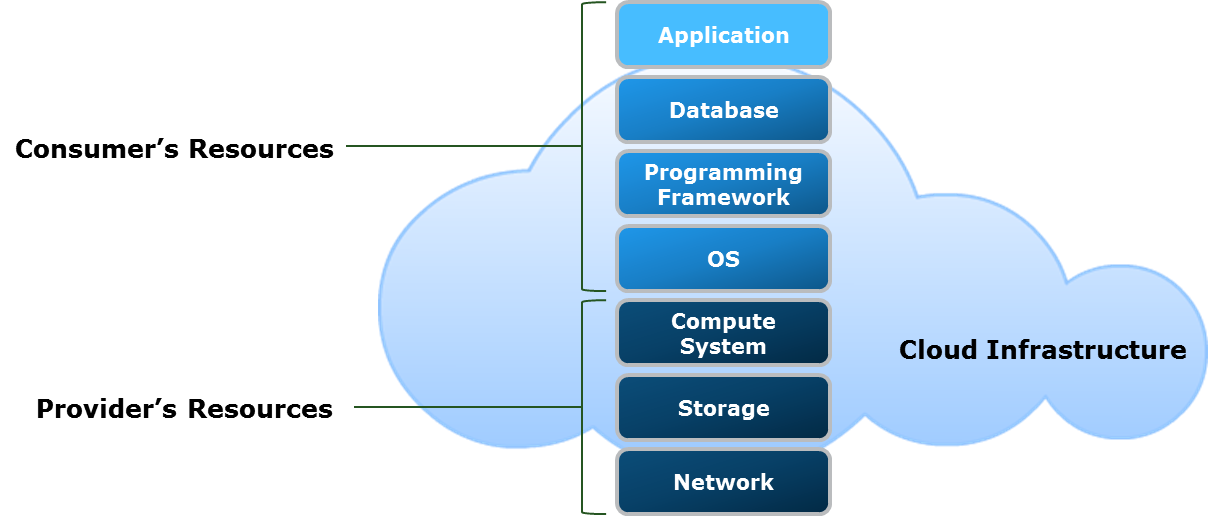
\includegraphics[keepaspectratio]{images/dcdo-cloud-iaas-stack.png}}
\emph{Fig. --- In IaaS il fornitore gestisce hardware e
virtualizzazione; il consumatore gestisce da OS in su.}

\subsection{Platform as a Service
(PaaS)}\label{platform-as-a-service-paas}

Il consumatore deploya applicazioni proprie su un'infrastruttura cloud
usando linguaggi, librerie e tool supportati dal fornitore. Non gestisce
né conosce l'OS sottostante: quello è responsabilità del fornitore. Si
ha controllo solo sull'applicazione.

\textbf{Esempi pratici}: WordPress è un tipico PaaS. Vuoi un sito web?
Non ti preoccupi del web server, del PHP, del sistema operativo.
Acquisti un'istanza WordPress, la personalizzi con plugin e temi tuoi, e
il fornitore gestisce tutto il resto. Salesforce è un altro esempio sul
lato commerciale.

\pandocbounded{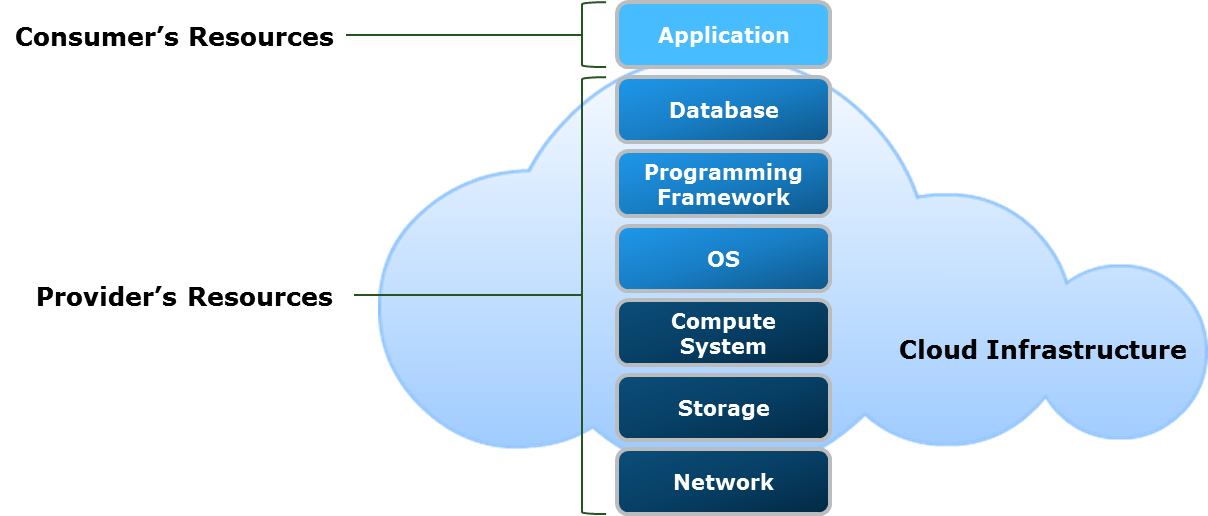
\includegraphics[keepaspectratio]{images/dcdo-cloud-paas-stack.png}}
\emph{Fig. --- In PaaS il fornitore gestisce fino al runtime; il
consumatore gestisce solo l'applicazione.}

\subsection{Software as a Service
(SaaS)}\label{software-as-a-service-saas}

Il consumatore usa direttamente l'applicazione del fornitore girante su
infrastruttura cloud. Non gestisce nulla dell'infrastruttura, della
piattaforma, o dell'applicazione stessa --- solo la configurazione
utente.

\textbf{Esempi}: Gmail è SaaS via browser. Microsoft 365 è SaaS con
applicazioni scaricabili localmente ma intrinsecamente legate al cloud:
se si smette di pagare, le app smettono di funzionare dopo 30 giorni.

\pandocbounded{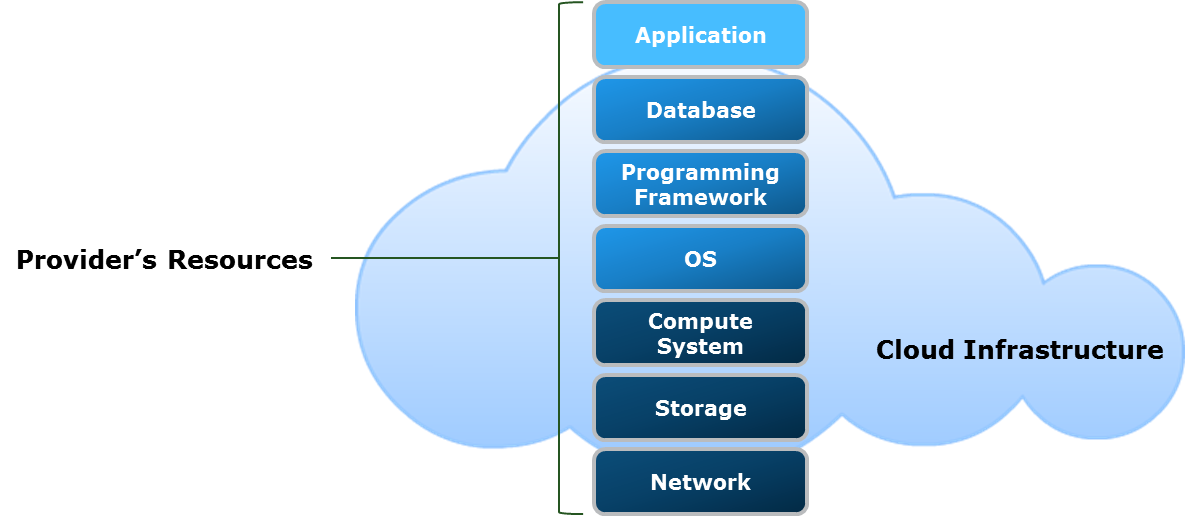
\includegraphics[keepaspectratio]{images/dcdo-cloud-saas-stack.png}}
\emph{Fig. --- In SaaS tutto è gestito dal fornitore; il consumatore usa
solo il prodotto finale.}

\subsection{Cloud Services Brokerage
(CSB)}\label{cloud-services-brokerage-csb}

La \textbf{brokerage} è un livello intermedio che cerca di allocare le
risorse cloud sul fornitore più conveniente tra quelli disponibili (AWS,
Azure, GCP\ldots). In teoria interessante; in pratica, quando Microsoft
e altri hanno adottato la strategia di \emph{matching} automatico dei
prezzi dei concorrenti, il vantaggio economico del broker è quasi
scomparso.

\begin{center}\rule{0.5\linewidth}{0.5pt}\end{center}

\section{I modelli di deployment
cloud}\label{i-modelli-di-deployment-cloud}

Oltre ai modelli di servizio, esistono modelli di \emph{deployment} che
definiscono chi può accedere all'infrastruttura.

\subsection{Public cloud}\label{public-cloud}

L'infrastruttura è provisioned per uso pubblico aperto. Chiunque può
creare un account su AWS, Azure, GCP, Oracle Cloud e allocare risorse,
senza restrizioni. ``Pubblico'' non significa gratuito: significa
accessibile a tutti.

\subsection{Private cloud}\label{private-cloud}

L'infrastruttura è dedicata esclusivamente a una singola organizzazione.
Può essere gestita dall'organizzazione stessa o da terzi, e può esistere
on-premise o off-premise. L'Università di Pisa, per esempio, gestisce un
proprio private cloud.

Il punto chiave: il cloud privato non è privato perché è \emph{owned}
dall'organizzazione, ma perché solo quella organizzazione può allocare
risorse su di esso.

\subsection{Community cloud}\label{community-cloud}

Infrastruttura condivisa tra organizzazioni con mission o requisiti
comuni (es. università italiane, PA europee). Può essere on-premise o
gestita da terzi.

\subsection{Hybrid cloud}\label{hybrid-cloud}

Combinazione di due o più infrastrutture cloud distinte (private,
community, public) che rimangono entità separate ma sono collegate da
tecnologie standardizzate che abilitano la portabilità di dati e
applicazioni.

\begin{callouttip}{UniPi come hybrid cloud}

Quando accedi a un servizio universitario di Pisa, stai probabilmente
usando tre cloud diversi senza saperlo: i servizi di didattica girano
nel datacenter di San Piero (cloud privato UniPi), Alunni gira su Cineca
a Bologna, i documenti sono su OneDrive (Microsoft Azure). Tutto appare
come un'unica esperienza con una singola identità. Questo è hybrid cloud
in pratica.

\end{callouttip}

\pandocbounded{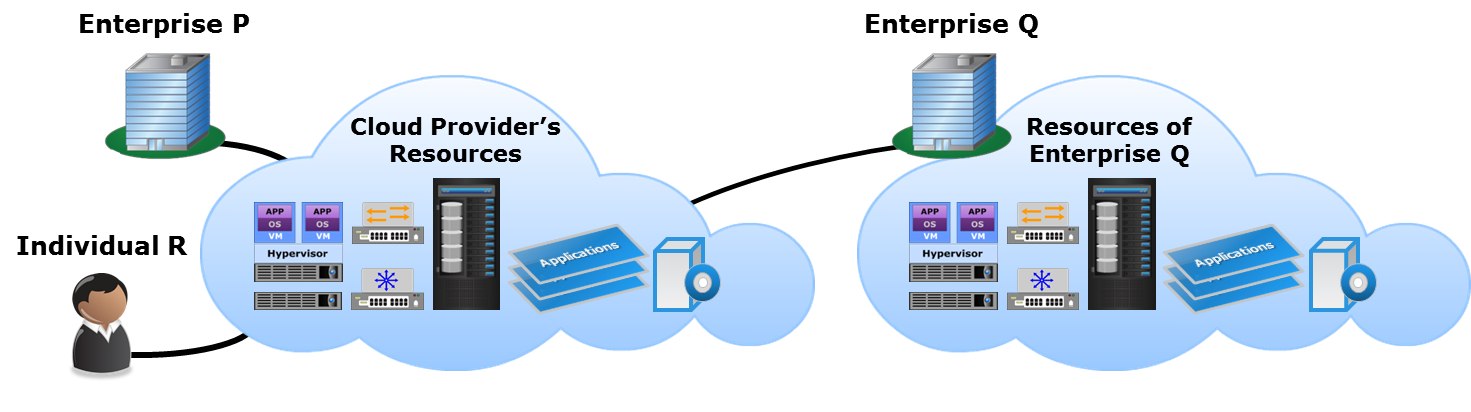
\includegraphics[keepaspectratio]{images/dcdo-cloud-hybrid-model.png}}
\emph{Fig. --- Il modello hybrid cloud combina infrastrutture cloud
diverse collegate da standard aperti.}

\begin{calloutnote}{Impatto del private cloud sull’organizzazione IT}

Il cloud --- anche nella sua versione privata --- ha rivoluzionato il
modello organizzativo dell'IT. Prima ogni progetto acquistava il proprio
server; la capacità inutilizzata era spreco puro. Con il private cloud,
si gestisce un pool condiviso da cui ogni progetto preleva le risorse di
cui ha bisogno, restituendole quando non servono. Tecnologie come VMware
vCloud Foundation, Microsoft Azure Local (ex Azure Stack), e Microsoft
System Center consentono di implementare questo modello on-premise.

\end{calloutnote}

\begin{center}\rule{0.5\linewidth}{0.5pt}\end{center}

\section{Il Cloud Computing Reference
Model}\label{il-cloud-computing-reference-model}

Una volta che le architetture cloud convergono verso pattern comuni, ha
senso definire un \textbf{reference model} --- una mappa condivisa per
descrivere come si organizza un'infrastruttura cloud. Il modello OASIS
(ripreso dal NIST) è ancora valido dopo oltre 12 anni.

\pandocbounded{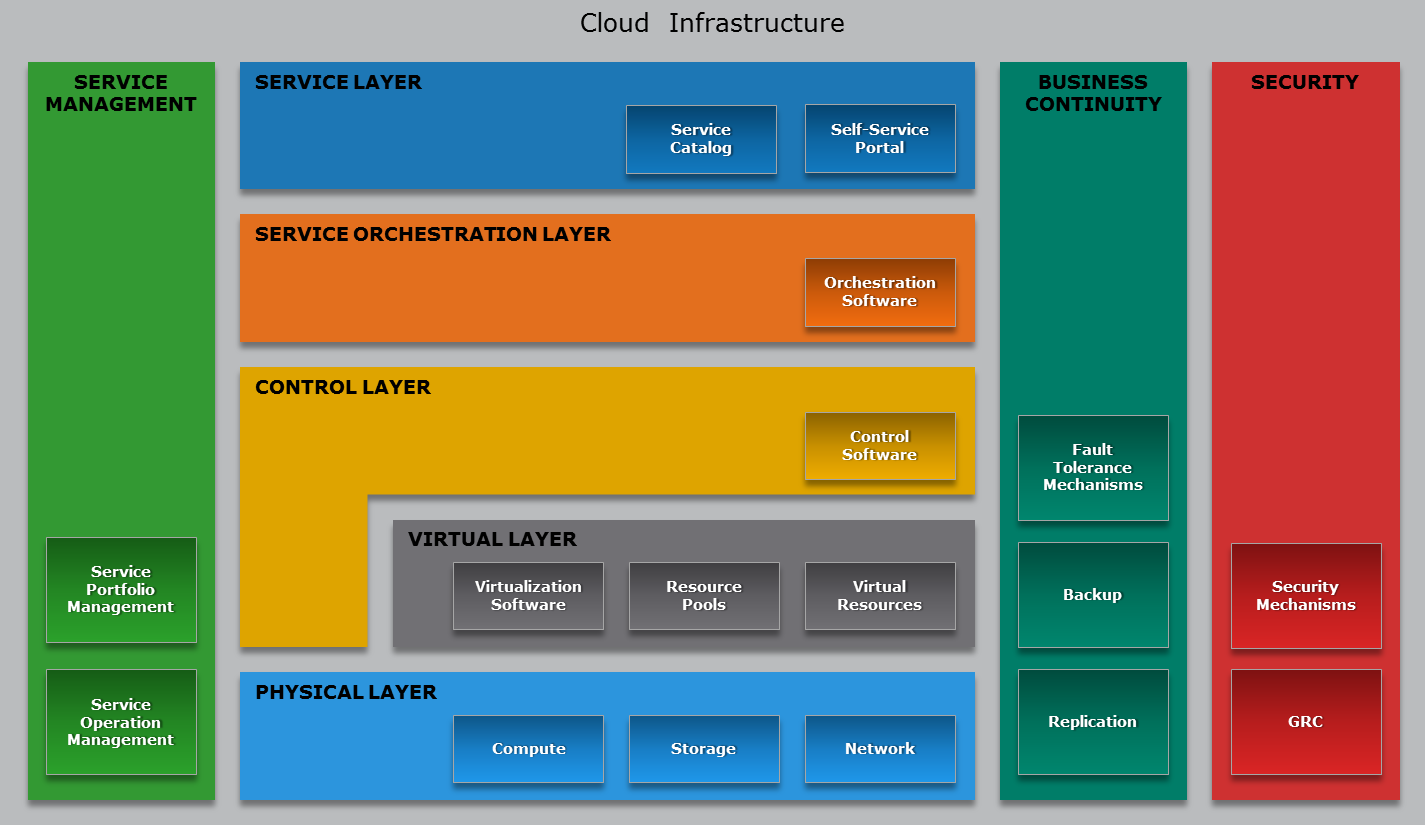
\includegraphics[keepaspectratio]{images/dcdo-cloud-reference-model.png}}
\emph{Fig. --- Il reference model OASIS per il cloud computing: layer
funzionali e aspetti cross-cutting.}

Il modello è strutturato in layer funzionali verticali e aspetti
cross-cutting orizzontali.

\subsection{Physical layer}\label{physical-layer}

Alla base c'è sempre il silicio: compute, storage, network --- tutto ciò
che abbiamo studiato nel corso. La maggior parte del cloud è
implementata tramite virtualizzazione, ma esiste anche il \textbf{bare
metal cloud}: invece di una VM, si provisiiona un intero server fisico
programmandolo via API (es. Redfish). Meno elasticità di granularità
(solo interi server), ma utile per HPC.

\subsection{Virtual layer}\label{virtual-layer}

È il layer cruciale: astrae le risorse fisiche e le presenta come pool
omogeneo da cui allocare slice. Macchine virtuali, storage virtuale,
reti virtuali (VLAN, vSAN) vivono qui. La virtualizzazione è ciò che
rende possibile il resource pooling.

\subsection{Control layer}\label{control-layer}

È l'API che consente di dire ``allocami una VM con queste
caratteristiche'' e di ottenere il risultato. Il control layer sa dove
ci sono risorse libere, le marca come occupate, tiene il libro
contabile. È il ``cervello'' operativo del cloud: quando si fa una
richiesta, il control layer interroga l'inventario, trova capacità
disponibile, alloca e conferma.

\subsection{Administration / Orchestration
layer}\label{administration-orchestration-layer}

Sopra il control layer c'è l'automazione: workflow che definiscono ``se
succede X, esegui Y, poi Z''. Gestisce il provisioning complesso
(allocare una VM, poi aspettare che sia pronta, poi configurarla, poi
avvisare l'utente), il decommissioning hardware (quando un server va in
pensione: wipe dei dischi, rimozione dal configuration database,
segnalazione), e tutto ciò che altrimenti richiederebbe intervento
umano.

\begin{callouttip}{Economia dell’automazione}

I grandi cloud provider gestiscono decine di milioni di server con
pochissimo personale fisico (poche decine di persone per strutture
enormi). Questo è possibile solo perché l'orchestration layer
automatizza praticamente tutto: dalla sostituzione di un disco guasto
alla sostituzione di un intero rack.

\end{callouttip}

\subsection{Service layer}\label{service-layer}

Il layer più alto: il portale web dove l'utente vede il catalogo
servizi, si autentica, seleziona le risorse, paga e le riceve. Traduce
le richieste utente in task che scendono verso l'orchestration e poi il
control layer.

\subsection{Aspetti cross-cutting}\label{aspetti-cross-cutting}

Sicurezza e business continuity non appartengono a un singolo layer:
permeano tutti. La sicurezza deve essere presente a livello fisico
(accesso fisico al datacenter), virtuale (isolamento tra tenant), di
controllo (autenticazione alle API), di orchestration, e di servizio. La
business continuity --- RAID, backup, replication, failover tra
datacenter --- è ugualmente trasversale.

\begin{center}\rule{0.5\linewidth}{0.5pt}\end{center}

\section{Greenfield vs.~Brownfield}\label{greenfield-vs.-brownfield}

Due termini del gergo IT fondamentali:

\textbf{Greenfield}: si parte da zero. Hardware nuovo, sistema deployato
ex novo, test puliti, consegna. È il caso ideale.

\textbf{Brownfield}: si deploya qualcosa in un'infrastruttura già
esistente. Le decisioni prese 10, 20, 30 anni fa condizionano le scelte
odierne. Il professore gestisce servizi universitari da quasi 10 anni e
ancora si confronta con scelte architetturali di decenni fa.

\begin{center}\rule{0.5\linewidth}{0.5pt}\end{center}

\section{Costruire il cloud: non solo
tecnologia}\label{costruire-il-cloud-non-solo-tecnologia}

Una lezione chiave: costruire un'infrastruttura cloud non è solo un
problema tecnico. Ci sono almeno quattro dimensioni non tecniche
altrettanto critiche.

\subsection{Governance}\label{governance}

La governance è la distribuzione attiva di diritti decisionali e
responsabilità tra i vari stakeholder dell'organizzazione. Chi decide
quale servizio attivare? Chi approva il budget? Chi è responsabile in
caso di incidente?

I modelli principali sono tre: \textbf{centralizzato} (un'autorità
centrale governa tutte le business unit), \textbf{distribuito} (ogni
unità ha la propria governance autonoma, tipico di grandi
organizzazioni), \textbf{federato} (combinazione dei due, con autonomia
locale ma coordinamento centrale).

UniPi usa un modello prevalentemente centralizzato: la dimensione
dell'organizzazione lo consente.

Il cloud ha introdotto nuovi ruoli organizzativi: - \textbf{Service
manager}: responsabile di un singolo servizio - \textbf{Account
manager}: gestisce il rapporto con il cliente/utente - \textbf{Cloud
architect}: progetta l'architettura complessiva del cloud -
\textbf{Service operation manager}: responsabile dell'intera
infrastruttura e di tutti i servizi su di essa

\subsection{Finance e procurement}\label{finance-e-procurement}

In un'organizzazione pubblica italiana, la spesa IT è regolata da norme
precise: acquisti diretti fino a \textasciitilde€139.000, oltre tale
soglia si richiede gara europea (€214.000+), con tempi minimi di sei
mesi. Se un server si rompe e bisogna lanciare una gara europea, per sei
mesi non c'è server.

Questo significa che il procurement deve essere \textbf{proattivo}:
bisogna prevedere i fabbisogni futuri, pianificare le gare prima che le
risorse servano. L'Università di Pisa spende circa 6 milioni/anno in IT:
80.000 switch, 2000 access point, datacenter e cloud privato.

Il \textbf{chargeback} è il meccanismo con cui si attribuisce il costo
delle risorse cloud ai reparti o progetti che le usano. Non si chiede
denaro (in un ente pubblico), ma si tiene traccia di chi usa quanto. Il
Dipartimento di Informatica che usa più VM del Dipartimento di Filosofia
dovrebbe ricevere un contributo proporzionalmente maggiore.

Modalità di chargeback nel cloud: - \textbf{Pay-as-you-go}: paghi per
quello che usi - \textbf{Subscription}: abbonamento per un periodo (come
Microsoft 365 annuale) - \textbf{By peak}: si paga per il picco di
utilizzo raggiunto - \textbf{User-based}: costo per utente (il modello
AI aziendale è spesso così: ogni utente ha una quota di token)

\subsection{Service Level Agreement
(SLA)}\label{service-level-agreement-sla}

Quando le proprie risorse sono ``da qualche parte nel cloud'' e non si
può andare fisicamente a verificarle, l'unica garanzia possibile è
quella \textbf{contrattuale}. Uno SLA è la parte del contratto che
specifica i parametri del servizio: disponibilità (es. 99.9\%), schedule
di manutenzione, livelli di performance, tempi di risposta del supporto,
e le compensazioni in caso di violazione.

Gli SLA di tutti i servizi Microsoft online, con versioni storiche e in
tutte le lingue, sono pubblici e consultabili sul sito Microsoft.
Studiarne uno è utile per capire cosa garantisce realmente un cloud
provider.

\subsection{Vendor lock-in}\label{vendor-lock-in}

La dipendenza da un singolo fornitore è un rischio strategico. Se il
fornitore cancella un prodotto, cambia le condizioni di licenza, o
aumenta i prezzi, l'organizzazione è in difficoltà. Strategie di
mitigazione: diversificazione degli investimenti, preferenza per API e
standard aperti.

\pandocbounded{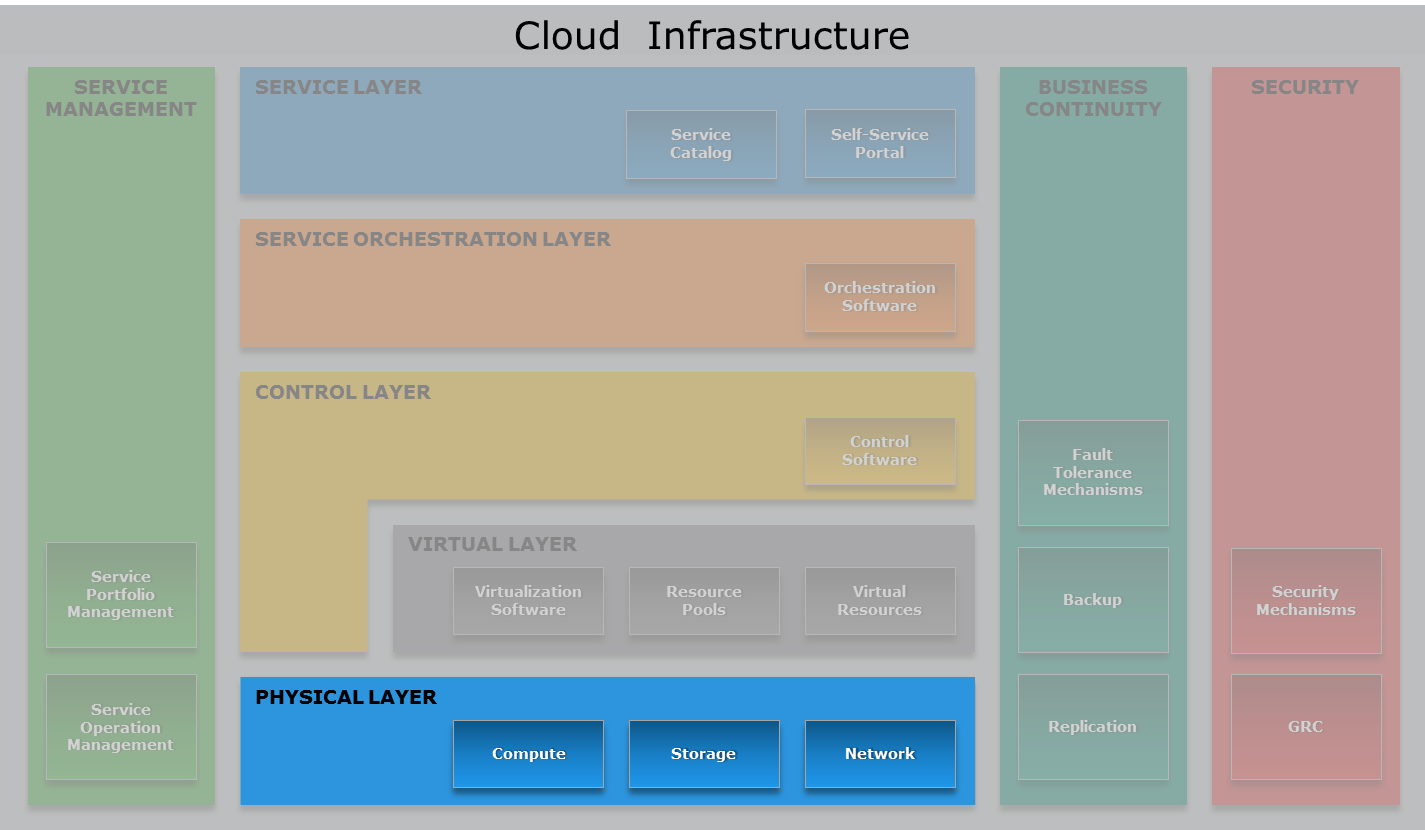
\includegraphics[keepaspectratio]{images/dcdo-cloud-governance-models.png}}
\emph{Fig. --- I tre modelli di governance cloud: centralizzato,
distribuito, federato.}

\begin{center}\rule{0.5\linewidth}{0.5pt}\end{center}

\section{Il physical layer e il virtual layer:
riepilogo}\label{il-physical-layer-e-il-virtual-layer-riepilogo}

Il professore dedica gli ultimi minuti a scorrere rapidamente i layer
fisici e virtuali già trattati nel corso, confermando che i concetti si
incastrano con quanto visto.

Il \textbf{physical layer} comprende compute (server, CPU, GPU), storage
(a blocchi, a file, a oggetti --- unified storage come configurazione
ibrida), e network (Fibre Channel per storage, iSCSI sempre meno usato,
Ethernet convergente). Le note nelle slide originali fanno riferimento
alle tecnologie meccaniche di dischi prima della diffusione degli SSD,
ma le categorie logiche (block, file, object) rimangono attuali.

Il \textbf{virtual layer} è composto da macchine virtuali (file VMDK,
virtual appliance), storage virtuali (LUN thin-provisioned, vSAN), e
reti virtuali. La \textbf{PVLAN} (\emph{Private VLAN}) merita un
dettaglio: è una VLAN che vieta il broadcast orizzontale tra host. Se
siete connessi al Wi-Fi universitario, siete su una PVLAN --- per questo
non potete fare ping tra due device sulla stessa rete wireless: la rete
non consente comunicazione diretta tra client, solo north-south (client
→ gateway).

\begin{calloutnote}{Prossime lezioni}

Il professore ha annunciato che la lezione successiva partirà dal
\textbf{control layer} e dall'\textbf{orchestration layer} --- le parti
veramente nuove rispetto a ciò già coperto nel corso. Poi seguiranno
sicurezza e operazioni, e il venerdì successivo la visita al datacenter
di San Piero.

\end{calloutnote}

\begin{center}\rule{0.5\linewidth}{0.5pt}\end{center}

\newpage

\chapter{Control Layer, Orchestrazione e
SLA}\label{control-layer-orchestrazione-e-sla}

La lezione riprende dal punto in cui si era interrotto il ciclo
precedente, cioè dal \textbf{Control Layer}, l'ultimo strato funzionale
dell'architettura di riferimento del cloud che non era ancora stato
discusso in dettaglio. Il professore chiarisce subito la prospettiva
corretta: dal punto di vista informatico, nessuno degli strati
funzionali del cloud è particolarmente complesso concettualmente. Le
difficoltà reali risiedono nell'hardware, nella topologia e nelle scelte
implementative dei singoli layer. L'obiettivo della lezione è passare
rapidamente sui layer funzionali per poi spostarsi sugli aspetti
trasversali più interessanti: sicurezza, business continuity, service
management e, soprattutto, framework legali e compliance.

\begin{center}\rule{0.5\linewidth}{0.5pt}\end{center}

\section{Il Control Layer}\label{il-control-layer}

\subsection{Posizione
nell'architettura}\label{posizione-nellarchitettura}

Il control layer si inserisce sopra il virtual layer (o direttamente
sopra il physical layer, in assenza di virtualizzazione). Riceve
richieste dagli strati superiori --- service e orchestration layer --- e
si occupa di provisioning delle risorse fisiche e virtuali necessarie
per soddisfarle.

\pandocbounded{\includegraphics[keepaspectratio,alt={Cloud Infrastructure Reference Model con Control Layer evidenziato}]{../../../General/Images and Documents/dcdo_cloud_reference_model_control_layer.png}}
\emph{Fig. --- Il Cloud Reference Model con il Control Layer evidenziato
(in giallo). Sopra ci sono Service Layer e Orchestration Layer; sotto il
Virtual Layer e il Physical Layer.}

\begin{calloutdefinition}{Control Layer}

Include gli strumenti software responsabili di gestire e controllare
l'infrastruttura cloud sottostante, abilitando il provisioning delle
risorse IT per la creazione di servizi cloud.

\end{calloutdefinition}

\subsection{Il Control Software}\label{il-control-software}

Il control software lega insieme le risorse sottostanti. Le sue funzioni
principali sono: \textbf{resource pooling}, \textbf{allocazione
dinamica} delle risorse, \textbf{ottimizzazione dell'utilizzo} e
gestione centralizzata di tutti gli asset. Quest'ultima caratteristica
spiega perché questo software è stato adottato da moltissime
organizzazioni enterprise anche al di fuori di contesti cloud puri:
offre un punto unico da cui gestire in blocco tutti i sistemi, eseguire
operazioni di manutenzione coordinate, applicare patch di sicurezza
svuotando il nodo interessato prima di portarlo offline, riavviarlo e
poi ribilanciare le risorse --- il tutto senza che nessun utente se ne
accorga.

Il control software funziona bene solo se l'ambiente è
\textbf{omogeneo}: se le procedure sono standardizzate e replicabili,
l'automazione ha senso. Altrimenti, ogni sistema richiederebbe
attenzione individuale, negando i vantaggi del layer.

Un ruolo cruciale del control software è quello di \textbf{adapter}:
astrae il brand e la tecnologia dei componenti fisici dagli strati
superiori. Il cloud non sa se lo storage è Dell, HP o VAS Data --- non
importa. Il control layer si preoccupa dei dettagli hardware e presenta
agli strati superiori un'interfaccia uniforme. Analogamente, tutta
l'infrastruttura espone \textbf{API} che permettono di automatizzare e
orchestrare le operazioni programmaticamente.

\subsection{Element Manager vs Unified
Manager}\label{element-manager-vs-unified-manager}

Il control software può essere organizzato in due modi:

\textbf{Element Manager}: ogni componente infrastrutturale (compute,
network, storage) viene gestito da un software dedicato fornito dal
vendor. Ogni element manager espone le proprie API verso le risorse che
gestisce.

\pandocbounded{\includegraphics[keepaspectratio,alt={Schema degli Element Managers: uno per compute, uno per network, uno per storage}]{../../../General/Images and Documents/dcdo_cloud_element_managers.png}}
\emph{Fig. --- Gli Element Managers gestiscono indipendentemente i tre
pilastri: compute, network e storage.}

\textbf{Unified Manager}: un singolo software fornisce un'interfaccia
unificata per configurare e provisioning tutte le risorse. Internamente
si interfaccia con gli element manager tramite API, ma presenta
all'amministratore e agli strati superiori una visione olistica e
coerente dell'intera infrastruttura.

\pandocbounded{\includegraphics[keepaspectratio,alt={Schema dell'Unified Manager sopra gli Element Managers}]{../../../General/Images and Documents/dcdo_cloud_unified_manager.png}}
\emph{Fig. --- L'Unified Manager fornisce un singolo punto di controllo,
coordinando internamente gli element manager di compute, network e
storage.}

In pratica, le implementazioni reali combinano entrambi gli approcci:
l'unified manager gestisce le operazioni di alto livello, mentre gli
element manager si occupano dei dettagli specifici di ciascun
componente.

\begin{center}\rule{0.5\linewidth}{0.5pt}\end{center}

\section{Fasi del Provisioning delle
Risorse}\label{fasi-del-provisioning-delle-risorse}

\subsection{Resource Discovery}\label{resource-discovery}

Prima di poter allocare qualcosa, il sistema deve \textbf{conoscere le
risorse disponibili}. La resource discovery è il processo con cui nuove
risorse vengono aggiunte al resource pool. Questo è il riflesso
dell'industrializzazione del datacenter: non si interviene sul singolo
disco rotto, si aspetta che l'intero pod scenda sotto una soglia (es.
20\% di risorse disponibili), si decommissiona tutto il pod, lo si
sostituisce fisicamente, e poi le nuove risorse vengono scoperte
automaticamente e aggiunte al pool. Tutto ciò vale per compute, storage
e network.

\subsection{Resource Pool Management e
Grading}\label{resource-pool-management-e-grading}

Una volta note le risorse, queste vengono \textbf{astratte e
classificate}. Non ha senso tracciare ogni dettaglio tecnico --- se un
link è da 25 Gbps con fibra ottica OM4 o meno --- per scopi di billing,
monitoraggio e provisioning. Si definiscono invece \textbf{categorie
equivalenti}, all'interno delle quali le risorse sono considerate
intercambiabili anche se tecnicamente diverse.

Il meccanismo tipico è il \textbf{grading}: si definiscono livelli
qualitativi come \emph{Gold}, \emph{Silver}, \emph{Bronze} per ogni tipo
di risorsa (compute, storage, network). Ogni livello ha un costo diverso
e garantisce caratteristiche diverse. Per esempio:

\begin{itemize}
\tightlist
\item
  \textbf{Gold Storage}: include drive Flash, FC e SATA, supporta
  automated storage tiering, capacità 3 TB, RAID 5.
\item
  \textbf{Silver Storage}: mix bilanciato tra Flash, FC e SATA, RAID
  1+0.
\item
  \textbf{Bronze Storage}: solo drive FC, nessun tiering automatico.
\end{itemize}

Il grading permette di offrire ai consumatori scelte differenziate e
consente alla piattaforma di prendere decisioni di allocazione senza
conoscere i dettagli fisici sottostanti.

\subsection{Resource Provisioning}\label{resource-provisioning}

Quando un consumatore seleziona un servizio dal catalogo, il sistema
alloca risorse dal pool corrispondente alla grade richiesta. Se non ci
sono risorse sufficienti, la risposta è semplice: il servizio non può
essere creato. Un esempio classico è quello di una virtual machine più
grande di qualunque singolo server disponibile: anche se il server è
libero al 100\%, la VM semplicemente non può essere creata perché è
fisicamente impossibile.

\begin{center}\rule{0.5\linewidth}{0.5pt}\end{center}

\section{L'Approccio
Software-Defined}\label{lapproccio-software-defined}

Il naturale corollario della gestione centralizzata a scala è la
\textbf{software-defined infrastructure}: separare le funzioni di
management dai componenti fisici e delegarle a controller software.
Questo approccio si è affermato a partire dal 2008 circa con standard
come \textbf{OpenFlow} per il networking e poi VXLAN per gli overlay di
rete.

\pandocbounded{\includegraphics[keepaspectratio,alt={Schema del Software-Defined Controller con i tre domini}]{../../../General/Images and Documents/dcdo_cloud_software_defined_controller.png}}
\emph{Fig. --- Il software-defined controller astrae compute, storage e
network, esponendo API verso le applicazioni esterne e comunicando con i
componenti fisici tramite API standardizzate.}

Il vantaggio originale era economico: il software-defined permetteva di
evitare hardware proprietario costoso (specialmente storage dedicato)
usando hardware commodity. Oggi la situazione si è in parte invertita: i
vendor software hanno alzato i prezzi delle licenze al punto che in
alcuni casi conviene tornare all'hardware dedicato. Le dinamiche
cambiano nel tempo.

Il software-defined si applica a tutti e tre i pilastri: -
\textbf{Compute}: il server può essere provisioned completamente via
software (es. Redfish sul BMC). - \textbf{Storage}: storage pools
gestiti via API, indipendentemente dal vendor. - \textbf{Network}:
switch programmabili via OpenFlow, VXLAN per creare VLAN overlay senza
configurare fisicamente ogni switch.

\begin{center}\rule{0.5\linewidth}{0.5pt}\end{center}

\section{Tecniche di Resource
Management}\label{tecniche-di-resource-management}

\subsection{Modelli di Allocazione}\label{modelli-di-allocazione}

Esistono due approcci fondamentali:

\begin{calloutdefinition}{Relative Resource Allocation}

Le risorse vengono allocate proporzionalmente rispetto agli altri
servizi. Non molto diffuso in pratica.

\end{calloutdefinition}

\begin{calloutdefinition}{Absolute Resource Allocation}

Si definisce un range quantitativo: un \textbf{lower bound} (garanzia
minima) e un \textbf{upper bound} (limite massimo di consumo). Il cloud
provider firma contratti SLA in base a questi range, quindi deve
rispettarli e gestire la contesa tra tenant.

\end{calloutdefinition}

Il problema dell'allocazione assoluta è la \textbf{contesa tra tenant}:
se tutti i tenant chiedono il massimo simultaneamente, le risorse si
esauriscono. Il cloud provider deve bilanciare le allocazioni in modo da
poter onorare i contratti di tutti, altrimenti si espone a
responsabilità legale.

\subsection{Hyper-Threading}\label{hyper-threading}

\begin{calloutdefinition}{Hyper-Threading}

Tecnica Intel che consente a un singolo core fisico di apparire come due
core logici, eseguendo due stream di istruzioni in modo parzialmente
parallelo condividendo le unità computazionali fisiche.

\end{calloutdefinition}

Il professore spiega l'evoluzione in dettaglio. Negli anni '90, i thread
emersero come forma leggera di concorrenza: più flussi di esecuzione
all'interno dello stesso processo, con cambio di contesto più economico
rispetto ai processi (non si aggiornano le strutture dati della memoria
paginata, perché i thread dello stesso processo condividono lo spazio di
indirizzamento). I vendor hardware iniziarono a ottimizzare questo
pattern.

L'idea chiave dell'hyper-threading è che \textbf{non tutti i thread
usano tutte le unità computazionali contemporaneamente}: se un thread fa
aritmetica intera e l'altro fa operazioni floating point, possono andare
in parallelo sullo stesso core. Il core viene progettato con due
pipeline fetch/execute che si contendono le unità computazionali fisiche
solo quando necessario.

\pandocbounded{\includegraphics[keepaspectratio,alt={Diagramma dell'hyper-threading: tre VM, processori virtuali, core logici su un dual-core fisico}]{../../../General/Images and Documents/dcdo_cloud_hyperthreading.png}}
\emph{Fig. --- L'hyper-threading: ogni core fisico espone due core
logici. Le VM vedono processori virtuali che si mappano sui core logici,
non fisici.}

\begin{calloutwarning}{HPC e Hyper-Threading}

In ambienti HPC (High Performance Computing), l'hyper-threading va
spesso \textbf{disabilitato}: i calcoli sono prevalentemente floating
point, quindi entrambi i thread si contendono la stessa FPU, creando più
contesa che parallelismo. Il risultato può essere più lento che con un
solo thread per core.

\end{calloutwarning}

Per il cloud generale (IO-bound, network-oriented), l'hyper-threading
equivale quasi a raddoppiare i core. Con un server da 56 core logici, si
possono allocare tranquillamente 112 core virtuali alle VM senza un vero
degrado delle prestazioni, perché la maggior parte del tempo la CPU è
idle in attesa di IO. Questo \textbf{overbooking dei core} è la norma
nel cloud.

\subsection{Memory Ballooning (Dynamic Memory
Allocation)}\label{memory-ballooning-dynamic-memory-allocation}

L'overbooking della memoria si fa con una tecnica chiamata
\textbf{ballooning}. Un driver installato nella VM comunica con
l'hypervisor. L'hypervisor dichiara alla VM che una parte della memoria
è occupata (il ``balloon''), riducendo la memoria disponibile percepita
dalla VM. L'hypervisor monitora continuamente la pressione di memoria:
se vede che una VM sta facendo heavy paging (cioè soffre di mancanza di
memoria), può \textbf{deflate} il balloon --- ridurre la quantità di
memoria dichiarata occupata --- così la VM percepisce di avere più
memoria disponibile.

Questo permette di avere più VM attive contemporaneamente di quante la
memoria fisica supporterebbe se tutte fossero pienamente allocate. Se la
contesa diventa reale (tutte le VM vogliono tutta la memoria), si
definiscono \textbf{priorità} per decidere chi aspetta.

Un'ottimizzazione ulteriore è il \textbf{memory page sharing}: se due VM
eseguono lo stesso sistema operativo, quasi certamente hanno pagine di
memoria identiche. L'hypervisor può identificarle e far puntare entrambe
le VM alla stessa pagina fisica, risparmiando memoria.

\subsection{Virtual Storage Provisioning e Storage
Management}\label{virtual-storage-provisioning-e-storage-management}

Il \textbf{thin provisioning} applicato allo storage funziona allo
stesso modo: si presenta alla VM più spazio di quello fisicamente
allocato. Lo spazio reale viene allocato solo quando i dati vengono
effettivamente scritti.

Il \textbf{storage pool rebalancing} previene la situazione in cui un
server accumula troppe VM mentre altri rimangono quasi vuoti: il sistema
migra automaticamente VM da nodi sovraccarichi a nodi meno utilizzati.

L'\textbf{automated storage tiering} gestisce automaticamente dove i
dati vengono fisicamente conservati: i dati più acceduti di recente
vengono tenuti su SSD (o addirittura in cache DRAM), mentre i dati
freddi vengono migrati su dischi meccanici più lenti ma più economici.
Il movimento avviene in modo trasparente alle applicazioni.

\begin{center}\rule{0.5\linewidth}{0.5pt}\end{center}

\section{Demo: SCVMM al Polo Universitario di San Piero a
Grado}\label{demo-scvmm-al-polo-universitario-di-san-piero-a-grado}

Il professore mostra dal vivo il \textbf{System Center Virtual Machine
Manager (SCVMM)}, il control layer del private cloud dell'Università di
Pisa. Le API sono basate su PowerShell (eredità di un'epoca in cui le
REST API HTTP erano meno diffuse), ma il concetto è identico a quello di
qualsiasi control layer moderno.

L'interfaccia mostra: - Il \textbf{fabric}: il pool di risorse totale,
con classificazione dei port profile (alta banda, media banda, etc.) per
taggare la rete. - Lo \textbf{storage}: livelli \emph{bronze},
\emph{flash}, \emph{hyper-class}. L'università usa un'infrastruttura
iper-convergente, quindi lo storage è nel medesimo pool dei server. - La
\textbf{logical network}: astrazione software-defined che mappa VLAN
fisiche diverse (es. VLAN 1800 in datacenter 1 e VLAN 1801 in datacenter
2) a un'unica rete logica ``pubblica''. Il cloud non sa quale VLAN
fisica viene usata; sa solo che si tratta di traffico pubblico. - La
\textbf{library delle immagini}: repository da cui clonare le VM.

Degno di nota è il \textbf{service template} per il sistema di
registrazione degli esami dell'università: due macchine virtuali
(frontend + backend database), collegate a specifiche reti, con il
frontend scalabile (da 1 a 5 istanze) e il database non scalabile
orizzontalmente (si scala verticalmente). Quando si crea una nuova
istanza del servizio, SCVMM alloca entrambe le VM, le configura e le
connette automaticamente.

La creazione di una singola VM tramite wizard mostra come il sistema
suggerisca automaticamente il nodo ottimale per il bilanciamento del
carico. Tutto ciò che viene fatto graficamente si traduce in uno
\textbf{script PowerShell} generato automaticamente --- conferma che
anche le interfacce grafiche non ``controllano'' direttamente: generano
chiamate API.

\begin{callouttip}{Intuizione chiave sul bookkeeping}

Il bookkeeping è un'attività critica nel cloud: tenere traccia di ogni
VM, ogni servizio, ogni tenant è essenziale perché nel cloud pubblico si
arriva facilmente a milioni di istanze. Chi rimuove le risorse
abbandonate se non c'è traccia di chi le ha create? Un errore di
bookkeeping porta a ``VM fantasma'' che consumano risorse senza che
nessuno ne sia responsabile.

\end{callouttip}

\begin{center}\rule{0.5\linewidth}{0.5pt}\end{center}

\section{Il Service e Orchestration
Layer}\label{il-service-e-orchestration-layer}

\pandocbounded{\includegraphics[keepaspectratio,alt={Cloud Reference Model con Service e Orchestration Layer evidenziati}]{../../../General/Images and Documents/dcdo_cloud_reference_model_service_layer.png}}
\emph{Fig. --- Nel Reference Model del modulo 6, Service Layer (blu) e
Orchestration Layer (arancione) sono in cima all'architettura.}

\subsection{Service Layer}\label{service-layer-1}

Il service layer è il livello più alto dell'architettura cloud. Le sue
funzioni principali sono:

\begin{itemize}
\tightlist
\item
  \textbf{Definire il service catalog}: la lista dei servizi
  disponibili, con tutte le informazioni per il consumatore.
\item
  \textbf{On-demand self-provisioning}: il consumatore può richiedere un
  servizio senza intervento umano da parte del provider.
\item
  \textbf{Presentare le cloud interface}: interfaccia funzionale (usare
  il servizio) e interfaccia di gestione (gestire l'istanza del
  servizio).
\end{itemize}

\begin{calloutdefinition}{Service Catalog}

Elenco strutturato di tutti i servizi offerti dal provider. Ogni voce
include: categoria, nome, descrizione, feature e opzioni, aspettative di
qualità del servizio, prezzo, tempi di provisioning, riferimento a SLA e
documentazione.

\end{calloutdefinition}

Il professore mostra il portale Azure come esempio concreto: una
quantità enorme di servizi categorizzati (VM, database, firewall, etc.),
ognuno con varianti e opzioni. Quello è il service catalog in
produzione.

\subsection{Cloud Portal}\label{cloud-portal}

Il cloud portal è la UI del service layer. Ha due funzioni:

\begin{enumerate}
\def\labelenumi{\arabic{enumi}.}
\tightlist
\item
  \textbf{Presentazione}: mostra il service catalog, le istanze attive e
  le interfacce di gestione.
\item
  \textbf{Interazione con l'orchestration layer}: invia le richieste di
  servizio all'orchestratore e mostra gli aggiornamenti di stato.
\end{enumerate}

Tutto nel cloud portal è \textbf{asincrono}: quando si richiede una VM,
si emette una richiesta che entra in una coda. Il portal mostra lo stato
dell'ordine in tempo reale (in attesa → in progress → pronto).

\subsection{Standard di Portabilità}\label{standard-di-portabilituxe0}

Il professore racconta la storia degli standard di portabilità cloud con
un tono sarcastico:

\textbf{TOSCA} (\emph{Topology and Orchestration Specification for Cloud
Applications}): tentativo di standardizzare un linguaggio per definire
servizi in modo portabile tra cloud diversi. Sostanzialmente fallito. La
realtà è che il cloud si è biforcato in due categorie:

\begin{enumerate}
\def\labelenumi{\arabic{enumi}.}
\tightlist
\item
  \textbf{Servizi portabili} (tipicamente IaaS): si esporta la VM, si
  importa nell'altro cloud. Nessun standard sofisticato serve davvero.
\item
  \textbf{Servizi locked-in} (tipicamente PaaS/SaaS): Google Bigtable,
  Alexa, modelli AI. Questi servizi non sono portabili per natura --- si
  comportano diversamente anche con lo stesso prompt. Nessuno standard
  può risolvere questa differenza semantica.
\end{enumerate}

\textbf{OVF} (\emph{Open Virtualization Format}): standard aperto per il
packaging di virtual appliance. Ancora in uso, soprattutto
nell'ecosistema VMware. Funziona perché il problema da risolvere è più
semplice: impacchettare VM con i loro metadati (numero di CPU, memoria,
configurazione di rete) in un formato che un altro hypervisor possa
capire.

\begin{calloutnote}{REST e SOAP}

I protocolli per accedere ai servizi cloud sono già noti: \textbf{REST}
(architettura stateless basata su HTTP, risorse identificate da URI,
metodi standard GET/POST/PUT/DELETE) e \textbf{SOAP} (protocollo basato
su XML per lo scambio di messaggi strutturati). REST è oggi
predominante.

\end{calloutnote}

\begin{center}\rule{0.5\linewidth}{0.5pt}\end{center}

\section{Service Orchestration}\label{service-orchestration}

L'orchestrazione è il cuore operativo del cloud: il meccanismo che, a
partire da una richiesta nel service catalog, coordina automaticamente
tutte le operazioni necessarie per creare, gestire e terminare un
servizio.

\begin{calloutdefinition}{Service Orchestration}

Arrangiamento, coordinamento e gestione automatizzati di vari componenti
di un'infrastruttura cloud per fornire e gestire servizi cloud. Converte
le richieste del service catalog in operazioni concrete sul control
layer.

\end{calloutdefinition}

L'orchestratore lavora con sistemi asincroni e code. La
\textbf{resilienza} dell'orchestratore è critica: perdere lo stato
dell'orchestrazione significa trovarsi con migliaia di VM senza sapere a
quale servizio appartengono. Per questo motivo, tutte le operazioni
vengono persistite in database, non mantenute solo in memoria.

\pandocbounded{\includegraphics[keepaspectratio,alt={Schema dell'integrazione dell'orchestratore con i sistemi aziendali}]{../../../General/Images and Documents/dcdo_cloud_orchestrator_integration.png}}
\emph{Fig. --- L'orchestratore è il punto centrale di integrazione:
riceve richieste dal Cloud Portal e coordina Unified Manager, Billing
System, Directory Service, CMS e Service Management Tools.}

\pandocbounded{\includegraphics[keepaspectratio,alt={Schema API dell'orchestratore verso i sistemi esterni}]{../../../General/Images and Documents/dcdo_cloud_orchestrator_api.png}}
\emph{Fig. --- L'orchestratore esegue un workflow composto da chiamate
API verso sistemi diversi (approvazione, billing, unified manager) in
sequenza o in parallelo.}

\subsection{Use Case: Provisioning di un database
DB2}\label{use-case-provisioning-di-un-database-db2}

Il workflow illustrato dal professore passo per passo:

\begin{enumerate}
\def\labelenumi{\arabic{enumi}.}
\tightlist
\item
  Risorse disponibili nel pool?

  \begin{itemize}
  \tightlist
  \item
    \textbf{No} → aggiorna il portal (order in attesa) → provisioning di
    più risorse → se ora disponibili, riprendi; altrimenti → order
    failed.
  \item
    \textbf{Sì} → continua.
  \end{itemize}
\item
  Aggiorna cloud portal: ``Order in Progress''.
\item
  Crea la VM.
\item
  Installa il Guest OS.
\item
  Connetti la VM alla VLAN corretta.
\item
  Assegna l'indirizzo IP.
\item
  Installa DB2.
\item
  Configura il database.
\item
  Aggiorna il Configuration Management System (CMS).
\item
  Genera il bill per il nuovo servizio.
\item
  Aggiorna il cloud portal: ``Service Ready''.
\end{enumerate}

\pandocbounded{\includegraphics[keepaspectratio,alt={Workflow di orchestrazione per il provisioning di un database DB2}]{../../../General/Images and Documents/dcdo_cloud_orchestration_db2_workflow.png}}
\emph{Fig. --- Il workflow completo di provisioning di un database DB2:
dal controllo delle risorse alla notifica del servizio pronto.}

\subsection{Use Case: Rimozione di un
Tenant}\label{use-case-rimozione-di-un-tenant}

Quando un'organizzazione decide di non usare più il cloud, tutto va
ripulito:

\begin{enumerate}
\def\labelenumi{\arabic{enumi}.}
\tightlist
\item
  Ottieni i dettagli dell'organizzazione consumer (lista utenti e
  servizi).
\item
  La lista dei servizi è vuota?

  \begin{itemize}
  \tightlist
  \item
    \textbf{No} → elimina le istanze del servizio e rilascia le risorse
    → rimuovi dal CMS → ricontrolla.
  \item
    \textbf{Sì} → continua.
  \end{itemize}
\item
  La lista degli utenti è vuota?

  \begin{itemize}
  \tightlist
  \item
    \textbf{No} → elimina gli utenti dal CMS → ricontrolla.
  \item
    \textbf{Sì} → elimina l'organizzazione consumer dal CMS. Fine.
  \end{itemize}
\end{enumerate}

\pandocbounded{\includegraphics[keepaspectratio,alt={Workflow di orchestrazione per la rimozione di un tenant}]{../../../General/Images and Documents/dcdo_cloud_orchestration_tenant_removal.png}}
\emph{Fig. --- Il workflow di rimozione di un tenant: deprovisioning
completo di servizi, utenti e organizzazione dal CMS.}

\begin{center}\rule{0.5\linewidth}{0.5pt}\end{center}

\section{Cloud Service Lifecycle}\label{cloud-service-lifecycle}

Un servizio non inizia quando viene deployato per la prima volta: il suo
ciclo di vita inizia molto prima.

\pandocbounded{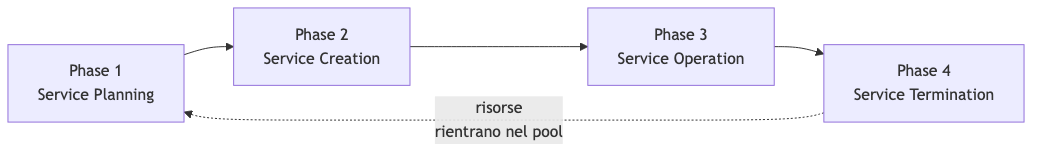
\includegraphics[keepaspectratio,alt={Diagramma Mermaid}]{images/mermaid-lezione-18-control-layer-orchestrazione-e-sla-01.png}}
\emph{Fig. --- Le quattro fasi del Cloud Service Lifecycle.}

\subsection{Phase 1: Service Planning}\label{phase-1-service-planning}

La fase di planning è \textbf{strategica}: si decide se vale la pena
creare un servizio. Il professore fa l'esempio dell'università: a un
certo punto si è valutata la domanda di web server per i professori
(siti di ricerca, didattica, etc.) e si è deciso di supportare solo
WordPress, semplificando il portfolio ma soddisfacendo la maggior parte
della domanda.

Le domande chiave del planning: - Quali servizi verranno creati o
aggiornati? Qual è il service model appropriato (IaaS, PaaS, SaaS)? -
Quali risorse hardware e software sono necessarie? - Chi sono i target
consumer? Qual è la domanda prevista? - Qual è il modello di deployment
(private, public, hybrid)? - Quali requisiti di compliance normativa
esistono?

\subsection{Billing Policy}\label{billing-policy}

Il billing non riguarda solo fare profitto. Il professore insiste su
questo punto: il cloud \textbf{nasconde i costi}. Quando si accede a un
servizio cloud dallo smartphone, non si pensa all'energia consumata dai
server, dagli switch, dai dischi. Se si archivia un documento inutile
nel cloud, si sta sprecando energia e denaro.

\begin{callouttip}{Esempio: Google Drive e i 100 TB}

Un collega del professore aveva accumulato 100 TB su Google Drive perché
un backup era partito con le impostazioni sbagliate e nessuno l'aveva
notato. Il problema era che quando il cloud era ``infinito'' e
``gratuito'', le persone non si rendevano conto dei costi. Google ha poi
reso lo storage limitato per lo stesso motivo: indurre le persone a
percepire il valore di ciò che consumano.

\end{callouttip}

Il billing è anche uno \textbf{strumento di policy}: si può aumentare il
prezzo di un servizio per scoraggiarne l'uso (es. un servizio energivoro
o meno verde) e abbassare quello di un alternativa preferita.
L'università di Pisa sta valutando di assegnare un ``budget IT
virtuale'' a ricercatori e staff, con la possibilità di scalare usando
fondi di ricerca se si supera la soglia --- proprio per creare
consapevolezza.

Tipi di billing nel private cloud: - \textbf{Chargeback}: il costo viene
effettivamente addebitato all'unità organizzativa. - \textbf{Showback}:
si mostra il costo senza addebitarlo, solo per trasparenza e
consapevolezza.

\subsection{Phase 2: Service Creation}\label{phase-2-service-creation}

Si definisce il \textbf{service template} (struttura del servizio,
attributi default, operazioni di gestione), si crea il \textbf{workflow
di orchestrazione} corrispondente e si definisce la \textbf{service
offering} nel catalogo. La service offering è la combinazione di:

\begin{itemize}
\tightlist
\item
  Template + struttura.
\item
  Constraints (chi può accedere).
\item
  Policy (QoS, firewall, bandwidth quota).
\item
  Rules (limiti di scaling, periodo di subscription).
\item
  Price.
\item
  \textbf{SLA} (Service Level Agreement).
\end{itemize}

\subsection{Phase 3: Service Operation}\label{phase-3-service-operation}

Gestione operativa continua: monitoring, reporting, provisioning di
nuove istanze, troubleshooting. L'obiettivo è automatizzare tutto il
possibile.

\subsection{Phase 4: Service
Termination}\label{phase-4-service-termination}

Quando un servizio viene terminato (per scelta del provider, del
consumer, o per fine contratto), tutte le risorse vengono rilasciate e
restituite al pool. La terminazione non deve impattare altri servizi né
i dati dei consumer.

\begin{center}\rule{0.5\linewidth}{0.5pt}\end{center}

\section{Service Level Agreement
(SLA)}\label{service-level-agreement-sla-1}

Il professore dedica la parte finale della lezione all'SLA,
considerandolo uno dei documenti più importanti --- e più trascurati dai
tecnici --- nel cloud.

\begin{calloutdefinition}{Service Level Agreement (SLA)}

Contratto che definisce la \textbf{qualità di servizio} che il provider
garantisce al consumer. Non si acquista hardware specifico: si acquista
un livello di qualità indipendentemente da come il provider lo realizzi.

\end{calloutdefinition}

Il cloud è ``somewhere'': non si sa su quale disco, in quale datacenter,
in quale paese siano i propri dati. L'SLA è l'unico strumento
contrattuale che garantisce che il servizio ricevuto corrisponda a
quello pagato.

\subsection{Domande chiave dell'SLA}\label{domande-chiave-dellsla}

\begin{calloutquestion}{Domande chiave dell’SLA}

\begin{enumerate}
\def\labelenumi{\arabic{enumi}.}
\tightlist
\item
  Quali sono i livelli minimi accettabili di performance e
  disponibilità?
\item
  C'è un limite alla quantità di risorse consumabili?
\item
  Come viene definita un'interruzione di servizio? Come vengono
  compensati i consumer?
\item
  Qual è il livello di servizio durante i periodi di manutenzione?
\item
  I consumer devono pagare licenze aggiuntive oltre ai costi del
  servizio?
\item
  Dove verrà archiviata la copia primaria dei dati? Come sarà protetta?
\item
  Vengono offerti compliance e data security come servizi supplementari?
\item
  I consumer verranno notificati se un'agenzia governativa richiede i
  loro dati?
\item
  Quali garanzie di customer service e tempi di risposta sono previste?
\end{enumerate}

\end{calloutquestion}

\textbf{Sul punto 1}: il costo aumenta in modo non lineare con il
livello di disponibilità. Garantire il 95\% di uptime costa
relativamente poco; garantire il 99.99\% richiede ridondanze massicce
che si riflettono sul prezzo.

\textbf{Sul punto 3}: la definizione di ``service outage'' è il punto
più critico e insidioso dell'SLA. È qui che i provider hanno margine di
manovra legale.

\textbf{Sul punto 6}: per le pubbliche amministrazioni europee, i dati
devono risiedere in datacenter europei (GDPR). L'SLA deve specificare
esplicitamente la geolocalizzazione dei dati.

\textbf{Sul punto 8}: dopo gli attentati dell'11 settembre 2001, il
governo USA si è riservato il diritto di accedere a email e
comunicazioni di sospetti terroristici senza notificare gli interessati.
Un SLA con un provider americano potrebbe non garantire notifica in caso
di richieste di accesso governativo.

\subsection{La Definizione di Downtime: il Punto
Critico}\label{la-definizione-di-downtime-il-punto-critico}

Il professore sottolinea che la prima cosa da leggere in un SLA non è la
tabella delle compensazioni, ma la \textbf{sezione delle definizioni}
--- in particolare la definizione di downtime.

\begin{calloutwarning}{Trucchi nella definizione di downtime}

\begin{itemize}
\tightlist
\item
  \textbf{Misura in user-minutes}: il downtime non si misura in minuti
  di clock, ma in (minuti × utenti impattati). Se il problema riguarda
  solo un account su 50.000, l'impatto in user-minutes è quasi zero ---
  quindi non viene contato come downtime.
\item
  \textbf{Slot minimi}: Amazon nel suo primo SLA dichiarava che
  un'interruzione veniva contata solo se la VM non era accessibile per
  almeno 5 minuti. Interruzioni da 4 minuti non esistevano. Molte
  interruzioni brevi potevano accumularsi senza essere conteggiate.
\item
  \textbf{Colpa di terze parti}: se il problema è nella rete del
  provider internet del consumer, o nel laptop del consumer, non è colpa
  del cloud provider.
\item
  \textbf{Scheduled downtime}: la manutenzione pianificata e notificata
  con almeno 5 giorni di anticipo non conta come downtime.
\end{itemize}

\end{calloutwarning}

\subsection{Caso Pratico: Microsoft 365
SLA}\label{caso-pratico-microsoft-365-sla}

Il professore apre live il documento SLA di Microsoft 365 e analizza le
sezioni chiave.

\textbf{Definizione di Uptime Percentage}:

\[
\text{Uptime \%} = \frac{\text{User Minutes} - \text{Downtime}}{\text{User Minutes}} \times 100
\]

Dove: - \textbf{User Minutes} = (minuti totali nel periodo − scheduled
downtime) × numero di utenti. - \textbf{Downtime} = Σ (durata incidente
in minuti × utenti impattati dall'incidente).

\textbf{Scheduled Downtime}: ``We will publish notice at least five days
prior to the downtime.'' Se la notifica arriva tardi, quella
manutenzione non è più ``scheduled downtime'' --- è vera interruzione.

\textbf{Service Credits} (compensazioni):

{\def\LTcaptype{none} % do not increment counter
\begin{longtable}[]{@{}ll@{}}
\toprule\noalign{}
Uptime \% & Credito \\
\midrule\noalign{}
\endhead
\bottomrule\noalign{}
\endlastfoot
\textless{} 99.9\% & 25\% \\
\textless{} 99\% & 10\% \\
\textless{} 95\% & 50\% \\
Sotto ogni soglia garantita & 100\% \\
\end{longtable}
}

\begin{calloutnote}{I crediti sono crediti, non rimborsi}

Microsoft (e la quasi totalità dei provider) restituisce il valore sotto
forma di \textbf{crediti di servizio}, non di denaro. Il consumer deve
fare un claim, Microsoft deve approvarlo, e solo allora riceve crediti
da spendere su servizi Microsoft.

\end{calloutnote}

\begin{callouttip}{Impatto pratico della misura in user-minutes}

Se un'interruzione dura 1 ora e impatta solo il tuo account su 50.000
utenti dell'Università di Pisa, il downtime in user-minutes è 60 × 1 =
60 user-minutes. I total user-minutes del mese sono ≈ 50.000 × 43.200 =
2.160.000.000. L'impatto percentuale è trascurabile --- praticamente
zero ai fini del calcolo dell'SLA.

\end{callouttip}

\subsection{Il Messaggio Finale}\label{il-messaggio-finale}

Il professore chiude con una riflessione: i tecnici tendono a guardare
solo se il servizio è su o giù, senza preoccuparsi delle implicazioni
legali. Ma stiamo entrando in un mondo in cui i sistemi digitali sono il
corrispettivo del mondo reale: se i sistemi informatici universitari
sono down il giorno della laurea per colpa del CIO, i danni sono reali e
le responsabilità legali pure.

\begin{calloutnote}{Sintesi}

Il cloud non è solo tecnologia: è un sistema sociotecnico con
implicazioni legali, economiche e organizzative. Il Control Layer
gestisce l'infrastruttura in modo automatizzato e scalabile. Il Service
e Orchestration Layer espongono questa infrastruttura come servizi
consumabili. L'SLA è il contratto che definisce le garanzie --- e la sua
comprensione richiede attenzione legale, non solo tecnica.

\end{calloutnote}

\newpage

\backmatter
\end{document}
